%
% Het bestand thesis.tex wordt iedere keer als make aangeroepen wordt
% opnieuw opgebouwd. Wijzigingen in thesis.tex zelf zullen verloren gaan!
% 
\documentclass{main/thesis}
\usepackage{amssymb}
\usepackage[dutch]{babel}
\usepackage{datetime}
\usepackage{graphicx}
\usepackage{color}
\usepackage{epstopdf}
\DeclareGraphicsRule{.eps}{pdf}{.pdf}{`epstopdf #1}
\usepackage{chapterbib}
\usepackage{ifthen}
\usepackage[pdftex,bookmarks=true,hidelinks,pdfauthor={Jeroen Engelberts},pdftitle={Valence Bond Theory: A Toolkit For The Analysis Of Chemical Bonding},pdfsubject={Valence Bond Theory}]{hyperref}
\usepackage{lettrine}
\usepackage{yfonts}
\usepackage[T1]{fontenc}
\newcommand{\vbbox}[2]
{
   \begin{minipage}{\textwidth}
      \vspace{12pt}
      \center
      \colorbox{grey1}{\parbox{\textwidth}{\textbf{Example #2}
   \texttt{#1}}}
   \end{minipage}
   \vspace{1pt}
}

% Float placement ...
\renewcommand{\topfraction}{0.8}
\renewcommand{\bottomfraction}{0.8}
\renewcommand{\textfraction}{0.1}
\renewcommand{\floatpagefraction}{0.8}

\setcounter{topnumber}{2}       % Maximum # of floats at top of page
\setcounter{bottomnumber}{2}    % Maximum # of floats at bottom of page
\setcounter{totalnumber}{3}     % Maximum total # of floats on one page
\newboolean{wholethesis}
\setboolean{wholethesis}{false}     % Used for date on separate chapters

%Double line spacing if necessary
\renewcommand{\baselinestretch}{1.2}

\vfuzz1pc   % Don't bother to report overfull boxes if over-edge is < 1pc
\hfuzz1pc   % Don't bother to report overfull boxes if over-edge is < 1pc

%Manual commands

%Highlight color \mx{this has been changed}
\definecolor{orange}{rgb}{1,0.5,0}
\definecolor{purple}{rgb}{1,0,1}
\newcommand{\mg}[1]{\color{green}{#1}\normalcolor}
\newcommand{\mo}[1]{\color{orange}{#1}\normalcolor}
\newcommand{\my}[1]{\color{yellow}{#1}\normalcolor}
\newcommand{\mr}[1]{\color{purple}{#1}\normalcolor}
\newcommand{\mc}[1]{\color{cyan}{#1}\normalcolor}
%Symbol for degrees (angles and temperature)
\newcommand{\degrees}{$^{\mathrm{o}}$}
%Easy reference to chapters
\newcommand{\chintro}{\ifthenelse{\boolean{wholethesis}}{\ref{chap_intro}}{1}}
\newcommand{\chorbopt}{\ifthenelse{\boolean{wholethesis}}{\ref{chap_orbopt}}{2}}
\newcommand{\chdissociation}{\ifthenelse{\boolean{wholethesis}}{\ref{chap_dissociation}}{3}}
\newcommand{\chcyclopentadienyl}{\ifthenelse{\boolean{wholethesis}}{\ref{chap_cyclopentadienyl}}{4}}
\newcommand{\chhuckel}{\ifthenelse{\boolean{wholethesis}}{\ref{chap_huckel}}{5}}
\newcommand{\chinorganic}{\ifthenelse{\boolean{wholethesis}}{\ref{chap_inorganic}}{6}}
\newcommand{\chindacene}{\ifthenelse{\boolean{wholethesis}}{\ref{chap_indacene}}{7}}
%Nice letter in each chapter (see http://www.tug.dk/FontCatalogue/otherfonts.html#initials)
\input RoyalIn.fd
\newcommand*\initial{\usefont{U}{RoyalIn}{xl}{n}\selectfont}

\begin{document}
\setboolean{wholethesis}{true}
%\title{Valence Bond Theory: A Toolkit For The Analysis Of Chemical Bonding}

%\frontmatter
\pagestyle{empty}

\typeout{******** Titlepage and preamble ********}

%\maketitle
\clearpage

\mbox{}

\begin{otherlanguage*}{dutch}

\begin{center}
\Huge{Valence Bond Theory: A Toolkit For The Analysis Of Chemical Bonding}

\vskip 1em%

\LARGE{Valence Bond Theorie: Hulpmiddel Voor De Analyse Van Chemische Binding}

\vskip 1em%

\normalsize (met een samenvatting in het Nederlands)
\end{center}

\vspace{\fill}

\begin{center}
\LARGE{Proefschrift}
\end{center}

\vskip 1em%

\noindent Ter verkrijging van de graad van doctor aan de Universiteit Utrecht op gezag van de Rector Magnificus, Prof. Dr. W.~H. Gispen, in gevolge het besluit van het College voor Promoties in het openbaar te verdedigen op weekdag dag~maand~jaar des dagdeels te hh:mm~uur

\vskip 1em%

\begin{center}
door

\vskip 1em%

\LARGE{Jeroen Johan Engelberts}

\vskip 1em%

\normalsize geboren op 7 december 1972 te Rotterdam
\end{center}
\newpage

\begin{tabbing}
Co-promotoren: \= \kill\\
Promotor: \>Prof. Dr. L. W. Jenneskens\\
          \>Verbonden aan het Departement Scheikunde,\\
          \>Universiteit Utrecht\\
\\
Co-promotor: \>Dr. R. W. A. Havenith\\
             \>Verbonden aan ...,\\
             \>Universiteit Groningen\\  
\\
\end{tabbing}

%\vspace{\fill}

\newpage
\mbox{ }\\
\mbox{ }\\
\mbox{ }\\
\mbox{ }\\
\mbox{ }\\
\mbox{ }\\
\mbox{ }\\
\mbox{ }\\
\mbox{ }\\
\mbox{ }\\
\mbox{ }\\
\mbox{ }\\
\mbox{ }\\
\mbox{ }\\
\mbox{ }\\
\mbox{ }\\
\mbox{ }\\
\mbox{ }\\
\mbox{ }\\
\mbox{ }\\
\mbox{ }\\
\mbox{ }\\
\mbox{ }\\
\mbox{ }\\
\mbox{ }\\
\mbox{ }\\
\mbox{ }\\
\mbox{ }\\
\mbox{ }\\
\mbox{ }\\
\mbox{ }\\
\mbox{ }
\raggedleft
\textit{Voor Eveline}

\newpage
\raggedright
\noindent
\begin{tabbing}
Never give \= up and \kill\\
\textit{"Never give up and good luck will find you."}\\
\> - Falcor, The Neverending Story, 1984.
\end{tabbing}
\mbox{ }\\
\mbox{ }\\
\mbox{ }\\
\mbox{ }\\
\mbox{ }\\
\mbox{ }\\
\mbox{ }\\
\mbox{ }\\
\mbox{ }\\
\mbox{ }\\
\mbox{ }\\
\mbox{ }\\
\mbox{ }\\
\mbox{ }\\
\mbox{ }\\
\mbox{ }\\
\mbox{ }\\
\mbox{ }\\
\mbox{ }\\
\mbox{ }\\
\mbox{ }\\
\mbox{ }\\
\mbox{ }\\
\mbox{ }\\
\mbox{ }\\
\begin{tabbing}
Paranimfen: \=Heleen van den Boom\\
            \>Sonja Coors
\end{tabbing}
Cover design by Roel Savert\\
\mbox{ }\\
Printed by PrintPartners IPSKAMP\\
\mbox{ }\\
Valence Bond Theory: A Toolkit For The Analysis Of Chemical Bonding\\
Jeroen Johan Engelberts\\
Ph. D. Thesis Utrecht University, \today \\
ISBN:~XX-YYYYYY-Z
\newpage

\end{otherlanguage*}

\tableofcontents

\mainmatter \pagestyle{fancy}


\setcounter{chapter}{0}
\setcounter{NAT@ctr}{0}
\chapter{Introduction}
\label{chap_intro}

\hyphenation{para-mag-net-ic}

\ifthenelse{\boolean{wholethesis}}{\relax}{\begin{center}\textit{Generated on \today\ at \currenttime}\end{center}}
\newpage

\section{\label{ch1.sec.history1}From Alchemy to Chemistry}

\lettrine{\initial{F}}{}or nearly 2000 years, scholars believed that everything was made up of combinations of just four elements: air, earth, fire and water. This belief survived until the 17$^\mathrm{th}$ century. One of the first to doubt the original principles was Boyle. In his book \textit{The Skeptical Chymist}, published in 1661, he wrote that matter is composed of elemental particles and that changes in matter are caused by rearrangement of these elemental particles \cite{boyle}. One of the aspects of early chemistry, or alchemy, that Boyle did not challenge was the so-called \textit{phlogiston} theory. Until the 18$^\mathrm{th}$ century, it was generally believed that fire (or \textit{phlogiston}) was part of matter. Metals, for example, were thought to be a combination of earth and fire, because when a metal was burnt the \textit{phlogiston} left the metal and only the residual earth (metal oxide) was left. In 1789 de Lavoisier, writer of the famous book \textit{Trait\'e \'El\'ementaire de Chimie} \cite{lavoisier}, countered this belief by pointing out that this earth, left after burning of the metal, weighed more than the metal itself. With later experiments the existence of oxygen was proven and the increase of weight could now be understood.

Several elements, like carbon and iron have been known from antiquity. In the late 18$^\mathrm{th}$ and early 19$^\mathrm{th}$ centuries more and more elements were discovered, like chromium (Cr), beryllium (Be) and titanium (Ti).  In 1869 Mendeleev ordered the known elements on their mass \cite{mendeleev}. Mendeleev had the audacity to leave open spaces in his table for elements that were not yet discovered. He went even further by predicting some properties of those elements by looking at the properties of elements in the same column. In the subsequent years his predictions were confirmed when the three elements, gallium (Ga), germanium (Ge) and scandium (Sc) were identified, filling their open spaces in the periodic table.

At the dawn of the 20$^\mathrm{th}$ century people, like Thomson and Lewis, were studying the way atoms bind together. Until then atoms were thought to be indivisible, as the Greek word \textit{atomos} implies. Thomson, however, pointed out that the linkages between atoms are caused by the transfer of ``corpuscles'', stating: ``For each valency bond established between two atoms the transference of one corpuscle from the one atom to the other has taken place, the atom receiving the corpuscle acquiring a unit charge of negative electricity, the other by the loss of a corpuscle acquiring a unit charge of positive \cite{thomson}.'' These valency (electrostatic) bonds were schematically represented with arrows (Figure \ref{ch1.fig1}). The carbon atom in methane (CH$_4$) has taken up four electrons, while in tetrachloromethane (CCl$_4$), it has lost four. The arrows indicate the transfer direction of the electrons. 
\begin{figure}[htp]
\center
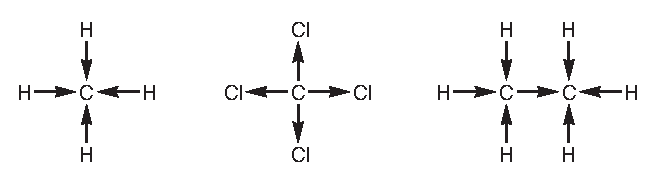
\includegraphics[width=4in]{introduction/figures/figure1.eps}
\caption{Schematic representation of the bonds in methane, tetrachloromethane and ethane \cite{falk}.}
\label{ch1.fig1}
\end{figure}
The situation with the ``equivalent'' carbon atoms in ethane was described by Falk and Nelson: ``In ethane (C$_2$H$_6$), therefore, one of the carbon atoms will have a charge of four units of negative electricity and the other of two units, or comparing the carbon atoms of the two methyl groups, one will be negatively charged and the other positively charged \cite{falk}.'' Thomson, however, already doubted this mechanism and indicated that it was not yet fully understood \cite{thomson}.

In 1916 Lewis introduced a set of postulates still used in chemistry today \cite{lewis}. He refined the classical electrostatic view of Falk and Nelson by writing that the electrostatic forces between particles which are close together do not obey the simple law of inverse squares which holds at greater distances. Lewis also suggested that atoms tend to assume the electronic configuration of a noble gas, through electron transfer or through the sharing of electrons with other atoms, and that the eight outermost electrons in an atom with a noble-gas electronic structure are arranged tetrahedrally in pairs about the atom. Furthermore, Lewis introduced in this article a new way of representing chemical bonds, which is shown in Figure \ref{ch1.fig2}. These representations show that the carbon atoms in methane, as well as in ethane, acquired a noble-gas configuration, which is known nowadays as the \textit{octet rule} \cite{bruice}.
\begin{figure}[htp]
\center
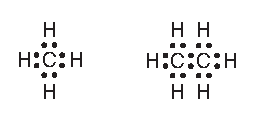
\includegraphics[width=2in]{introduction/figures/figure2.eps}
\caption{The Lewis representation of the bonds in methane and ethane \cite{lewis}.}
\label{ch1.fig2}
\end{figure}

\section{Quantum Mechanics in Chemistry}

In the 1920s the physicists Heisenberg and Schr\"{o}dinger, amongst others, developed the quantum mechanics. Heisenberg formulated his theory in terms of matrices \cite{heisenberg}, while Schr\"{o}dinger used wave functions \cite{schrodinger1,schrodinger2}. Both formulations are equivalent \cite{schrodinger3}. For the work described in this thesis, only the so-called time independent, non-relativistic Schr\"{o}dinger equation is used:
\begin{equation}
\mathbf{H} \Psi=E \Psi.
\label{ch1.eq.hpsi}
\end{equation}
For each (chemical) system a Hamilton operator ($\mathbf{H}$) can be defined. This Hamiltonian contains terms to obtain the kinetic energy of the nuclei and electrons ($\mathbf{T}_n$ and $\mathbf{T}_e$) and the potential energy of the nuclei and electrons, \textit{i.e.} Coulomb repulsion between nuclei ($\mathbf{V}_{nn}$), Coulomb repulsion between electrons ($\mathbf{V}_{ee}$), and Coulomb attraction between nuclei and electrons ($\mathbf{V}_{en}$):
\begin{equation}
\mathbf{H} = \mathbf{T}_n + \mathbf{T}_e + \mathbf{V}_{nn} + \mathbf{V}_{ee} + \mathbf{V}_{en}.
\label{ch1.eq.htotal}
\end{equation}
By solving equation \ref{ch1.eq.hpsi} all information about the system is accessible. Solving this equation, however, poses a real challenge, since it can only be solved analytically for the simplest cases. For all other systems, like the molecules described in this thesis, approximations are applied.

The first approximation considered is the Born-Oppenheimer approximation \cite{born}. In this approximation, the Hamiltonian is written as a sum of terms for the nuclei and the electrons:
\begin{equation}
\mathbf{H} = \mathbf{H}_n + \mathbf{H}_e = (\mathbf{T}_n + \mathbf{V}_{nn}) + (\mathbf{T}_e + \mathbf{V}_{ee} + \mathbf{V}_{en}).
\label{ch1.eq.hsplit}
\end{equation}
$\Psi$ can then be approximated by a product of a wave function for the nuclei and one for the electrons. Because of the term $\mathbf{V}_{en}$, $\Psi_{e}$ depends parametrically on the coordinates of the nuclei:
\begin{equation}
\Psi \approx \Psi_{n}(\mathrm{X}) \Psi_{e}(\mathrm{q,X}).
\end{equation}
One assumption in the Born-Oppenheimer approximation is that the electronic wave function $\Psi_{e}$ does not change much for small variations in the positions of the nuclei ($\mathrm{X}$) \cite{born}. On the other hand, it is assumed that the motion of the nuclei, which are much heavier than the electrons, does depend on the electron density, rather than on the positions of the individual electrons. With those approximations, the total energy ($E_\mathrm{tot}$) can be written as the sum of a contribution of the nuclei and one of the electrons:
\begin{equation}
E_\mathrm{tot} = \frac{\mathbf{H}_n \Psi_n(\mathrm{X})}{\Psi_n(\mathrm{X})} + \frac{\mathbf{H}_e \Psi_e(\mathrm{q,X})}{\Psi_e(\mathrm{q,X})} = E_{n} + E_{e}.
\end{equation}

Several types of approximations for the wave functions ($\Psi$) have been defined to describe chemical systems. All these wave functions have in common that they are expressed in molecular orbitals ($\psi$), which are linear combinations of atomic orbitals (AOs) $\phi$, or basis functions (LCAO MOs):
\begin{equation}
\psi = c_1 \phi_1 + c_2 \phi_2 + \cdots + c_n \phi_n = \sum_n c_n \phi_n.
\label{ch1.eq.lcaomo}
\end{equation}
The molecular orbitals (MOs) are functions of the coordinates of the electrons (spatial orbitals), or of the coordinates \textit{and} the spins of the electrons (spin orbitals). The spin of an electron can be one of two states. Commonly, these states are referred to as $\alpha$ and $\beta$ spin. The term ``doubly occupied molecular orbital'' indicates that there are two electrons with the same spatial orbital, but with opposite spins.

\subsection{Hartree Products and Slater Determinants}

Multi-electron wave functions are either written as Hartree products \cite{hartree1,hartree2,hartree3} or as Slater determinants \cite{slater}. In a Hartree product the wave function is written as a product:
\begin{equation}
\Psi=\prod_i \psi_i(\mathbf{\tau}_i),
\end{equation}
in which the parameters $\mathbf{\tau}_i$ contain the spatial and spin coordinates of the electrons. This type of wave function is used in the H\"uckel method \cite{huckel1,huckel2,huckel3}. Characteristic for Hartree product wave functions is that they do not fulfill the antisymmetry principle \cite{atkins}. This principle states that the total wave function must change sign when the spatial and spin coordinates of two electrons are interchanged, which is the case when the wave function is written as a determinant. In such a determinant, referred to as Slater determinant in quantum chemistry, the sign of the wave function changes:
\begin{equation}
\begin{split}
\Psi_1 &=
\begin{array}{|cc|}
\psi_1(\mathbf{\tau_1}) & \psi_2(\mathbf{\tau_1}) \\
\psi_1(\mathbf{\tau_2}) & \psi_2(\mathbf{\tau_2}) \\
\end{array}
= \psi_1(\mathbf{\tau_1})\psi_2(\mathbf{\tau_2}) - \psi_1(\mathbf{\tau_2})\psi_2(\mathbf{\tau_1}), \\
\Psi_2 &=
\begin{array}{|cc|}
\psi_1(\mathbf{\tau_2}) & \psi_2(\mathbf{\tau_2}) \\
\psi_1(\mathbf{\tau_1}) & \psi_2(\mathbf{\tau_1}) \\
\end{array}
= \psi_1(\mathbf{\tau_2})\psi_2(\mathbf{\tau_1}) - \psi_1(\mathbf{\tau_1})\psi_2(\mathbf{\tau_2}), \\
\Psi_1 &= - \Psi_2
\end{split}
\label{ch1.eq.slater}
\end{equation}
A nice aspect of writing the wave function as a determinant is that it automatically becomes zero in the case of the occurence of two orbitals with the same spatial \textit{and} spin coordinates. This effect is linked to the Pauli exclusion principle, which practically translates into the rule that no two electrons can occupy the same spin orbital. In that case, the determinant contains two identical columns and hence becomes zero.

Throughout the years, many quantum chemical methods have been developed based on Slater determinants and molecular orbitals (MOs). These methods are described in quantum chemical textbooks \cite{szabo}. Here, the methods used throughout this thesis will be introduced briefly.

\subsection{The Hartree-Fock (HF) Method}
The simplest way to find approximate solutions for the Schr\"{o}dinger equation (equation \ref{ch1.eq.hpsi}) is with the help of a function where the N-electron wave function is approximated by a single Slater determinant (equation \ref{ch1.eq.slater}), $\Psi_\mathrm{HF}$. This is called the Hartree-Fock method \cite{hartree1,hartree2,hartree3,fock}. For a normalized wave function ($\left< \Psi_\mathrm{HF} | \Psi_\mathrm{HF} \right> = 1$), the energy ($E$) is calculated as an expectation value of the Hamiltonian ($\mathbf{H}$):
\begin{equation}
E=\left< \Psi_\mathrm{HF} | \mathbf{H} | \Psi_\mathrm{HF} \right>,
\label{ch1.eq.hfexp}
\end{equation}
where $\Psi_\mathrm{HF}$ is the single determinant Hartree-Fock wave function constructed from orthonormal orbitals $\psi_i$.

With the Hamiltonian of equation \ref{ch1.eq.htotal}, the expression for the energy ($E$) becomes:
\begin{equation}
E=\sum_i h_{ii} + \frac{1}{2} \sum_i\sum_j (J_{ij} - K_{ij}) + \mathbf{V}_{nn},
\label{ch1.eq.hfexp_detailed}
\end{equation}
where $h_{ii}$:
\begin{equation}
h_{ii} = \left< \psi_i(\tau_1) | \mathbf{T}_{e}(\tau_1) + \mathbf{V}_{en}(\tau_1) | \psi_i(\tau_1)\right>,
\end{equation}
describes the kinetic energy of electron $\tau_1$ and its attraction to the nuclei.

The second term on the right hand side of equation \ref{ch1.eq.hfexp_detailed} contains the so-called Coulomb ($J_{ij}$) and exchange ($K_{ij}$) interactions. These arise from the electron-electron repulsion term $\mathbf{V}_{ee}$ in the Hamilton operator (equation \ref{ch1.eq.htotal}). The exchange interaction is present because Slater determinants are used. This is exemplified with the help of the Slater determinant ($\Psi_1$) of equation \ref{ch1.eq.slater}:
\begin{equation}
\begin{split}
\left< \Psi_1 | \mathbf{V}_{ee} | \Psi_1 \right> = & \left< \psi_1(\mathbf{\tau_1})\psi_2(\mathbf{\tau_2}) | \frac{1}{r_{12}} | \psi_1(\mathbf{\tau_1})\psi_2(\mathbf{\tau_2}) \right> - \\
& \left< \psi_1(\mathbf{\tau_1})\psi_2(\mathbf{\tau_2}) | \frac{1}{r_{12}} | \psi_2(\mathbf{\tau_1})\psi_1(\mathbf{\tau_2}) \right> \\
= & J_{12} - K_{12}, \\
\end{split}
\end{equation}
where $\frac{1}{r_{12}}$ is the electron-electron repulsion operator.

Because the Born-Oppenheimer approximation (the motions of nuclei and electrons are split) is applied, the kinetic operator ($\mathbf{T}_{n}$) is absent in equation \ref{ch1.eq.hfexp_detailed}. The nuclei-nuclei repulsion ($\mathbf{V}_{nn}$) adds a constant contribution to the energy ($E$) in equation \ref{ch1.eq.hfexp_detailed} for fixed molecular geometries.

The orbitals in wave function $\Psi_\mathrm{HF}$ are optimized with the goal of finding the minimum, or at least a stationary point, for the expectation value $E$ in equation \ref{ch1.eq.hfexp}, using the variation principle \cite{varia}. During the optimization the orbitals are modified, but are kept orthonormal. The minimization of the energy with respect to change in the orbitals leads to the following Hartree-Fock equations:
\begin{equation}
\mathbf{F}(i)\psi_j(i)=\epsilon_j \psi_j(i),
\label{ch1.eq.fock1}
\end{equation}
in which $\mathbf{F}(i)$ is the so called one electron Fock operator, which is written as:
\begin{equation}
\mathbf{F}(i)=\mathbf{h}(i) + \sum_j (\mathbf{J_j}(i) - \mathbf{K_j}(i)).
\label{ch1.eq.fock2}
\end{equation}
Since the Fock operator depends on the orbitals it operates on, the Hartree-Fock equations (\ref{ch1.eq.fock1} and \ref{ch1.eq.fock2}) are solved in an iterative manner, referred to as the Self Consistent Field (SCF) method.

The optimization is performed by modifying the coefficients $c_n$ for the atomic orbitals in equation \ref{ch1.eq.lcaomo}. With the Fock operator, applied to the atomic orbitals (AOs), the orbital energies ($\epsilon_j$) are obtained:
\begin{equation}
\mathbf{F}\sum_n c_n \phi_n (i) = \epsilon_j \sum_n c_n \phi_n (i).
\label{ch1.eq.fockao}
\end{equation}

Equation \ref{ch1.eq.fockao} can be written in matrix form by multiplying from the left with an atomic orbital and integrating:
\begin{equation}
\mathbf{F}\mathbf{C} = \mathbf{S}\mathbf{C}\mathbf{\epsilon},
\label{ch1.eq.fockmatrixs}
\end{equation}
in which $\mathbf{F}$ is the Fock matrix, $\mathbf{S}$ the orbital overlap matrix and $\mathbf{\epsilon}$ the matrix of orbital energies. The $\mathbf{S}$ matrix is present, because the basis functions $\phi_n$ are not orthogonal. However, linear combinations can be chosen in such a way that the basis becomes orthogonal. With such a transformation $\mathbf{S}$ becomes a unity matrix and equation \ref{ch1.eq.fockmatrixs} becomes:
\begin{equation}
\mathbf{F'}\mathbf{C'} = \mathbf{C'}\mathbf{\epsilon}.
\end{equation}

In the Hartree-Fock method the most commonly used type of wave function is a single determinant with doubly occupied orbitals, \textit{i.e.} two electrons per orbital with paired spins. This is referred to as closed-shell and the wave function is called restricted Hartree-Fock (RHF). If not all orbitals are doubly occupied, \textit{i.e.} not all electrons are paired, the wave function is referred to as restricted open-shell Hartree-Fock (ROHF). When different spatial orbitals are used for electrons with $\alpha$ and $\beta$ spin, the method is referred to as unrestricted Hartree-Fock (UHF). An advantage of UHF over ROHF is that it gives a correct description of the dissociation of molecules into atoms or molecular fragments, for example. A disadvantage of UHF, however, is that the wave function is not a proper eigenfunction of the total spin operator $\mathbf{S}^2$.

A property of the single determinant in the Hartree-Fock method is that each electron moves in the average electric field created by the other electrons, \textit{i.e.} there is no electron correlation. For a more accurate expression, the instantaneous interaction between the electrons must be taken into account. Electronic structure methods that take care of electron-electron interaction are called electron correlation methods. The difference between the Hartree-Fock energy ($E_\mathrm{HF}$) and the exact energy is called the \textit{correlation energy}. Three of these methods, the Configuration Interaction Method (CI) \cite{shavitt1,shavitt2}, Multi Configuration Self Consistent Field Method (MCSCF) \cite{daswahl,wahldasbook,mcscf,roos1,roos2} and the Coupled Cluster Method (CC) \cite{cc1,cc2}, will be introduced here.

\subsection{\label{ch1.sec.ci}The Configuration Interaction (CI) Method}

A Configuration Interaction (CI) wave function is created from a reference function ($\Phi_0$), quite often a Hartree-Fock wave function ($\Phi_0 = \Psi_\mathrm{HF}$), with the help of an excitation operator $\mathbf{T}$:
\begin{equation}
\mathbf{T}=\mathbf{T}_1 + \mathbf{T}_2 + \mathbf{T}_3 + ... + \mathbf{T}_{N_{\mathrm{elec}}},
\label{ch1.eq.ciexcitation}
\end{equation}
in which $\mathbf{T}_1$ is a single excitation operator, $\mathbf{T}_2$ a double excitation operator and $\mathbf{T}_{N_{\mathrm{elec}}}$ the operator that excites \textit{all} $N_{\mathrm{elec}}$ electrons in the molecule. The excitation results in excited Configuration State Functions (CSFs) \cite{shavitt1,shavitt2}. A CSF ($\Phi_k$) is constructed from one or more Slater determinants in such a way that it is an eigenfunction of the N-electrons' spin operators $\mathbf{S}^2$ and $\mathbf{S}_z$. Single and double excited CSF are created by $\mathbf{T}_1$ and $\mathbf{T}_2$, respectively:
\begin{equation}
\begin{split}
\mathbf{T}_1 \Phi_0 & = \sum_i^{occ} \sum_a^{vir} c_i^a \Phi_i^a \\
\mathbf{T}_2 \Phi_0 & = \sum_{i<j}^{occ} \sum_{a<b}^{vir} c_{ij}^{ab} \Phi_{ij}^{ab},
\end{split}
\label{ch1.eq.ciexcited}
\end{equation}
in which $\Phi_i^a$ and $\Phi_{ij}^{ab}$ are singly and doubly excited CSFs, respectively. The coefficients $c_i^a$ and $c_{ij}^{ab}$ are determined with the help of the variation principle. The total CI wave function ($\Psi_{\mathrm{CI}}$) is constructed from a linear combination of these excited CSFs:
\begin{equation}
\Psi_{\mathrm{CI}} = \sum_{k}^{N_{\mathrm{CSF}}} c_k \Phi_k,
\label{ch1.eq.ci}
\end{equation}
in which $k$ runs over all CSFs. The coefficients $c_k$ are determined by the variational principle \cite{varia}, while the orbitals inside $\Phi_k$ are kept fixed. A wave function containing all possible CSFs in equation \ref{ch1.eq.ci} for a given basis set is called a full CI wave function. Solving the Schr\"{o}dinger equation \ref{ch1.eq.hpsi} with full CI gives the ``exact'' energy for that given basis set. In full CI, the number of CSFs is accompanied by a factorial increase with the number of electrons and the size of the basis set \cite{weyl}. Therefore, a full CI wave function is only feasible for very small molecular systems. In practice, the CI expansion is truncated and only a subset of the possible CSFs is included in the wave function. These truncations are labeled with capitals S, D, T, Q to indicate that only singly, doubly, triple, or quadruple excited configurations are included in the expansion. For example, in a CISD wave function only singly and doubly excited CSFs are included in the expansion.

A disadvantage of such a truncation is that the wave function is no longer size consistent, \textit{i.e.} the wave function for two molecules at large distance from each other has a higher energy than the sum of the individual energies. For example, a CISD expanded wave function for a single H$_2$ molecule contains the CSF describing the doubly excited state. Although, for a combination of two H$_2$ molecules at large distance, double excitations do occur within each molecule, the CSF in which \textit{both} H$_2$ molecules are doubly excited at the \textit{same} time does not occur, since this would be a quadruple excitation.

Although CI wave functions have not been used for the calculations described in this thesis, in the Valence Bond Configuration Interaction method, described later in this chapter, the same principle of optimizing the CSF, or structure, coefficients with fixed orbitals is applied.

\subsection{\label{ch1.sec.mcscf}The Multi Configuration Self Consistent Field (MCSCF) Method}
Like in CI, Multi Configuration Self Consistent Field (MCSCF) wave function are expressed in Configuration State Functions (CSFs) \cite{wahldasbook,daswahl}. In contrast with CI, both the orbital \textit{and} the expansion coefficients are optimized in MCSCF.

In an MCSCF wave functions the orbitals are divided over two sets. One set contains the orbitals that are doubly occupied in all CSFs (inactive) and the other set contains the variably occupied orbitals (active). In the active space the CSFs are generated by distributing active electrons over the active orbitals in all possible ways. This can be considered as a full CI in the active space. In literature, two designations for this type of method are found. It is referred to as the Fully Optimized Reaction Space (FORS) method \cite{fors1,fors2,fors3} and as Complete Active Space SCF (CASSCF) \cite{roos1,roos2}.

Although MCSCF is not used for calculations described in this thesis, it has much in common with the Valence Bond Self Consistent field method, described later in this chapter. For example, the latter is expressed in structures, comparable to CSFs, for which both the orbitals coefficients and the expansion coefficients are optimized. 

One mechanism that can be used for this optimization is the so called Super CI \cite{superci1,superci2} method (\textit{cf.} Chapter \chorbopt). Within this method the wave function is expanded with singly excited CSFs. For this expanded wave function the CI (or Brillouin) vector $\mathbf{b}$ is determined by solving the generalized eigenvalue problem:
\begin{equation}
[\mathbf{H}-E_b] \cdot \mathbf{b} = 0,
\label{ch1.eq.geig}
\end{equation}
in which $\mathbf{H}$ is the Hamiltonian in the basis of the ground state and the singly excited states ($\Phi_0$ and the $\Phi_{i}^{a}$s). $E_b$ is the lowest eigenvalue and $\mathbf{b}$ is the corresponding eigenvector. With the elements of $\mathbf{b}$ the orbitals are updated. This procedure is repeated until the Brillouin theorem \cite{brillouin}, which states that for optimal orbitals the singly excited Brillouin states do not interact or mix with the ground (or reference) state, is fulfilled:
\begin{equation}
\left < \Phi_0 | \mathbf{H} - E_0 | \Phi_{i}^{a} \right > = 0.
\label{ch1.eq.brillouin}
\end{equation}

\subsection{The Coupled Cluster (CC) Method}
In the coupled cluster method, the wave function is written as an exponential \textit{ansatz} \cite{cc1,cc2}:
\begin{equation}
\Ket{\Psi_{\mathrm{CC}}}  = e^{\mathbf{T}}\Ket{\Phi_{0}},
\end{equation}
in which $e^\mathbf{T}$ contains the excitation operator $\mathbf{T}$ described for CI wave functions (equation \ref{ch1.eq.ciexcitation}). In analogy with CI, a series of excited CSFs is created (equation \ref{ch1.eq.ciexcited}).  The operator $e^{\mathbf{T}}$ can be expanded as a Taylor series:
\begin{equation}
e^{\mathbf{T}} = 1 + \mathbf{T} + \frac{1}{2!}\mathbf{T}^2 + \frac{1}{3!}\mathbf{T}^3 + ... = \sum_{k=0}^{\infty} \frac{\mathbf{T}^k}{k!}
\label{ch1.eq.taylor}
\end{equation}
From equations \ref{ch1.eq.ciexcitation} and \ref{ch1.eq.taylor} the exponential operator (up till $\mathbf{T}_4$) may be written as:
\begin{equation}
\begin{split}
e^{\mathbf{T}} = & 1 + \mathbf{T}_1 + (\mathbf{T}_2 + \frac{1}{2}\mathbf{T}_1^2) + (\mathbf{T}_3 + \mathbf{T}_2\mathbf{T}_1 + \frac{1}{6}\mathbf{T}_1^3) + \\
& (\mathbf{T}_4 + \mathbf{T}_3\mathbf{T}_1 + \frac{1}{2}\mathbf{T}_2^2 + \frac{1}{2}\mathbf{T}_2\mathbf{T}_1^2 + \frac{1}{24} \mathbf{T}_1^4) + ...
\end{split}
\end{equation}
The first term on the right hand side generates the reference $\Phi_0$ and the second term ($\mathbf{T}_1$) all singly excited states. The third term (the first between brackets) generates all doubly excited states, which may be considered as connected ($\mathbf{T}_2$) or disconnected ($\mathbf{T}_1^2$). The fourth term  generates all triply excited states and the last term the quadruples. Physically, a connected type such as $\mathbf{T}_4$ corresponds to four electrons interacting simultaneously, while a disconnected term such as $\mathbf{T}_2^2$ corresponds to two non-interacting pairs of interacting electrons. By comparison with the CI wave function, it is seen that the CC wave function at each excitation level contains additional terms arising from products of excitations \cite{jensen}. The coupled cluster method is size consistent, if the reference wave function ($\Phi_0$) is.

Like in CI, the excitation level is truncated in practice. Commonly used levels of coupled cluster are single, double and triple, CCS, CCSD and CCSDT, respectively. CCSDT gives good correlation energies and is accurate. However, the inclusion of the triple excitations makes this method very compute intensive. The designation CCSD(T), with the T between brackets, indicates that the triple excitations are approximated by perturbation theory, making it less compute intensive.

\subsection{Density Functional Theory (DFT)}
The central goal of all methods described so far is to solve the time independent Schr\"{o}dinger equation (equation \ref{ch1.eq.hpsi}). This is also the goal of the Density Functional Theory (DFT) \cite{jensen, hohenberg, kohnsham}, but the approach is different. 

The basis for DFT is the proof by Hohenberg and Kohn \cite{hohenberg} that the ground state electronic energy is determined completely by the electron density $\rho$ (for a derivation see Appendix B in Chapter 16 of reference \cite{jensen}): a one-to-one correspondence between the electron density of a system and the energy exists.

A wave function describing an $N$ electron system contains $4N$ variables, three spatial and one spin coordinate per electron. The electron density is the square of the wave function, integrated over $N - 1$ electron coordinates, and each spin density, separately for $\alpha$ and $\beta$, only depends on three spatial coordinates, independent of the number of electrons. While the complexity of a wave function increases exponentially with the number of electrons, the electron density has the same number of variables, independent of the system size.

The challenge in DFT is that, although it has been proven that each different density yields a different ground state energy, the functional connecting the ground state energy with the electron density is not known. Currently, several methods to construct functionals connecting the electron density with the energy have been developed.

Modern DFT methods are based on the idea that the kinetic energy of the electrons should be calculated from an auxiliary
set of orbitals used for representing the electron density \cite{kohnsham}. These orbitals are referred to as Kohn-Sham orbitals. The exchange correlation energy, a small part of the total energy, is then the only unknown functional. The simplest functional for the exchange correlation energy is the local density approximation (LDA), where the electron density is assumed to be slowly varying, such that the exchange correlation energy can be calculated using formulas derived for a uniform electron density.

An improvement towards non-uniform electron densities, often found in molecules, is to make the exchange and correlation energies dependent not only on the electron density but also on derivatives of the density. These methods are referred to as Generalized Gradient Approximations (GGA).

To enhance the versatility further, so-called hybrid methods have been developed. These methods use a combination of several functionals of the LDA and GGA type and (a part of) the Hartree-Fock exchange. The hybrid functional used throughout this thesis is B3LYP \cite{b3lyp1,b3lyp2,b3lyp3}, which is a combination of LDA and GGA type functionals. These functionals are parametrized, \textit{i.e.} they are weighted in the total functional. These parameters have been fitted to experimental data. This method has been considered fast and accurate and is used throughout this thesis to find optimal equilibrium geometries. On top of these geometries, other types of (Valence Bond) wave functions are constructed for analyzing properties of the molecules at hand.

\section{The Valence Bond Method}

In the previous sections, several quantum chemistry methods were introduced based on the orthonormal molecular orbital method. These methods are used throughout this thesis to support yet another quantum chemical method. To introduce it, the historical chronology of section \ref{ch1.sec.history1} is continued.

Shortly after the birth of quantum mechanics the idea that a chemical bond is made up of a pair of shared electrons between two atoms, as proposed by Lewis, was introduced. In 1927, Heitler and London wrote that a system containing two neutrally charged hydrogen atoms at close distance is more stable (has a lower energy $E$ (equation \ref{ch1.eq.hpsi})) than a system built from two atoms at infinite distance \cite{heitler}. Later, this mathematical representation of the chemical bond by Heitler and London became known as the Valence Bond (VB) theory. 

In the following decades Linus Pauling incorporated both the postulates of Lewis and VB theory into his view on the nature of the chemical bond \cite{pauling1,pauling2,pauling3,pauling4,pauling5,pauling6,pauling7,paulingbook}, which earned him the Nobel prize in 1954. In the 1950s a lot of dispute arose about the VB theory, because of the numerical sluggishness, mainly caused by the use of non-orthogonal orbitals, and apparent failures like the wrong prediction of the ground state of the oxygen molecule (O$_2$ singlet instead of triplet) \cite{carsten}, the prediction of \textit{aromatic} character in cyclobutadiene (C$_4$H$_4$), C$_5$H$_{5}^{+}$, C$_3$H$_{3}^{-}$ (all with $4$ $\pi$ electrons; \textit{anti-aromatic} according to H\"{u}ckel's rule $4n$, $n=1$ \cite{march}) and in C$_7$H$_{7}^{-}$ (8 $\pi$ electrons; $4n$, $n=2$) and the prediction of \textit{anti-aromatic} character in C$_5$H$_{5}^{-}$, C$_7$H$_{7}^{+}$ (6 $\pi$ electrons; \textit{aromatic} according to H\"{u}ckel's rule $4n+2$ $\pi$ electrons, $n=1$) and C$_3$H$_{3}^{+}$ ($4n+2$, $n=0$). Shaik and Hiberty showed that these VB ``failures'' are caused by the use of oversimplified VB models \cite{antibrush}. The correct prediction of the ground state of O$_2$ has been the subject of much discussion since the 1930s \cite{o2_1,o2_2,o2_3,o2_4,o2_5,o2_6,o2_7,o2_8,o2_9,carsten}. Calculations performed by Byrman \textit{et al.}, for example, indicate that the correct triplet ground state is found when the bond between the atoms is considered to be a combination of one $\sigma$ bond and two three electron $\pi$ bonds \cite{carsten}. The singlet ground state will be found when the bond is considered to be a combination of one $\sigma$ and one $\pi$ bond.

A short time after the introduction of the Valence Bond theory, Hund and Mulliken, amongst others, developed the Molecular Orbital theory \cite{hund,mulliken}, on which the Hartree-Fock (HF) method and the other methods described in the previous section are based. Because of the relative easiness to implement the HF model (lower mathematical complexity due to a single determinant wave function with orthogonal molecular orbitals/vectors) and the lower computational efforts compared to VB, the MO method became very popular in the computer era.

Although the interest in VB theory diminished, it was not completely abandoned \cite{vboverv1,vboverv2,vboverv3}. In the following sections it will be made clear that Valence Bond theory must be applied to areas, where it is suited for: the understanding of molecules and chemical behavior in terms of Lewis, or resonance structures, \textit{e.g.} the description of (complex) bond situations.

\subsection{Classical Valence Bond}

The first application of the VB method was for the description of the hydrogen molecule by Heitler and London \cite{heitler}. They used the wave function:
\begin{equation}
\Psi = |1s_{A}\overline{1s_{B}}| - |\overline{1s_{A}}1s_{B}|,
\label{ch1.eq.hl}
\end{equation}
in which $1s_{A}$ and $1s_{B}$ are atomic orbitals centered on the two hydrogen atoms, referred to as $A$ and $B$.
\begin{figure}[htp]
\center
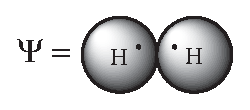
\includegraphics[scale=1]{introduction/figures/heitler.eps}
\caption{Graphical representation of the VB wave function for $\mathrm{H_2}$. The electrons in the two 1$s$ orbitals form a singlet pair.}
\label{ch1.fig.heitler}
\end{figure}
The two determinants together form the VB structure in which the two electrons are spin-coupled into a pair. A graphical representation is shown in Figure \ref{ch1.fig.heitler}. This VB structure represents the Lewis structure $\mathrm{[H^\bullet H^\bullet]}$ for H$_2$, as stressed by Pauling \cite{hllewis}. 

In the years following the introduction of VB, extra versatility was acquired by the expansion of the Valence Bond wave function into multiple structures. For H$_2$ this expansion corresponds to the addition of two ionic structures:
\begin{equation}
\Psi = c_1 (|1s_{A}\overline{1s_{B}}| - |\overline{1s_{A}}1s_{B}|) + c_2 |1s_{A}\overline{1s_{A}}| + c_3 |1s_{B}\overline{1s_{B}}|,
\label{ch1.eq.hlplus}
\end{equation}
in which the third determinant corresponds to the Lewis structure $\mathrm{[H^{-} H^{+}]}$ and the fourth determinant to $\mathrm{[H^{+} H^{-}]}$. A graphical representation is shown in Figure \ref{ch1.fig.heitlerplus}.
\begin{figure}[htp]
\center
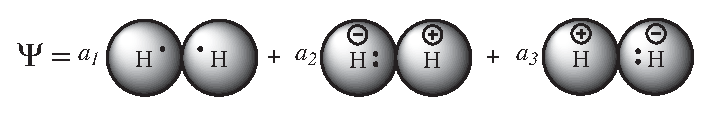
\includegraphics[scale=1]{introduction/figures/heitlerplus.eps}
\caption{Graphical representation of the VB wave function for $\mathrm{H_2}$ with a covalent and two ionic structures. The two bonding electrons are equally shared in the first structure. Both electrons are on the left hydrogen in the second structure and on the right hydrogen in the third structure.}
\label{ch1.fig.heitlerplus}   
\end{figure}
The coefficients $c_1$, $c_2$ and $c_3$ are variationally determined \cite{varia}. The total energy ($E_\mathrm{tot}$) calculated with the $\Psi$ in equation \ref{ch1.eq.hlplus} proved to be lower than the energy calculated with the $\Psi$ in equation \ref{ch1.eq.hl}. In general, for covalent bonds, like H--H, the coefficients $c_2$ and $c_3$ will be non-zero, indicating that they are not merely covalent in nature, but that they also contain some ionic character. This ionic character is caused by the freedom for the electrons to move towards the other atom. The overlap of two singly occupied orbitals on separate atoms or fragments, like the hydrogen atoms mentioned above, can be used as measure for the bond strength. When the two atoms are brought together from infinity to equilibrium distance, the total energy ($E_\mathrm{tot}$) of the molecule decreases as the orbital overlap increases. This suggests that for bonds with ``high overlap'' more energy is required to break it than for bonds with ``low overlap''. This has to be used with caution, though, because at distances shorter than the equilibrium distance, the nuclear repulsion increases so rapidly that this effect will overshadow the still increasing orbital overlap.

The importance (or contribution) of each VB structure to the wave function can be obtained by using the formula of Chirgwin and Coulson \cite{chirgwin}. With their formula weights ($W_j$) can be assigned to the VB structures:
\begin{equation}
W_{j}=\sum_{i} c_{i}c_{j}S_{ij},
\label{ch1.eq.weight}
\end{equation}
in which $S_{ij}$ is the overlap between structure $i$ and $j$ and $c_i$ and $c_j$ are the structure coefficients. This overlap matrix $S_{ij}$ is not necessarily a diagonal matrix, because the structures may overlap, due to the use of non-orthogonal orbitals. For H$_2$ this results in a weight of 0.86 for the covalent $\mathrm{[H^\bullet H^\bullet]}$ structure and 0.07 for both ionic, $\mathrm{[H^{+} H^{-}]}$ and $\mathrm{[H^{-} H^{+}]}$, structures. 

Instead of the homonuclear system H$_2$, one could investigate heteronuclear systems in the same terminology. With the three structures $\mathrm{[A^\bullet B^\bullet]}$, $\mathrm{[A^{+} B^{-}]}$ and $\mathrm{[A^{-} B^{+}]}$ one can study bond polarity and dissociation behavior. This is an application area for VB, as will be exemplified by the following heteronuclear ``molecule''.

The prototype of an electrostatic, or ionic, bond is the one between sodium and chlorine in \mbox{Na--Cl}. As for H--H, a wave function consisting of three structures can be formulated:
\begin{equation}
\Psi = c_1 \cdot \mathrm{[Na^\bullet Cl^\bullet]} + c_2 \cdot \mathrm{[Na^{+} Cl^{-}]} + c_3 \cdot \mathrm{[Na^{-} Cl^{+}]},
\label{ch1.eq.nacl}
\end{equation}
in which determinants comparable to those in equations \ref{ch1.eq.hl} and \ref{ch1.eq.hlplus} have been replaced by Lewis structures for clarity. Throughout this thesis the terms Lewis structure and VB structure are intermixed on several occasions. The reader should be aware that VB structures are not necessarily independent as the pictorial Lewis structures suggest. This is indicated by the possible overlap of the structures in a VB wave function ($S_{ij}$ in equation \ref{ch1.eq.weight}). In practice, VB structures frequently have a non-zero overlap, although they describe different Lewis structures. So, also for the analysis of a chemical bond with a wave function containing only one ionic structure, some covalent character is automatically included. This effect is introduced by the use of non-orthogonal orbitals.

In the $\mathrm{[Na^{+} Cl^{-}]}$ structure, both sodium and chlorine fulfill Lewis' octet rule. The weights of these structures (equation \ref{ch1.eq.weight}) indicate the bond character or polarity of the bond. At equilibrium distance the weight for the $\mathrm{[Na^{+} Cl^{-}]}$ structure is the highest, being 0.75. The covalent $\mathrm{[Na^\bullet Cl^\bullet]}$ structure has a weight of 0.25, while the other ionic structure $\mathrm{[Na^{-} Cl^{+}]}$ does not contribute to the wave function at all. This VB result corresponds to an electrostatic bond. At infinite distance however, the weight for \mbox{$\mathrm{[Na^\bullet Cl^\bullet]}$} equals one, while the weights for the other two structures will be equal to zero. This corresponds to the description of separate neutral atoms.

Another application area is the study of stability in terms of resonance and aromaticity. Resonance is a long known chemical concept, which accounts for stability in molecules, or molecular fragments \cite{whelandbook}. An everyday example is acetic acid (``vinegar'', p$K_\mathrm{a}$~=~4.76 \cite{bruice}). The reason for the acidity of acetic acid is ascribed to the stability of the acetate anion, \textit{viz.} its conjugated base (Figure \ref{ch1.fig.acetic}).
\begin{figure}[ht]
\center
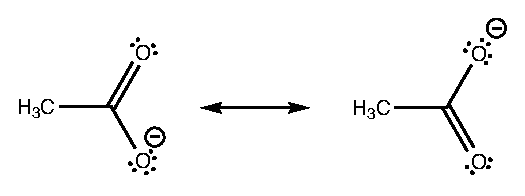
\includegraphics{introduction/figures/acetic.eps}
\caption{The two Lewis resonance structures of the acetate anion, \textit{viz.} the conjugated base of acetic acid.}
\label{ch1.fig.acetic}
\end{figure}
When a proton is abstracted from acetic acid in aqueous environment, the negative charge has to be divided over the acetate anion. After inspection of the Lewis structures in Figure \ref{ch1.fig.acetic} it becomes evident that the negative charge can be positioned on either of the two oxygen atoms, leading to two resonance structures. In contrast, alkanols are known to be very weak acids. For alkanols there is only one resonance structure, in which the negative charge is solely concentrated on the oxygen atom (Figure \ref{ch1.fig.alcohol}). This resonance effect can be explicitly quantified with the Valence Bond method by calculating the Pauling resonance energy $E_\mathrm{res}$ \cite{paulingbook}, which is defined as the difference between the energy of the most stable structure and the energy of the total wave function. 
\begin{figure}[hb]
\center

\includegraphics{introduction/figures/alcohol.eps}
\caption{The deprotonation reaction of methanol (an alkanol; p$K_\mathrm{a}$=15.5 \cite{bruice}). On the right side is the only possible resonance structure.}
\label{ch1.fig.alcohol}
\end{figure}

Resonance energy is often used in discussions on aromaticity. In the 19$^\mathrm{th}$ century Michael Faraday discovered benzene, to which he referred to as bicarburet of hydrogen \cite{faraday,bicarburet}. The molecular weight of 78 suggested that the gross formula was (CH)$_6$. A remarkable property of (CH)$_6$ is that, in contrast to other unsaturated carbon based compounds (such as alkenes), benzene does not give addition products, but only substitution products \cite{bruice}. After several scientists suggested different structural formulae, the planar hexagonal structure of August Kekul\'e \cite{kekule} was generally accepted as the real structure (Figure \ref{ch1.fig.benzene}). 
\begin{figure}[hb]
\center
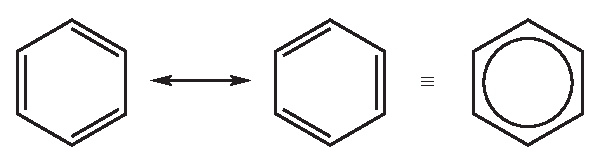
\includegraphics{introduction/figures/benzene.eps}
\caption{The two Kekul\'e resonance structures of benzene (left) and the delocalized electron representation (right).}
\label{ch1.fig.benzene}
\end{figure}

The stability of benzene was ascribed to the delocalization of the 6 $\pi$ electrons, expressed in the resonance between the two Kekul\'e structures.

The Valence Bond wave functions described so far (equations \ref{ch1.eq.hl}, \ref{ch1.eq.hlplus} and \ref{ch1.eq.nacl}) are of the classical type. Modern Valence Bond wave functions do not necessarily describe the bonding between separate atoms, but can also describe the bonding between molecular fragments. On these molecular fragments the orbitals can be expressed as linear combinations of atomic orbitals (AOs) available for that fragment. It is more appropriate to denote these functions as molecular orbitals (MOs), since they can spread over several atoms. 

In modern type Valence Bond wave functions atomic and molecular orbital models can also be mixed. For example, a commonly used VB wave function for benzene consists of complete MO description containing the core (the inner shell AOs, \textit{i.e.} the $1s$ orbitals on carbon) and the $\sigma$ system (the valence shell AOs in the plane of the molecule (X-Y), \textit{i.e.} the $2s$, $2p_x$, $2p_y$ orbitals on carbon and the $1s$ orbitals on hydrogen), while the $\pi$ system is described by atomic $2p_z$ orbitals. The total wave function $\Psi_{tot}$ then becomes an antisymmetrized product of an MO wave function for the core-$\sigma$ system and a VB wave function for the $\pi$ system:
\begin{equation}
\Psi_{tot} = \mathcal{A}(\Psi_{\mathrm{core}-\sigma} \times \Psi_{\pi}),
\label{ch1.eq.prodbenzene}
\end{equation}
in which $\mathcal{A}$ is an anti-symmetrizer. The separation of the core-$\sigma$ and $\pi$ systems does not mean that the two are independent, because the electrons in the core-$\pi$ system will ``feel'' the Coulomb repulsion from the electrons in the $\sigma$ system ($\sigma$-$\pi$ interaction).

In the remainder of this section the three types of Valence Bond wave functions supported by TURTLE \cite{turtle}, the VB module in GAMESS-UK \cite{gamess}, are discussed. These are 1) the Generalized Valence Bond (GVB), 2) the Valence Bond Configuration Interaction (VBCI) and 3) the Valence Bond Self Consistent Field (VBSCF \cite{vbscf1,vbscf2}) models. The latter two types of models are compared to their orthogonal analogues and exemplified with a calculation on benzene. For VBSCF both the delocalized as well as the localized orbital models and the Breathing Orbital Valence Bond (BOVB \cite{bovb1,bovb2,bovb3}) method extension are described. Finally, the Spin-Coupled Valence Bond (SCVB) method \cite{scvb1,scvb2,scvb3} is briefly introduced in this section.

\subsection{Generalized Valence Bond (GVB)}

In the Generalized Valence Bond (GVB) method \cite{jensen,gvb1,gvb2,gvb3,gvb4}, two non-orthogonal orbitals are used to describe a pair of electrons in a bond. Each such pair is coupled to a singlet. Besides these spin-paired singly occupied orbitals, other doubly occupied orbitals may be used. The doubly occupied orbitals and the spin-coupled pairs are chosen orthogonal to each other to reduce the computational effort required. This is called the Strong Orthogonality (SO) condition. The total spin for such a system thus is also singlet. This is known as Perfect Pairing (PP), and is one of the many possible spin coupling schemes, and such two-electron two-orbital pairs are called geminal pairs. A geminal is a wave function for two electrons. 

This type of Valence Bond wave function is used in Chapter \chdissociation\ to generate the geometries on the dissociation curves. For dissociation purposes, a Hartree-Fock wave function does not suffice, since it is not capable of describing a molecule consisting of two radical fragments at large distance from each other.

\subsection{Valence Bond Configuration Interaction (VBCI)}

As the name suggests, there is a strong analogy between the Valence Bond Configuration Interaction Method (VBCI) and Configuration Interaction (section \ref{ch1.sec.ci}). In both cases the orbitals are not optimized in the expansion, but rather only the structure (VB) or CSF (CI) coefficients. A difference between the two is that in the VB case, there is no orthogonality restriction between the orbitals, while in CI the orbitals are orthogonal, leading to more complex calculations in the VB case.

A typical VBCI wave function used in TURTLE consists of several VB structures representing distinctive Lewis structures like the wave function in equation \ref{ch1.eq.hlplus}. Although the bond in H$_2$ is typically covalent in nature, the two ionic structures are included. The effect of the inclusion of the two ionic structures is that the electron on one hydrogen atom gets more freedom to move towards the other hydrogen atom. Even for the covalent bond in H$_2$ this results in a total weight for the ionic structures of 14\% and a lower total energy (\textit{vide supra}) indicating that including these structures improves the wave function.

An example of a VBCI wave function is the wave function for benzene, C$_6$H$_6$, in which the $\pi$ system ($\Psi_{\pi}$) is constructed of atomic $2p_z$ orbitals and the core-$\sigma$ system of 18 doubly occupied orbitals. With 6 $\pi$ electrons, 6 $2p_z$ orbitals and all possible bonding arrangements a wave function consisting of 175 structures can be defined (Figure \ref{ch1.fig.structures2}). 
\begin{figure}[htbp]
\center
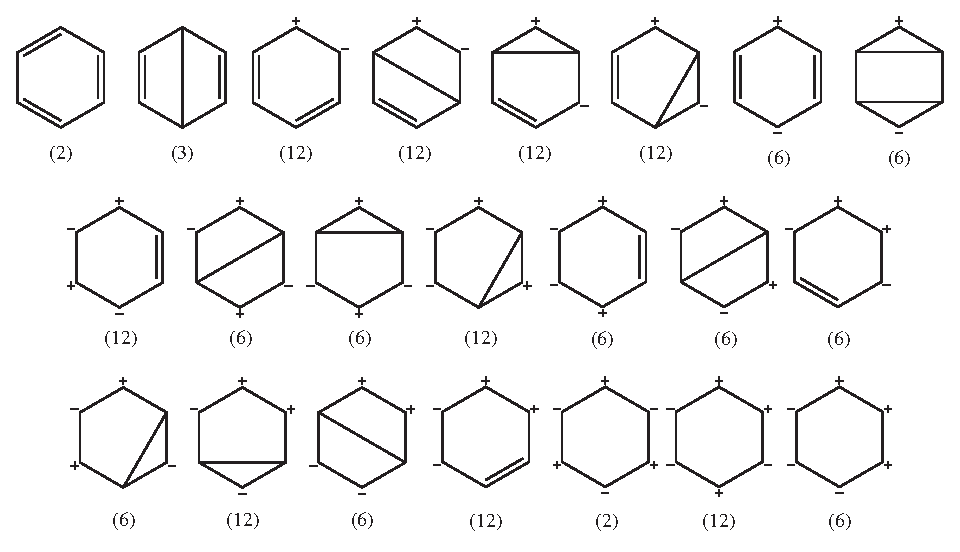
\includegraphics[scale=0.9]{introduction/figures/allstructures.eps}
\caption{The covalent and ionic structures for benzene (with the number of occurrences in brackets): the covalent structures are represented by two Kekul\'e and three Dewar structures. In addition there are 170 ionic structures, giving a total of 175 structures \cite{chembrit}.}
\label{ch1.fig.structures2}
\end{figure}
When all 6 $\pi$ electrons are equally divided over the 6 $2p_z$ orbitals, 5 distinctive bonding arrangements (or spin-couplings) can be made. Two of these are the Kekul\'e structures (Figure \ref{ch1.fig.benzene}). In Figure \ref{ch1.fig.structures2} only one Kekul\'e structure is shown. Beneath it, the number (2) indicates that there are two similar, symmetry related structures in the wave function. The other three bonding arrangements are the Dewar structures (Figure \ref{ch1.fig.structures2}, top row, second from the left), which have a bond across the ring. The other structures in Figure \ref{ch1.fig.structures2} have at least one doubly occupied and one vacant $2p_z$ orbital, resulting in negative and positive charges on the affected carbon atoms, respectively. Several people have used this wave function \cite{vbci175_1,vbci175_2}. Without performing orbital optimizations in the VB model, the total energy ($E_\mathrm{tot}$) for this wave function was found to be lower than that of a single determinant Hartree-Fock wave function with optimized molecular orbitals (MOs). This means that this VBCI wave function has an expectation value for the total energy closer to the best obtainable energy value, \textit{i.e.} the full CI (Configuration Interaction) energy. 

However, the interpretation of the wave function in terms of structure contributions and structure energies proved not  to be trivial. Together with the expected high weights for the Kekul\'{e} structures ($W$ = 0.222 = 2x0.111 \cite{vbci175_2}) and, slightly less, the Dewar structures ($W$ = 0.110 = 3x0.037), also the orthoionic terms (Figure \ref{ch1.fig.structures2}, top row, third from the left) had a high weight ($W$ = 0.251 = 12x0.021). So, looking at single structure contributions, the Kekul\'e structures were most important with a weight of $W$ = 0.111 per structure. However, looking at the total contribution of a structure type, the orthoionic type, with 12 occurrences, were the most important.

To make the wave function more interpretable a VBCI wave function with only the Kekul\'{e} and Dewar structures was used. The results proved to be in line with earlier semi-empirical work on benzene by Craig \cite{craig}. Unfortunately, the energy for this wave function proved to be higher than that of a Hartree-Fock wave function, further from the Full CI energy. Obviously, by excluding the ionic terms, important information for the description of the $\pi$ system was discarded.

In general, an advantage of VBCI is that it can deliver quantitative good results. However, such calculations often require a large number of structures. When many structures have a significant contribution to the wave function the clear Lewis picture may become obscured. Including too few structures on the other hand may lead to a nice interpretable qualitative picture with low quantitative accuracy. 

In the last few years Wu \textit{et al.} have published some articles on VBCI \cite{vbci_wu1,vbci_wu2}. Although they use the same acronym, their interpretation and implementation in Xiamen \cite{xiamen} is different than ours. One of the main goals of using (their) VBCI is the inclusion of electron correlation, \textit{i.e.} the ground state wave function, optimized with VBSCF (see Section \ref{ch1.sec.vbscf}), is expanded with singly (S) and doubly (D) excited states. In a structure with external excitations one or more occupied orbitals are replaced by empty, or virtual, orbitals. Internal excitations are excitations to orbitals which are vacant in some structures. An example of such an excitation is from $\mathrm{[H^\bullet H^\bullet]}$ to $\mathrm{[H^{+} H^{-}]}$, \textit{i.e.} from $1s_A$ to $1s_B$ once for $\alpha$ and once for $\beta$ spin. Wu defines three levels of expansion: in VBCI(S,S) only singly excited structures are involved. In VBCI(D,S) the active shell, \textit{e.g.} the orbitals in $\Psi_{\pi}$ in benzene (equation \ref{ch1.eq.prodbenzene}), is treated by single and double excitations, whereas the inactive shell, \textit{e.g.} $\Psi_{\mathrm{core}-\sigma}$, is expanded with single excitations only. Also included in this level are double excitations which consist of a single excitation from each shell. In VBCI(D,D) single and double excitations are involved for both active and inactive electrons.

\subsection{\label{ch1.sec.vbscf}Valence Bond Self Consistent Field (VBSCF)}

Like in VBCI, the wave function in VBSCF is expressed in VB structures. However, in contrast to VBCI, the coefficients of the structures \textit{and} of the orbitals are optimized. This is analogous to the Multi Configuration Self Consistent Field method (MCSCF) (section \ref{ch1.sec.mcscf}). A VBSCF wave function is  expressed in structures, which are the non-orthogonal equivalent of the Configuration State Functions (CSFs) in MCSCF.  Two major differences are that both bonding \textit{and} anti-bonding orbitals occur in CSFs and that the molecular orbitals (MOs) are chosen orthogonal in MCSCF.

In analogy with MCSCF, in VBSCF the Super CI method \cite{superci1,superci2}, in which the wave function is expanded with singly excited structures, can be used. For VBSCF, however, the overlap matrix between the structures ($\mathbf{S}$) enter the equation (compare with MCSCF in equation \ref{ch1.eq.geig}). Likewise, the  Brillouin vector is determined by solving the generalized eigenvalue problem:
\begin{equation}
[\mathbf{H}-E_b\mathbf{S}] \cdot \mathbf{b} = 0,
\label{ch1.eq.geigvb}
\end{equation}
in which $\mathbf{H}$ and $\mathbf{S}$ are the Hamiltonian and metric in the basis of the ground state and the singly excited states ($\Psi_0$ and the $\Psi_{ia}$'s). $E_b$ is the lowest eigenvalue and $\mathbf{b}$ is the corresponding eigenvector. With the elements of $\mathbf{b}$ the orbitals are updated (for details  \textit{cf.} Chapter \chorbopt), like in equation \ref{ch1.eq.brillouin}.

Cooper, Gerratt and Raimondi investigated benzene with a VB wave function in which they optimized the orbitals \cite{nature}. In their wave function the core-$\sigma$ part was frozen, or kept constant, while the singly occupied $\pi$ orbitals were expressed as linear combinations of the 6 atomic $2p_z$ orbitals. This meant that the $\pi$ orbitals could spread out over the whole $\pi$ system during the optimization process. As Cooper showed, the advantage of the use of a VB wave function with optimized orbitals is that it gives good quantitative results with only a few VB structures: addition of the 170 ionic structures (Figure \ref{ch1.fig.structures2}) to this wave function only resulted in a small energy lowering. Although the orbitals were allowed to spread over the whole $\pi$ system, the orbitals remained centered on the carbon atoms with tails on the neighboring carbons (Figure \ref{ch1.fig6}, top). 
\begin{figure}[htbp]
\center
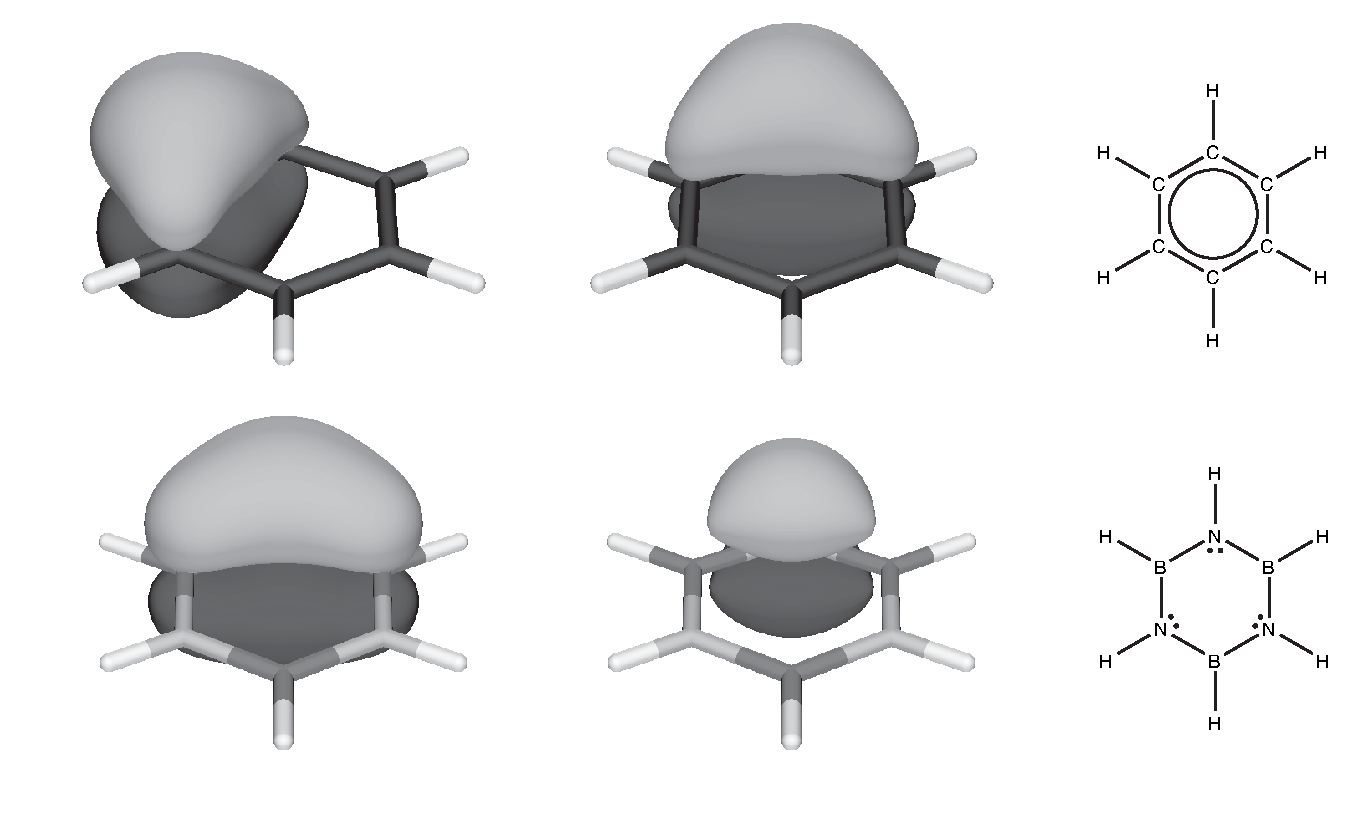
\includegraphics[scale=0.5]{introduction/figures/figure6.eps}
\caption{A set of singly occupied $p$ orbitals on benzene (C$_6$H$_6$, top) and on borazine (B$_3$N$_3$H$_6$, bottom). In these orbital plots the boron atoms are dark colored and the nitrogen atoms light.}
\label{ch1.fig6}
\end{figure}
The orbitals in these plots, made with Molden \cite{molden}, are taken from a VBSCF calculation (\textit{cf.} Chapter \chinorganic). They are, however, equivalent with the contour plots of the orbitals as published with the Spin Coupled Valence Bond (SCVB) method (see Section \ref{ch1.sec.scvb}) by Cooper \textit{et al.} in Nature \cite{nature}.

A molecule that is iso-electronic with benzene and also has a planar hexagonal structure is borazine (see the structural formulae on the right hand side in Figure \ref{ch1.fig6}: top - benzene; bottom - borazine). The distribution of the 6 $\pi$ electrons, however, is rather different. In benzene, each carbon atom contributes one $p$ electron, while in borazine only the nitrogen atoms contribute two $p$ electrons each. VBSCF calculations with initial atomic $p$ orbitals on each atom of both hexagonal molecules show that the $p$ orbitals remain more or less centered on the initial carbon atom in the case of benzene,  while in the case of borazine an atomic $p$ orbital, which originated on a boron atom, migrated to a neighboring nitrogen atom (with tails remaining on the boron atoms), forming a (localized) lone-pair description with the $p$ orbital already present there (Figure \ref{ch1.fig6}, bottom).

In some cases, due to the increased flexibility of the wave function, the orbitals might no longer be centered on an atom or a bond, but spread out over the whole molecule. In those situations, the interpretability is obscured. In a normal VBSCF calculation all MOs are expressed in all AOs. As a consequence, MOs can completely migrate from one atom to another atom, or fragment during orbital optimization and become \textit{delocalized}. In TURTLE it is possible to specify the AOs available for each MO. During the optimization process these MOs are not allowed to mix in AOs not initially specified. This keeps the MOs \textit{localized}. 

An example of a molecule which is constructed from two fragments with \textit{localized} orbitals is CpSiH (Figure \ref{ch1.fig7}). To investigate the type of bonding between the main group metal Si and the cyclopentadienyl (Cp) ring, two covalent ([Cp$^\bullet$SiH$^\bullet$]) structures and one ionic ([Cp$^{-}$SiH$^{+}$]) structure were defined. In these structures the orbitals on the Cp ring were completely separated from the orbitals on the SiH group.
\begin{figure}[htbp]
\center
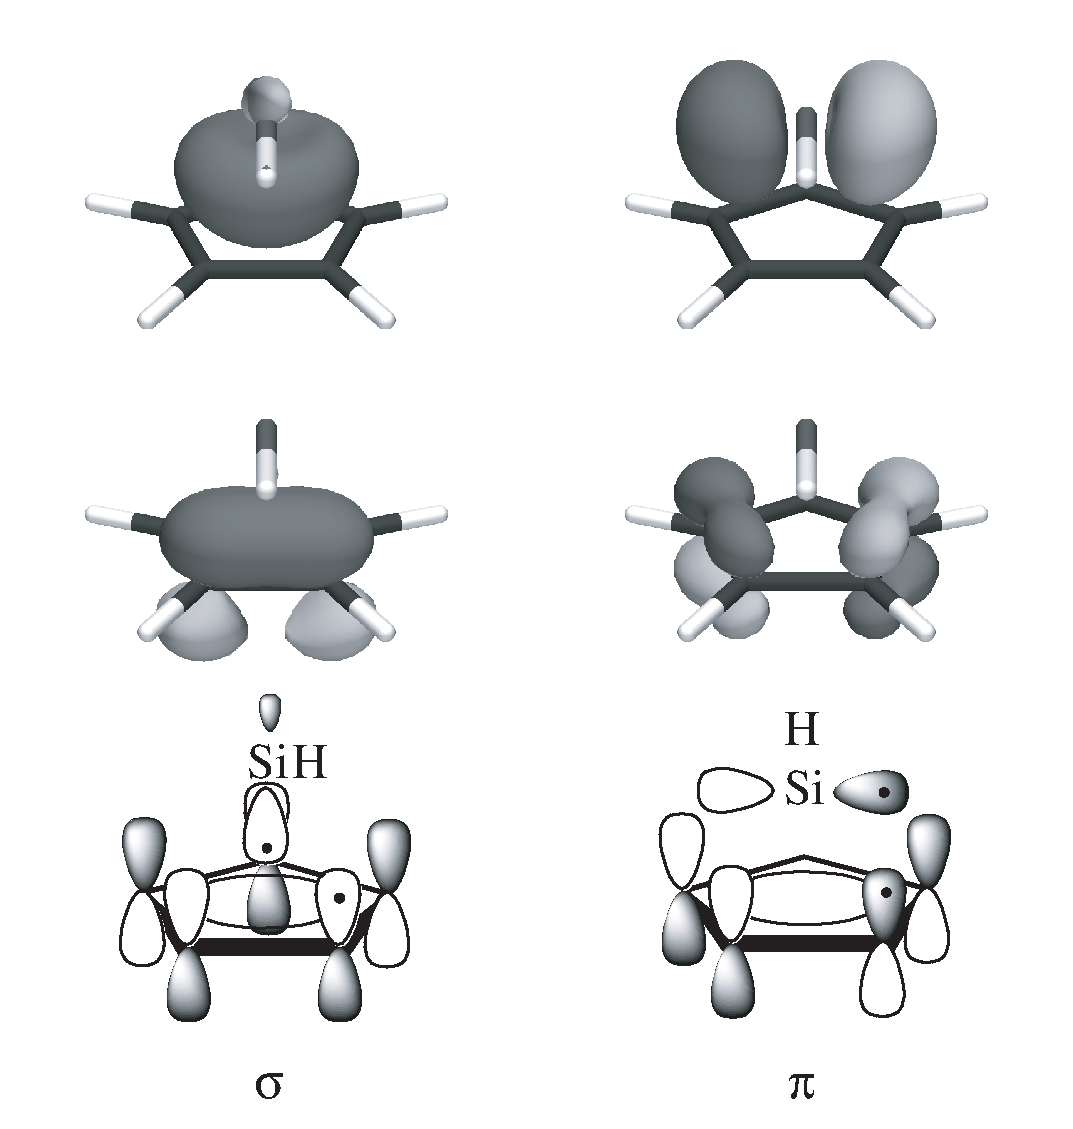
\includegraphics[scale=0.5]{introduction/figures/figure7.eps}
\caption{On the bottom the covalent bond structures are shown, on the left is the $\sigma$ description and on the right is the $\pi$ description. The actual resulting bonding orbitals from the local VBSCF calculation on SiH and Cp are shown on top and in the middle, respectively.}
\label{ch1.fig7}
\end{figure}
The two covalent structures are shown on the bottom in Figure \ref{ch1.fig7}. On the left is the $\sigma$ type bond and on the right a $\pi$ type bond. Both bonds consist of an electron pair of which one electron is located on the siliconhydride part (top) and one on the cyclopentadienyl ring (middle). With the localized orbital model the resulting VB orbitals (top and middle) remain clearly belonging to the separate fragments. 

A drawback of local VBSCF, however, is that it is not very suitable as a quantitative tool: mostly, the total VB energy is higher than for a VBCI calculation with many structures or a delocal VBSCF calculation. And in some cases the use of localized orbitals can even be too restrictive, which might lead to the prediction of a wrong geometry. For example, a calculation on cyclobutadiene with the local VBSCF model \cite{cyclobutt} has shown that the localization of the $p$ orbitals results in a square geometry, rather than the generally accepted rectangular geometry (Figure \ref{ch1.fig.butadiene}) \cite{arnold}. 
\begin{figure}[htp]
\center
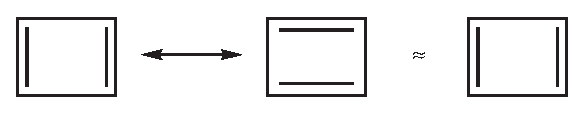
\includegraphics{introduction/figures/butadiene.eps}
\caption{The two Kekul\'e-like resonance structures of cyclobutadiene (left) which is approximately equal to the structure on the right.}
\label{ch1.fig.butadiene}
\end{figure}
From H\"{u}ckel's $\pi$ electron rule \cite{huckel2,huckel4}, it is expected that planar hydrocarbons ((CH)$_n$) with $4n+2$ $\pi$ electrons are aromatic, while molecules with $4n$ $\pi$ electrons are anti-aromatic. One of the properties of aromatic molecules is their bond length equalization, like in benzene (Figure \ref{ch1.fig.benzene}). For anti-aromatic molecules the double bonds are shorter than the single bonds. The reason for the bond length equilibration for C$_4$H$_4$ in the local VBSCF model is that the $\pi$ bonds are weaker because they have less overlap due to the localization \cite{cyclobutt}. A calculation with the delocal model results in the rectangular geometry \cite{cyclobutt}. Furthermore, in this delocal wave function only one Kekul\'{e}-like structure contributed mainly to the wave function (Figure \ref{ch1.fig.butadiene}, left), resulting in a negligible resonance energy.

In the VB wave functions described so far there is only \textit{one} set of orbitals. In the previous benzene examples (Figure \ref{ch1.fig.structures2}) all structures used the same 6 $2p_z$ orbitals. In the 1990s Hiberty \textit{et al.} introduced the Breathing Orbital Valence Bond method (BOVB). In a BOVB wave function \textit{each structure} has its \textit{own set of orbitals}. For F$_2$, with the structures $\mathrm{[F^\bullet F^\bullet]}$, $\mathrm{[F^{+} F^{-}]}$ and $\mathrm{[F^{-} F^{+}]}$, this means that F$^\bullet$, F$^{-}$ and F$^{+}$ have different orbitals. So, the covalent structure has orbitals optimized for neutral atoms, while the ionic structure has orbitals optimized for charged atoms, which, from an electrostatic point of view, corresponds more to reality than both structures having the same, mostly an average between the two extremes, set of orbitals. The higher versatility of the BOVB method compared to plain VBSCF is reflected in the lower expectation values of the energy, although at cost. Because orbitals in different structures might resemble each other much, \textit{i.e.} have a large overlap, dependencies in the orbital basis can occur, which leads to difficult convergence or no convergence at all.

\subsection{\label{ch1.sec.scvb}Spin-Coupled Valence Bond (SCVB)}
Cooper, Gerratt and Raimondi have developed the Spin-Coupled Valence Bond (SCVB) method that uses a single reference configuration \cite{scvb1,scvb2,scvb3}. This reference configuration contains doubly and singly occupied orbitals. For the singly occupied orbitals \textit{all} spin-couplings are taken into account. A special form of SCVB is the Complete Active Space Valence Bond (CASVB). As the name of the latter suggests, in CASVB all possible excited structures are generated in the active space. This corresponds to a full CI in the active space. Wave functions of the CAS type are invariant to general transformations and hence the CASVB wave function can be transformed to an (orthogonal) CASSCF wave function. This wave function is optimized (see section \ref{ch1.sec.mcscf}) and transformed back into the CASVB wave function \cite{thor1,thor2,thor3,thor4}.

SCVB is equivalent with the VBSCF method described in the previous subsection. That is, if in the VBSCF all possible spin-couplings are taken into account. In that case, the expectation value for the total energy ($E_\mathrm{tot}$) will be the same for the same basis set.

\section{Methods Using Extended, or Perturbed, Hamilton Operators}
In this thesis, the molecules described are not only studied by solving the Schr\"{o}dinger equation (equation \ref{ch1.eq.hpsi}) with the standard Hamilton operator (equation \ref{ch1.eq.htotal}), but with extended, or perturbated, Hamiltonians as well. With these operators additional characteristics, like solvation  (Chapter \chdissociation) and  magnetically induced ring currents (Chapters \chhuckel, \chinorganic\  and \chindacene), can be studied. 

\subsection{\label{ch1.sec.solv}Solvation}
In computational chemistry, the methods for evaluating solvent effects can be divided into two types: those describing the individual solvent molecules and those that treat the solvent as a continuous medium \cite{jensen}. In continuum models, like the Polarizable Continuum Model (PCM) \cite{pcm1,pcm2}, the solvent is considered to be a uniform polarizable medium with a dielectric constant of $\epsilon$. The solute \textbf{M} is placed in a suitably shaped hole in the medium (Figure \ref{ch1.fig.continuum}).
\begin{figure}[hb]
\center
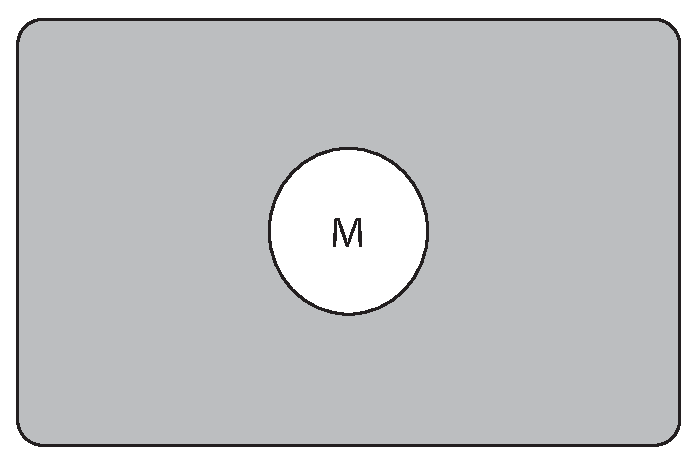
\includegraphics[scale=0.6]{introduction/figures/continuum.eps}
\caption{The solute (\textbf{M}) placed in a suitably shaped hole (white circle), placed in a medium (gray area).}
\label{ch1.fig.continuum}
\end{figure}
In Chapter \chdissociation\ the effect of water is mimicked with a value for $\epsilon$ of 78.5. For the holes around the atoms, spheres are chosen. As an estimate for the size, the van der Waals radii of the atoms were taken, scaled by 1.20. The cavity around the molecules therefore becomes shaped liked the molecules themselves. 

For a (polar) molecule \textbf{M}, the calculated electric moments induce charges in the dielectric medium. In turn, this medium acts back on the molecule, causing the wave function to respond. This response changes the electric moments. The interaction with the solvent model is therefore calculated via an iterative procedure called the Self-Consistent Reaction Field (SCRF) method \cite{jensen}.

In SCRF, the Hamiltonian is extended with the potential $\phi_\sigma$ from the surface charge given by the molecular charge distribution:
\begin{equation}
\begin{split}
\mathbf{H}&=\mathbf{H}_0 + \phi_\sigma,\\
\phi_\sigma(\mathbf{r})&=\int\frac{\sigma(\mathbf{r}_\mathrm{s})}{|\mathbf{r}-\mathbf{r}_\mathrm{s}|}\mathbf{dr}_\mathrm{s},\\
\end{split}
%Deze vergelijking komt uit Jensen, vergelijking 14.64 :-)
\end{equation}
in which $\mathbf{H}$ is the total Hamiltonian, $\mathbf{H}_0$ the Hamiltonian for the free molecule \textbf{M} and $\phi_\sigma(\mathbf{r})$ the surface charge being the integral over the charges $\sigma(\mathbf{r}_\mathrm{s})$ at points $\mathbf{r}_\mathrm{s}$. Since the change in the wave function results in an updated $\phi_\sigma$, the optimization of the system is iterative in nature.

\subsection{\label{ch1.sec.magnet}Magnetically Induced Ring Currents}
Molecules react differently to an external magnetic field. In benzene, for example, the center of the ring is shielded, while the edges of the molecule are deshielded. Benzene, like other cyclic conjugated aromatic systems, have the ability to sustain a diaptropic ring current \cite{nics1} (see Figure \ref{ch1.fig.ringcurrent}).
\begin{figure}[htp]
\center
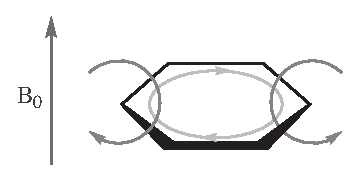
\includegraphics{introduction/figures/ringcurrent.eps}
\caption{A diagram of an aromatic ring current. $\mathrm{B_0}$ is the applied magnetic field, the up-arrow indicating its direction. The arrows in the plane of the atoms shows the direction of the ring current, and the two rings with arrows perpendicular to the C$_6$ ring show the direction of the induced magnetic field. Note that the direction of the current is the opposite of the direction of movement of the ($\pi$) electrons.}
\label{ch1.fig.ringcurrent}
\end{figure}
If a magnetic field is directed perpendicular to the plane of an aromatic system, like benzene, a ring current is induced in the delocalized $\pi$ electrons of the aromatic ring, since these $\pi$ electrons are free to circulate, and hence obey Amp\`{e}re's Law. On the other hand, antiaromatic systems sustain paratropic ring currents despite their localized, destabilized structure \cite{nics1}.

Schleyer \textit{et al.} have proposed the use of absolute magnetic shieldings \cite{nics1,nics2,nics3,nics4}, computed at the ring centers with quantum chemical programs, as a aromaticity/antiaromaticity criterion. To correspond to the familiar NMR chemical shift conventon, the signs of the computed values are reversed. Negative ``nuclues-independent chemical shifts'' (NICSs) denote aromaticity, while positive values indecate antiaromaticity \cite{nics1}.

In the past, several methods have been developed to study ring currents. A reappearing question for these has been: what is the best position to choose the gauge, \textit{i.e.} the formal ``center of rotation''? To study the ring current in the $\pi$ system of a planar cyclic conjugated system, would that be the center of the ring? Methods that use a discrete distributions of origins, rather than a one center gauge, include the Individual Gauge Localized Orbitals (IGLO) \cite{iglo1,iglo2} and the Gauge-Including Atomic Orbitals (GIAO) methods \cite{giao}. Keith and Bader suggested that the origin distribution could be a continuous function with the induced current density at each point in space computed with respect to the origin of the vector potential \cite{keithbader}. This led to the development of the equivalent Continuous Set of Gauge Transformations (CSGT) \cite{keithbader} and Continuous Transformation of the Origin of the Current Density (CTOCD) \cite{ctocd} methods.

For a molecule in a static, uniform, magnetic field, the current density distribution does not depend on the choice of the gauge \cite{ipso1}. For the contributions per orbital, the choice of the gauge does have influence. This may be the reason that for studies with one center gauge calculations orbital contributions have seldom been used. The CTOCD method does not have this restriction and the current density can be split in contributions per orbital.

The first order current density distribution ($\mathbf{j}(\mathbf{r})$) consists of a diamagnetic and a paramagnetic contribution and is the sum of current density contributions for each orbital ($\mathbf{j}_n(\mathbf{r})$) \cite{ipso1}:
\begin{equation}
\begin{split}
\mathbf{j}(\mathbf{r}) &= \mathbf{j}^{(\mathrm{d})}(\mathbf{r}) +\mathbf{j}^{(\mathrm{p})}(\mathbf{r}) \\
&= \sum_n \mathbf{j}_n(\mathbf{r}),
\end{split}
\label{ch1.eq.jtot}
\end{equation}
in which $n$ runs over all orbitals.  $\mathbf{j}^{(\mathrm{d})}(\mathbf{r})$ and $\mathbf{j}^{(\mathrm{p})}(\mathbf{r})$ are the diamagnetic and paramagnetic contributions. $\mathbf{j}(\mathbf{r})$ can be expressed in magnetic field, charge density, the ground state wave function and its first order perturbation correction:
\begin{equation}
\mathbf{j}(\mathbf{r}) = \frac{e}{2m_e} \mathbf{B} \times (\mathbf{r}-\mathbf{d}) \rho_0 (\mathbf{r}) + \frac{ie{\hbar}N}{m_e} \int [ \Psi_0 \nabla \Psi^{(1)}_0 - \Psi^{(1)}_0 \nabla \Psi_0 ] d\tau',
\label{ch1.eq.jtotlong}
\end{equation}
in which $\mathbf{B}$ is the magnetic field, $\mathbf{r}$ the coordinates, $\mathbf{d}$ the origin of the vector potential, and $\rho_0$ the charge density. $\Psi_0$ is the wave function that describes the ground state and $\Psi^{(1)}_0$ is the first order perturbation correction to the wave function.

The current density for orbital $n$, $\mathbf{j}_{n}(\mathbf{r})$, is:
\begin{equation}
\mathbf{j}_{n}(\mathbf{r}) = \frac{e^2}{2m_{e}}\mathbf{B} \times (\mathbf{r}-\mathbf{d})\psi_{n}^2 + \frac{ie\hbar}{m_{e}} [ \psi_{n} \nabla \psi_{n}^{(1)} - \psi_{n}^{(1)} \nabla \psi_{n} ],
\label{ch1.eq.jperorbital}
\end{equation}
in which $\psi_{n}$ and $\psi_{n}^{(1)}$ are the orbital and its first order correction, respectively. The first order correction $\psi_{n}^{(1)}$ is:
\begin{equation}
\begin{split}
\psi_{n}^{(1)}(\mathbf{r;d}) = - \frac{e}{2m_{e}} &\left [ \sum_{p>N/2} \psi_{p}(\mathbf{r})\frac{\left <\psi_{p}|\mathbf{\hat{l}}(\mathbf{0})|\psi_{n}\right >}{\epsilon_{p}-\epsilon_{n}} \right ] \cdot \mathbf{B} + \\
&\frac{e}{2m_{e}} \left [ \mathbf{d} \times \sum_{p>N/2} \psi_{p}(\mathbf{r})\frac{\left <\psi_{p}|\mathbf{\hat{p}}|\psi_{n}\right >}{\epsilon_{p}-\epsilon_{n}} \right ] \cdot \mathbf{B},
\end{split}
\label{ch1.eq.psi_n_1}
\end{equation}
in which $\psi_{n}$ is an orbital from the $N/2$ doubly occupied orbitals. Index $p$ runs over all non occupied (virtual) orbitals. $\epsilon_{n}$ and $\epsilon_{p}$ are the orbital energies of the occupied and virtual orbitals, respectively. $\mathbf{\hat{l}}(\mathbf{0})$ is the angular momentum operator about the origin of coordinates, $\mathbf{d}$ is the displacement vector from the origin and $\mathbf{\hat{p}}$ is the linear momentum operator.

In the CTOCD-\textit{DZ} formalism, $\mathbf{j}^{(\mathrm{d})}(\mathbf{r})$ is set to zero by choosing each point $\mathbf{r}$ as its own origin ($\mathbf{r}$ is then equal to $\mathbf{d}$). This reduces equation \ref{ch1.eq.jtotlong} to:
\begin{equation}
\mathbf{j}(\mathbf{r}) = \frac{ie{\hbar}N}{m_e} \int [ \Psi_0 \nabla \Psi^{(1)}_0 - \Psi^{(1)}_0 \nabla \Psi_0 ] d\tau',
\label{ch1.eq.jtotdz}
\end{equation}
a sum over states. With this equation, a classical diamagnetic response has been included into a single description in which diamagnetic \textit{and} paramagnetic effects can be interpreted in terms of the accessibility of excited states. As is explained in detail in reference \cite{ipso1}, the translational excitations (from the linear momentum operator) give rise to diamagnetic ring current contributions, while the rotational excitations (from the angular momentum operator) give rise to paramagnetic ring current contributions. A first striking observation with the CTOCD-\textit{DZ} method was that only 4 $\pi$ electrons are responsible for the diatropic ring current of aromatic ($4n+2$)-electron monocycles \cite{ipso1}. In Figure \ref{ch1.fig.orbital_scheme} it can be seen that the diamagnetic ring current in benzene (a) is caused by translational excitations, while the paramagnetic ring current in planar cyclooctatetraene (b) is caused by rotational excitations.
\begin{figure}[hb]
\center
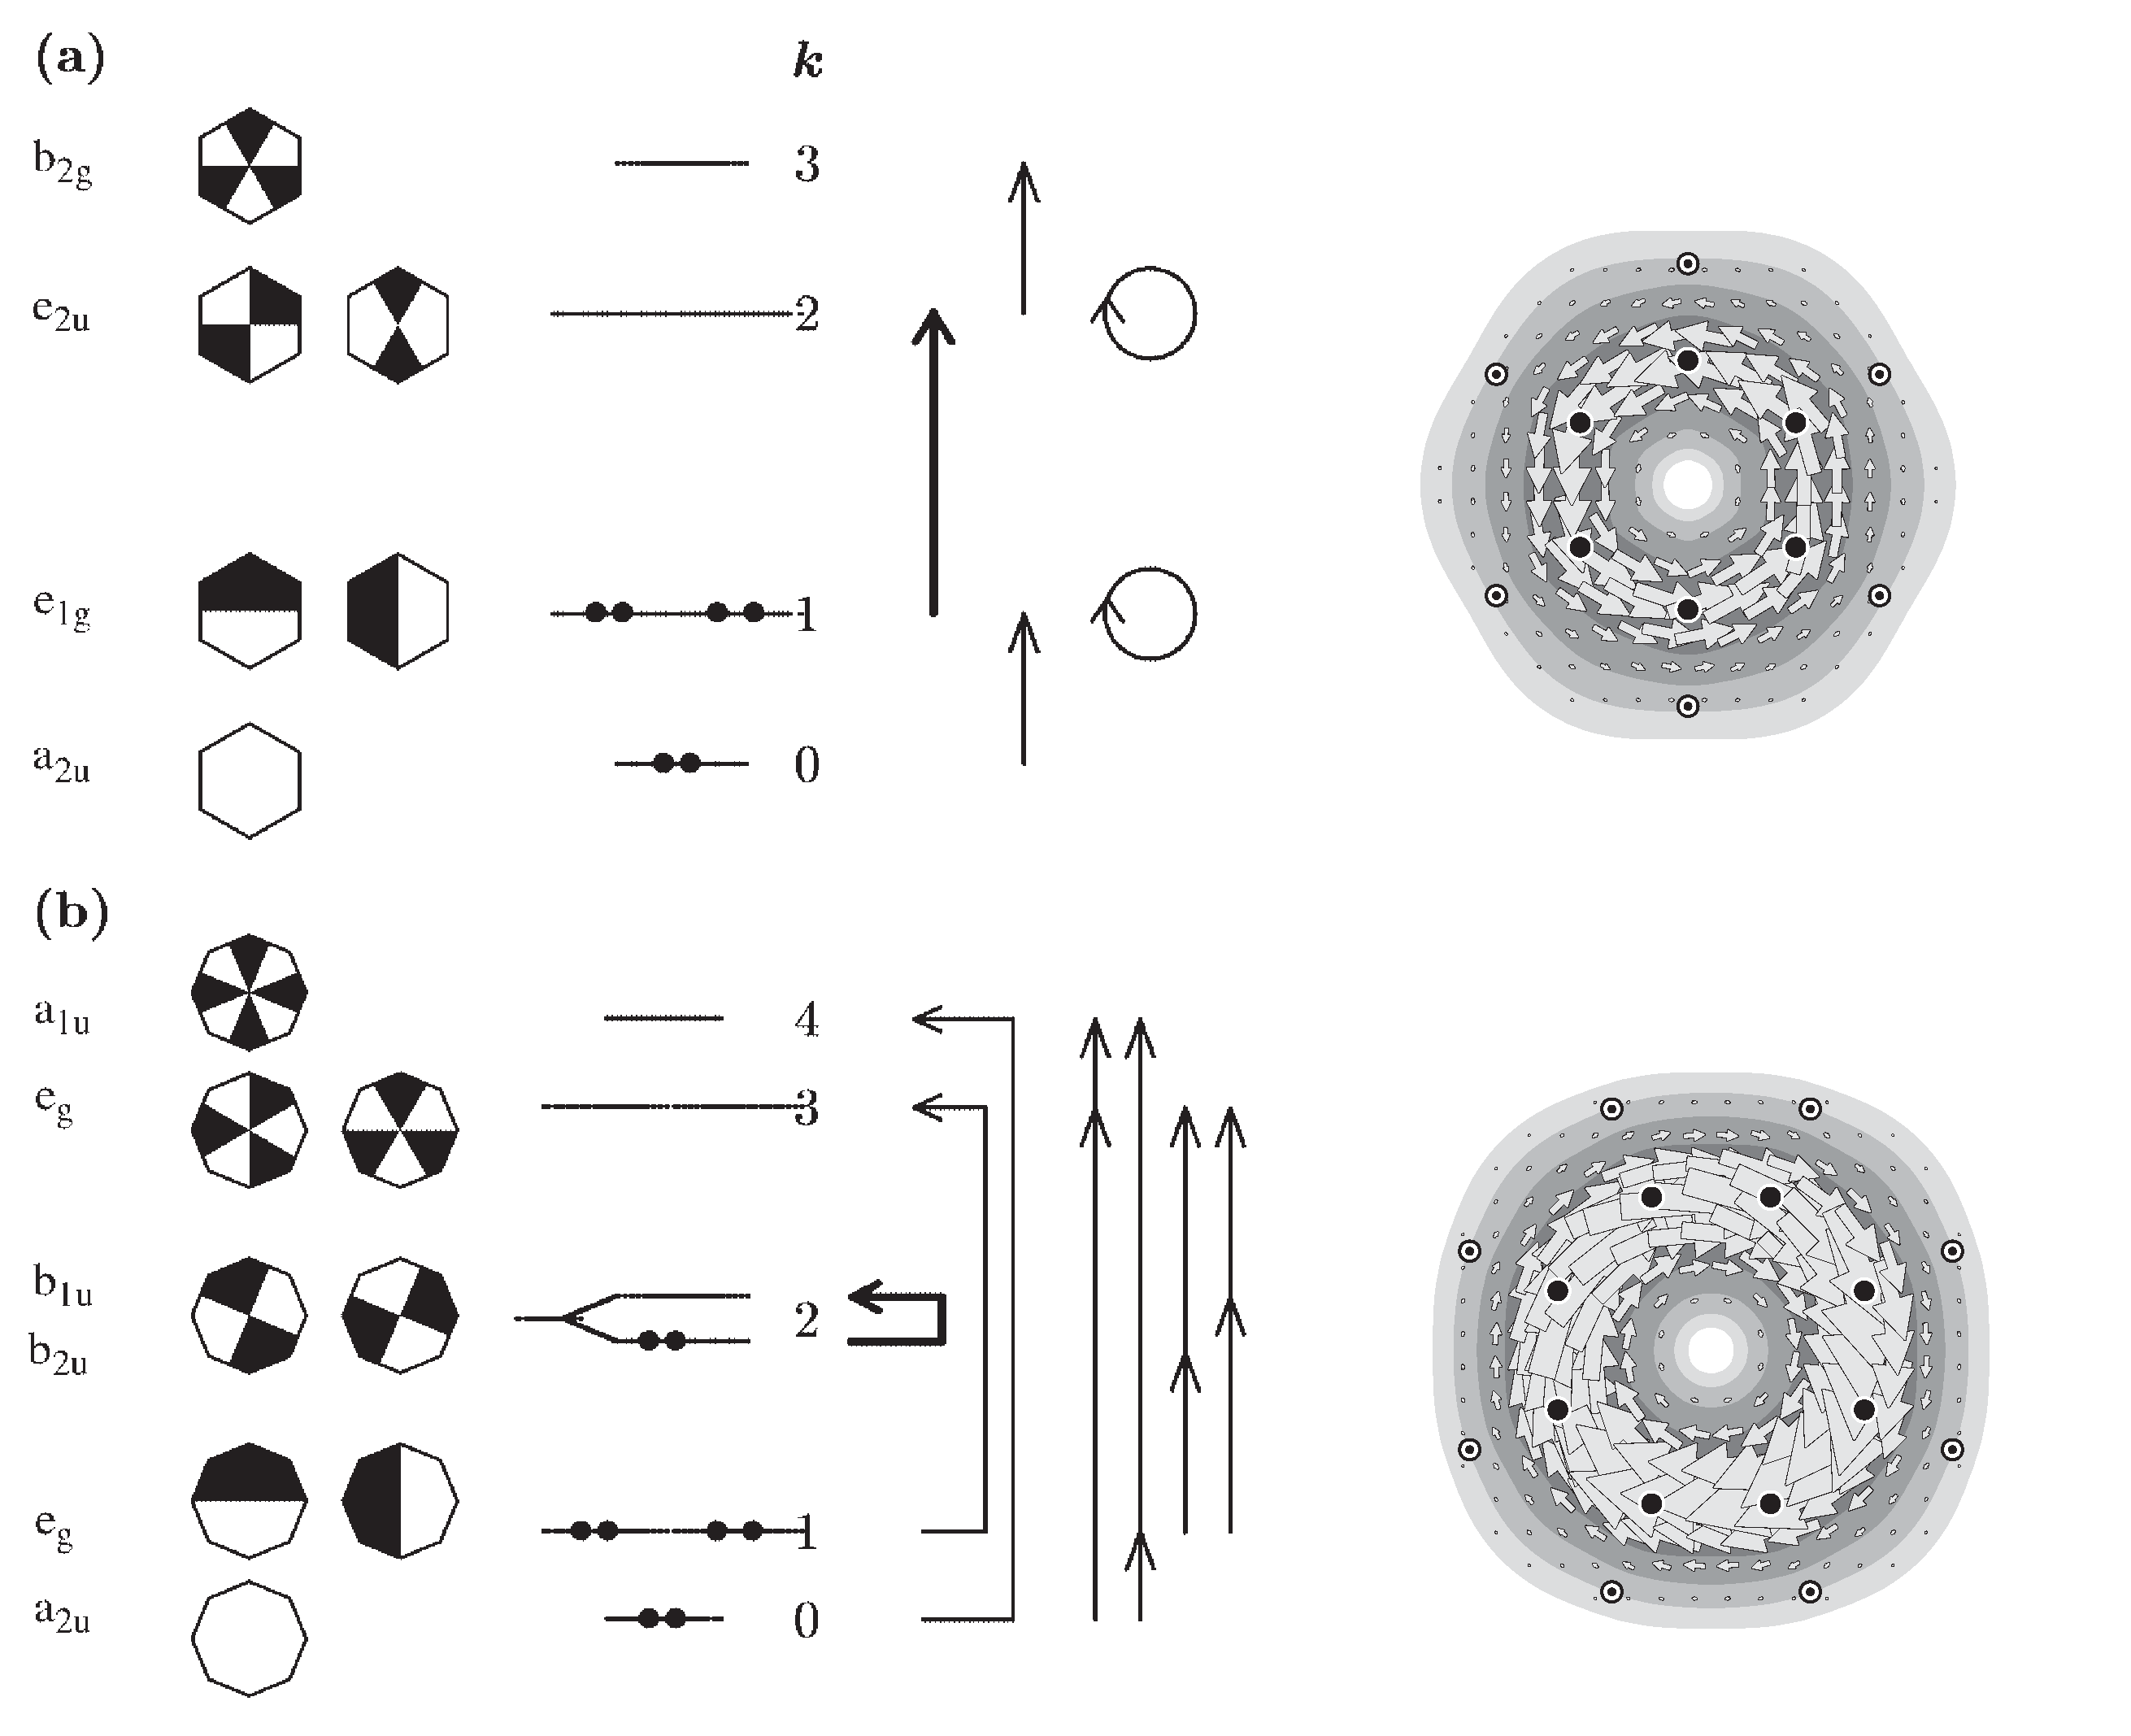
\includegraphics[scale=0.21]{introduction/figures/orbital_scheme.eps}
\caption{Orbital energy scheme for (a) benzene ($D_\mathrm{6h}$) and (b) planar cyclooctatetraene ($D_\mathrm{4h}$), showing symmetries, nodal characteristics, occupancies and \textit{k} values. Possible transitions are indicated by straight (translational) and bent (rotational) arrows (Figure taken from reference \cite{ipso2}). On the left hand side the HOMO-LUMO transition is indicated by bold arrows. On the right hand side, the contribution of HOMO to the total current density is shown.}
\label{ch1.fig.orbital_scheme}
\end{figure}
The HOMO-LUMO transitions are shown by bold arrows. A straight arrow indicates a translational transition (in the case of benzene, (a)), while a bent arrow indicates a rotational transition (in the case of cyclooctatetraene (b)). On the right hand side in the figure, the induced ring current plots are shown for the HOMO-LUMO transitions in both molecules. While for benzene a diatropic (counter clockwise) induced ring current is descernible, a paratropic (clockwise) induced ring current is visible in the plot for (planar) cyclooctatetraene. This clear distinction between aromatic and anti-aromatic molecules is used throughout the last three chapters of this thesis.

\section{Overview of this Thesis}

This thesis consists of three parts: methodology (Chapter \chorbopt), assessment of complex chemical bonding, such as bond making and breaking of dative bonds and bonds with different $\eta$-hapticities (Chapters \chdissociation\ and \chcyclopentadienyl), and aromaticity (Chapters \chhuckel, \chinorganic\ and~\chindacene).

As mentioned earlier, the orbitals in a VB wave function can be optimized with \mbox{VBSCF}. One of the optimization methods is Super CI. Within this method, the VB wave function is extended with all possible singly excited structures. These singly excited structures contain 1-2 times the number of determinants in the ground state wave function. Besides, due to the non-orthogonality, first and second order cofactors, which are signed subdeterminants with orbital overlaps, need to be evaluated.

In Chapter \chorbopt\ the possibilities to bypass these singly excited structures and cofactors are analyzed. In MCSCF, Fock matrices have been used for the optimization of doubly occupied orbitals \cite{roos1,roos2}. The analogy between MCSCF and VBSCF, as explained in Section \ref{ch1.sec.vbscf}, justifies a close look at the possible use of a Fock operator in VBSCF. In this chapter the applicability of Fock matrices for the optimization of orbitals in VBSCF is analyzed. Besides, several improvements on the earlier implemented approximated Newton-Raphson technique \cite{koos1} will be presented. The chapter is concluded with some test calculations for which the speed-up factors are compared.

The dissociation behavior of chemical bonds is influenced by the surrounding medium. In Chapter \chdissociation\ this influence is analyzed by comparing the dissociation behavior of four chlorine containing compounds both in the gas-phase and in solution. The molecules are chloromethane, \textit{tert}-butylchloride, chlorosilane and trimethylsilylchloride (Figure \ref{ch1.fig.structures1} in which M = C or Si and R = H or CH$_3$).
\begin{figure}[htbp]
\center
\includegraphics{introduction/figures/structures.eps}
\caption{The total wave function is a combination of three Lewis structures \textbf{a}, \textbf{b} and \textbf{c}, in which M = C or Si and R = H or CH$_3$.}
\label{ch1.fig.structures1}
\end{figure}
The M--Cl bond  is stretched and for several bond lengths the total VB energy and the energy of the separate covalent and ionic structures is calculated. At large distances only the covalent structure (Figure \ref{ch1.fig.structures1}, structure \textbf{a}) contributes to the wave function for the gas-phase.

With PCM switched on (see Section \ref{ch1.sec.solv}), \textit{tert}-butylchloride, chlorosilane and trimethylsilylchloride dissociate in ions, \textit{i.e.} at large distances only the ionic structure (Figure \ref{ch1.fig.structures1}, structure \textbf{b}) contributes to the wave function.  Chloromethane is hardly influenced by the solvating medium. At large distances the covalent structure remains the most important for this molecule.  

The cyclopentadienyl anion has 6 $\pi$ electrons and fulfills the 4$n$+2 H\"{u}ckel rule for $\pi$ electrons. Although the cyclopentadienyl moiety is frequently used as a ligand in organometallic chemistry (\textit{cf.} ferrocene) details about the actual bond between the metal atom and the ligands are scarce \cite{budzelaar}. In Chapter \chcyclopentadienyl\ the bonding of main-group metal hydrides to a cyclopentadienyl ring is, for which the covalent structures were already shown in Figure \ref{ch1.fig7}, investigated in terms of contributions of VB structures, describing $\sigma$, $\pi$ and ionic bonding (Figure \ref{ch1.fig.mhydride}).
\begin{figure}[ht]
\center
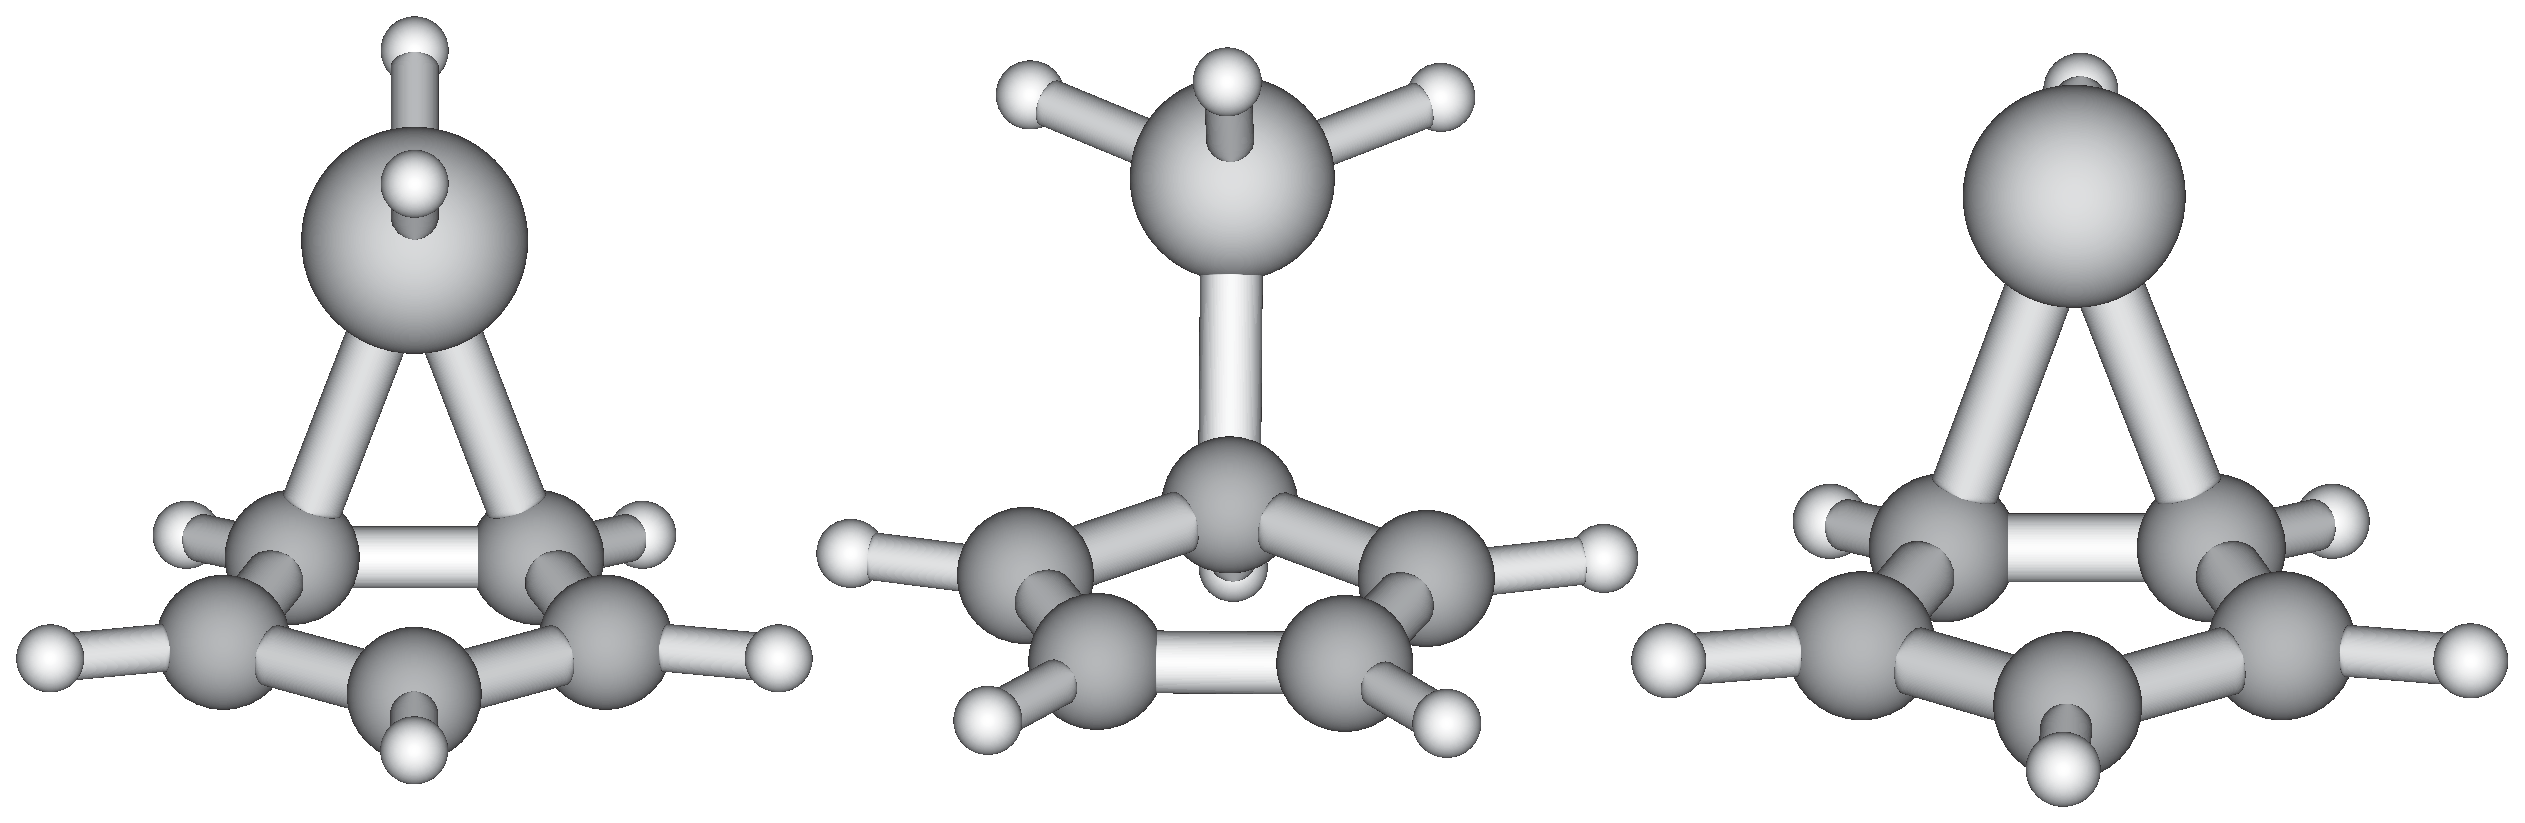
\includegraphics[scale=0.3]{introduction/figures/mhydride.eps}
\caption{Aluminumdihydride (left), silicontrihydride (middle) and siliconhydride (right) attached to a cyclopentadienyl ring. Please note that two bonds between the Cp ring and the metalhydride moiety have been drawn in the cases where the metal atom prefers the $\eta^2$ (above a C--C bond) geometry.}
\label{ch1.fig.mhydride}
\end{figure}

In the last three chapters the aromaticity phenomenon is considered from different perspectives. Since the discovery of benzene in 1825 by Michael Faraday, four criteria for aromaticity have been defined \cite{aromaticity}. These are chemical behavior, structural, energetic and magnetic. In chapters \chhuckel, \chinorganic\ and \chindacene, the latter three criteria have been used in the investigation. 

In aromatic molecules, bond length equalization occurs. This is verified with the several geometry optimizations in the last three chapters of this thesis. Secondly, aromatic molecules have a high resonance energy. Valence Bond theory is well-suited to study this aromatic stability, because a Valence Bond wave function containing both Kekul\'{e} structures can be defined with which the Pauling resonance energy, \textit{i.e.} the energy difference between one Kekul\'e structure and the total energy ($E_\mathrm{tot}$) can be calculated \cite{pauling5} (see figure \ref{ch1.fig.benzene}). The third property used to measure aromaticity is magnetic in nature (see Section \ref{ch1.sec.magnet}).

In the last three chapters, the resonance energy calculated with VB will be compared to the ring currents ``measured'' and analyzed whether they corroborate towards the same conclusions: aromatic or anti-aromatic.

Benzene fulfills the 4$n$+2 $\pi$ electrons H\"{u}ckel rule for aromatics, while cyclobutadiene and cyclooctatetraene satisfy the H\"{u}ckel 4$n$ $\pi$ electron rule for anti-aromatics. In Chapter \chhuckel\ the applicability of these rules are tested on the azabora-analogues of these three molecules, which are iso-electronic with their carbon counterparts. Results from a simple H\"{u}ckel model \cite{huckel1,huckel2,huckel3,huckel4}, \textit{ab initio} ring current maps \cite{london,ctocd}, and the Valence Bond method are compared. A ring current map shows the induced current, caused by a magnetic field, in the electronic system of planar molecules. For aromatic molecules a strong ring current in the $\pi$ system is discernible, whereas for non aromatic molecules only weak currents are visible. Ring current maps are the result of sensitive probing the molecule to assess aromatic character \cite{huckel}.

In Chapter \chinorganic\ the aromaticity of a series of ``inorganic benzenes'', like B$_3$N$_3$H$_6$, B$_3$P$_3$H$_6$ and N$_6$, is investigated. The results of ring current calculations are compared to VB. It is shown that amongst the alleged inorganic benzenes only B$_3$P$_3$H$_6$ (Figure \ref{ch1.fig.b3p3h6}) can be considered as ``aromatic''.
\begin{figure}[ht]
\center
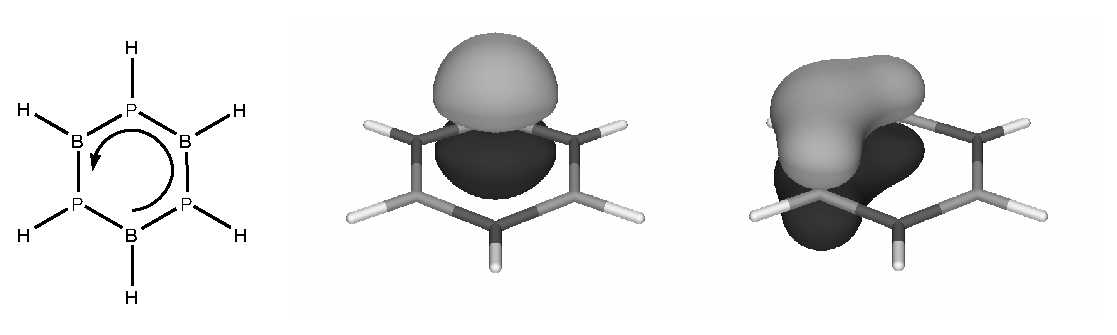
\includegraphics[width=5in]{introduction/figures/b3p3h6.eps}
\caption{Schematic ring current picture of B$_3$P$_3$H$_6$, together with an electron pair (two singly occupied orbitals), as calculated with VB.}
\label{ch1.fig.b3p3h6}
\end{figure}
 Although this molecule is not completely planar in its equilibrium (optimal) geometry, it is also still able to sustain a small induced diatropic ring current \cite{inorganic}.

In Chapter \chindacene\ the aromatic character of compounds fulfilling the 4$n$ $\pi$ electrons H\"{u}ckel rule for anti-aromaticity is examined. In molecules like $s$-indacene the central ring can be regarded as benzene, by drawing the two Kekul\'e-like structures in it. In that case, the two five membered rings will have an unpaired electron, which represents a bi-radical (Figure \ref{ch1.fig.indacene}). 
\begin{figure}[htp]
\center
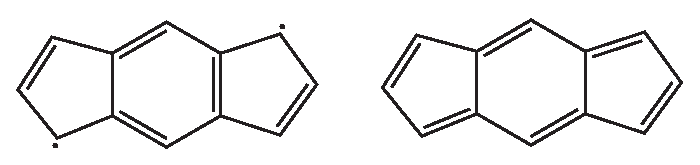
\includegraphics{introduction/figures/indacene.eps}
\caption{A structure with a Kekul\'e ring in the middle and two unpaired electrons (left) and a structure without bi-radical character of \textit{s}-indacene.}
\label{ch1.fig.indacene}
\end{figure}
In VB structures without bi-radical character, it is impossible to have Kekul\'e-like structures in the central ring, which has only two instead of three double bonds (Figure \ref{ch1.fig.indacene} (right)). By increasing the number of six membered rings, the aromatic character is expected to increase, resulting in more bi-radical character in the five membered rings. These effects are studied both with the Valence Bond method and \textit{ab initio} ring current density mapping \cite{indacene}.  

\bibliography{introduction}
\bibliographystyle{../main/achemso} 

\setcounter{chapter}{1}
\setcounter{NAT@ctr}{0}
\chapter{Orbital Optimization in Valence Bond Theory}
\label{chap_orbopt}

\ifthenelse{\boolean{wholethesis}}{\relax}{\begin{center}\textit{Generated on \today\ at \currenttime}\end{center}}

\noindent\textbf{Abstract:} The most time consuming step in optimizing a Valence Bond (VB) wave function is the construction of the matrix representation of the Hamilton operator ($\mathbf{H}$) and the corresponding overlap matrix ($\mathbf{S}$) for the wave function and the Brillouin states. In the 1990s a perturbation theory scheme, referred to as approximated Newton-Raphson (aNR), was introduced. For this scheme, not all $\mathbf{H}$ matrix elements need to be constructed. In this chapter an alternative, less time consuming method  to construct $\mathbf{H}$ matrix elements is introduced. In this method $\mathbf{H}$ matrix elements are replaced by elements of a Fock matrix.

\newpage

\section{Introduction}

\lettrine{\initial{I}}{}n 1916 Lewis suggested that atoms share electrons to form chemical bonds \cite{lewis}. Heitler and London incorporated this view a decade later into the quantum chemical description of the covalent bond in H$_2$ \cite{heitler}. In the 1930s Pauling used this description in his famous series of articles on ``The Nature Of The Chemical Bond'' \cite{pauling1,pauling2,pauling3,pauling4,pauling5,pauling6,pauling7,paulingbook}. This quantum chemical method is nowadays known as the Valence Bond theory.

In contrast to other methods, like the Molecular Orbital theory \cite{hartree1,hartree2,hartree3,fock} which use delocalized doubly occupied orbitals by default, the essential idea in Valence Bond theory is that atoms share electrons to form bonds. This is achieved by spin-pairing singly occupied orbitals on different atoms, or molecular fragments. The bond in H$_2$ can be described by the spin-coupling of the atomic $1s$ orbitals on both hydrogen atoms [H$\bullet$H$\bullet$]. The corresponding wave function consists of two determinants: $\Psi = |1s_{A}\overline{1s_{B}}| - |\overline{1s_{A}}1s_{B}|$. This determinant combination is called a structure. Since it describes the covalent character of the bond, it is referred to as the covalent structure. Ionic structures could be added to extend, or enhance the wave function: $|1s_{A}\overline{1s_{A}}|$ and $|1s_{B}\overline{1s_{B}}|$ (see Chapter \chintro). A VB wave function can be improved in two first. Firstly, more structures can be added. A disadvantage is that some structures may not have a clear chemical interpretation. Secondly, the wave function could be improved by optimization of the orbitals contained in the structures.

Besides the use of multiple determinants in VB, non-orthogonal and localized orbitals are used explicitly. Since the orbitals in MO theory can be chosen to be orthogonal, this method attracted more attention. Its implementation in computer programs is more straightforward and computations on larger molecular systems are possible. Despite its computational hurdles, progress in Valence Bond theory continued \cite{vboverv1,vboverv2,vboverv3}. One of the reasons is the chemical interpretation with the help of structures, not present in other methods. On the other hand several efficient methods to optimize Valence Bond wave functions, like Spin-Coupled Valence Bond (SCVB) \cite{scvb1,scvb2,scvb3} and Valence Bond Self-Consistent Field (VBSCF) \cite{vbscf1,vbscf2,koos1,zahid}, have been developed.

The most time consuming step in the optimization of the wave function is the optimization of the orbitals. Several optimization methods that compute the gradient of the total energy with respect to orbital rotations have been developed. The most common and widely applicable method is based on the evaluation of Hamiltonian matrix elements between Slater determinants, as introduced by L\"{o}wdin \cite{lowdin}. Despite it common applicability, this method is time consuming.

In another method, coined by Song \textit{et. al}, multiple Fock matrices are computed, one for each Slater determinant combination in the wave function \cite{song}. This approach is efficient and works fast for wave functions with a small number of Slater determinants. However, it is not as generally applicable as L\"{o}wdins method, because it can not be used for wave functions containing orthogonal orbitals that are variably occupied, \textit{i.e.} occur in some determinants, but not in all \cite{xmvb}. Although in VB non-orthogonal orbitals are used explicitly, orthogonality between the orbitals can occur.

In Multi Configurational Self-Consistent Field (MCSCF) \cite{joop,mcscf,roos1,roos2}, a method with similarities to VBSCF, elements of a common Fock matrix are used instead of Hamiltonian matrix elements computed via L\"{o}wdins formula \cite{roos1}. The central question for this chapter is whether it is also possible to use a single Fock matrix for the optimization of the orbitals in VBSCF, although those can be non-orthogonal. If multiple Hamiltonian matrix elements would be equal to elements from a single Fock matrix, it would not be necessary to construct these Hamiltonian matrix elements. This could save a considerable amount of computation time.

At first, the usability of Fock matrix elements instead of Hamiltonian matrix is analyzed by comparing the expression for Fock matrix elements with the expression for Hamiltonian matrix elements by L\"{o}wdin. Following this analysis, the implementation of these Fock matrix elements in TURTLE \cite{turtle}, the VB module in GAMESS-UK \cite{gamess}, will be presented. After the implementation details, speed-up factors of some test calculations will be discussed and compared. The chapter is concluded with an outlook on future enhancements.  

\section{Theory}

\subsection{\label{ch2.sec.vbsci}Valence Bond theory and Super CI}

To calculate the total energy of a molecular system, the time-independent Schr\"{o}dinger equation needs to be solved. The expectation value of the total energy for the system is:
\begin{equation}
E = \left< \Psi | \mathbf{H} | \Psi \right>,
\end{equation}
in which $\mathbf{H}$ is the Hamilton operator and $\Psi$ is the normalized wave function. A wave function is said to be optimized once the lowest possible value $E$ has been found. For Valence Bond theory, such a wave function $\Psi$ is constructed from a linear combination of structures:
\begin{equation}
\Psi = \sum_{i} C_i \Phi_i.
\label{ch2.eq.vbwf}
\end{equation}
These structures are linear combinations of Slater determinants:
\begin{equation}
\Phi = \sum_{i} \gamma_i \Delta_i,
\label{ch2.eq.struct}
\end{equation}
which are antisymmetrized products of spin-orbitals:
\begin{equation}
\Delta = |\chi_1\chi_2\chi_3\chi_4 \cdots \chi_n|,
\label{ch2.eq.determ}
\end{equation}
where the spin-orbitals $\chi$ have a spatial part ($\psi$) and a spin part which can be $\alpha$ or $\beta$. 
Orbitals $\psi$ are linear combinations of one electron basis functions:
\begin{equation}
\psi = \sum_{n} c_n \phi_n,
\label{ch2.eq.basis}
\end{equation}
in which the $c_n$ are orbital coefficients and $\phi_n$ one electron basis functions.

A Valence Bond wave function can be optimized by modifying the structure coefficients $C_i$ (equation \ref{ch2.eq.vbwf}) and the orbital coefficients $c_n$ (equation \ref{ch2.eq.basis}). Both optimizations can be performed simultaneously, as is done in a Newton-Raphson scheme \cite{zahid}, or sequentially with a method like Super CI \cite{superci1,superci2}. In Super CI, the structure coefficients $C_i$ are calculated first by solving the secular equation:
\begin{equation}
[\mathbf{H}-E\mathbf{S}] \cdot \mathbf{C} = 0,
\label{ch2.eq.eig}
\end{equation}
in which $\mathbf{H}$ and $\mathbf{S}$ are the Hamiltonian and overlap matrix in structure basis, respectively. Secondly, the orbitals are optimized, as will be explained below. After the orbital rotation the secular equation \ref{ch2.eq.eig} is solved again with the new orbitals until both sets of coefficients no longer change.

The $\mathbf{H}$-matrix elements in equation \ref{ch2.eq.eig} are computed with L\"{o}wdins formula for each determinant combination in $\Psi$:
\begin{equation}
\begin{split}
\left< \Psi | \mathbf{H} | \Psi \right> &= \sum_{pq} C_p C_q \left< \Delta_p | \mathbf{H} | \Delta_q \right> \\ 
&= \sum_{pq} C_p C_q \left(\sum_{ik} h_{ik} \cdot S^{(i,k)} + \sum_{i<j,k<l} \left\{ \left[ \chi_i \chi_k | \chi_j \chi_l \right] - \left[ \chi_i \chi_l | \chi_j \chi_k \right] \right\} \cdot S^{(i,j,k,l)}\right),
\end{split}
\label{ch2.eq.lowdindeterminants}
\end{equation}
where $C_p$ and $C_q$ are determinant coefficients, $\Delta_p$ and $\Delta_q$ are determinants, $S^{(i,k)}$ and $S^{(i,j,k,l)}$ are first and second order cofactors\footnote{Cofactors are described in detail in Appendix A.}  and $h_{ik}$ and the term between curly brackets are one and two electron integrals, respectively.

Orbitals can be changed by adding a small amount of an other orbital. For instance, orbital $\psi_i$ can be changed by adding a small amount $\delta b_{ia}$ times $\psi_a$:
\begin{equation}
\psi_i' = \psi_i + \delta b_{ia} \psi_a.
\label{ch2.eq.orbchange}
\end{equation}
As a simple example, a single determinant wave function $\Psi_0=|\psi_i\overline{\psi_i}\psi_j\psi_k|$ with four orbitals is chosen. The orbital change of equation \ref{ch2.eq.orbchange} will result in:
\begin{equation}    
\begin{split}
|\psi_i'\overline{\psi_i'}\psi_j\psi_k | & = |(\psi_i + \delta b_{ia} \psi_a)\overline{(\psi_i + \delta b_{ia}\psi_a)}\psi_j\psi_k |\\
& = |\psi_i\overline{\psi_i}\psi_j\psi_k| + \delta b_{ia}|\psi_a\overline{\psi_i}\psi_j\psi_k| + \delta b_{ia} |\psi_i\overline{\psi_a}\psi_j\psi_k| + \delta b^2_{ia} |\psi_a\overline{\psi_a}\psi_j\psi_k|.\\
\end{split}
\label{ch2.eq.detchange}
\end{equation}
The first term is the original wave function $\Psi_0$. The second and third term are determinants, in which orbital $\psi_i$ has been replaced by $\psi_a$, once for $\alpha$ and once for $\beta$ spin. In the fourth determinant both occurrences of orbital $\psi_i$ have been replaced by $\psi_a$. This fourth determinant will be neglected here, because the amount $\delta b_{ia}$ is considered small and hence $\delta b_{ia}^2 \approx 0$.

The combination of the second and third determinant can be created from $|\psi_i\overline{\psi_i}\psi_j\psi_k |$ by the single excitation operator $\mathbf{C}_{i \rightarrow a}$, which replaces $\psi_i$ by $\psi_a$, once for $\alpha$ spin and once for $\beta$ spin \cite{ruttink}. This singly excited structure will be referred to as $\Psi_{ia}$. The change in $\Psi_0$ caused by the orbital change results (to first order) in:
\begin{equation}
\Psi_{0} \rightarrow \Psi_{0} + \delta b_{ia} \mathbf{C}_{i \rightarrow a} \Psi_{0} = \Psi_{0} + \delta b_{ia} \Psi_{ia}.
\label{ch2.eq.wfchange}
\end{equation}

With this mechanism orbital $\psi_i$ could be changed in such a way that the expectation value of the energy of $\Psi_0$ becomes lower. The minimum in the energy is found when the first order derivative of the energy with respect to the orbital change equals zero:
\begin{equation}
\frac{\partial E}{\partial b_{ia}}=\frac{\partial \frac{\left < \Psi_0 | \mathbf{H} | \Psi_0 \right >}{\left < \Psi_0 | \Psi_0 \right >}}{\partial b_{ia}}=0.
\label{ch2.eq.foderiv}
\end{equation}
Using the quotient rule, using the fact that $\left < \Psi_0 | \mathbf{H} | \Psi_0 \right >$ and $\left < \Psi_0 | \Psi_0 \right >$ are symmetric and using that the first order derivative with respect to the orbital change of $\Psi_0$ in equation \ref{ch2.eq.wfchange} equals $\Psi_{ia}$ \cite{vbscf2}, the first order derivative of the energy with respect to the orbital change can be written as: 
\begin{equation}
\begin{split}
\frac{\partial E}{\partial b_{ia}} & = \frac{2 \cdot \left < \Psi_0 | \mathbf{H} | \Psi_{ia} \right > \left< \Psi_0 | \Psi_0 \right > - 2 \cdot \left < \Psi_0 | \mathbf{H} | \Psi_0  \right > \left< \Psi_0 | \Psi_{ia}\right>}{\left < \Psi_0 | \Psi_0 \right > ^2 }\\
& = \frac{ 2 \cdot \left < \Psi_0 | \mathbf{H} | \Psi_{ia} \right > - 2 \cdot E_0 \left< \Psi_0 | \Psi_{ia} \right >}{\left < \Psi_0 | \Psi_0 \right >}\\
& = \frac{ 2 \cdot \left < \Psi_0 | \mathbf{H} - E_0 | \Psi_{ia} \right >}{\left < \Psi_0 | \Psi_0 \right >}.
\end{split}
\label{ch2.eq.foderiv2}
\end{equation}
For optimal orbitals, this first order derivative is equal to zero and hence:
\begin{equation}
\left < \Psi_0 | \mathbf{H} - E_0 | \Psi_{ia} \right > = 0.
\label{ch2.eq.brillouin}
\end{equation}
This is the Brillouin theorem, which states that with optimal orbitals singly excited states ($\Psi_{ia}$) do not interact or mix with the reference or ground state ($\Psi_0$) \cite{brillouin,genbrill}. 

In equations \ref{ch2.eq.orbchange}-\ref{ch2.eq.brillouin} the effect of a single orbital change has been shown. When all possible single excitations are taken into account, the wave function of equation \ref{ch2.eq.wfchange} can be written as:
\begin{equation}
\Psi_{superci} = \Psi_0 + \sum_{ia} b_{ia} \Psi_{ia},
\label{ch2.eq.superci}
\end{equation}
in which $\Psi_{superci}$ is the Super CI wave function, $i$ runs over all orbitals from which an excitation can be performed and $a$ runs over all orbitals to which excitations can take place. Values for $b_{ia}$ can be found by solving the generalized eigenvalue problem:
\begin{equation}
[\mathbf{H}-E_b\mathbf{S}] \cdot \mathbf{b} = 0,
\label{ch2.eq.geig}
\end{equation}
in which $\mathbf{H}$ and $\mathbf{S}$ are the Hamiltonian and metric in the basis of $\Psi_0$ and the singly excited states. $E_b$ is the lowest eigenvalue and $\mathbf{b}$ is the corresponding eigenvector. With the elements of $\mathbf{b}$ the orbitals are updated to make $\Psi_0$ equal to $\Psi_{superci}$ to first order:
\begin{equation}
\psi_i' = \psi_i + \sum_{a} b_{ia} \psi_a.
\label{ch2.eq.orbupd}
\end{equation}
With the modification of the orbitals the Super CI wave function is contracted or condensed into $\Psi_0$. This is exemplified for the change in orbital $\psi_i$ in the simple one determinant wave function in equation \ref{ch2.eq.detchange}. Orbital $\psi_i$ in $\Psi_0$ is modified with $\delta b_{ia}$ times orbital $\psi_a$, which results in determinant $|\psi_i'\overline{\psi_i'}\psi_j\psi_k |$:
\begin{equation}
\begin{split}
\Psi_{0} \leftarrow & \Psi_{0} + \delta b_{ia} \Psi_{ia} = \\
&|\psi_i\overline{\psi_i}\psi_j\psi_k| + \delta b_{ia}(|\psi_a\overline{\psi_i}\psi_j\psi_k| + |\psi_i\overline{\psi_a}\psi_j\psi_k|) \approx \\
&|(\psi_i + \delta b_{ia}\psi_a)\overline{(\psi_i + \delta b_{ia}\psi_a)}\psi_j\psi_k| = \\
&|\psi_i'\overline{\psi_i'}\psi_j\psi_k |.\\
\end{split}
\label{ch2.eq.condense}
\end{equation}
So, $\Psi_0$ will contain the updated orbital $\psi_i'$ which will be denoted $\psi_i$ in the next step (iteration). This procedure for a single orbital update is performed for all combinations in the summation in the Super CI wave function. Since the orbital changes are performed independently, they may be counteracting and therefore the Brillouin condition may not be fulfilled in a single step. Therefore, a new excitation pattern for a new $\Psi_{superci}$ is created. The eigenvalue problem is solved again and the orbitals are updated once more. It is expected that the orbital updates become smaller with each step. This procedure is repeated until all Brillouin elements, $\left < \Psi_0 | \mathbf{H} - E_0 | \Psi_{ia} \right >$, have become zero. At that point the expectation value of the energy ($E_0$) is stationary with respect to orbital changes (equation \ref{ch2.eq.foderiv2}).

Up till here, $\Psi_0$ was constructed of a single determinant, \textit{i.e.} $|\psi_i\overline{\psi_i}\psi_j\psi_k|$. A regular VB wave function consists of multiple structures, and hence multiple determinants (see equations \ref{ch2.eq.vbwf} and \ref{ch2.eq.struct}). In that case, the contraction of equation \ref{ch2.eq.condense} will contain more determinants, all in which orbital $\psi_i$ has been replaced by $\psi_a$.

To solve the generalized eigenvalue problem of equation \ref{ch2.eq.geig}, both the Hamiltonian ($\mathbf{H}$) and the overlap ($\mathbf{S}$) are expressed in matrix form.  The Brillouin matrix is defined as the $\mathbf{H}$ matrix minus $E_0$ \cite{koos1}. Please note that for optimal orbitals, the Brillouin energy ($E_b$) in equation \ref{ch2.eq.geig} is equal to the energy of the ground state ($E_0$), because the singly exited states do no longer mix in with the ground state. 

An example of a Brillouin matrix, which contains elements resulting from two excitations: an excitation from $\psi_i$ to $\psi_a$ ($\Psi_{ia}$) and one from $\psi_i$ to $\psi_b$ ($\Psi_{ib}$), is shown below:
\begin{equation}
\left[\begin{array}{ccc}
\left< \Psi_{0} | \mathbf{H}-E_0 | \Psi_{0} \right> & \left< \Psi_{ia} | \mathbf{H}-E_0 | \Psi_{0} \right> & \left< \Psi_{ib} | \mathbf{H}-E_0 | \Psi_{0} \right> \\
\left< \Psi_{0} | \mathbf{H}-E_0 | \Psi_{ia} \right> & \left< \Psi_{ia} | \mathbf{H}-E_0 | \Psi_{ia} \right> & \left< \Psi_{ib} | \mathbf{H}-E_0 | \Psi_{ia} \right> \\
\left< \Psi_{0} | \mathbf{H}-E_0 | \Psi_{ib} \right> & \left< \Psi_{ia} | \mathbf{H}-E_0 | \Psi_{ib} \right> & \left< \Psi_{ib} | \mathbf{H}-E_0 | \Psi_{ib} \right> \\
\end{array}\right].
\label{ch2.eq.hamilt}
\end{equation}
The Brillouin matrix has the same dimension as the $\mathbf{H}$ and $\mathbf{S}$ matrices in equation \ref{ch2.eq.geig}. The calculation of the elements in $\mathbf{H}$ is expensive because of the large number of determinants, caused by the expansion into the Super CI wave function: for each excitation a Brillouin state, containing 1 to 2 times the number of determinants of $\Psi_0$, is added. For each determinant combination the evaluation of (large amounts of) subdeterminants \cite{koos2}, or cofactors are required.

To lower the computation time, Van Lenthe \textit{et al.} introduced a method, referred to as approximated Newton-Raphson (Section \ref{ch2.sec.anr}) \cite{koos1}, which requires less $\mathbf{H}$ and $\mathbf{S}$ matrix elements than regular Super CI \cite{koos1}, because elements of the type $\left < \Psi_{ia} | \mathbf{H} - E_0 | \Psi_{ib} \right >$ are not needed. This method will be explained in the next section.

\subsection{\label{ch2.sec.anr}The Approximated Newton-Raphson Method}

In the approximated Newton-Raphson technique perturbation theory is used to obtain orbital update coefficients. These coefficients are approximated by the quotient of the first column element and the diagonal element on each row of equation \ref{ch2.eq.hamilt}:
\begin{equation}
b_{ia}= - \frac{\left< \Psi_{0} | \mathbf{H}-E_0 | \Psi_{ia} \right>}{\left< \Psi_{ia} | \mathbf{H}-E_0 | \Psi_{ia} \right>}.
\label{ch2.eq.anr}
\end{equation}
This means that elements of the type $\left< \Psi_{ia} | \mathbf{H}-E_0 | \Psi_{ib} \right>$ are not used. In that way, only two matrix elements need to be calculated for such an excitation, instead of $m$, where $m$ equals the total number of excitations. This reduces the quadratic increase in number of matrix elements to linear.

Although the update coefficients $b_{ia}$ are calculated in a different way, the total energy $E_0$ will be the same. Once the orbitals are optimal the numerator in equation \ref{ch2.eq.anr} becomes zero and hence the Brillouin condition is fulfilled. 

A further reduction of the calculation time can be achieved if the numerator and the denominator in equation \ref{ch2.eq.anr} could be calculated, or approximated, faster. The Fock matrix elements depend on the number of determinants in the reference wave function, while the Brillouin matrix elements in equation \ref{ch2.eq.anr} depend on the determinants in the expanded Super CI wave function. Furthermore, multiple Brillouin matrix elements can be replaced by elements of a single Fock matrix. In the next section, the applicability of Fock matrix elements for the numerator and denominator in equation \ref{ch2.eq.anr} will be investigated.

\subsection{\label{ch2.sec.fock}Fock Matrix Elements} 

Roos \textit{et al.} showed that Brillouin matrix elements of the type $\left< \Psi_0 | \mathbf{H} | \Psi_{ia} \right>$ (the numerator in equation \ref{ch2.eq.anr}) could be replaced by elements of the Fock matrix ($F_{ia}$) for Complete Active Space Self-Consistent Field (CASSCF) wave functions \cite{roos1}. A CASSCF wave function is an MCSCF wave function for which all possible electron distributions in the variably occupied orbital space are included. The Fock matrix elements have the form:
\begin{equation}
F_{ia} = h_{ia} + \sum_{\sigma\nu} \left\{ \left[ \chi_i \chi_a | \chi_\sigma \chi_\nu \right] - \left[ \chi_i \chi_\nu | \chi_\sigma \chi_a \right] \right\} \cdot P^{(\sigma,\nu)},
\label{ch2.eq.fock}
\end{equation}
in which $F_{ia}$ is the Fock matrix element of spin-orbitals $\chi_i$ and $\chi_a$, $h_{ia}$ is the one electron integral $\left< \chi_i | \mathbf{h}| \chi_a \right>$. The double sum (over $\sigma$ and $\nu$) on the right hand side is over two electron integrals (Coulomb and exchange) times elements of the density matrix $P^{(\sigma,\nu)}$. Indices $\sigma$ and $\nu$ run over all occupied orbitals. Therefore, the dimension of the density matrix is the number of occupied orbitals ($\sigma$) by the number of occupied orbitals ($\nu$). Density matrix elements are constructed from first order cofactors, taken from $\left< \Psi_0 | \Psi_0 \right>$. Examples are given in equations \ref{ch2.eq.p0exampg}, \ref{ch2.eq.p0examp} and \ref{ch2.eq.p0examp2}.

In multideterminant wave functions, three orbital classes can be distinguished. The first class contains those orbitals that occur in all determinants. These will be denoted with labels $i$, $j$, $k$ and $l$. The second class contains orbitals that occur in some determinants, denoted with $t$, $u$, $v$ and $x$. The last class contains those orbitals that do not occur in the ground state wave function $\Psi_0$ and hence are virtual unoccupied orbitals, labeled $a$, $b$, $c$ and $d$. With those classes in mind, Roos \textit{et al.} published three expressions with Fock matrix elements for three types of excitations:
\begin{itemize}
\item{$i \rightarrow a$ from (always) doubly occupied to virtual orbitals}
\item{$t \rightarrow a$ from variably occupied to virtual orbitals}
\item{$i \rightarrow t$ from (always) doubly to variably occupied orbitals}
\end{itemize}
The fourth type of excitation, $t \rightarrow t$ from variably to variably occupied orbitals, is not needed in CASSCF, because all possible electron distributions in the variably occupied orbital space are already included in $\Psi_0$. In this section the applicability of Fock matrix elements in the construction of Brillouin matrix elements in VBSCF will be analyzed with L\"{o}wdins formula, equation \ref{ch2.eq.lowdindeterminants}. The difference between the one electron parts of L\"{o}wdins formula (equation \ref{ch2.eq.lowdindeterminants}) and the expression for a Fock matrix element (equation \ref{ch2.eq.fock}) is that in the former multiple one electron integrals are multiplied by first order cofactors ($S^{(i,k)}$), while in the later only a single one electron integral occurs without a multiplication factor. Furthermore, the two electron integral part in the former is multiplied by second order cofactors ($S^{(i,j,k,l)}$), while in the latter those are multiplied by elements of the density matrix ($P^{(\sigma,\nu)}$). To analyze in which situations Fock matrix elements are equal to Brillouin matrix elements, a comparison of the cofactors in equation \ref{ch2.eq.lowdindeterminants} and the density matrix elements in equation \ref{ch2.eq.fock} is needed.

For this comparison the single determinant wave function $\Psi_0 = |\chi_1\chi_2\chi_3\chi_4\chi_5|$ is chosen. The excitation that will be examined for this wave function is from $\chi_1$ to $\chi_6$. Hence, $\Psi_{16}$ is equal to $|\chi_6\chi_2\chi_3\chi_4\chi_5|$. Numerals have been chosen as subscripts, rather than the previously specified letters: the classification of orbitals should not blur this comparison. 

The orbitals $\chi$ are normalized, \textit{i.e.} $\left< \chi_1 | \chi_1 \right> = 1$. Throughout this chapter, normalized wave functions are used. This means that the determinants are multiplied by normalization constants in such a way that $\left< \Psi_0 |  \Psi_0 \right> = 1$:
\begin{equation}
\left < \Psi_0 | \Psi_0 \right> = | \mathbf{S} | = \frac{1}{N} \cdot
\begin{array}{llllll}
 &  \chi_1 & \chi_2 & \chi_3 & \chi_4 & \chi_5 \\
 \chi_1 & \multicolumn{1}{|l}{ 1 } & s_{21} & s_{31} & s_{41} & \multicolumn{1}{l|}{ s_{51} } \\
 \chi_2 & \multicolumn{1}{|l}{ s_{12} } & 1 & s_{32} & s_{42} & \multicolumn{1}{l|}{ s_{52} } \\
 \chi_3 & \multicolumn{1}{|l}{ s_{13} } & s_{23} & 1 & s_{43} & \multicolumn{1}{l|}{ s_{53} } \\
 \chi_4 & \multicolumn{1}{|l}{ s_{14} } & s_{24} & s_{34} & 1 & \multicolumn{1}{l|}{ s_{54} } \\
 \chi_5 & \multicolumn{1}{|l}{ s_{15} } & s_{25} & s_{35} & s_{45} & \multicolumn{1}{l|}{ 1 }
\end{array} = 1,
\label{ch2.eq.s0g}
\end{equation}
in which the $s$ elements are overlaps between orbitals and $\frac{1}{N}$ is the normalization constant\footnote{Throughout this chapter normalized wave functions are used. Therefore, the normalization constant $\frac{1}{N}$ is implicitly included.}. For example, $s_{34} = \left< \chi_3 | \chi_4 \right>$. The density matrix, needed for the Fock matrix, is constructed from subdeterminants of this determinant. An example of a density matrix element is $P^{(3,4)}$:
\begin{equation}
P^{(3,4)}=
\begin{array}{llllll}
 & \hskip 53.0 pt \hbox{\lower 93pt\hbox{\vrule height100pt width 1.0pt}}\hskip-54.0pt \chi_1 & \chi_2 & \chi_3 & \chi_4 & \chi_5 \\
 \noalign{\vskip-91pt}
 \chi_1 & \multicolumn{1}{|l}{ 1 } & s_{21} & s_{31} & s_{41} & \multicolumn{1}{l|}{ s_{51} } \\
 \chi_2 & \multicolumn{1}{|l}{ s_{12} } & 1 & s_{32} & s_{42} & \multicolumn{1}{l|}{ s_{52} } \\
 \chi_3 & \multicolumn{1}{|l}{ s_{13} } & s_{23} & 1 & s_{43} & \multicolumn{1}{l|}{ s_{53} } \\
 \chi_4 & \multicolumn{1}{|l}{ s_{14} } & s_{24} & s_{34} & 1 & \multicolumn{1}{l|}{ s_{54} } \\
 \noalign{\vskip-8pt}
 \multispan6\hbox{\vrule  height 1.0 pt width140pt}\cr
 \noalign{\vskip 7pt}
 \chi_5 & \multicolumn{1}{|l}{ s_{15} } & s_{25} & s_{35} & s_{45} & \multicolumn{1}{l|}{ 1 }
\end{array} =
\begin{array}{lllll}
 &  \chi_1 & \chi_2 & \chi_4 & \chi_5 \\
 \chi_1 & \multicolumn{1}{|l}{ 1 } & s_{21} & s_{41} & \multicolumn{1}{l|}{ s_{51} } \\
 \chi_2 & \multicolumn{1}{|l}{ s_{12} } & 1 & s_{42} & \multicolumn{1}{l|}{ s_{52} } \\
 \chi_3 & \multicolumn{1}{|l}{ s_{13} } & s_{23} & s_{43} & \multicolumn{1}{l|}{s_{53}} \\
 \chi_5 & \multicolumn{1}{|l}{ s_{15} } & s_{25} & s_{45} & \multicolumn{1}{l|}{1}
\end{array},
\label{ch2.eq.p0exampg}
\end{equation}
which is the subdeterminant of $|\mathbf{S}|$ (equation \ref{ch2.eq.s0g}), from which the third column and the fourth row are removed.

First and second order cofactors that occur in equation \ref{ch2.eq.lowdindeterminants} are subdeterminants of the overlap determinant of $\Psi_0$ with $\Psi_{16}$:
\begin{equation}
\left < \Psi_0 | \Psi_{16} \right> =
\begin{array}{llllll}
 &  \chi_1 & \chi_2 & \chi_3 & \chi_4 & \chi_5 \\
 \chi_6 & \multicolumn{1}{|l}{ s_{16} } & s_{26} & s_{36} & s_{46} & \multicolumn{1}{l|}{ s_{56} } \\
 \chi_2 & \multicolumn{1}{|l}{ s_{12} } & 1 & s_{32} & s_{42} & \multicolumn{1}{l|}{ s_{52} } \\
 \chi_3 & \multicolumn{1}{|l}{ s_{13} } & s_{23} & 1 & s_{43} & \multicolumn{1}{l|}{ s_{53} } \\
 \chi_4 & \multicolumn{1}{|l}{ s_{14} } & s_{24} & s_{34} & 1 & \multicolumn{1}{l|}{ s_{54} } \\
 \chi_5 & \multicolumn{1}{|l}{ s_{15} } & s_{25} & s_{35} & s_{45} & \multicolumn{1}{l|}{ 1 }
\end{array}.
\label{ch2.eq.s016g}
\end{equation}
An example of a first order cofactor from $\left < \Psi_0 | \Psi_{16} \right>$ is $S^{(3,4)}$:
\begin{equation}
S^{(3,4)}=
\begin{array}{llllll}
 & \hskip 53.0 pt \hbox{\lower 93pt\hbox{\vrule height100pt width 1.0pt}}\hskip-54.0pt \chi_1 & \chi_2 & \chi_3 & \chi_4 & \chi_5 \\
 \noalign{\vskip-91pt}
 \chi_6 & \multicolumn{1}{|l}{ s_{16} } & s_{26} & s_{36} & s_{46} & \multicolumn{1}{l|}{ s_{56} } \\
 \chi_2 & \multicolumn{1}{|l}{ s_{12} } & 1 & s_{32} & s_{42} & \multicolumn{1}{l|}{ s_{52} } \\
 \chi_3 & \multicolumn{1}{|l}{ s_{13} } & s_{23} & 1 & s_{43} & \multicolumn{1}{l|}{ s_{53} } \\
 \chi_4 & \multicolumn{1}{|l}{ s_{14} } & s_{24} & s_{34} & 1 & \multicolumn{1}{l|}{ s_{54} } \\
 \noalign{\vskip-8pt}
 \multispan6\hbox{\vrule  height 1.0 pt width140pt}\cr
 \noalign{\vskip 7pt}
 \chi_5 & \multicolumn{1}{|l}{ s_{15} } & s_{25} & s_{35} & s_{45} & \multicolumn{1}{l|}{ 1 }
\end{array} =
\begin{array}{lllll}
 &  \chi_1 & \chi_2 & \chi_4 & \chi_5 \\
 \chi_6 & \multicolumn{1}{|l}{ s_{16} } & s_{26} & s_{46} & \multicolumn{1}{l|}{ s_{56} } \\
 \chi_2 & \multicolumn{1}{|l}{ s_{12} } & 1 & s_{42} & \multicolumn{1}{l|}{ s_{52} } \\
 \chi_3 & \multicolumn{1}{|l}{ s_{13} } & s_{23} & s_{43} & \multicolumn{1}{l|}{s_{53}} \\
 \chi_5 & \multicolumn{1}{|l}{ s_{15} } & s_{25} & s_{45} & \multicolumn{1}{l|}{1}
\end{array}.
\label{ch2.eq.s16g}
\end{equation}

On the first row in both determinants of equation \ref{ch2.eq.s16g} there are orbital overlaps, like $s_{26}$, which do not occur in the overlap determinant $\left< \Psi_0 | \Psi_0 \right>$. However, there are 5 out of 25 first order cofactors which have a corresponding $P$-matrix element, \textit{i.e} the cofactors $S^{(n,6)}$ are equal to $P^{(n,1)}$, for $n$ in \{1,2,3,4,5\}. In general, $m$ out of $m^2$ first order cofactors have a corresponding value in the $P$-matrix, where $m$ is the number of electrons. Hence, without any orthogonality present in the wave function and/or its singly excited states, the usability of the Fock matrix built from the density matrix is only useful for $\frac{m}{m^2}$ elements of the Brillouin matrix. 

In TURTLE, the virtual orbitals are chosen orthogonal to all other orbitals (see the Appendix of reference \cite{koos1}). If $\chi_6$ would be such a virtual orbital, the overlap of $\Psi_0$ with $\Psi_{16}$ becomes:
\begin{equation}
\left < \Psi_0 | \Psi_{16} \right> =
\begin{array}{llllll}
 &  \chi_1 & \chi_2 & \chi_3 & \chi_4 & \chi_5 \\
 \chi_6 & \multicolumn{1}{|l}{ 0 } & 0 & 0 & 0 & \multicolumn{1}{l|}{ 0 } \\
 \chi_2 & \multicolumn{1}{|l}{ s_{12} } & 1 & s_{32} & s_{42} & \multicolumn{1}{l|}{ s_{52} } \\
 \chi_3 & \multicolumn{1}{|l}{ s_{13} } & s_{23} & 1 & s_{43} & \multicolumn{1}{l|}{ s_{53} } \\
 \chi_4 & \multicolumn{1}{|l}{ s_{14} } & s_{24} & s_{34} & 1 & \multicolumn{1}{l|}{ s_{54} } \\
 \chi_5 & \multicolumn{1}{|l}{ s_{15} } & s_{25} & s_{35} & s_{45} & \multicolumn{1}{l|}{ 1 }
\end{array}.
\label{ch2.eq.s016go}
\end{equation}
In that case, there are only 5 first order cofactors, $S^{(n,6)}$ ($n$ in \{1,2,3,4,5\}), because the other first order cofactors are zero: there will be zeroes on the first row, making these determinants zero. As seen before, these 5 cofactors all have a corresponding $P$-matrix element, $P^{(n,1)}$. Whether it is possible to use these to construct Fock matrix elements for use in Brillouin matrix elements will be investigated for the excitation types $i \rightarrow a$ and $t \rightarrow a$. In those excitations, an orthogonal virtual is used.

Brillouin matrix elements of the type $i \rightarrow t$ and $t \rightarrow t$ have first order cofactors like in equation \ref{ch2.eq.s016g}. Because these contain overlaps that do not occur in $\left< \Psi_0 | \Psi_0 \right>$, they are not equal to density matrix elements. This means that Fock matrix elements could only be used for $m$ out of $m^2$ Brillouin matrix elements. In every day Valence Bond wave functions, multiple orbitals occur and so $m^2$ will be much larger than $m$. Therefore, Brillouin matrix elements of the type $i \rightarrow t$ and $t \rightarrow t$ will be constructed the usual way via L\"{o}wdins formula (equation \ref{ch2.eq.lowdindeterminants}).

\subsubsection{\label{ch2.sec.i-a}$i \rightarrow a$ from (always) doubly occupied to virtual orbitals}

To investigate the excitation type $i \rightarrow a$, the 5 electron wave function $|\chi_1\chi_2\chi_3\chi_4\chi_5|$ is changed into $|\chi_i\chi_j\chi_t\chi_u\chi_v|$, in which $\chi_i$ is $\psi_i$, $\chi_j$ is $\overline{\psi_i}$ and $\chi_t$, $\chi_u$ and $\chi_v$ are singly occupied orbitals. Spin for these orbitals is not specified and hence no attention needs to be paid to the spin integration in the overlap matrices that follow. Doubly occupied orbitals occur in all determinants and can be chosen orthogonal to all other orbitals \cite{koos1}. Although the 5 spin orbitals occur in ``all'' determinants in this single determinant wave function, $\chi_i$ and $\chi_j$ are chosen orthogonal to all other orbitals, while $\chi_t$, $\chi_u$ and $\chi_v$ are non-orthogonal to each other. Later on, the derivation for this single determinant wave function will be expanded for a multideterminant wave function in which orbitals $\chi_t$, $\chi_u$ and $\chi_v$ are variably occupied. The norm $\left < \Psi_0 | \Psi_0 \right>$ is the determinant of the overlap matrix, which will then have the following layout:
\begin{equation}
\left < \Psi_0 | \Psi_0 \right> = | \mathbf{S} | =
\begin{array}{llllll}
 &  \chi_i & \chi_j & \chi_t & \chi_u & \chi_v \\
 \chi_i & \multicolumn{1}{|l}{ 1 } & 0 & 0 & 0 & \multicolumn{1}{l|}{ 0 } \\
 \chi_j & \multicolumn{1}{|l}{ 0 } & 1 & 0 & 0 & \multicolumn{1}{l|}{ 0 } \\
 \chi_t & \multicolumn{1}{|l}{ 0 } & 0 & 1 & s_{ut} & \multicolumn{1}{l|}{s_{vt}} \\
 \chi_u & \multicolumn{1}{|l}{ 0 } & 0 & s_{tu} & 1 & \multicolumn{1}{l|}{s_{vu}} \\
 \chi_v & \multicolumn{1}{|l}{ 0 } & 0 & s_{tv} & s_{uv} & \multicolumn{1}{l|}{1}
\end{array}.
\label{ch2.eq.s0}
\end{equation}

In analogy with the example density matrix element in equation \ref{ch2.eq.p0exampg}, an example from density matrix element $P^{(t,u)}$, a cofactor of the norm in equation \ref{ch2.eq.s0}, is:
\begin{equation}
P^{(t,u)}=
\begin{array}{llllll}
 & \hskip 46.0 pt \hbox{\lower 93pt\hbox{\vrule height100pt width 1.0pt}}\hskip-47.0pt \chi_i & \chi_j & \chi_t & \chi_u & \chi_v \\
 \noalign{\vskip-91pt}
 \chi_i &  \multicolumn{1}{|l}{ 1 } & 0 & 0 & 0 & \multicolumn{1}{l|}{ 0 } \\
 \chi_j & \multicolumn{1}{|l}{ 0 } & 1 & 0 & 0 & \multicolumn{1}{l|}{ 0 } \\
 \chi_t & \multicolumn{1}{|l}{ 0 } & 0 & 1 & s_{ut} & \multicolumn{1}{l|}{s_{vt}} \\
 \chi_u & \multicolumn{1}{|l}{ 0 } & 0 & s_{tu} & 1 & \multicolumn{1}{l|}{s_{vu}} \\
 \noalign{\vskip-8pt}
 \multispan6\hbox{\vrule  height 1.0 pt width130pt}\cr
 \noalign{\vskip 7pt}
 \chi_v & \multicolumn{1}{|l}{ 0 } & 0 & s_{tv} & s_{uv} & \multicolumn{1}{l|}{ 1 }
\end{array} =
\begin{array}{lllll}
 &  \chi_i & \chi_j & \chi_u & \chi_v \\
 \chi_i & \multicolumn{1}{|l}{ 1 } & 0 & 0 & \multicolumn{1}{l|}{ 0 } \\
 \chi_j & \multicolumn{1}{|l}{ 0 } & 1 & 0 & \multicolumn{1}{l|}{ 0 } \\
 \chi_t & \multicolumn{1}{|l}{ 0 } & 0 & s_{ut} & \multicolumn{1}{l|}{s_{vt}} \\
 \chi_v & \multicolumn{1}{|l}{ 0 } & 0 & s_{uv} & \multicolumn{1}{l|}{1}
\end{array}.
\label{ch2.eq.p0examp}
\end{equation}

Since $\psi_i$ is doubly occupied, in $\chi_i$ and $\chi_j$, there are also two virtual orbitals for $\psi_a$, being $\chi_a \equiv \psi_a$ and $\chi_b \equiv \overline{\psi_a}$. The singly excited state wave function is $\Psi_{ia} = |\chi_a\chi_j\chi_t\chi_u\chi_v| + |\chi_i\chi_b\chi_t\chi_u\chi_v|$. These determinants will be referred to as $\Delta_{ia}$ and $\Delta_{jb}$, respectively. The overlap between $\Psi_0$, denoted here as $\Delta_0$, and both these determinants is:
\begin{equation}
\left < \Delta_0 | \Delta_{ia} \right > = 
\begin{array}{llllll}
 &  \chi_i & \chi_j & \chi_t & \chi_u & \chi_v \\
 \chi_a & \multicolumn{1}{|l}{ 0 } & 0 & 0 & 0 & \multicolumn{1}{l|}{ 0 } \\
 \chi_j & \multicolumn{1}{|l}{ 0 } & 1 & 0 & 0 & \multicolumn{1}{l|}{ 0 } \\
 \chi_t & \multicolumn{1}{|l}{ 0 } & 0 & 1 & s_{ut} & \multicolumn{1}{l|}{s_{vt}} \\
 \chi_u & \multicolumn{1}{|l}{ 0 } & 0 & s_{tu} & 1 & \multicolumn{1}{l|}{s_{vu}} \\
 \chi_v & \multicolumn{1}{|l}{ 0 } & 0 & s_{tv} & s_{uv} & \multicolumn{1}{l|}{1}
\end{array}
\label{ch2.eq.psi0_ia}
\end{equation}
and
\begin{equation}
\left < \Delta_0 | \Delta_{jb} \right > = 
\begin{array}{llllll}
 &  \chi_i & \chi_j & \chi_t & \chi_u & \chi_v \\
 \chi_i & \multicolumn{1}{|l}{ 1 } & 0 & 0 & 0 & \multicolumn{1}{l|}{ 0 } \\
 \chi_b & \multicolumn{1}{|l}{ 0 } & 0 & 0 & 0 & \multicolumn{1}{l|}{ 0 } \\
 \chi_t & \multicolumn{1}{|l}{ 0 } & 0 & 1 & s_{ut} & \multicolumn{1}{l|}{s_{vt}} \\
 \chi_u & \multicolumn{1}{|l}{ 0 } & 0 & s_{tu} & 1 & \multicolumn{1}{l|}{s_{vu}} \\
 \chi_v & \multicolumn{1}{|l}{ 0 } & 0 & s_{tv} & s_{uv} & \multicolumn{1}{l|}{1}
\end{array},
\label{ch2.eq.psi0_jb}
\end{equation}
which are both zero, because they contain a row and a column with zeroes.

To construct the Brillouin matrix element (equation \ref{ch2.eq.lowdindeterminants}), first and second order cofactors from the determinants in equations \ref{ch2.eq.psi0_ia} and \ref{ch2.eq.psi0_jb} are needed. Only two first order cofactors have a nonzero value, $S^{(i,a)}$ created by removing column $\chi_i$ and row $\chi_a$ from the determinant in equation \ref{ch2.eq.psi0_ia} and $S^{(j,b)}$ created by removing column $\chi_j$ and row $\chi_b$ from the determinant in equation \ref{ch2.eq.psi0_jb}. Other first order cofactors will be zero, because removing any other row or column will lead to a row or column with zeroes.

This means that per determinant combination only a single one electron integral contributes to the Brillouin matrix element, \textit{i.e.} $h_{ia} \cdot S^{(i,a)}$ and $h_{jb} \cdot S^{(j,b)}$. While the spin parts in $h_{ia}$ and $h_{jb}$ differ, $\chi_i$ and $\chi_a$ have $\alpha$ spin and $\chi_j$ and $\chi_b$ have $\beta$ spin, their spatial parts are equal. Furthermore, the first order cofactors, $S^{(i,a)}$ and $S^{(j,b)}$, and the norm (the determinant in equation \ref{ch2.eq.s0}) differ one unit in rank. The overlap determinant has a single ``1'' on the diagonal of the extra row and column and hence these cofactors are equal to the overlap determinant of the norm:
\begin{equation}
|\mathbf{S}| =
\begin{array}{llllll}
 &  \chi_i & \chi_j & \chi_t & \chi_u & \chi_v \\
 \chi_i & \multicolumn{1}{|l}{ 1 } & 0 & 0 & 0 & \multicolumn{1}{l|}{ 0 } \\
 \chi_j & \multicolumn{1}{|l}{ 0 } & 1 & 0 & 0 & \multicolumn{1}{l|}{ 0 } \\
 \chi_t & \multicolumn{1}{|l}{ 0 } & 0 & 1 & s_{ut} & \multicolumn{1}{l|}{s_{vt}} \\
 \chi_u & \multicolumn{1}{|l}{ 0 } & 0 & s_{tu} & 1 & \multicolumn{1}{l|}{s_{vu}} \\
 \chi_v & \multicolumn{1}{|l}{ 0 } & 0 & s_{tv} & s_{uv} & \multicolumn{1}{l|}{1}
\end{array}=
\begin{array}{lllll}
 &  \chi_j & \chi_t & \chi_u & \chi_v \\
 \chi_j & \multicolumn{1}{|l}{ 1 } & 0 & 0 & \multicolumn{1}{l|}{ 0 } \\
 \chi_t & \multicolumn{1}{|l}{ 0 } & 1 & s_{ut} & \multicolumn{1}{l|}{ s_{vt} } \\
 \chi_u & \multicolumn{1}{|l}{ 0 } & s_{tu} & 1 & \multicolumn{1}{l|}{s_{vu}} \\
 \chi_v & \multicolumn{1}{|l}{ 0 } & s_{tv} & s_{uv} & \multicolumn{1}{l|}{1}
\end{array}=
S^{(i,a)},
\label{ch2.eq.sissia}
\end{equation}
and
\begin{equation}
S^{(i,a)}=
\begin{array}{lllll}
 &  \chi_j & \chi_t & \chi_u & \chi_v \\
 \chi_j & \multicolumn{1}{|l}{ 1 } & 0 & 0 & \multicolumn{1}{l|}{ 0 } \\
 \chi_t & \multicolumn{1}{|l}{ 0 } & 1 & s_{ut} & \multicolumn{1}{l|}{ s_{vt} } \\
 \chi_u & \multicolumn{1}{|l}{ 0 } & s_{tu} & 1 & \multicolumn{1}{l|}{s_{vu}} \\
 \chi_v & \multicolumn{1}{|l}{ 0 } & s_{tv} & s_{uv} & \multicolumn{1}{l|}{1}
\end{array}=
\begin{array}{lllll}
 &  \chi_i & \chi_t & \chi_u & \chi_v \\
 \chi_i & \multicolumn{1}{|l}{ 1 } & 0 & 0 & \multicolumn{1}{l|}{ 0 } \\
 \chi_t & \multicolumn{1}{|l}{ 0 } & 1 & s_{ut} & \multicolumn{1}{l|}{ s_{vt} } \\
 \chi_u & \multicolumn{1}{|l}{ 0 } & s_{tu} & 1 & \multicolumn{1}{l|}{s_{vu}} \\
 \chi_v & \multicolumn{1}{|l}{ 0 } & s_{tv} & s_{uv} & \multicolumn{1}{l|}{1}
\end{array}=
S^{(j,b)}.
\end{equation}
Since the wave function $\Psi_0$ is normalized, its norm is ``1''. Therefore, $S^{(i,a)}$ and $S^{(j,b)}$ are also ``1'' and with it the one electron contribution to the Brillouin matrix element reduces to $2 \cdot h_{ia}$.

The two electron integrals in equation \ref{ch2.eq.lowdindeterminants} are multiplied by second order cofactors. This means that besides removing column $\chi_i$ and row $\chi_a$ from the determinant in equation \ref{ch2.eq.psi0_ia} and column $\chi_j$ and row $\chi_b$ from the determinant in equation \ref{ch2.eq.psi0_jb}, another row and column need to be removed. Since index $i$ and $a$ (equation \ref{ch2.eq.psi0_ia}) and $j$ and $b$ (equation \ref{ch2.eq.psi0_jb}) are fixed, the summation in the two electron integral part of equation \ref{ch2.eq.lowdindeterminants} will only run over the other two indexes $\sigma$ and $\nu$:
\begin{equation}
\sum_{\sigma\nu} \left\{ [\chi_i\chi_a|\chi_\sigma\chi_\nu] - [\chi_i\chi_\nu|\chi_\sigma\chi_a] \right\} \cdot S^{(i,\sigma,a,\nu)},
\label{ch2.eq.twoel_ia}
\end{equation}
and
\begin{equation}
\sum_{\sigma\nu} \left\{ [\chi_j\chi_b|\chi_\sigma\chi_\nu] - [\chi_j\chi_\nu|\chi_\sigma\chi_b] \right\} \cdot S^{(j,\sigma,b,\nu)}.
\label{ch2.eq.twoel_jb}
\end{equation}
Because the operator in the two electron integral part, $\frac{1}{r_{12}}$, only operates on the spatial coordinates, the expressions in equations \ref{ch2.eq.twoel_ia} and \ref{ch2.eq.twoel_jb} are the same. Furthermore, second order cofactors $S^{(i,\sigma,a,\nu)}$ are equal to density matrix elements $P^{(\sigma,\nu)}$ (equation \ref{ch2.eq.p0examp}). The rank of a density matrix element is one higher than that of a second order cofactor. Like in the one electron part, this extra rank has a ``1'' on the diagonal, while the rest of its column and row are zero. An example is the previously mentioned $P^{(t,u)}$ (equation \ref{ch2.eq.p0examp}) which is equal to $S^{(i,t,a,u)}$:
\begin{equation}
P^{(t,u)}=
\begin{array}{lllll}
 &  \chi_i & \chi_j & \chi_u & \chi_v \\
 \chi_i & \multicolumn{1}{|l}{ 1 } & 0 & 0 & \multicolumn{1}{l|}{ 0 } \\
 \chi_j & \multicolumn{1}{|l}{ 0 } & 1 & 0 & \multicolumn{1}{l|}{ 0 } \\
 \chi_t & \multicolumn{1}{|l}{ 0 } & 0 & s_{ut} & \multicolumn{1}{l|}{s_{vt}} \\
 \chi_v & \multicolumn{1}{|l}{ 0 } & 0 & s_{uv} & \multicolumn{1}{l|}{1}
\end{array}=
\begin{array}{llll}
 & \chi_j & \chi_u & \chi_v \\
 \chi_j & \multicolumn{1}{|l}{ 1 } & 0 & \multicolumn{1}{l|}{ 0 } \\
 \chi_t & \multicolumn{1}{|l}{ 0 } & s_{ut} & \multicolumn{1}{l|}{s_{vt}} \\
 \chi_v & \multicolumn{1}{|l}{ 0 } & s_{uv} & \multicolumn{1}{l|}{1}
\end{array}=S^{(i,t,a,u)}.
\end{equation}
With this, the total two electron integral contribution reduces to:
\begin{equation}
2 \cdot \sum_{\sigma\nu} \left\{ [\chi_i\chi_a|\chi_\sigma\chi_\nu] - [\chi_i\chi_\nu|\chi_\sigma\chi_a] \right\} \cdot P^{(\sigma,\nu)}.
\label{ch2.eq.twoel_ia_tot}
\end{equation}
Therefore, the total Brillouin matrix element is:
\begin{equation}
\begin{split}
\left < \Psi_0 | \mathbf{H} | \Psi_{ia} \right > & = 2 \cdot ( h_{ia} + \sum_{\sigma\nu} \left\{ [\chi_i\chi_a|\chi_\sigma\chi_\nu] - [\chi_i\chi_\nu|\chi_\sigma\chi_a] \right\} \cdot P^{(\sigma,\nu)}) \\
& = 2 \cdot F_{ia}.
\end{split}
\label{ch2.eq.brilisfock}
\end{equation}

Up till here only a single determinant wave function was used. A VB wave function consists of any number of determinants and therefore the derivation above will be expanded to multiple determinants.

A new VB wave function, consisting of one doubly occupied orbital $\psi_i$, expressed in spin-orbitals $\chi_i$ and $\chi_j$, and four partly occupied orbital, $\chi_t$, $\chi_u$, $\chi_v$ and $\chi_x$, is defined:
\begin{equation}
\Psi_0 = C_1 |\chi_i\chi_j\chi_t\chi_u|+ C_2 |\chi_i\chi_j\chi_v\chi_x|.
\label{ch2.eq.wfexamp2}
\end{equation}
The corresponding norm $\left< \Psi_0 | \Psi_0 \right>$ is:
\begin{equation}
\begin{split}
\left< \Psi_0 | \Psi_0 \right>=& C_1^2
\begin{array}{lllll}
 &  \chi_i & \chi_j & \chi_t & \chi_u \\
 \chi_i & \multicolumn{1}{|l}{ 1 } & 0 & 0 & \multicolumn{1}{l|}{ 0 } \\
 \chi_j & \multicolumn{1}{|l}{ 0 } & 1 & 0 & \multicolumn{1}{l|}{ 0 } \\
 \chi_t & \multicolumn{1}{|l}{ 0 } & 0 & 1 & \multicolumn{1}{l|}{s_{ut}} \\
 \chi_u & \multicolumn{1}{|l}{ 0 } & 0 & s_{tu} & \multicolumn{1}{l|}{1}
\end{array}+ C_1C_2
\begin{array}{lllll}
 &  \chi_i & \chi_j & \chi_t & \chi_u \\
 \chi_i & \multicolumn{1}{|l}{ 1 } & 0 & 0 & \multicolumn{1}{l|}{ 0 } \\
 \chi_j & \multicolumn{1}{|l}{ 0 } & 1 & 0 & \multicolumn{1}{l|}{ 0 } \\
 \chi_v & \multicolumn{1}{|l}{ 0 } & 0 & s_{tv} & \multicolumn{1}{l|}{s_{uv}} \\
 \chi_x & \multicolumn{1}{|l}{ 0 } & 0 & s_{tx} & \multicolumn{1}{l|}{s_{ux}}
\end{array} \\
& + C_2 C_1\begin{array}{lllll}
 &  \chi_i & \chi_j & \chi_v & \chi_x \\
 \chi_i & \multicolumn{1}{|l}{ 1 } & 0 & 0 & \multicolumn{1}{l|}{ 0 } \\
 \chi_j & \multicolumn{1}{|l}{ 0 } & 1 & 0 & \multicolumn{1}{l|}{ 0 } \\
 \chi_t & \multicolumn{1}{|l}{ 0 } & 0 & s_{vt} & \multicolumn{1}{l|}{s_{xt}} \\
 \chi_u & \multicolumn{1}{|l}{ 0 } & 0 & s_{vu} & \multicolumn{1}{l|}{s_{xu}}
\end{array}+ C_2^2
\begin{array}{lllll}
 &  \chi_i & \chi_j & \chi_v & \chi_x \\
 \chi_i & \multicolumn{1}{|l}{ 1 } & 0 & 0 & \multicolumn{1}{l|}{ 0 } \\
 \chi_j & \multicolumn{1}{|l}{ 0 } & 1 & 0 & \multicolumn{1}{l|}{ 0 } \\
 \chi_v & \multicolumn{1}{|l}{ 0 } & 0 & 1 & \multicolumn{1}{l|}{s_{xv}} \\
 \chi_x & \multicolumn{1}{|l}{ 0 } & 0 & s_{vx} & \multicolumn{1}{l|}{ 1 }
\end{array}.
\end{split}
\label{ch2.eq.s02}
\end{equation}

The density matrix is constructed by summing the contribution of the Slater determinant combinations in equation \ref{ch2.eq.s02}. If the row and column labels of the density matrix element are present in the Slater determinant combination, the corresponding is  added to the density matrix element. Since orbitals $\chi_i$ and $\chi_j$ occur in all determinants, density matrix elements $P^{(i,i)}$ and $P^{(j,j)}$ get a contribution from cofactors of all these determinants. Other elements get a contribution from less determinants, a single one in this case. For example $P^{(t,x)}$, which gets a single cofactor from the second determinant in equation \ref{ch2.eq.s02}:
\begin{equation}
P^{(t,x)}=
\begin{array}{llll}
 &  \chi_i & \chi_j & \chi_u \\
 \chi_i & \multicolumn{1}{|l}{ 1 } & 0 & \multicolumn{1}{l|}{ 0 } \\
 \chi_j & \multicolumn{1}{|l}{ 0 } & 1 & \multicolumn{1}{l|}{ 0 } \\
 \chi_v & \multicolumn{1}{|l}{ 0 } & 0 & \multicolumn{1}{l|}{ s_{uv} }
\end{array}.
\label{ch2.eq.p0examp2}
\end{equation} 

In the one determinant case it has been shown that the procedure for $\alpha$ and $\beta$ spin is the same. Therefore, only the excitation for the $\alpha$ spin electron will be analyzed here. A wave function $\Psi_{ia}$ is created by replacing all occurrences of $\chi_i$ by $\chi_a$:
\begin{equation}
\Psi_{ia} = C_1 |\chi_a\chi_j\chi_t\chi_u|+ C_2 |\chi_a\chi_j\chi_v\chi_x|.
\label{ch2.eq.psi_ia2}
\end{equation}

The overlap of $\Psi_0$ with $\Psi_{ia}$ is:
\begin{equation}
\begin{split}
\left<\Psi_0|\Psi_{ia} \right> =& C_1^2
\begin{array}{lllll}
 &  \chi_i & \chi_j & \chi_t & \chi_u \\
 \chi_a & \multicolumn{1}{|l}{ 0 } & 0 & 0 & \multicolumn{1}{l|}{ 0 } \\
 \chi_j & \multicolumn{1}{|l}{ 0 } & 1 & 0 & \multicolumn{1}{l|}{ 0 } \\
 \chi_t & \multicolumn{1}{|l}{ 0 } & 0 & 1 & \multicolumn{1}{l|}{s_{ut}} \\
 \chi_u & \multicolumn{1}{|l}{ 0 } & 0 & s_{tu} & \multicolumn{1}{l|}{1}
\end{array}+ C_1 C_2
\begin{array}{lllll}
 &  \chi_i & \chi_j & \chi_t & \chi_u \\
 \chi_a & \multicolumn{1}{|l}{ 0 } & 0 & 0 & \multicolumn{1}{l|}{ 0 } \\
 \chi_j & \multicolumn{1}{|l}{ 0 } & 1 & 0 & \multicolumn{1}{l|}{ 0 } \\
 \chi_v & \multicolumn{1}{|l}{ 0 } & 0 & s_{tv} & \multicolumn{1}{l|}{s_{uv}} \\
 \chi_x & \multicolumn{1}{|l}{ 0 } & 0 & s_{tx} & \multicolumn{1}{l|}{s_{ux}}
\end{array} \\
& + C_2 C_1 \begin{array}{lllll}
 &  \chi_i & \chi_j & \chi_v & \chi_x \\
 \chi_a & \multicolumn{1}{|l}{ 0 } & 0 & 0 & \multicolumn{1}{l|}{ 0 } \\
 \chi_j & \multicolumn{1}{|l}{ 0 } & 1 & 0 & \multicolumn{1}{l|}{ 0 } \\
 \chi_t & \multicolumn{1}{|l}{ 0 } & 0 & s_{vt} & \multicolumn{1}{l|}{s_{xt}} \\
 \chi_u & \multicolumn{1}{|l}{ 0 } & 0 & s_{vu} & \multicolumn{1}{l|}{s_{xu}}
\end{array}+ C_2^2
\begin{array}{lllll}
 &  \chi_i & \chi_j & \chi_v & \chi_x \\
 \chi_a & \multicolumn{1}{|l}{ 0 } & 0 & 0 & \multicolumn{1}{l|}{ 0 } \\
 \chi_j & \multicolumn{1}{|l}{ 0 } & 1 & 0 & \multicolumn{1}{l|}{ 0 } \\
 \chi_v & \multicolumn{1}{|l}{ 0 } & 0 & 1 & \multicolumn{1}{l|}{s_{xv}} \\
 \chi_x & \multicolumn{1}{|l}{ 0 } & 0 & s_{vx} & \multicolumn{1}{l|}{ 1 }
\end{array}.
\end{split}
\label{ch2.eq.psi0_ia2}
\end{equation}
The only one electron contribution that adds to the Brillouin matrix element is $h_{ia}$, because it is multiplied by nonzero  cofactors created by removing column $\chi_i$ and row $\chi_a$ from all four determinants in equation \ref{ch2.eq.psi0_ia2}. The sum of these four cofactors is equal to $\left< \Psi_0 | \Psi_0 \right>$ (equation \ref{ch2.eq.s02}). Since $\Psi_0$ is normalized, this is equal to one. The contribution is then, like for the one determinant case, $h_{ia}$ for $\alpha$ spin.

Only those two electron integrals that contain second order cofactors in which column $\chi_i$ and row $\chi_a$ are removed occur. One such combination of a Coulomb and exchange integral that contributes is: 
\begin{equation}
\left\{ [\chi_i\chi_a|\chi_t\chi_x] - [\chi_i\chi_x|\chi_t\chi_a] \right\} \cdot S_{12}^{(i,t,a,x)},
\label{ch2.eq.twoelexamp2}
\end{equation}
in which
\begin{equation}
S_{12}^{(i,t,a,x)}= 
\begin{array}{lll}
 &  \chi_j & \chi_u \\
 \chi_j & \multicolumn{1}{|l}{ 1 } & \multicolumn{1}{l|}{ 0 } \\
 \chi_v & \multicolumn{1}{|l}{ 0 } & \multicolumn{1}{l|}{ s_{uv} }
\end{array}=
\begin{array}{llll}
 &  \chi_i & \chi_j & \chi_u \\
 \chi_i & \multicolumn{1}{|l}{ 1 } & 0 & \multicolumn{1}{l|}{ 0 } \\
 \chi_j & \multicolumn{1}{|l}{ 0 } & 1 & \multicolumn{1}{l|}{ 0 } \\
 \chi_v & \multicolumn{1}{|l}{ 0 } & 0 & \multicolumn{1}{l|}{ s_{uv} }
\end{array}=
P^{(t,x)}.
\label{ch2.eq.cofac2isp2}
\end{equation}
If all contributing second order cofactors are taking into account, a double summation appears. Furthermore, the second order cofactors can be replaced by density matrix elements (equation \ref{ch2.eq.cofac2isp2}):
\begin{equation}
\sum_{\sigma\nu} \left\{ [\chi_i\chi_a|\chi_\sigma\chi_\nu] - [\chi_i\chi_\nu|\chi_\sigma\chi_a] \right\} \cdot P^{(\sigma,\nu)}.
\label{ch2.eq.twoel_ia_tot2}
\end{equation}

So, for the case with multiple determinants, the equality of equation \ref{ch2.eq.brilisfock} still holds:
\begin{equation}
\left<\Psi_0 | \mathbf{H} | \Psi_{ia} \right> = 2 \cdot F_{ia}.
\label{ch2.eq.fiafinal}
\end{equation}
Only a single one electron integral contributes to the Brillouin matrix element multiplied with one or more first order cofactors. Since these cofactors are equal to the determinants of the norm $\left< \Psi_0 | \Psi_0 \right>$, this factor will be ``1'' for a normalized wave function. For the two electron integral part, only Coulomb and exchange integrals in which $\chi_i$ and $\chi_a$ are present contribute. Furthermore, the second order cofactors are equal to density matrix elements, because the density matrix element will always have a single ``1'' on the diagonal of the extra row and column. This ``1'' arises from the fact that $\chi_i$ is orthogonal to all other orbitals.

\subsubsection{\label{ch2.sec.t-a}$t \rightarrow a$ from variably occupied to virtual orbitals}

For excitations of type $t \rightarrow a$, Roos \textit{et al.} have split the Fock matrix into an active and an inactive part \cite{roos1}. The total Fock matrix (equation \ref{ch2.eq.fock}) is the sum of these two parts:
\begin{equation}
F_{ia}=F^{I}_{ia} + F^{A}_{ia}.
\label{ch2.eq.focksum}
\end{equation}
In the inactive part the one electron contribution ($h_{ia}$) is present. Furthermore, the sum over the two electron integral runs over the inactive, or always occupied, orbitals:
\begin{equation}
F^{I}_{ia} = h_{ia} + \sum_{\lambda} \left\{ \left[ \chi_i \chi_a | \chi_\lambda \chi_\lambda \right] - \left[ \chi_i \chi_\lambda | \chi_\lambda \chi_a \right] \right\}.
\label{ch2.eq.focki}
\end{equation}
The two electron integral part is multiplied with $P^{(\lambda,\lambda)}$, which is equal to $\left<\Psi_0 | \Psi_0 \right> = 1$ (analogously to equation \ref{ch2.eq.sissia}: $P^{(i,i)}=S^{(i,a)}$). Therefore, these $P$-matrix elements are not shown in equation \ref{ch2.eq.focki}. 

The active part of the Fock matrix is constructed by summing over the two electron integral contribution for the variably occupied orbitals:
\begin{equation}
F^{A}_{ia} = \sum_{\sigma\nu} \left\{ \left[ \chi_i \chi_a | \chi_\sigma \chi_\nu \right] - \left[ \chi_i \chi_\nu | \chi_\sigma \chi_a \right] \right\} \cdot P^{(\sigma,\nu)}.
\label{ch2.eq.focka}
\end{equation}
It will be shown that the inactive part can be used in the construction of the Brillouin matrix element, while the active part cannot.

The wave function from the previous example $\Psi_0 = |\chi_i\chi_j\chi_t\chi_u\chi_v|$ is used here again, but this time the excitation is from orbital $\chi_t$ to $\chi_a$. In that case, $\left< \Psi_0 | \Psi_0 \right>$ will be the same as in equation \ref{ch2.eq.s0}, $\Psi_{ta}$ will be $|\chi_i\chi_j\chi_a\chi_u\chi_v|$ and the overlap of $\Psi_0$ with $\Psi_{ta}$ is:
\begin{equation}
\left < \Psi_0 | \Psi_{ta} \right > = 
\begin{array}{llllll}
 &  \chi_i & \chi_j & \chi_t & \chi_u & \chi_v \\
 \chi_i & \multicolumn{1}{|l}{ 1 } & 0 & 0 & 0 & \multicolumn{1}{l|}{ 0 } \\
 \chi_j & \multicolumn{1}{|l}{ 0 } & 1 & 0 & 0 & \multicolumn{1}{l|}{ 0 } \\
 \chi_a & \multicolumn{1}{|l}{ 0 } & 0 & 0 & 0 & \multicolumn{1}{l|}{ 0 } \\
 \chi_u & \multicolumn{1}{|l}{ 0 } & 0 & s_{tu} & 1 & \multicolumn{1}{l|}{s_{vu}} \\
 \chi_v & \multicolumn{1}{|l}{ 0 } & 0 & s_{tv} & s_{uv} & \multicolumn{1}{l|}{1}
\end{array}.
\label{ch2.eq.psi0_ta}
\end{equation}
Only those first order cofactors of the type $S^{(\sigma,a)}$ (with $\sigma$ being $t$, $u$, or $v$) contribute to the one electron contribution, other first order cofactors have a row with zeroes (labeled $\chi_a$). The total one electron contribution in L\"{o}wdins formula is:
\begin{equation}
h_{ta} \cdot S^{(t,a)} + h_{ua} \cdot S^{(u,a)} + h_{va} \cdot S^{(v,a)} = h_{ta} \cdot P^{(t,t)} + h_{ua} \cdot P^{(u,t)} + h_{va} \cdot P^{(v,t)},
\label{ch2.eq.ta_i1}
\end{equation}
using the fact that $P^{(\sigma,t)} = S^{(\sigma,a)}$, for $\sigma$ is $t$, $u$ and $v$.

The two electron contribution can be split into two parts. The first part contains the second order cofactors for which the first index $\sigma$ runs over the variably occupied orbitals and the second and fourth index run over $\lambda$, the doubly occupied space. The third index is $a$, because second order cofactors without $a$ will be zero, because those are determinants with a row of zeroes. With the selection of an orthogonal occupied orbital for the second index, like $i$, only the selection of $i$ as fourth index will result in a non-zero second order cofactor. An example is $S^{(t,i,a,i)}$. Removing the column and row labeled $i$ results in removing a single ``1'' from the diagonal of the determinant and hence $S^{(t,i,a,i)}=S^{(t,a)}=P^{(t,t)}$:
\begin{equation}
S^{(t,i,a,i)}=
\begin{array}{llll}
 &  \chi_j & \chi_u & \chi_v \\
 \chi_j & \multicolumn{1}{|l}{ 1 } & 0 & \multicolumn{1}{l|}{ 0 } \\
 \chi_u & \multicolumn{1}{|l}{ 0 } & 1 & \multicolumn{1}{l|}{s_{vu}} \\
 \chi_v & \multicolumn{1}{|l}{ 0 } & s_{uv} & \multicolumn{1}{l|}{1}
\end{array}=
\begin{array}{lllll}
 &  \chi_i & \chi_j & \chi_u & \chi_v \\
 \chi_i & \multicolumn{1}{|l}{ 1 } & 0 & 0 & \multicolumn{1}{l|}{ 0 } \\
 \chi_j & \multicolumn{1}{|l}{ 0 } & 1 & 0 & \multicolumn{1}{l|}{ 0 } \\
 \chi_u & \multicolumn{1}{|l}{ 0 } & 0 & 1 & \multicolumn{1}{l|}{s_{vu}} \\
 \chi_v & \multicolumn{1}{|l}{ 0 } & 0 & s_{uv} & \multicolumn{1}{l|}{1}
\end{array}=
S^{(t,a)}=P^{(t,t)}.
\label{ch2.eq.stiai-sta}
\end{equation}
The two electron contribution for $\lambda = i$ is then:
\begin{equation}
\begin{split}
&\left\{ \left[ \chi_t \chi_a | \chi_i \chi_i \right] - \left[ \chi_t \chi_i | \chi_i \chi_a \right] \right\} \cdot P^{(t,t)}\\
+&\left\{ \left[ \chi_u \chi_a | \chi_i \chi_i \right] - \left[ \chi_u \chi_i | \chi_i \chi_a \right] \right\} \cdot P^{(u,t)}\\
+&\left\{ \left[ \chi_v \chi_a | \chi_i \chi_i \right] - \left[ \chi_v \chi_i | \chi_i \chi_a \right] \right\} \cdot P^{(v,t)},
\end{split}
\label{ch2.eq.ta_i2}
\end{equation} 
and analogously for $\lambda = j$:
\begin{equation}
\begin{split}
&\left\{ \left[ \chi_t \chi_a | \chi_j \chi_j \right] - \left[ \chi_t \chi_j | \chi_j \chi_a \right] \right\} \cdot P^{(t,t)}\\
+&\left\{ \left[ \chi_u \chi_a | \chi_j \chi_j \right] - \left[ \chi_u \chi_j | \chi_j \chi_a \right] \right\} \cdot P^{(u,t)}\\
+&\left\{ \left[ \chi_v \chi_a | \chi_j \chi_j \right] - \left[ \chi_v \chi_j | \chi_j \chi_a \right] \right\} \cdot P^{(v,t)}.
\end{split}
\label{ch2.eq.ta_i3}
\end{equation}
Summing up the contributions from equations \ref{ch2.eq.ta_i1}, \ref{ch2.eq.ta_i2} and \ref{ch2.eq.ta_i3}, one finds the ``inactive'' contribution to the Brillouin matrix element to be:
\begin{equation}
F^{I}_{ta} \cdot P^{(t,t)} + F^{I}_{ua} \cdot P^{(u,t)} + F^{I}_{va} \cdot P^{(v,t)}.
\label{ch2.eq.ta_i4}
\end{equation}

The second part of the two electron integrals contains the second order cofactors of the type $S^{(\sigma,\mu,a,\nu)}$, with $\sigma$, $\mu$ and $\nu$ being $t$, $u$ or $v$. For these second order cofactors no equivalent $P$-matrix element is present. Therefore, the contribution to the Brillouin matrix element from this second part of the two electron integrals is:
\begin{equation}
\sum_{\sigma,\mu,\nu} \left\{ \left[ \chi_\sigma \chi_a | \chi_\mu \chi_\nu \right] - \left[ \chi_\sigma \chi_\nu | \chi_\mu \chi_a \right] \right\} \cdot S^{(\sigma,a,\mu,\nu)},
\label{ch2.eq.ta_i5}
\end{equation}
in which $\sigma$, $\mu$ and $\nu$ only run over the variably occupied, or active, orbital space.

The Brillouin matrix element $\left< \Psi_0 | \mathbf{H} | \Psi_{ta} \right>$ is the sum of the contributions in equations \ref{ch2.eq.ta_i4} and \ref{ch2.eq.ta_i5}:
\begin{equation}
\left< \Psi_0 | \mathbf{H} | \Psi_{ta} \right> = \sum_{\sigma} F^{I}_{t\sigma} \cdot P^{(\sigma,t)} + \sum_{\sigma,\mu,\nu} \left\{ \left[ \chi_\sigma \chi_a | \chi_\mu \chi_\nu \right] - \left[ \chi_\sigma \chi_\nu | \chi_\mu \chi_a \right] \right\} \cdot S^{(\sigma,a,\mu,\nu)}.
\label{ch2.eq.ta_i6}
\end{equation}

Up till here, only a single determinant wave function has been used for showing the usability of multiple Fock matrix elements for a single Brillouin matrix element of the type $t \rightarrow a$. If multiple determinants would be used, it will become clear that the density matrix elements become sums of contributions for each determinant combination, analogously to equations \ref{ch2.eq.wfexamp2} to \ref{ch2.eq.psi0_ia2}. Since the $P$-matrix element already contains the sums over the determinants, only the second part in equation \ref{ch2.eq.ta_i6} get an extra summation over the Slater determinants in $\Psi_0$ and $\Psi_{ta}$:
\begin{equation}
\left< \Psi_0 | \mathbf{H} | \Psi_{ta} \right> = \sum_{\sigma} F^{I}_{t\sigma} \cdot P^{(\sigma,t)} + \sum_{pq} C_p C_q\sum_{\sigma,\mu,\nu} \left\{ \left[ \chi_\sigma \chi_a | \chi_\mu \chi_\nu \right] - \left[ \chi_\sigma \chi_\nu | \chi_\mu \chi_a \right] \right\} \cdot S_{pq}^{(\sigma,a,\mu,\nu)},
\label{ch2.eq.ta_i7}
\end{equation}
in which $C_p$ and $C_q$ are the determinant coefficients in $\Psi_0$ and $\Psi_{ta}$, respectively. 

Comparing equation \ref{ch2.eq.fiafinal} for $i \rightarrow a$ with equation \ref{ch2.eq.ta_i7} for $t \rightarrow a$, one immediately sees the big difference in complexity. Using equation \ref{ch2.eq.fiafinal}, only a single Fock matrix element can be used instead of the Brillouin matrix element. Unfortunately, using equation \ref{ch2.eq.ta_i7} it becomes clear that the Fock matrix needs to be split into an inactive and an active part, a series of inactive Fock matrix elements is needed and a sum over two electron integrals multiplied with second order cofactors are necessary.

As indicated before, Brillouin matrix elements of the type $i \rightarrow t$ and $t \rightarrow t$ are constructed with cofactors that contain overlaps that do not occur in the norm $\left< \Psi_0 | \Psi_0 \right>$. Hence, these elements are constructed with L\"{o}wdins formula (equation \ref{ch2.eq.lowdindeterminants}).

\subsubsection{\label{ch2.sec.delocal}Localized VB wave functions}

In TURTLE, it is possible to restrict orbitals to certain atoms, or fragments of the molecule. This type of wave function is called localized. Within each fragment, the doubly occupied and virtual orbitals are orthogonal to all other orbitals. However, between fragments, overlap of orbitals can occur. This means that doubly occupied orbitals from one fragment are no longer necessarily orthogonal to the orbitals in another fragment. Overlaps between orbitals on different fragments will not be zero and hence density matrix elements in the Fock matrix elements (equation \ref{ch2.eq.fock}) are not equal to the second order cofactors in L\"{o}wdins formula (equation \ref{ch2.eq.lowdindeterminants}): the required single ``1'' on the extra row and column of the density matrix is not present. Therefore, the reasoning in the previous section for excitations of the types $i \rightarrow a$ and $t \rightarrow a$ does not apply for localized VB wave functions. 

Sometimes, however, orbitals from different fragments can still be orthogonal due to the symmetry in the molecule (see the examples in Section \ref{ch2.sec.aromat}). In that case the elements of the Fock matrix can be used instead of calculating the Brillouin matrix elements.

\subsubsection{\label{ch2.sec.denominator}Approximation Of The Denominator}

So far, the numerator of equation \ref{ch2.eq.anr} has been analyzed. The denomator contains elements of the type $\left< \Psi_{ia} | \mathbf{H}-E_0 | \Psi_{ia} \right>$. These correspond to the energy of the singly excited states. This energy can be approximated as the ground state energy ($E_0$) minus the energy of the orbital from which the excitation takes place ($F_{ii}$) plus the energy of the orbital to which the excitation takes place ($F_{aa}$):
\begin{equation}
\left< \Psi_{ia} | \mathbf{H}-E_0 | \Psi_{ia} \right> \approx (E_0 - F_{ii} + F_{aa})\left< \Psi_{ia} | \Psi_{ia} \right>.
\label{ch2.eq.cheapdiag}
\end{equation}
This is an approximation, since removing an orbital will influence other orbitals, which is not taken into account here. An advantage of approximating the diagonal Brillouin matrix element with the difference of two Fock matrix elements is that it saves time, especially when the wave function consists of a lot of determinants. On the other hand, the orbital update coefficients will be less accurate because of this approximation. It can therefore not be predicted how this approximation will affect the optimization process and the computation time.

\section{\label{ch2.sec.implementation}Implementation}

The implementation of the approximations described in the previous section consists of two parts. Firstly, the approximated Newton-Raphson method, which was already implemented in TURTLE, has been extended with extra options. Secondly, the use of a Fock matrix for excitations from doubly occupied orbitals to virtuals (equation \ref{ch2.eq.fiafinal}) has been implemented from scratch. It was decided not to implement equation \ref{ch2.eq.ta_i7} for excitations from variably occupied to virtuals, because the number of excitations from $t$ to $a$ is in most cases much lower than the number of excitations from $i$ to $a$. Moreover, Brillouin matrix elements for $t \rightarrow a$ with their series of inactive Fock matrix elements and second order cofactors are much more time consuming to construct than Brillouin matrix elements for $i \rightarrow a$, which consist only of the single Fock matrix element $F_{ia}$.

In the original aNR implementation the perturbation (equation \ref{ch2.eq.anr}) was used for excitations from the always and partly occupied orbitals to the virtuals. For all other excitations, \textit{i.e.} those from the always occupied orbitals to the partly occupied orbitals and from partly occupied to other partly occupied orbitals, an $\mathbf{H}$ and $\mathbf{S}$ matrix were constructed, for which the update coefficients were retrieved by solving the generalized eigenvalue problem (equation \ref{ch2.eq.geig}). 

In the current implementation there are three optimization options per excitation. The first option is that the excitation is treated with Super CI. In that case all interaction elements will be calculated. These are the interaction element of the ground state with the singly excited state, like $\left < \Psi_{0} | \mathbf{H} - E_0 | \Psi_{ia} \right >$, the diagonal element, $\left < \Psi_{ia} | \mathbf{H} - E_0 | \Psi_{ia} \right >$, and all interaction elements with other singly excited structures, like $\left < \Psi_{ia} | \mathbf{H} - E_0 | \Psi_{ib} \right >$. Please note, that these latter elements are only calculated when both excitations ($i \rightarrow a$ and $i \rightarrow b$) are treated with Super CI.

The second option is that the excitation is treated with approximated Newton-Raphson. In that case only the two matrix elements in equation \ref{ch2.eq.anr} are calculated to obtain the update coefficient $b_{ia}$.

In the third option the excitation is treated with the Fock operator. In that case the orbital update coefficient $b_{ia}$ is calculated by dividing the Fock matrix element of the type $F_{ia}$ by the difference between $F_{ii}$ and $F_{aa}$ (Section \ref{ch2.sec.denominator}):
\begin{equation}
b_{ia}= - \frac{2 \cdot F_{ia}}{E_0 - F_{ii} + F_{aa}}.
\label{ch2.eq.fockapprox}
\end{equation}

For excitations treated with regular Super CI, the $\mathbf{b}$ vector is calculated by solving the generalized eigenvalue problem (equation \ref{ch2.eq.geig}). This eigenvector is subsequently padded with the separately calculated update coefficients of equations \ref{ch2.eq.anr} and \ref{ch2.eq.fockapprox}. With the elements of this $\mathbf{b}$ vector the orbitals are updated, like in equation \ref{ch2.eq.condense}.

The three options above suggest that the user needs to specify beforehand which Brillouin matrix rows (or excitations) should be treated with which option. Since the virtual space is not yet created at the beginning of the calculation it is not very practical to specify the optimization method per excitation. Therefore, two additional specification options have been added: the specification per occupied orbital and the specification per orbital class. All excitations for either a certain orbital or all orbitals in a class are treated with the same option, be-it \textit{superci}, \textit{pert} or the new \textit{fock}.

It should be noted that the \textit{fock} option can only be used for the optimization of orbitals which are orthogonal to all other orbitals. The most commonly used specification option, at least for the calculations reported in this thesis, is the specification per orbital class. 

\section{Sample Calculations}

In this section results from a few test calculations will be presented. In the first example results from several calculations with the \textit{superci}, the \textit{pert} and the new \textit{fock} option are compared.  In the second example some of the new parameters for the extended \textit{pert} option are tested. The results are compared to those from a complete Super CI calculation.

\subsection{\label{ch2.sec.aromat}First Example: Cyclic Hydrocarbons}

Aromaticity has been and still is widely studied using Valence Bond theory \cite{cooper1,cooper2,remcolowdin,indacene,fowler,jenneskens,cyclohexatriene,bestbenzene,benzyne}. The molecules involved are planar, having a strict separation of the $\sigma$ and $\pi$ system. For the test four planar molecules, cyclobutadiene (\textbf{1}), benzene (\textbf{2}), cyclooctatetraene (\textbf{3}) and pentalene (\textbf{4}) have been selected (Figure \ref{ch2.fig.compounds}).
\begin{figure}[htdp]
\center
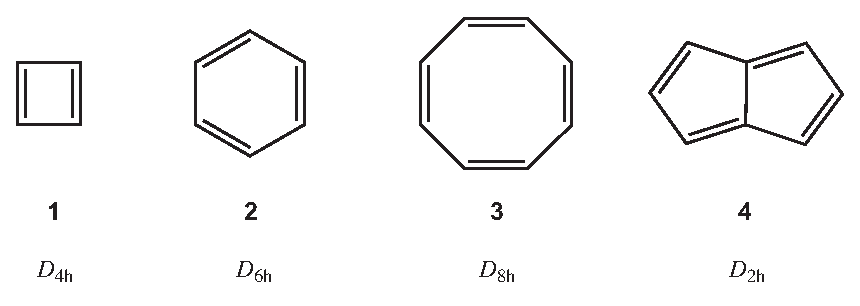
\includegraphics[scale=0.85]{orbopt/figures/compounds.eps}
\caption{Cyclobutadiene (\textbf{1}), benzene (\textbf{2}), cyclooctatetraene (\textbf{3}) and pentalene (\textbf{4}). Underneath the compound numbers the symmetry used for the respective compounds has been printed.}
\label{ch2.fig.compounds}
\end{figure}

Prior to any VB calculation, the geometry of the compounds had been optimized in the symmetry indicated in Figure \ref{ch2.fig.compounds}, using Restricted Hartree-Fock (RHF) with the \mbox{6-31G} basis set \cite{631g1,631g2}. The Valence Bond calculations, three per molecule, using the \textit{superci}, \textit{pert} and \textit{fock} options, were performed using delocalized $\sigma$ orbitals and strictly atomic $\pi$ orbitals, generated by a RHF calculation and an atomic SCF, respectively, all in the 6-31G basis. For all VB calculations, the DIIS option was switched on from the start. TURTLE's \textit{hybrid} option was used to separate the $\pi$ orbitals from each other and the $\sigma$ core. \textit{All} excitations were treated with perturbation, both for \textit{pert} and for \textit{fock}. In this case the \textit{fock} option can be used for the doubly occupied orbitals in the $\sigma$ core, because of the orthogonality of the $\pi$ orbitals to the $\sigma$ core. 

In Table \ref{ch2.tab.flat1} and \ref{ch2.tab.flat2} the results are presented. The total energies, presented below the name of each compound in the tables, was equal for all optimization methods for the first eight decimal places. Beneath the energies, for all methods the number of iterations, the total timings and the speed-up factors compared to regular Super CI are presented. In the case of the \textit{fock} option only the orbitals from the $\sigma$ core are optimized using the Fock algorithm; the $\pi$ orbitals are optimized using the \textit{pert} option in that case.

\begin{table}[htbp]
\caption{Below their names, the total energy of both molecules is presented. The number of iterations, timing per iteration and speed-up factors (compared to \textit{superci}) for butadiene and benzene.}
\begin{center}
\begin{tabular}{l c c c c c c}
\hline
&\multicolumn{3}{c}{\textbf{Butadiene}}&\multicolumn{3}{c}{\textbf{Benzene}}\\
&\multicolumn{3}{c}{(-153.59682368 au)}&\multicolumn{3}{c}{(-230.54408700 au)}\\
\textbf{Method}&\textbf{\# iter}&\textbf{sec/iter}&\textbf{speed-up}&\textbf{\# iter}&\textbf{sec/iter}&\textbf{speed-up}\\
\hline
\textit{superci}&8&73.0&1&8&2274.1&1\\
\textit{pert}&14&4.9&8&13&90.8&15\\
\textit{fock}&10&4.8&12&10&79.3&23\\
\end{tabular}
\label{ch2.tab.flat1}
\end{center}
\end{table}

\begin{table}[htbp]
\caption{Below their names, the total energy of both molecules is presented. The number of iterations, timing per iteration and speed-up factors (compared to \textit{superci}) for cyclooctatetraene and pentalene.}
\begin{center}
\begin{tabular}{l c c c c c c}
\hline
&\multicolumn{3}{c}{\textbf{Cyclooctatetraene}}&\multicolumn{3}{c}{\textbf{Pentalene}}\\
&\multicolumn{3}{c}{(-307.35606250 au)}&\multicolumn{3}{c}{(-306.14034868 au)}\\
\textbf{Method}&\textbf{\# iter}&\textbf{sec/iter}&\textbf{speed-up}&\textbf{\# iter}&\textbf{sec/iter}&\textbf{speed-up}\\
\hline
\textit{superci}&8&320106.0&1&8&47692.8&1\\
\textit{pert}&13&4704.2&42&14&1982.4&14\\
\textit{fock}&10&3857.0&66&12&1386.8&23\\
\end{tabular}
\label{ch2.tab.flat2}
\end{center}
\end{table}

For all molecules, the Super CI calculations take 8 iterations. Both in the \textit{fock} and in the \textit{pert} calculations more iterations are necessary to reach convergence. The approximation of the diagonal matrix element (Section \ref{ch2.sec.denominator}) seems to be beneficial for the calculation, because the number of iterations for \textit{fock} is smaller than for \textit{pert} in all four situations.

From the timings, it becomes clear that the \textit{fock} option is fruitful for this type of molecule, because the speed-up lies between 12 times for butadiene to 66 times for cyclooctatetraene compared to traditional Super CI. The difference between the speed-up of \textit{fock} and \textit{pert} is reasonable, but not as impressive as the difference between \textit{pert} and \textit{superci}. A drawback of the \textit{fock} option is the orthogonality condition that has to be met. 

Delocal VBSCF calculations, for which no examples have been presented here, do not suffer from this drawback, because in those calculations the doubly occupied orbitals will be orthogonal to each other, to the variably occupied orbitals and to the virtuals. However, most VB calculations in this thesis have been run with the \textit{hybrid} option, for which the \textit{fock} option is restricted to special cases, where the different \textit{hybrids} are orthogonal by symmetry.

\subsection{\label{ch2.sec.cyclopent}Second Example: The Cp-SiH Molecule}

For the work described in Chapter \chcyclopentadienyl\, a number of local VBSCF calculations have been performed to investigate the bonding mechanism of main group metal hydrides to cyclopentadienyl moieties. For details on the geometry optimization and the basis sets used, see Chapter \chcyclopentadienyl\ and reference \cite{budzelaar}. One of the molecules from that research is taken, the $\sigma$ bound \mbox{Cp-SiH} structure (Figure \ref{fig.cpsih}).
\begin{figure}[htdp]
\center
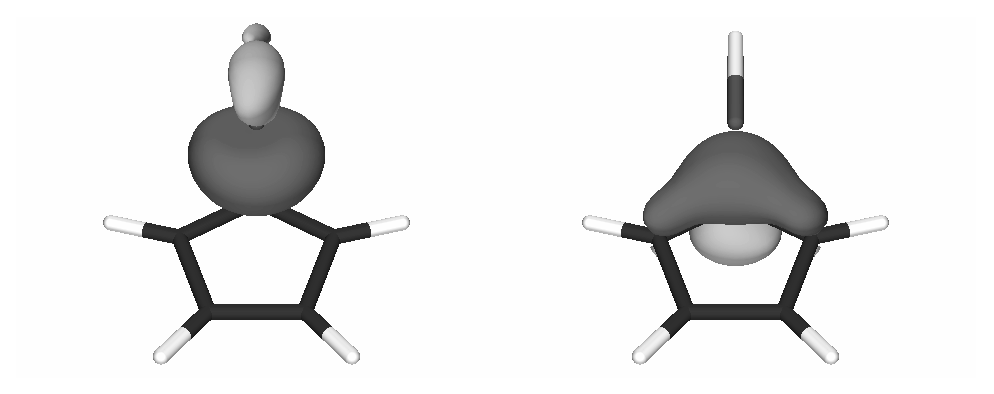
\includegraphics[scale=0.6]{orbopt/figures/sigma_sih.eps}
\caption{The $\sigma$ bound structure of Cp-SiH. Shown are the two singly occupied orbitals: the $sp$ hybridized orbital on SiH (left) and a $p$ orbital on the Cp-ring (right).}
\label{fig.cpsih}
\end{figure}
The calculation on this molecule forms a useful example for testing the additions to the optimization options, because the VBSCF process changes the orbitals drastically (in this case the total energy drops 0.86 Hartree between the initial and the final iteration). This is caused by the quality of the guess orbitals of which several are generated by hand instead of by a preceding Hartree-Fock calculation.

The molecule consists of two separate fragments, or \textit{hybrids} as they are referred to in TURTLE, \textit{i.e} the cyclopentadienyl part and the siliconhydride part. In these parts the doubly occupied orbitals are orthogonal to each other, to the variably occupied and virtual orbitals inside their \textit{hybrid}. However, the \textit{hybrids} are not necessarily orthogonal to one another. In this case the orbitals in the cyclopentadienyl \textit{hybrid} are not orthogonal to the orbitals in the siliconhydride \textit{hybrid} and therefore the \textit{fock} option cannot be used.

For the original calculations TURTLE's \textit{super} option, which ensures that only excitations to virtual (unoccupied) orbitals are included in Super CI, was used. Without the \textit{super} option excitations to partly occupied orbitals are included as well. The reason was that the excitations from occupied orbitals in one structure to a partly vacant orbital in the same or in an other structure resulted in convergence problems. For the specification of the \textit{pert} option via orbital classes, this means that only excitations from doubly to unoccupied orbitals \mbox{(doc-uoc)} and excitations from variably to unoccupied orbitals \mbox{(voc-uoc)} have to be tested, since excitations from doubly occupied to variably occupied \mbox{(doc-voc)} and from variably to variably occupied orbitals \mbox{(voc-voc)} are not used in this \textit{super} VBSCF calculation.

Besides the effect of the \textit{pert} option, the effect of the convergence helpers DIIS \cite{diis1,diis2} and level shifting \cite{level1,level2} was analyzed. In DIIS a successive set of iterations, of which each has an associated set of new orbitals and a gradient vector ($\mathbf{b}$), are used to guess the new orbitals. For more details and its use in TURTLE, see appendix III in \cite{koos1}. With the level shifter in TURTLE, the value of $\left < \Psi_0 | \mathbf{H} - E_0 | \Psi_0 \right >$ is lowered by a user specified amount during the diagonalization step. A useful value for the shifter, if any, is found by trial and error. DIIS, when applied, was used from the first iteration on. For the level shifter, when applied, only the value 1 was used. Furthermore, the convergence criterion was set to 1*10$^{-4}$ as maximum value for any of the Brillouin coefficients ($b_{ia}$, equation \ref{ch2.eq.superci}). This resulted in a total VB-energy which was, up to 5 decimal places, the same for all (converged) calculations: -481.44177 Hartree.

The results of the calculations are presented in Table \ref{ch2.tab.budzelaar}.
\begin{table}[htdp]
\caption{Timings in seconds of the VBSCF calculations on Cp-SiH (with the number of iterations between parenthesis). Three different optimization types were tested, regular Super CI, doc-uoc and doc-uoc/voc-uoc. With these different optimization types a combination of two convergence aids, DIIS and a level shifter (only for the \textit{pert} calculations) have been applied.}
\begin{center}
\begin{tabular}{l c c}
\hline
Type & no DIIS & DIIS \\
\hline
\textit{superci} & 3349 (11) & 2735 (9) \\ 
\textit{pert} doc-uoc & 1368 (99) & 324 (23)\\ 
\textit{pert} doc-uoc/voc-uoc & 1172 (98) & 316 (26)\\
\end{tabular}
\label{ch2.tab.budzelaar}
\end{center}
\end{table}
Without the convergence aid of a level shifter the calculations on this molecule with the \textit{pert} option switched on did not converge, while the regular Super CI calculation converged successfully in 11 iterations after 3349 seconds. Although the number of iterations needed to reach convergence is much larger than for a Super CI calculation, the total timings for the calculations with the \textit{pert} option are significantly lower. This is because the number of matrix elements necessary for \textit{pert} is much lower and therefore each iteration takes less time, but on the other hand information is discarded by leaving out matrix elements which results in (much) more iterations. 

Switching on DIIS appeared to be very beneficial for the \textit{pert} calculations, since it reduced the number of iterations roughly by a factor of four (Table \ref{ch2.tab.budzelaar}). For the \textit{superci} calculation DIIS was also advantageous: the calculation was shortened by almost 20\%.

\section{Conclusions}

Fock matrix elements, which can be calculated faster than Brillouin matrix elements, can be used for all excitations for which the orbital from which the excitation takes place (usually the doubly occupieds) and the orbital to which the excitation is, are orthogonal to each other and to the other orbitals. The other orbitals are allowed to be non-orthogonal to one another. In combination with the \textit{hybrid} option the \textit{fock} option can only be used when the doubly occupied orbitals in different \textit{hybrids} are orthogonal to all other orbitals.

When Fock matrix elements can be used, the calculation takes less time with the \textit{fock} than with the \textit{pert} option. However, the difference between \textit{fock} and \textit{pert} is not as impressive as the difference between \textit{pert} or \textit{fock} and \textit{superci}. Furthermore, the \textit{fock} option is not as generally applicable as the \textit{pert} option, because the latter does not require any orthogonality amongst the orbitals.

\section{Outlook}

In the theory section it has been shown that Brillouin matrix elements of the type $t \rightarrow a$ can be calculated from a series of inactive Fock matrix elements $F^{I}_{ta}$ and a set of second order cofactors (equation \ref{ch2.eq.ta_i7}). Although not implemented yet, computation time could be saved once it would be available in TURTLE. In that case, the construction of two separate Fock matrices is needed, $F^{I}_{ta}$ (for the inactive, or doubly occupied orbitals) and $F^{A}_{ta}$ (for the active, or variably occupied orbitals).

\section*{Appendix A: Cofactors}

A cofactor is a signed minor \cite{aitken}. A minor is created by removing one or more rows and columns from a determinant. Minors have the same sign as the original determinant from which they are derived. For a cofactor the sign depends on the position of the deleted row and column \cite{fokkeproef}. In this chapter the orbital overlap determinant, from which no rows and columns are removed, will be referred to as zeroth order cofactor. For a first order cofactor, obtained by removing one row and one column from the original determinant, the sign is $-1^{x+y}$, in which $x$ and $y$ are the indexes of the deleted row and column. For a second order cofactor, obtained by removing two rows and two columns from the original determinant, the sign is $-1^{x_1+x_2+y_1+y_2}$, in which $x_1$, $x_2$, $y_1$ and $y_2$ are the indexes of the deleted rows and columns. 

The overlap between two determinants can be expressed as  a zeroth order cofactor. The overlap of $\Delta_{1} = |ijkl \cdots n|$ with $\Delta_{2} = |ajkl \cdots n|$ for normalized orbitals is, \textit{e.g.}:
\begin{equation}
S_{12}^{(0)}=
\begin{array}{lllllll}
 &  i & j & k & l & \cdots & n \\
 a &  \multicolumn{1}{|l}{s_{ia}} & s_{ja}  & s_{ka} & s_{la} & & \multicolumn{1}{l|}{ s_{na} } \\
 j & \multicolumn{1}{|l}{s_{ij}} & 1 & s_{kj} & s_{lj} & & \multicolumn{1}{l|}{s_{nj}} \\
 k & \multicolumn{1}{|l}{s_{ik}} & s_{jk} & 1 & s_{lk} & & \multicolumn{1}{l|}{s_{nk}} \\
 l & \multicolumn{1}{|l}{s_{il}} & s_{jl} & s_{kl} & 1 & & \multicolumn{1}{l|}{s_{nl}} \\
 \vdots & \multicolumn{1}{|l}{ } &   &   & & \ddots & \multicolumn{1}{l|}{\vdots} \\
 n & \multicolumn{1}{|l}{ s_{in}} & s_{jn} & s_{kn} & s_{ln} & \cdots & \multicolumn{1}{l|}{1}
\end{array},\\
\label{ch2.eq.zocofac}
\end{equation}
in which the $s_{xy}$ elements stand for the orbital overlaps, \textit{i.e.} $\left < x | y \right >$. Along the rows and columns orbital labels are shown for readability. In the notation $S_{12}^{(0)}$, the superscript $(0)$ indicates that this is a zeroth order cofactor. The subscript $12$ indicates that the cofactor is constructed from overlaps of orbitals in determinant $\Delta_1$ with those from determinant $\Delta_2$.

A first order cofactor is derived from the zeroth order cofactor by removing one row and one column. So, when the column labeled $i$ and the row labeled $a$ are removed, the first order cofactor $S_{12}^{(i,a)}$ emerges:
\begin{equation}
S_{12}^{(i,a)} =
\begin{array}{lllllll}
 &  \hskip 2.0 pt \hbox{\lower 120pt\hbox{\vrule height128pt width 1.0pt}}\hskip-3.0pt i & j & k & l & \cdots & n \\
\noalign{\vskip-115pt}
 a &  \multicolumn{1}{|l}{s_{ia}} & s_{ja}  & s_{ka} & s_{la} & & \multicolumn{1}{l|}{ s_{na} } \\
\noalign{\vskip-8pt}
\multispan7\hbox{\vrule  height 1.0 pt width164pt}\cr
\noalign{\vskip 7pt}
  j & \multicolumn{1}{|l}{s_{ij}} & 1 & s_{kj} & s_{lj} & & \multicolumn{1}{l|}{s_{nj}} \\
 k & \multicolumn{1}{|l}{s_{ik}} & s_{jk} & 1 & s_{lk} & & \multicolumn{1}{l|}{s_{nk}} \\
 l & \multicolumn{1}{|l}{s_{il}} & s_{jl} & s_{kl} & 1 & & \multicolumn{1}{l|}{s_{nl}} \\
 \vdots & \multicolumn{1}{|l}{ } &   &   & & \ddots & \multicolumn{1}{l|}{\vdots} \\
 n & \multicolumn{1}{|l}{ s_{in}} & s_{jn} & s_{kn} & s_{ln} & \cdots & \multicolumn{1}{l|}{1}
\end{array}.\\
\label{ch2.eq.focofac}
\end{equation}
Since orbital $i$ is in the first column and orbital $a$ on the first row, the sign of the cofactor does not change because $-1^{(1+1)} = +1$.

When the columns labeled $i$ and $k$ and the rows labeled $a$ and $l$ are removed from $S_{12}^{(0)}$ the second order cofactor $S_{12}^{(i,k,a,l)}$ is generated:
\begin{equation}
S_{12}^{(i,k,a,l)} =
\begin{array}{lllllll}
 &  \hskip 2.0 pt \hbox{\lower 120pt\hbox{\vrule height128pt width 1.0pt}}\hskip-3.0pt i & j & \hskip 2.0 pt \hbox{\lower 120pt\hbox{\vrule height128pt width 1.0pt}}\hskip-3.0pt k & l & \cdots & n \\
\noalign{\vskip-115pt}
 a &  \multicolumn{1}{|l}{s_{ia}} & s_{ja}  & s_{ka} & s_{la} & & \multicolumn{1}{l|}{ s_{na} } \\
 \noalign{\vskip-8pt}
\multispan7\hbox{\vrule  height 1.0 pt width164pt}\cr
\noalign{\vskip 7pt}
 j & \multicolumn{1}{|l}{s_{ij}} & 1 & s_{kj} & s_{lj} & & \multicolumn{1}{l|}{s_{nj}} \\
 k & \multicolumn{1}{|l}{s_{ik}} & s_{jk} & 1 & s_{lk} & & \multicolumn{1}{l|}{s_{nk}} \\
 l & \multicolumn{1}{|l}{s_{il}} & s_{jl} & s_{kl} & 1 & & \multicolumn{1}{l|}{s_{nl}} \\
 \noalign{\vskip-8pt}
\multispan7\hbox{\vrule  height 1.0 pt width164pt}\cr
\noalign{\vskip 7pt}
 \vdots & \multicolumn{1}{|l}{ } &   &   & & \ddots & \multicolumn{1}{l|}{\vdots} \\
 n & \multicolumn{1}{|l}{ s_{in}} & s_{jn} & s_{kn} & s_{ln} & \cdots & \multicolumn{1}{l|}{1}
\end{array}.\\
\label{ch2.eq.socofac}
\end{equation}
In this second order cofactor the sign changes, because the position of the orbitals is: $i$ in the first and $k$ in the third column, $a$ on the first and $l$ on the fourth row. This makes $-1^{(1+3+1+4)} = -1$.

\bibliography{orbopt}
\bibliographystyle{../main/achemso}

\setcounter{chapter}{2}
\setcounter{NAT@ctr}{0}
\chapter{Dissociation of Polar Bonds in the Gas Phase and in Solution: A Valence Bond Approach}
\footnotetext{Partly published in ``On the Interpretation of Valence Bond Wavefunctions'', \mbox{R. W. A. Havenith}, \mbox{J. H. van Lenthe}, \mbox{L. W. Jenneskens} and \mbox{J. J. Engelberts}, \textit{Faraday Discuss.} \textbf{2007}, \textsl{135}, 299-308.}
\label{chap_dissociation}

\hyphenation{chlo-ro-me-thane pro-noun-ced mol-e-cules}

\ifthenelse{\boolean{wholethesis}}{\relax}{\begin{center}\textit{Generated on \today\ at \currenttime}\end{center}}

\noindent\textbf{Abstract:} The influence of a solvent on the dissociation behavior of four chlorine containing compounds with varying polarity, chloromethane, \textit{tert}-butylchloride, chlorosilane and trimethylsilylchloride, is analyzed with VB in conjunction with the Polarizable Continuum Model (PCM), in which the solvent is represented as a homogeneous medium that is characterized by its dielectric constant. VB calculations without solvent effects show that all four molecules dissociate to a radical chlorine atom and an alkyl/silyl radical. When water as a solvent is mimicked by PCM \textit{tert}-butylchloride, chlorosilane and trimethylsilylchloride dissociate to ions, whereas chloromethane is hardly influenced by the solvating medium. Homolytic bond dissociation to radicals occurs.

In the last part of this chapter it is shown that the C--H orbitals, albeit separated by one bond from the active center, are involved in the reaction via hyperconjugation which stabilizes the \textit{tert}-butyl cation. 

\clearpage

\section{Introduction}

\lettrine{\initial{C}}{}hemical bonds can be classified into several categories, like covalent (polar and apolar), ionic, and metallic bonds. An apolar covalent bond is a chemical bond, in which atoms share equally electrons in order to obtain a noble gas configuration. An example is H$_2$ (Figure \ref{ch3.fig.h_twee}), where each hydrogen atom contributes one electron to the bond, resulting in a noble gas configuration (He) for both of them.
\begin{figure}[ht]
\center
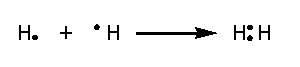
\includegraphics{dissociation/figures/h_twee.eps}
\caption{Two hydrogen atoms forming a H$_2$ molecule (Lewis structure on the right).}
\label{ch3.fig.h_twee} 
\end{figure}

If one electron is transferred from one atom to the other, which results in two oppositely charged ions, the bond is completely ionic, as in \textit{e.g.} NaCl (Figure \ref{ch3.fig.nacl}). The ions remain bound only by electrostatic interactions. 
\begin{figure}[ht]
\center
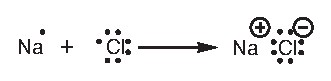
\includegraphics{dissociation/figures/nacl.eps}
\caption{A sodium and a chlorine atom forming a NaCl ``molecule''.}
\label{ch3.fig.nacl}
\end{figure}

In between these two extremes is the polar bond, which possesses mixed covalent and ionic character. Hydrogenchloride (HCl) is such a molecule (Figure \ref{ch3.fig.hcl}). Although hydrogen and chlorine share electrons the electron pair will be located more on the chlorine than on the hydrogen atom, due to the higher electronegativity of chlorine.
\begin{figure}[ht]
\center

\includegraphics{dissociation/figures/hcl.eps}
\caption{A hydrogen and a chlorine atom forming a HCl molecule.}
\label{ch3.fig.hcl}
\end{figure}

Shaik \textit{et al.} have defined a fourth bond type, the charge-shift bond \cite{cs1,cs2}. They define this bond as a fundamental bond type for those electron pair bonds that are neither covalent, nor ionic in nature. Characteristic for charge-shift bonds are a large charge-shift resonance energy ($RE_{CS}$) and a relatively small contribution of the covalent structure ($D_\mathrm{cov}$). It is, however, not limited to molecules that can be considered as ``in between'' covalent and ionic in nature. The bond in fluorine (F$_2$, Figure \ref{ch3.fig.f_twee}), a homopolar, homonuclear diatomic molecule, is classified as a charge-shift bond.
\begin{figure}[h]
\center
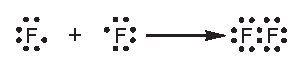
\includegraphics{dissociation/figures/f_twee.eps}
\caption{Two fluorine atoms forming a F$_2$ molecule.}
\label{ch3.fig.f_twee} 
\end{figure}

In this chapter, the dissociation of polar bonds is studied with the Valence Bond method, in which the wave function can be expressed in covalent and ionic structures. In reference \cite{interpret} a discussion on the assumed equivalence of Lewis and Valence Bond structures is presented. As an introduction dissociation curves for H$_2$ (covalent bond), the ``NaCl'' molecule (ionic bond) and F$_2$ (charge-shift bond) in the gas phase are presented to show the differences in dissocation of these chemical bonds.

The central question in this chapter is: How does the dissociation change when the parameters influencing the bond, like the atoms involved, the surrounding medium and different functional groups, are changed?

To obtain answers to this question, the dissociation pathway of several polar bonds with different polarity and in different media, \textit{viz.} vacuum and water, will be studied.  The set of molecules consists of chloromethane (\textbf{1}), which possesses a typical polar C--Cl bond, \textit{tert}-butylchloride (\textbf{2}) and their silicon analogues chlorosilane (\textbf{3}) and trimethylsilylchloride (\textbf{4}) (Figure \ref{ch3.fig.compounds}).  
\begin{figure}[htbp]
\begin{center}
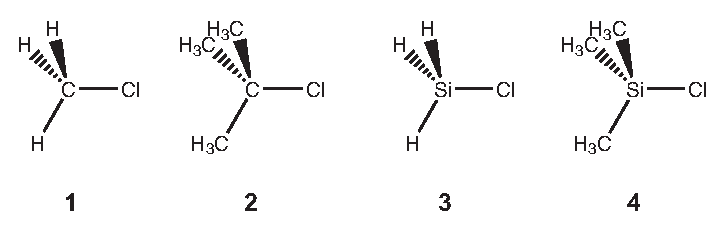
\includegraphics{dissociation/figures/compounds.eps}
\end{center}
\caption{Chloromethane (CH$_3$Cl, \textbf{1}), \textit{tert}-butylchloride
(C(CH$_3$)$_3$Cl, \textbf{2}), chlorosilane (SiH$_3$Cl, \textbf{3}) and trimethylsilanechloride
(Si(CH$_3$)$_3$Cl, \textbf{4})}
\label{ch3.fig.compounds}
\end{figure} 
The bond that will be broken is the C/Si--Cl bond. The silicon analogues have been selected because silicon has a much lower electronegativity than carbon (compare the Pauling electronegativity of 1.90 for silicon with 2.55 for carbon \cite{handbook}). The influence this difference may have on the dissociation behavior of carbon and silicon compounds is analyzed. Furthermore, the influence of the difference between hydrogen atoms and methyl-groups on the dissocation will be compared. Methyl-groups exert an electron donating character \cite{mcmurry}, compared to hydrogen. Besides, the methyl-hydrogens might exert an effect on the dissociation process through hyperconjugation \cite{march}, not present in the hydrogen substituted compounds. Orbitals on the C--H bonds of the methyl-groups, which are several bond lengths separated from the tertiary carbon atom, may still have an influence on it, and hence on the dissociation behavior. 

The alteration of the dissociation behavior by different surrounding media will be investigated using calculations performed with the Polarizable Continuum Model (PCM) \cite{pcm1,pcm2} which accounts for solvation effects in its simplest form: the solvent is represented as a homogeneous medium that is characterized by its dielectric constant without further explicit molecular interactions between the solvent molecules and the solute. 

The Valence Bond wave functions used to describe the dissociation behavior of these molecules contain the three structures presented in Figure \ref{ch3.fig.structures}.
\begin{figure}[htbp]
\begin{center}
\includegraphics{dissociation/figures/structures.eps}
\end{center}
\caption{The Valence Bond structures, a covalent (\textbf{a}) and two ionic (\textbf{b} and \textbf{c}) structures (M=C or Si; R=H or CH$_3$).}
\label{ch3.fig.structures}
\end{figure}
An indication of the polarity of the bond is given by weights attributed to the structures \cite{coulson}. 

For all four compounds dissociation energies from prior VB calculations are available. Lauvergnat \textit{et al.} \cite{lauvergnat} performed VBSCF \cite{vbscf1,vbscf2} and BOVB \cite{bovb1,bovb2,bovb3} calculations on \textbf{1} and \textbf{3} in the gas phase. They concluded that BOVB is necessary to obtain a dissociation energy that is close to the experimental value (334.3 kJ/mol (BOVB) \textit{vs} 365.3 kJ/mol (experimental) for \textbf{1} and 425.5 kJ/mol (BOVB) \textit{vs} 463.2 kJ/mol (experimental) for \textbf{3}), but that VBSCF calculations sufficed to obtain qualitatively correct results.  Song \textit{et al.} \cite{song} have performed test calculations with VB in conjunction with PCM, to which they refer as VBPCM, on \textit{tert}-butylchloride (\textbf{2}) with frozen C--H bond orbitals. The latter study confirmed the heterolytic dissociation of \textbf{2} in water as a solvent. Su \textit{et al.} \cite{psu} have investigated \textbf{2} and \textbf{4} in the gas phase and with VBPCM. They have concluded that the C--Cl and Si--Cl bonds are of different natures. While C--Cl is considered to be a covalent bond, Su \textit{et al.} consider Si--Cl to be of the category of charge-shift bonds. The reasoning behind this is the significantly higher resonance energy in the silicon case. Our results will further extend the study of the dissociation of polar, \textit{cq.} charge-shift bonds.

The research is split-up in four parts.  In the first part, Valence Bond results of the dissociation of a purely covalent (H$_2$), a purely ionic (NaCl) and a charge-shift bond (F$_2$) in the gas phase will be presented to illustrate the differences between these three in dissociation, \textit{i.e.} H$_2$ for covalent, NaCl for ionic and F$_2$ for charge-shift. Secondly, compounds \textbf{1}-\textbf{4} are investigated in the gas phase using Valence Bond theory. Thirdly, the effect of water as a solvent on the dissociation pathways of these compounds is analyzed with PCM. Finally, it will be shown that freezing of orbitals, in particular C--H orbitals, may inadvertently affect the results of the calculation. It is shown that the observed effect is linked to contributions of the phenomenon of hyperconjugation.

\section{Dissociation of H$_2$, NaCl and F$_2$ in the Gas Phase}

In the H$_2$ molecule, both hydrogen atoms contribute one electron to the bond. The two electrons can be arranged in four ways, expressed in the three Lewis structures:
\begin{equation}
\nonumber
\mathrm{H-H\ \ \equiv \ \ H^{\bullet}\ \ H^{\bullet}\ \ +\ \ H^{+}\ \ H^{-}\ \ +\ \ H^{-}\ \ H^{+}}.
\end{equation}
Both electrons can be located on their individual atoms ($\mathrm{H^{\bullet}\ \ H^{\bullet}}$) or both electrons can be located on one of the hydrogen atoms ($\mathrm{H^{+}\ \ H^{-}}$ and $\mathrm{H^{-}\ \ H^{+}}$). To analyze the dissociation of the H$_2$ bond theoretically, it is expressed in the three VB structures:
\begin{equation}
\nonumber
\Psi_{\mathrm{H_2}} = c_1\cdot [\mathrm{H}^\bullet \mathrm{H}^\bullet] + c_2 \cdot [\mathrm{H}^{+}\mathrm{H}^{-}] + c_3 \cdot [\mathrm{H}^{-}\mathrm{H}^{+}]. 
\end{equation}
Energies for the total wave function and the structures separately are calculated at different interatomic distances. Because $[\mathrm{H}^{+}\mathrm{H}^{-}]$ and $[\mathrm{H}^{-}\mathrm{H}^{+}]$ are equivalent their corresponding coefficients will be equal ($c_2 = c_3$).  

In Figure \ref{ch3.fig.h2_c} the dissociation path for H$_2$ is shown. The total energy curve ($E_\mathrm{tot}^\mathrm{gas}$) and the energy curves of the covalent ($E_\mathrm{cov}^\mathrm{gas}$) and ionic ($E_\mathrm{ion}^\mathrm{gas}$) structures separately are presented. 
\begin{figure}[htbp]
\begin{center}
\includegraphics[scale=0.6]{dissociation/figures/h2_g.eps}
\end{center}
\caption{The dissociation curve of H$_2$ in the gas phase. $E_\mathrm{tot}^\mathrm{gas}$ is the total VB energy, $E_\mathrm{cov}^\mathrm{gas}$  and $E_\mathrm{ion}^\mathrm{gas}$ are the energies of the covalent $[\mathrm{H^\bullet H^\bullet}]$ and ionic $[\mathrm{H^{+}H^{-}}]$ structures separately. The minima are shown in parenthesis.}
\label{ch3.fig.h2_c}
\end{figure}
The total and covalent curves practically coincide over the whole range. This indicates the covalent character of the bond in H$_2$. For the covalent structure the weight is at least 0.8 over the whole dissociation range.

Typical for the ionic and covalent curves is that they are easily distinguishable by their shape, at least in the curves presented here. The value of $E_\mathrm{ion}^\mathrm{gas}$ increases with increasing bonding distance from the minimum energy distance to higher distances. In the covalent curves the increase in $E_\mathrm{cov}^\mathrm{gas}$ from the minimum in energy going to larger distances stops at distances roughly varying from 2.5 to 4.0 \AA. An explanation for the gradual increase of the ionic curves, not seen in either the covalent or neutral curves, can be found in electrostatics (Coulomb attraction): when two oppositely charged bodies, in this case atoms or molecular fragments, are separated, the potential energy increases inversely proportional to the separation distance ($\frac{1}{r}$).

In analogy with $\Psi_{\mathrm{H_2}}$, a three structure VB wave function for the NaCl ``molecule'' is constructed:
\begin{equation}
\nonumber
\Psi_{\mathrm{NaCl}} = c_1\cdot [\mathrm{Na}^\bullet \mathrm{Cl}^\bullet] + c_2 \cdot [\mathrm{Na}^{+}\mathrm{Cl}^{-}] + c_3 \cdot [\mathrm{Na}^{-}\mathrm{Cl}^{+}]. 
\end{equation}
Dissociation curves for $\Psi_{\mathrm{NaCl}}$ are presented in Figure \ref{ch3.fig.nacl_c}.
\begin{figure}[hbtp]
\begin{center}
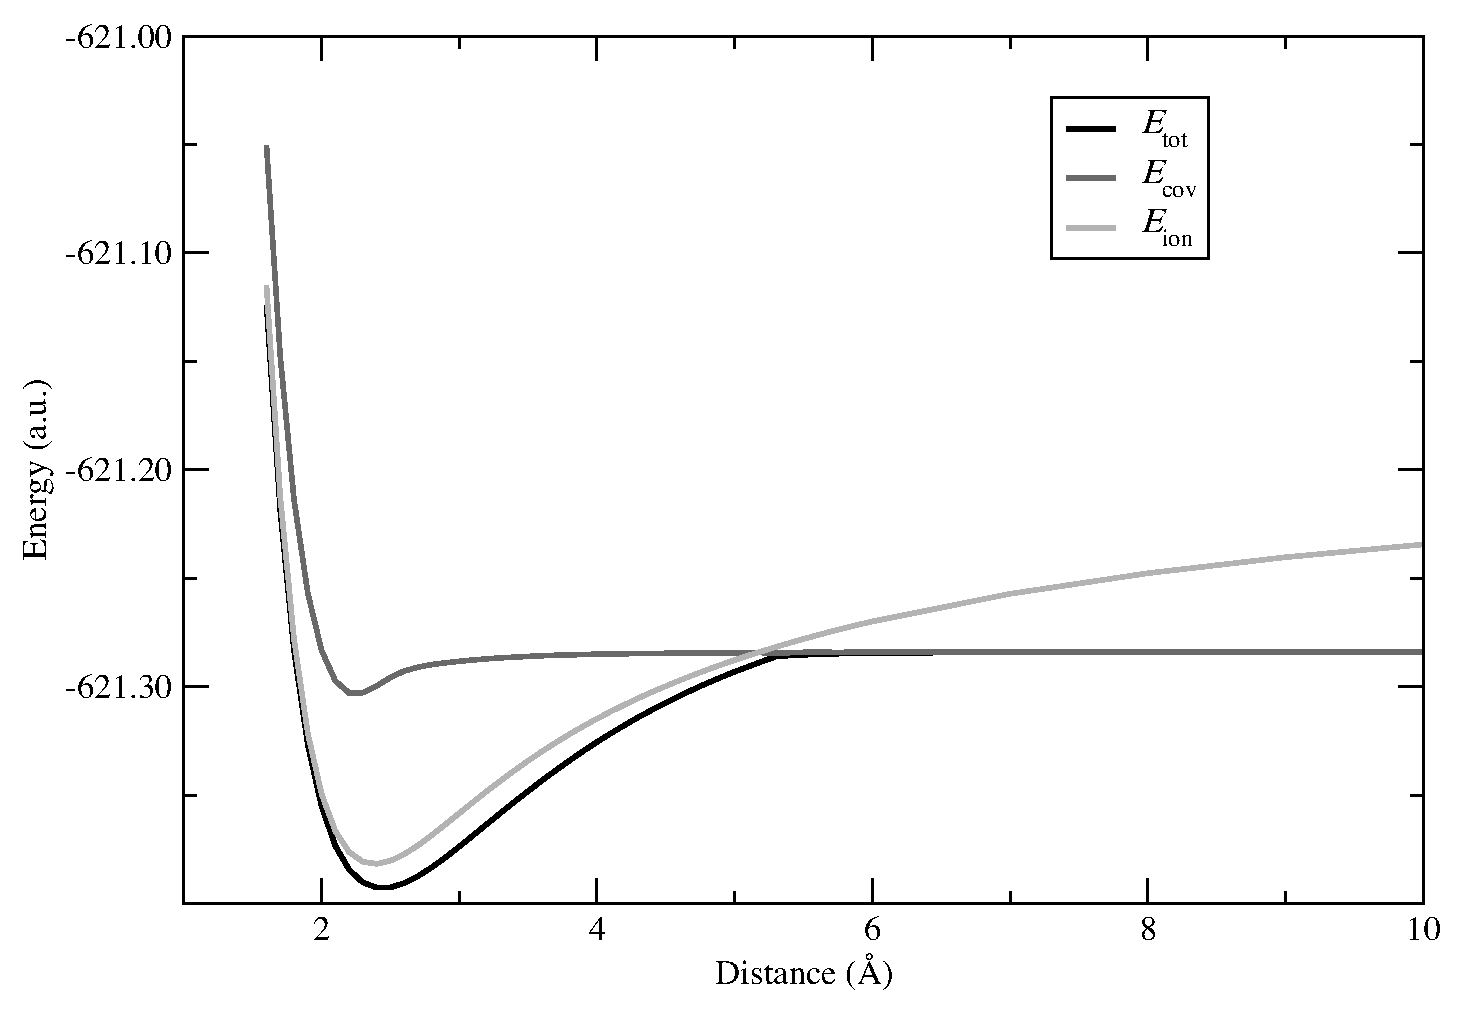
\includegraphics[scale=0.6]{dissociation/figures/nacl_g.eps}
\end{center}
\caption{The dissociation curve of the NaCl ``molecule'' in the gas phase. $E_\mathrm{tot}^\mathrm{gas}$ is the total VB energy, $E_\mathrm{cov}^\mathrm{gas}$  and $E_\mathrm{ion}^\mathrm{gas}$ are the energies of the covalent $[\mathrm{Na^\bullet Cl^\bullet}]$ and ionic $[\mathrm{Na^{+}Cl^{-}}]$ structures separately. The minima are shown in parenthesis.}
\label{ch3.fig.nacl_c}
\end{figure}
The curve for the $[\mathrm{Na}^{-}\mathrm{Cl}^{+}]$ structure has been omitted, because its energy is approximately 0.5 a.u. higher than for the other two structures over the whole range and its contribution to the wave function is negligible ($c_3 \approx 0$). Nevertheless, it is included in $\Psi_{\mathrm{NaCl}}$ to keep the general expression of the wave functions, \textit{i.e.} built from three structures, equal for all molecules in this chapter:
\begin{equation}
\nonumber
\Psi_{\mathrm{AB}} = c_1\cdot [\mathrm{A}^\bullet \mathrm{B}^\bullet] + c_2 \cdot [\mathrm{A}^{+}\mathrm{B}^{-}] 
+ c_3 \cdot [\mathrm{A}^{-}\mathrm{B}^{+}],
\end{equation}
in which $\mathrm{A}$ and $\mathrm{B}$ can be atoms or molecular fragments (structures \textbf{a}, \textbf{b} and \textbf{c} in Figure \ref{ch3.fig.structures}).

Like for the other two molecules, a three structure VB wave function is constructed for F$_2$:
\begin{equation}
\nonumber
\Psi_{\mathrm{F_2}} = c_1\cdot [\mathrm{F}^\bullet \mathrm{F}^\bullet] + c_2 \cdot [\mathrm{F}^{+}\mathrm{F}^{-}] + c_3 \cdot [\mathrm{F}^{-}\mathrm{F}^{+}]. 
\end{equation}
In analogy with H$_2$, the coefficients $c_2$ and $c_3$ are equal. The dissociation curves are presented in \ref{ch3.fig.f2_c}.
\begin{figure}[hbtp]
\begin{center}
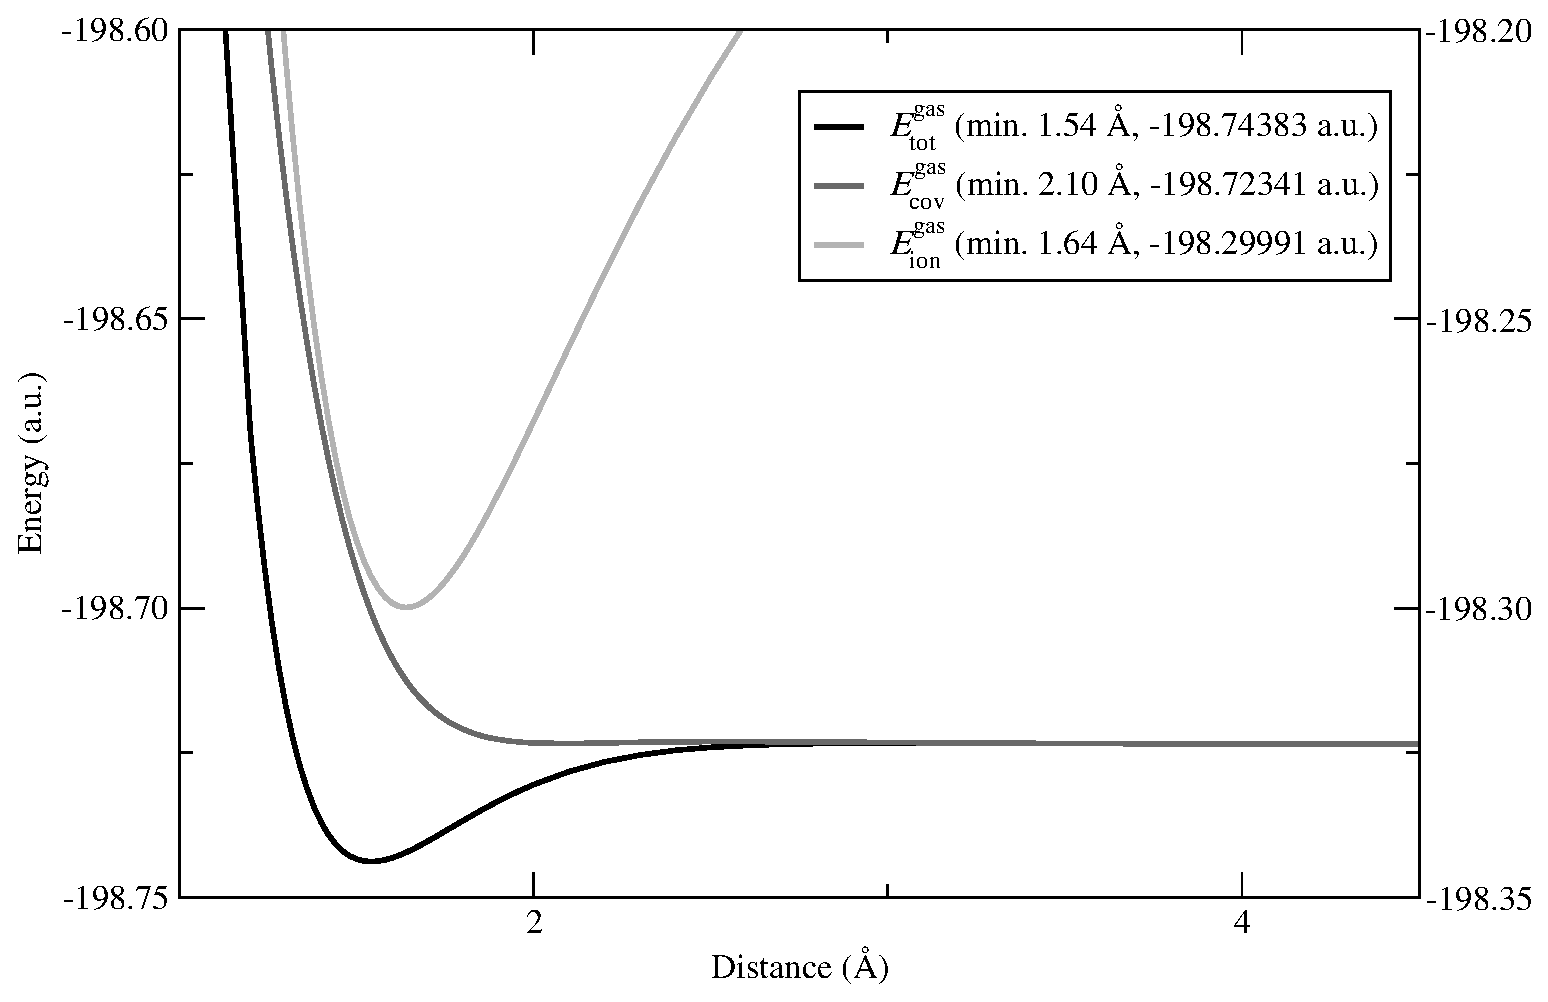
\includegraphics[scale=0.6]{dissociation/figures/f2_g.eps}
\end{center}
\caption{The dissociation curve of F$_2$ in the gas phase. $E_\mathrm{tot}^\mathrm{gas}$ is the total VB energy, $E_\mathrm{cov}^\mathrm{gas}$ is the curve of the covalent $[\mathrm{F^\bullet F^\bullet}]$ structure. The ionic curve with energy $E_\mathrm{ion}^\mathrm{gas}$ of the ionic structure  $[\mathrm{F}^{+}\mathrm{F}^{-}]$ is shifted by 0.4 a.u. to make it visible in the figure. Its energy scale is shown on the right hand side of the graph. The minima are shown in parenthesis.}
\label{ch3.fig.f2_c}
\end{figure}
The curve for the ionic structure ($E_\mathrm{ion}^\mathrm{gas}$) has been shifted by 0.4 a.u. in Figure \ref{ch3.fig.f2_c} because it is lying much higher than the curve for the total energy $E_\mathrm{tot}^\mathrm{gas}$ and hence would not have been visible, otherwise. The energy scale for the ionic structure is shown on the right hand side of the graph.

For H$_2$, the total energy curve practically coincides with the covalent curve (Figure \ref{ch3.fig.h2_c}), indicating that the covalent VB structure roughly corresponds to the bonding picture. The weight of the structure in the total wave function, as introduced by Chirgwin and Coulson \cite{chirgwin}, is 0.80 around the equilibrium distance. Charge-shift resonance energy, \textit{i.e.} the energy difference between the most stable structure (lowest in energy) and the total energy ($RE_{CS}$ \cite{cs1}), is 0.011 a.u. 

In the case of NaCl, the total energy curve coincides with the ionic curve around the equilibrium distance (Figure \ref{ch3.fig.nacl_c}), indicating that the ionic VB structure roughly corresponds to the bonding picture. This is further corroborated by the weight of the ionic structure at equilibrium distance (0.70) and the low resonance energy (0.025 a.u.).

For F$_2$, the covalent curve is lying much higher in energy than the total energy curve, while the ionic curve is even higher. The latter curve has been shifted down by 0.4 a.u. to make its shape visible in Figure \ref{ch3.fig.f2_c}. The covalent curve is lying above the energy level for two separate fluorine radicals and hence the covalent structure is non bonding in itself. Neither the covalent, nor the ionic structure represents the bonding, but rather the combination of the two does. Although the weight for the covalent structure is rather high (0.84) like for H$_2$, the high resonance energy (0.047) compared to H$_2$ suggests that the bond is rather different than a typical covalent bond. Shaik \textit{et al.} therefore classify this bond as of the charge-shift type \cite{cs1,cs2}.

An important difference between the curves of H$_2$ and NaCl is that in the latter case the covalent and ionic curves cross. At infinite distance the atoms Na and Cl are neutral, both having an odd number of electrons (Na 11 and Cl 17). There, the covalent description prevails, characterized by the coincidence of the $E_\mathrm{tot}^\mathrm{gas}$ and $E_\mathrm{cov}^\mathrm{gas}$ curves and the weight of 1.00 for the covalent structure. At equilibrium distance (R=2.4 \AA) both atoms roughly have a noble gas configuration (Na$^{+}$ = [Ne] and Cl$^{-}$ = [Ar]). At that point the $[\mathrm{Na}^{+}\mathrm{Cl}^{-}]$ structure forms the bonding picture, indicated by the small difference between $E_\mathrm{tot}^\mathrm{gas}$ and $E_\mathrm{ion}^\mathrm{gas}$ and its high weight of 0.70. In between those two points lies the crossing of the covalent and ionic curves, which occurs around 5.2 \AA. Although at that distance the energies of the two structures are the same, the difference in charge distribution is large: in the covalent case the atoms are neutral, while in the ionic case sodium is positively charged and chlorine negatively charged. In a VB calculation at a distance just below the crossing point distance the weight of the ionic structure is almost 0.90. However, at larger distances the weight of the ionic structure rapidly decreases to zero.

Another difference is the shape of the curves for the total energy ($E_\mathrm{tot}^\mathrm{gas}$): the steady increasing character for NaCl between 2.4 and 5.2 \AA, caused by the relative importance of the ionic structure, is absent in the curve for H$_2$, which rises quite rapidly to the energy level of two separate hydrogen atoms between 0.8 and roughly 2.5 \AA. So, it is expected that for bonds with ionic character, the total energy curve will exhibit more ``Coulombic character'' compared to covalent bonds. 

In the following section, the shapes and positions of the curves for \textbf{1}-\textbf{4} in the gas phase will be compared with each other and with H$_2$ and NaCl (the two examples mentioned above).

\section{\label{ch3.sec.gasphase}Gas Phase Dissociation of C/Si-Cl Bonds}

\subsection{Computational Methods}

Points on the dissociation path have been calculated with an interspacing of 0.1 \AA\ between 1.4 and 10.0 \AA\ for the \mbox{M--Cl} bond  (step \textit{1} in Figure \ref{ch3.fig.scheme1}). The other bond lengths and bond angles were optimized in $C_\mathrm{3v}$ symmetry using \mbox{GVB/6-31G*} \cite{gvb1,gvb2,gvb3,gvb4}, in which the \mbox{M--Cl} $\sigma$ and \mbox{M--Cl} $\sigma^{*}$ bonds were correlated.
\begin{figure}[htb]
\begin{center}
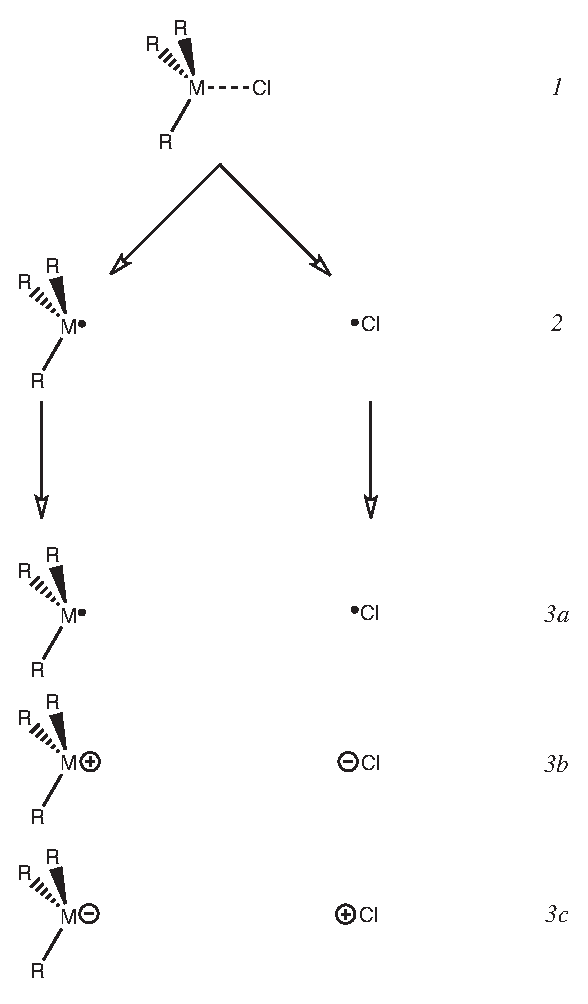
\includegraphics{dissociation/figures/scheme1.eps}
\end{center}
\caption{The three steps to generate dissociation curves: \textit{1.} Geometry optimization at fixed M--Cl (dashed) bonds. \textit{2.} Generation of start-up orbitals on radical fragments. \textit{3.} Valence Bond calculations on the three Lewis structures together (\textit{3a} + \textit{3b} + \textit{3c}).} 
\label{ch3.fig.scheme1}
\end{figure}
After these geometry optimizations start-up orbitals were generated on the R$_3$M$^{\bullet}$ and Cl$^{\bullet}$ fragments separately at the \mbox{RHF/6-31G*} level (step \textit{2} in Figure \ref{ch3.fig.scheme1}).  With these orbitals the Valence Bond wave functions containing the covalent (\textit{3a}) and both ionic (\textit{3b} and \textit{3c}) VB structures were constructed. The valence orbitals were subsequently optimized at the \mbox{VBSCF/6-31G*} level \cite{vbscf1,vbscf2}, while the core orbitals were frozen at their \mbox{RHF/6-31G*} levels.
Through the use of the local VBSCF model the valence orbitals were optimized on both the R$_3$M and Cl fragments separately; basis functions of the other fragment were not allowed to mix in, keeping the orbitals expressed in basis functions of a single fragment. All calculations were performed with TURTLE \cite{turtle} as implemented in GAMESS-UK \cite{gamess}.

\subsection{Results and Discussion}

The optimal M--Cl bond lengths ($R_\mathrm{eq}$) and the corresponding dissociation energies ($E_\mathrm{dis}^\mathrm{gas}$) are shown in Table \ref{ch3.tab.optimal}. $E_\mathrm{dis}^\mathrm{gas}$ is the difference between the lowest energy (at equilibrium) and the energy at 10 \AA. The optimal VB M--Cl bond lengths are obtained by a three-point fit through the three lowest points around the equilibrium. This process is needed, because the GVB minimum is not exactly equal to the VBSCF minimum. Since the orbitals in VBSCF are kept localized on either of the two fragments, the minima differ slightly. With these fitted minima, a new geometry optimization in which the M--Cl bond is kept constant at the interpolated optimal distance, while the other bonds and angles are optimized, was performed. This geometry was used in the VB calculations of which the VB energy values are presented in Table \ref{ch3.tab.optimal}. Next to our $E_\mathrm{dis}^\mathrm{gas}$ values, the corresponding values from literature and experimental values \cite{lauvergnat,psu} are shown. In the last column, the charge-shift resonance energy ($RE_{CS}$ \cite{cs1}) is presented. This is the difference between the energy of the most stable structure at equilibrium distance and the total energy. 
\begin{table}[hbt]
\center
\caption{The VB dissociation energy $E_\mathrm{dis}^\mathrm{gas}$, literature data \cite{lauvergnat,psu}, optimal M--Cl bond lengths and the resonance energy for charge-shift bonds ($RE_{CS}$) \cite{cs1}. $^\mathrm{a}$ 404.2 kJ/mol is computed with VBSCF with delocalized orbitals that  are not restricted to either the chlorine, or the trimethylsilyl fragment.}  
\begin{tabular}{|l|c|c|c|c|c|}
\hline
Compound & \multicolumn{3}{c|}{$E_\mathrm{dis}^\mathrm{gas}$ (kJ/mol)} & $R_\mathrm{eq}$ (\AA) & $RE_{CS}$ \\
\hline
&\multicolumn{1}{c|}{this} & \multicolumn{1}{c|}{earlier} & \multicolumn{1}{c|}{exp.} & (M--Cl length) & (kJ/mol) \\
&\multicolumn{1}{c|}{work} & \multicolumn{1}{c|}{VB calculations} & \multicolumn{1}{c|}{} & & \\
\hline
CH$_3$Cl (\textbf{1})& 260.9 & 255.6 \cite{lauvergnat} & 365.3 \cite{lauvergnat} & 1.894 & 179.9\\
C(CH$_3$)$_3$Cl (\textbf{2}) & 251.3 & 245.6 \cite{psu} & 360.7 \cite{psu} & 1.935 & 183.6\\
SiH$_3$Cl (\textbf{3})& 335.5 & 331.1 \cite{lauvergnat} & 463.2 \cite{lauvergnat} & 2.154 & 266.4\\
Si(CH$_3$)$_3$Cl (\textbf{4}) & 371.5 & 404.2$^\mathrm{a}$ \cite{psu} & --- & 2.175 & 310.4\\
\hline
\end{tabular}
\label{ch3.tab.optimal}
\end{table}
Our calculated dissociation energies for \textbf{1}, \textbf{2} and \textbf{3} are in good agreement with earlier reported values at the VBSCF/6-31G* level of theory \cite{lauvergnat, psu}. As noted earlier, Lauvergnat \textit{et al.} \cite{lauvergnat} concluded that BOVB produces dissociation energies that are close to the experimental value, but that VBSCF calculations suffice to obtain qualitatively correct results.

For \textit{tert}-butylchloride (\textbf{2}) the dissociation energy is 9.6 kJ/mol lower than for chloromethane (\textbf{1}). For trimethylsilylchloride (\textbf{4}) it is 36.0 kJ/mol higher than for chlorosilane (\textbf{3}). Comparing the carbon compounds to the silicon ones, it can be seen that the silicon chlorine bond is much stronger than the carbon chlorine bond.

Regarding the charge-shift resonance energy ($RE_{CS}$), it is significantly higher for the silicon compounds (266.4 kJ/mol for \textbf{3} and 310.4 kJ/mol for \textbf{4}) than for the carbon analogues (179.9 kJ/mol for \textbf{1} and 183.6 kJ/mol for \textbf{2}).

The dissociation curves of \textbf{1}-\textbf{4} are shown in Figures \ref{ch3.fig.ch3cl}, \ref{ch3.fig.c4h9cl}, \ref{ch3.fig.sih3cl} and \ref{ch3.fig.c3h9sicl}. All Figures consist of three curves in the gas phase: the total VB energy ($E_\mathrm{tot}^\mathrm{gas}$), the energy of the covalent structure \textbf{3a} ($E_\mathrm{cov}^\mathrm{gas}$) and the energy of ionic structure \textbf{3b} ($E_\mathrm{ion}^\mathrm{gas}$), which corresponds to R$_3$M$^{+}$ and Cl$^{-}$. The curve for R$_3$M$^{-}$ and Cl$^{+}$ (the other ionic structure \textbf{3c}) has been omitted, since the energy for \textbf{3c} was \textit{ca.} 0.3 - 0.5 a.u. higher than for the other structures over the whole range. Hence, its contribution to the wave function proved to be small.
\begin{figure}[h]
\begin{center}
\includegraphics[scale=0.55]{dissociation/figures/ch3cl_g.eps}
\end{center}
\caption{The dissociation curve of chloromethane (CH$_3$Cl; \textbf{1}) in the gas phase. $E_\mathrm{tot}^\mathrm{gas}$ is the total VB energy. $E_\mathrm{cov}^\mathrm{gas}$ is the energy of structure \textbf{a} and $E_\mathrm{ion}^\mathrm{gas}$ is the energy of structure \textbf{b}. The minima are shown in parenthesis.}
\label{ch3.fig.ch3cl}
\end{figure}
\begin{figure}[h]
\begin{center}
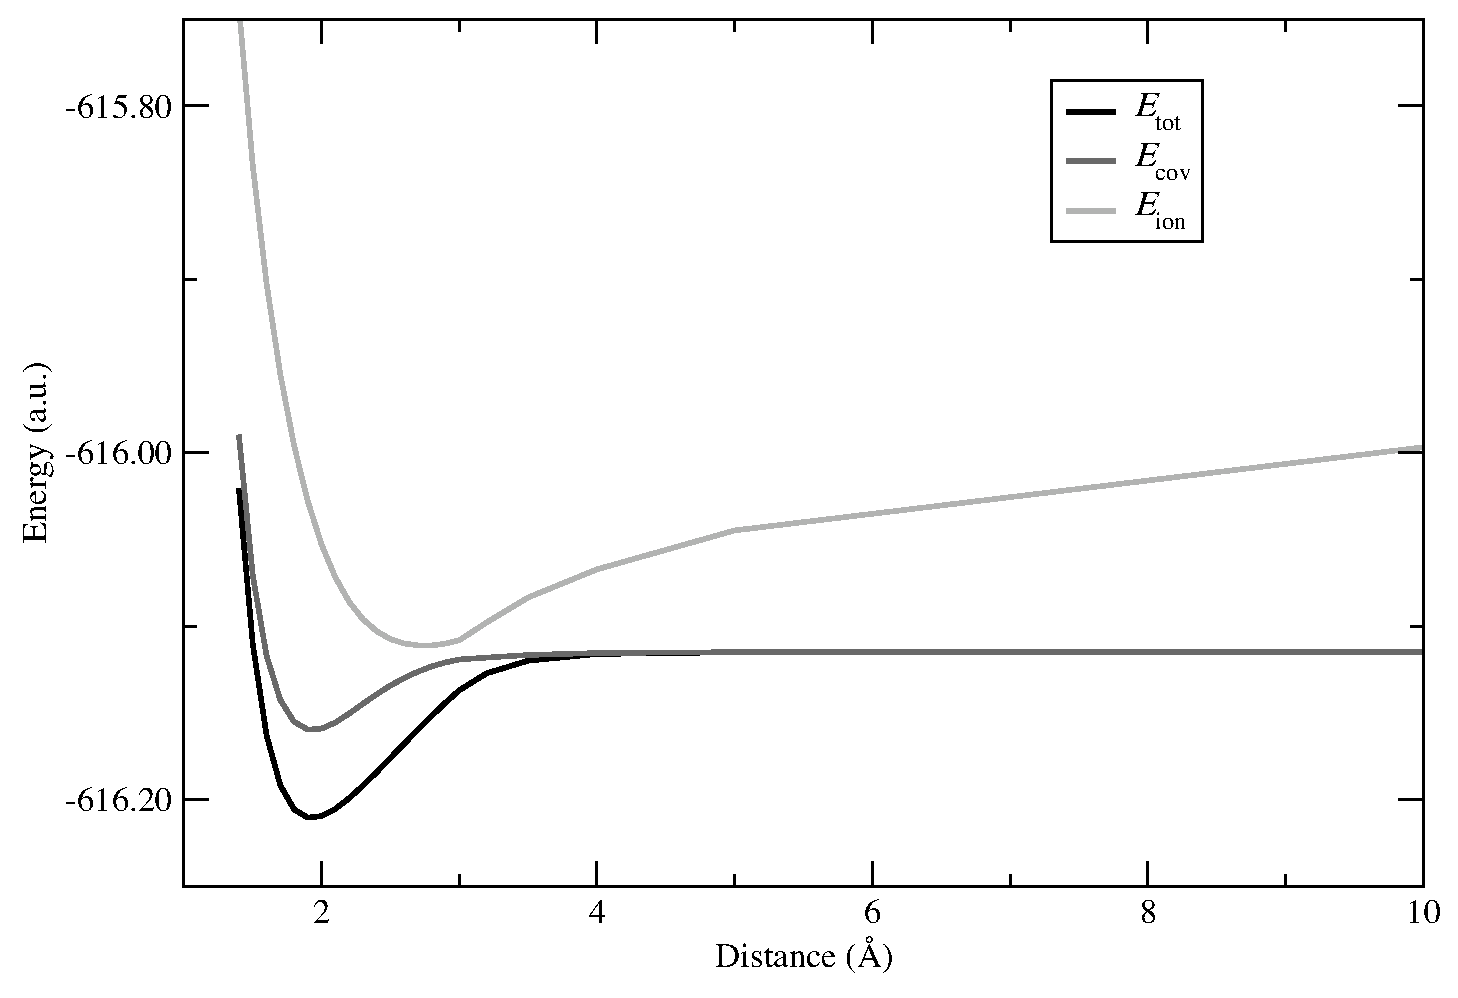
\includegraphics[scale=0.55]{dissociation/figures/c4h9cl_g.eps}
\end{center}
\caption{The dissociation curve of \textit{tert}-butylchloride (C(CH$_3$)$_3$Cl; \textbf{2}) in the gas phase. $E_\mathrm{tot}^\mathrm{gas}$ is the total VB energy. $E_\mathrm{cov}^\mathrm{gas}$ is the energy of structure \textbf{a} and $E_\mathrm{ion}^\mathrm{gas}$ is the energy of structure \textbf{b}. The minima are shown in parenthesis.}
\label{ch3.fig.c4h9cl}
\end{figure}
\begin{figure}[h]
\begin{center}
\includegraphics[scale=0.55]{dissociation/figures/sih3cl_g.eps}
\end{center}
\caption{The dissociation curve of chlorosilane (SiH$_3$Cl; \textbf{3}) in the gas phase. $E_\mathrm{tot}^\mathrm{gas}$ is the total VB energy. $E_\mathrm{cov}^\mathrm{gas}$ is the energy of structure \textbf{a} and $E_\mathrm{ion}^\mathrm{gas}$ is the energy of structure \textbf{b}. The minima are shown in parenthesis.}
\label{ch3.fig.sih3cl}
\end{figure}
\begin{figure}[h]
\begin{center}
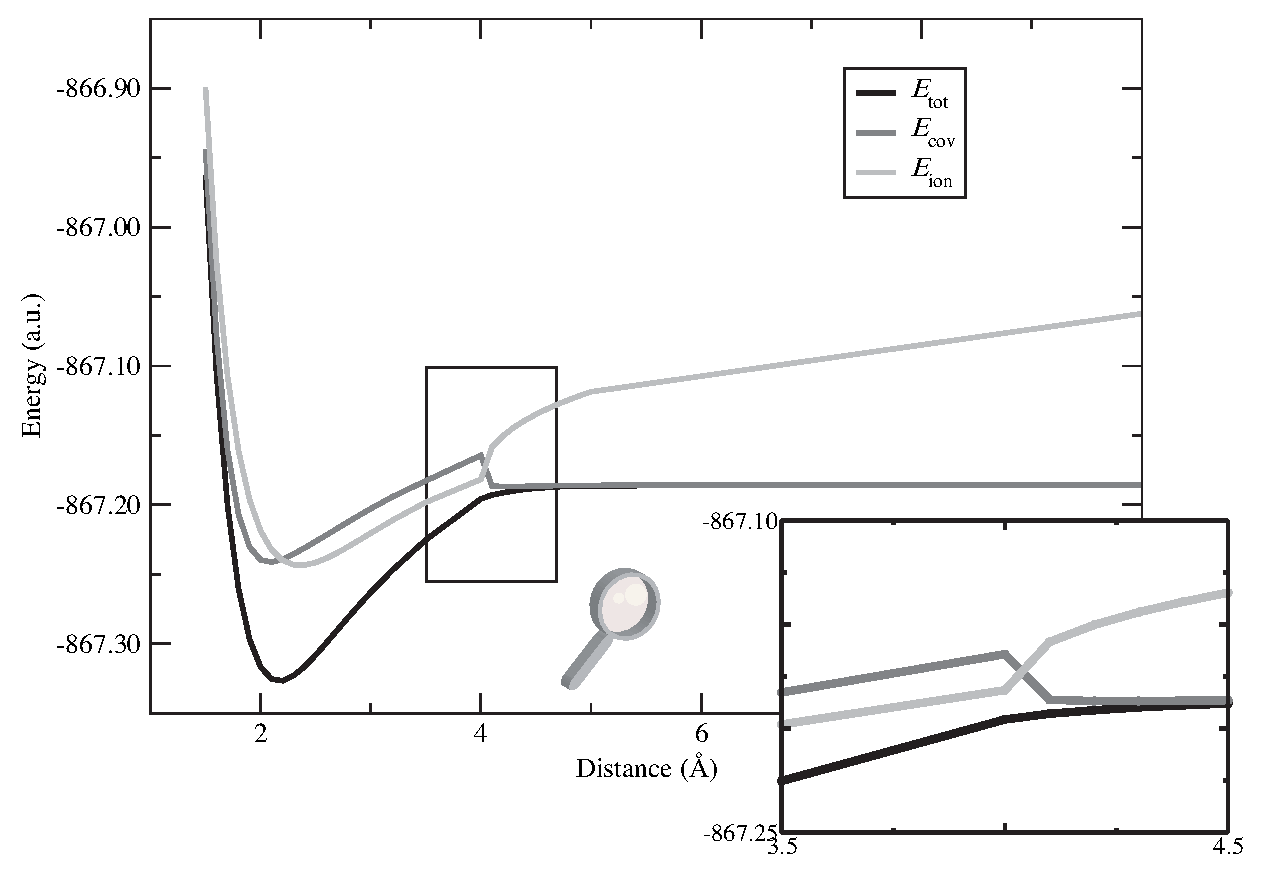
\includegraphics[scale=0.55]{dissociation/figures/c3h9sicl_g.eps}
\end{center}
\caption{The dissociation curve of trimethylsilylchloride (Si(CH$_3$)$_3$Cl; \textbf{4}) in the gas phase. $E_\mathrm{tot}^\mathrm{gas}$ is the total VB energy. $E_\mathrm{cov}^\mathrm{gas}$ is the energy of structure \textbf{a} and $E_\mathrm{ion}^\mathrm{gas}$ is the energy of structure \textbf{b}. The minima are shown in parenthesis.}
\label{ch3.fig.c3h9sicl}
\end{figure}
Chloromethane (\textbf{1}; Figure \ref{ch3.fig.ch3cl}) shows covalent bond character over the whole range. The weight of the covalent structure is 0.67 at equilibrium distance and higher for longer distances. The bond character for \textit{tert}-butylchloride (\textbf{2}; Figure \ref{ch3.fig.c4h9cl}) is also covalent, because the weight for the covalent structure is at least 0.66 over the whole range of the curve. In the chlorosilane (\textbf{3}) case (Figure \ref{ch3.fig.sih3cl}) the bonding energy is 74.6 kJ/mol higher than in the chloromethane (\textbf{1}) case (Table \ref{ch3.tab.optimal}), indicating that the Si--Cl bond is much stronger than the C--Cl bond. 

For trimethylsilylchloride (\textbf{4}; Figure \ref{ch3.fig.c3h9sicl}) the Coulombic character is more pronounced. For distances from 2.0 to 4.1 \AA\  the ionic curve ($E_\mathrm{ion}^\mathrm{gas}$) lies below the covalent curve ($E_\mathrm{cov}^\mathrm{gas}$). The weight of the ionic structure is higher than that of the covalent structure between 2.3 and 4.1 \AA, which is in line with the expectation that this bond possesses a higher ionic character. Still, the bonds in trimethylsilylchloride (\textbf{4}) and NaCl are quite different, because for the NaCl ``molecule'' the ionic and total curve almost coincide, while for \textbf{4} this is not the case, although the ionic curve lies lower in energy than the covalent curve near the equilibrium distance. At large distance this situation is reversed (compare Figure \ref{ch3.fig.nacl_c} with Figure \ref{ch3.fig.c3h9sicl}). Regarding the shape of the curve, at the crossing of the ionic and covalent curves for \textbf{4} around 2.2 \AA\ the geometry does not change drastically. Therefore, this crossing is not accompanied by any kind of discontinuity in contrast to the crossing around 4.0 \AA\ (\textit{vide infra}). At distances shorter than the Si--Cl equilibrium bond distance the negative charge cloud on the chlorine atom starts to overlap with the positive Si(CH$_3$)$_3$ fragment. This stabilizes the neutral covalent structure, which results in a lower value for $E_\mathrm{cov}^\mathrm{gas}$ than for $E_\mathrm{ion}^\mathrm{gas}$. 

Regarding the shape, the total energy ($E_\mathrm{tot}^\mathrm{gas}$) for \textbf{4} increases more gradually than for \textbf{2}, showing more Coulombic character. This is because from the equilibrium distance to the crossing, the ionic curve lies below the covalent curve, similar to the NaCl curves. In the other cases the covalent curve lies below the ionic curve over the whole range. An analysis of the Mulliken population on the chlorine and carbon/silicon atoms corroborates the Coulombic shape for \textbf{4}: the population on chlorine ($Z$=17) is 17.24 for \textbf{2} and 17.51 for \textbf{4}. While the population on carbon ($Z$=6) is 6.03 for \textbf{2}, the population on silicon ($Z$=14) for \textbf{4} is only 12.88. This suggests that the methyl groups have a slight electron donating character in \textit{tert}-butyl, while in the trimethylsilyl case they have an electron withdrawing effect. The extra Coulombic attraction results in a (much) stronger bond for \textbf{4} (371.5 kJ/mol) than for \textbf{2} (251.3 kJ/mol). 

An intriguing feature seen in Figures \ref{ch3.fig.c4h9cl} and \ref{ch3.fig.c3h9sicl} is the abrupt rise in energy of the ionic curve at around 3.0 \AA\ for \textbf{2} and around 4.0 \AA\ for \textbf{4} and the abrupt fall in energy of the covalent curve at the same points. In contrast, the total energy rises modestly with increasing bond distance at those points. To understand this behavior, one has to examine the underlying geometry of the molecules at these points. For \textbf{4}, the effect is most pronounced and will be discussed here. For \textbf{2}, the same reasoning can be applied. The reason for the crossing of the covalent and ionic curves is that the geometry for \textbf{4} at 4.0 \AA\ is completely different from that at 4.1 \AA. At 4.0 \AA\ the bond is ionic and hence the trimethylsilyl fragment is cation-like in which the silicon and the three carbon atoms are nearly coplanar after geometry optimization (Figure \ref{ch3.fig.crossing}(a)). This geometry is unfavorable for the covalent structure alone, reflected in the high energy.  In contrast, at 4.1 \AA\  the bond is covalent and the trimethylsilyl is radical-like, in which the silicon and the three carbon atoms form a tetrahedral structure (Figure \ref{ch3.fig.crossing}(b)), resulting in a lower covalent structure energy. 
\begin{figure}[hbtp]
\center
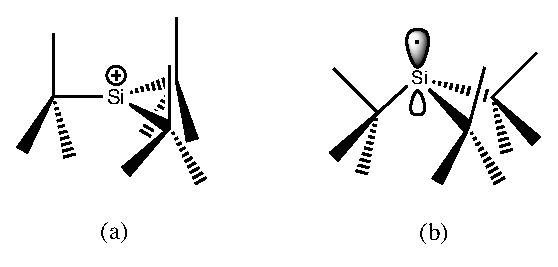
\includegraphics[scale=1.0]{dissociation/figures/crossing.eps}
\caption{The cation-like structure with coplanar silicon (M=Si), carbon (M=C)) and methyl carbon atoms (a) and the radical-like tetrahedral structure (b).}
\label{ch3.fig.crossing}
\end{figure}
Note that the total energy curve ($E_\mathrm{tot}^\mathrm{gas}$) does not show any irregularities.  The wave function changes drastically in character at this point. This compound follows the dissociation path of the ionic structure at short distances and that of the covalent structure at longer distances. 

A notable difference between the gas dissociation curve in Figure \ref{ch3.fig.c3h9sicl}  and the one presented by Su \textit{et al.} in reference \cite{psu} is that here the covalent and ionic curves cross at 4.1 \AA, while in the article by Su, the curves cross around 5.5 \AA. The reason for this is probably the difference in geometry. For the research presented here, a multideterminant wave function of the GVB type is used for the geometry optimization, while Su \textit{et al.} make use of a single determinant MP2 \cite{mp2} wave function.

A comparison of the hydrogen and methyl substituted molecules suggests that methyl substitution has an energy lowering effect on the $E_\mathrm{ion}^\mathrm{gas}$ with respect to $E_\mathrm{cov}^\mathrm{gas}$. In the silicon case (\textbf{4}), the ionic curve even lies below the covalent curve between 2.3 and 4.1 \AA.

\section{\label{ch3.sec.solv}Solvation Effects}

\subsection{Computational Methods}

In the Polarizable Continuum Model (PCM) the solvent is represented as a homogeneous medium that is characterized by its dielectric constant. No further explicit molecular interactions between the solvent molecules and the solute are taken into account. For example, hydrogen-bond formation is absent. For the research presented here, the VB module TURTLE and the PCM algorithm in GAMESS-UK were linked.

The PCM model requires a number of parameters. First of all, a dielectric constant, for which the value of water (H$_2$O, $\epsilon$=78.5) was chosen. The second parameter is the interspacing of the point charges, which was set to 30.0\degrees. The last set of parameters contains the dimensions of the spheres around the atoms. As an estimate for these the van der Waals radii \cite{bondi} were taken, scaled by 1.20 (being the average of the optimal 1.15 for ions and 1.25 for neutral atoms \cite{scaling}) resulting in 1.44 \AA\  for hydrogen, 2.16 \AA\  for carbon, 2.69 \AA\ for silicon and 2.10 \AA\ for chlorine and chloride.

For each compound two points on the potential energy curve were analyzed with VBPCM. One calculation was performed at the equilibrium distance and one at large distance (10 \AA). For the point at equilibrium distance the gas phase optimized geometries were taken. For the point at large distance the R$_3$M-fragments were optimized in two ways: as the covalent structure (a geometry optimization on the radical R$_3$M$^\bullet$-fragments) and as the ionic structure (a geometry optimization on the R$_3$M$^{+}$-fragments). Subsequently, the chlorine atoms were added to the R$_3$M-fragments at a distance of 10 \AA. 

\subsection{Results and Discussion}

In Table \ref{ch3.tab.solution} the VBPCM values are presented for the equilibrium distance ($E_\mathrm{R_{3}M-Cl}^\mathrm{solv}$) and for both neutrally and ionically optimized geometries at large distance (10 \AA), $E_\mathrm{R_{3}M^\bullet Cl^\bullet}^\mathrm{solv}$ and $E_\mathrm{R_{3}M^{+} Cl^{-}}^\mathrm{solv}$ respectively. Besides, the dissociation energy in the gas phase ($E_\mathrm{dis}^\mathrm{gas}$) and in solution ($E_\mathrm{dis}^\mathrm{solv}$) are shown in the last two columns.
\begin{table}[htp]
\center
\caption{The VBPCM energy at equilibrium distance ($E_\mathrm{R_{3}M-Cl}^\mathrm{solv}$), the VBPCM energies on the neutrally ($E_\mathrm{R_{3}M^\bullet Cl^\bullet}^\mathrm{solv}$) and ionically ($E_\mathrm{R_{3}M^{+} Cl^{-}}^\mathrm{solv}$) optimized geometries at long distance (10 \AA), and the dissociation energy ($E_\mathrm{dis}^\mathrm{solv}$), being the difference between the most stable long distance geometry (\textit{italics}) and the energy at equilibrium distance ($R_\mathrm{eq}$). The last column contains the dissociation energies from Table \ref{ch3.tab.optimal}. Energy values are in atomic units, except $E_\mathrm{dis}^\mathrm{solv}$ and $E_\mathrm{dis}^\mathrm{gas}$, which are in kJ/mol.}
\begin{tabular}{|l|c|c|c|c|c|}
\hline
\textbf{Compound} & $E_\mathrm{R_{3}M-Cl}^\mathrm{solv}$ ($E_{\mathrm{h}}$) & $E_\mathrm{R_{3}M^\bullet Cl^\bullet}^\mathrm{solv}$ ($E_{\mathrm{h}}$) & $E_\mathrm{R_{3}M^{+} Cl^{-}}^\mathrm{solv}$ ($E_{\mathrm{h}}$) & $E_\mathrm{dis}^\mathrm{solv}$&
$E_\mathrm{dis}^\mathrm{gas}$\\
\hline
CH$_3$Cl (\textbf{1})& --499.102862 & \textit{--499.000733} & --498.984663 & 268.1 & 260.9 \\
C(CH$_3$)$_3$Cl (\textbf{2})& --616.215591 & --616.116711 & \textit{--616.165131} & 132.5 & 251.3 \\
SiH$_3$Cl (\textbf{3})& --750.179837 & --750.049132 & \textit{--750.065038} &  301.4 & 335.5 \\
Si(CH$_3$)$_3$Cl (\textbf{4})& --867.333824 & --867.187477 & \textit{--867.248816} & 223.2 & 371.5 \\
\hline
\end{tabular}
\label{ch3.tab.solution}
\end{table} 

The ionic structures are more stabilized by the polar solvent than the covalent structures. At large distances the ionic structure has a lower energy ($E_\mathrm{ion}^\mathrm{solv}$) for \textbf{2}, \textbf{3} and \textbf{4} in the polar medium. This indicates that for these molecules the dissociation changes from homolytic to heterolytic with PCM in the presence of a polar solvent (here H$_2$O). For \textbf{1}, which contains the least polar bond, the ionic structure is stabilized, however, not enough to change the dissociation to heterolytic in the solvent model.

For both the methyl substituted compounds, the lowering in dissociation energy in solution compared to the gas phase is standing out, most remarkable for \textbf{2}. While in the gas phase the dissociation energy of \textbf{4} is higher than for \textbf{3}, in solution the situation is reversed. The reason for this is the stabilization of the planar structure of the \textit{tert}-butyl and \textit{tert}-silyl  (Figure \ref{ch3.fig.crossing}(a)) cations in solution compared to the umbrella shaped radical fragment in the gas phase (Figure \ref{ch3.fig.crossing}(b)).

\section{The Frozen Orbital Approximation}

Upon comparing the ionic and covalent curves for \textit{tert}-butylchloride (\textbf{2}) shown in Figure \ref{ch3.fig.c4h9cl} with those in the article by Song \textit{et al.} \cite{song}, we have noted that in the article by Song the ionic and covalent curves cross twice, while in our curves there is no crossing between the two curves. One difference between both calculations appeared to be the use of frozen orbitals for the C--H bonds by Song, while we optimized those with the other orbitals. Therefore, the impact of the freezing of orbitals will be investigated here for \textbf{2}.

\subsection{Computational Methods}

Two points on the C--Cl reaction coordinate were taken, one at equilibrium distance and one at \mbox{10 \AA}. For the point at 10 \AA, the umbrella shaped \textit{tert}-butyl fragment was used for the gas phase (Figure \ref{ch3.fig.crossing}(b)), while the planar shaped fragment was used for in solution (Figure \ref{ch3.fig.crossing}(a)). The start-up orbitals for both fragments were generated with a RHF wave function with the 6-31G* basis set. For each point two sets of RHF start-up orbitals were generated: \textbf{I}) for the neutral fragments (CH$_3$)$_3$C$^\bullet$ and Cl$^\bullet$ (homolytic dissociation) and \textbf{II}) for the ions, (CH$_3$)$_3$C$^{+}$ and Cl$^{-}$ (heterolytic dissociation). Subsequently, the orbitals on the (CH$_3$)$_3$C$^\bullet$ and (CH$_3$)$_3$C$^{+}$ fragments were localized using the Foster-Boys algorithm \cite{foster}. The localized orbitals describing the inner-shells and C--H bonds were frozen during the subsequent VB calculations, as were the core orbitals of chlorine and carbon. For the PCM solvation model the same parameters as in Section \ref{ch3.sec.solv} were used.

\subsection{\label{ch3.sec.res.freez}Results and Discussion}

The total VB energies for calculations with start-up sets \textbf{I} and \textbf{II}, together with the VB energies from Section \ref{ch3.sec.solv} ($E_\mathrm{free}$) are given in Table \ref{ch3.tab.frozen}. 
\begin{table}[htp]
\center
\caption{VB energies without frozen C--H bonds ($E_\mathrm{free}$), with frozen C--H bonds based on
start-up set \textbf{I} ($E_\mathrm{froz-\textbf{I}}$) and with frozen C--H bonds based on start-up set \textbf{II}
($E_\mathrm{froz-\textbf{II}}$) at equilibrium distance ($R_{eq}$) and at 10.0 \AA\ ($R_{10.0 \text{\AA}}$),
both in the gas phase and in solution (in $E_\mathrm{h}$). The dissociation energy in gas phase ($E_\mathrm{dis}^\mathrm{gas}$) and in solution ($E_\mathrm{dis}^\mathrm{solv}$), both in kJ/mol.}
\center
\begin{tabular}{|c|cc|cc|c|c|}
\hline
&\multicolumn{2}{c|}{$R_{eq}$}&\multicolumn{2}{c|}{$R_{10.0 \text{\AA}}$} & $E_\mathrm{dis}^\mathrm{gas}$ & $E_\mathrm{dis}^\mathrm{solv}$ \\
\textbf{Energy} & gas & solv & gas & solv &  & \\
\hline
$E_\mathrm{free}$ & {--616.210349} & {--616.215591} & {--616.114616} & {--616.165131} & 251.3 & 132.5 \\
$E_\mathrm{froz-\textbf{I}}$& {--616.208752} & {--616.213543} & {--616.114616} & {--616.132413} & 247.2 &  213.0 \\
$E_\mathrm{froz-\textbf{II}}$& {--616.186693} & {--616.194963} & {--616.080074} & {--616.164974} & 279.9 & 78.7\\
\hline
\end{tabular}
\label{ch3.tab.frozen}
\end{table}

The values on the first row of the table correspond to those presented earlier in this chapter. The energy value at 10 \AA\ in the gas phase is equal to the corresponding energy value with the freely optimized orbitals ($E_\mathrm{froz-\textbf{I}}^{R_{10.0 \text{\AA}},\mathrm{gas}}$ = $E_\mathrm{free}^{R_{10.0 \text{\AA}},\mathrm{gas}}$ = {--616.114616}). The reason is that at 10 \AA\ both fragments are so far apart that they can be considered as two separate radicals. Since the orbitals are optimized for radicals, they do not need to change much and hence, frozen or not, they are already optimal from the start. At equilibrium distance,  both fragments are closer and hence, the free C--H orbitals are adopted to the presence of the chlorine atom ($E_\mathrm{free}^{R_{eq},\mathrm{gas}}$ = {--616.210349}, opposed to $E_\mathrm{froz-\textbf{I}}^{R_{eq},\mathrm{gas}}$ = {--616.208752}). In solution, the difference at equilibrium distance is smaller than in the gas phase ($E_\mathrm{free}^{R_{eq},\mathrm{solv}}$ = {--616.215591}, compared to $E_\mathrm{froz-\textbf{I}}^{R_{eq},\mathrm{solv}}$ = {--616.213543}). At 10.0 \AA\ the difference is large, $E_\mathrm{free}^{R_{10.0 \text{\AA}},\mathrm{solv}}$ = {--616.165131}, compared to $E_\mathrm{froz-\textbf{I}}^{R_{10.0 \text{\AA}},\mathrm{solv}}$ = {--616.132413}. Since C(CH$_3$)$_3$Cl dissociates to ions in solution, the start up with frozen orbitals for radicals appears to be unfavorable. The dissociation energy in solution ($E_\mathrm{dis}^\mathrm{solv}$) goes up from 132.5 kJ/mol for free orbitals to 213.0 kJ/mol for frozen orbitals started with radicals.

The frozen orbitals for ionic fragments result in much higher energies at equilibrium, both in the gas phase as in solution, \textit{viz.} $E_\mathrm{froz-\textbf{II}}^{R_{eq},\mathrm{gas}}$ = {--616.186693} and $E_\mathrm{froz-\textbf{II}}^{R_{eq},\mathrm{solv}}$ = {--616.194963}, compared to the corresponding values for $E_\mathrm{free}$. Also the energy for the gas phase at 10 \AA\ is much higher than for free orbitals, $E_\mathrm{froz-\textbf{II}}^{R_{10.0 \text{\AA}},\mathrm{gas}}$ = {--616.080074} compared to $E_\mathrm{free}^{R_{10.0 \text{\AA}},\mathrm{gas}}$ = {--616.114616}. The only energy value for ionically optimized start up orbitals that is close to the corresponding value for free orbitals, is the one in solution at 10 \AA, $E_\mathrm{froz-\textbf{II}}^{R_{10.0 \text{\AA}},\mathrm{solv}}$ = {--616.164974} compared to $E_\mathrm{free}^{R_{10.0 \text{\AA}},\mathrm{solv}}$ = {--616.165131}. This can easily be explained. Since \textbf{2} dissociates to ions in solution, the ionic C--H start up orbitals, frozen at the RHF level, are close to the optimal ones obtained with free optimization.

This indicates that the way the frozen C--H orbitals are optimized, \textit{i.e.} for the \textit{tert}-butyl radical and the \textit{tert}-butyl cation, has a non negligible influence on the wave function and hence on the dissociation energy. Therefore, the C--H bonds are not mere spectators: they play a vital role in the dissociation process. In the next section, the interaction of the C--H bonds with the central carbon atom, linked to hyperconjugation \cite{march,mcmurry}, is investigated in more detail.
 
\subsection{Hyperconjugation}

When the C--H bond orbitals are frozen, the interactions between them and the $p$ orbital on the central carbon atom are negligible in the wave function (Figure \ref{ch3.fig.hyperconjugation}).
\begin{figure}[ht]
\center
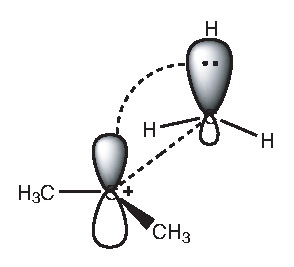
\includegraphics{dissociation/figures/hyperconj.eps}
\caption{The hyperconjugation effect: the $p$ orbital on the central carbon atom has interaction with the neighboring C--H orbital.}
\label{ch3.fig.hyperconjugation}
\end{figure}

Hyperconjugation can be included or excluded from the Valence Bond wave function by applying appropriate restrictions during orbital optimization.  Calculations on the constrained $C_\mathrm{3h}$ geometries (Figure \ref{ch3.fig.c3h}) of the \textit{tert}-butyl cation, the trimethylsilylcation, and of their radicals have been performed in which the empty/singly occupied $p$ orbital on the central carbon/silicon atom is constrained to remain strictly atomic in nature, thereby excluding the effect of hyperconjugation.
\begin{figure}[ht]
\center
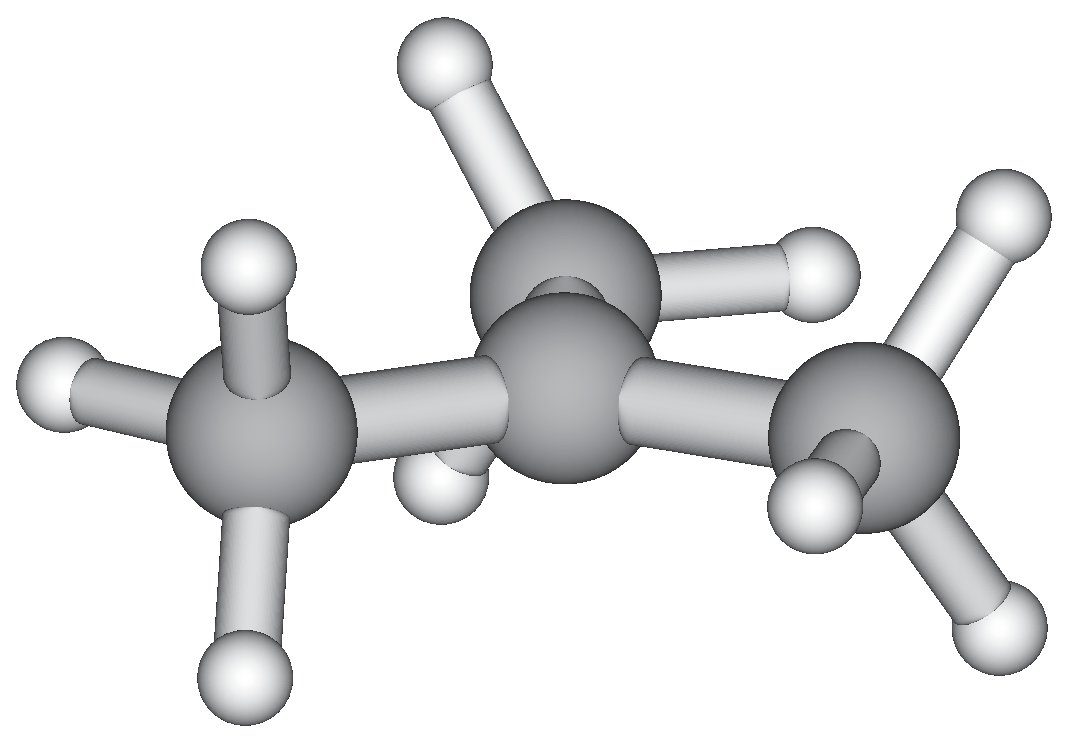
\includegraphics[scale=0.3]{dissociation/figures/c3h.eps}
\caption{Ball and stick representation of the \textit{tert}-butyl fragment in $C_\mathrm{3h}$ symmetry.}
\label{ch3.fig.c3h}
\end{figure}
A wave function that consists of several blocks of localized (orthogonal) orbitals per block is called a Block Localized Wave Function (BLW) \cite{blw}. These orbital blocks are not (necessarily) orthogonal to each other. Comparison of the energy obtained with this constrained wave function with that by an unconstrained calculation  (non localized Hartree-Fock in this case) yields an estimate of the magnitude of the stabilization by hyperconjugation for the respective cations and radicals. 

\begin{table}[htp]
\center
\caption{Energies of the cation and radical of \textit{tert}-butyl and of the cation and the radical of trimethylsilyl obtained using a constrained VB wave function with a strictly atomic $p$ orbital ($E_\mathrm{VB-res}$) in the first column. The second column shows the Hartree-Fock energies ($E_\mathrm{HF}$) and the third column contains their difference $\Delta E$ (in kJ/mol).}
\label{ch3.tab.hyp}
\begin{tabular}{|c|c|c|c|}
\hline
\textbf{Compound} & $E_\mathrm{VB-res}$ ($E_{\mathrm{h}}$) &$E_\mathrm{HF}$ ($E_{\mathrm{h}}$)& $\Delta E$ (kJ/mol)  \\
\hline
\textit{tert}-butyl cation & -156.399322 &-156.442412&113.1  \\
\textit{tert}-butyl radical & -156.630889 &-156.661317&79.9 \\
trimethylsilyl cation & -407.509449&-407.526979&46.0 \\
trimethylsilyl radical &-407.687692&-407.704949&45.3 \\
\hline
\end{tabular}
\end{table}

From a survey of the data in Table \ref{ch3.tab.hyp} it follows that the stabilization obtained for the cation and the radical by mixing of the C--H bonds with the central $p$ orbital of carbon is considerable, and substantially larger in the case of the cation than for the radical.  This  corroborates that the \textit{tert}-butyl C--H bonds of the cation differ markedly from that of the radical, as was already noted from the calculations with the different sets of frozen orbitals.  Note that for the \textit{tert}-butyl radical, the equilibrium geometry will deviate from $C_\mathrm{3h}$ symmetry, and the central $p$ orbital will rehybridize.  As a consequence of the geometric distortion and their rehybridization, the overlap between the central carbon $p$ orbital and the C--H bonds will be smaller, thus the above mentioned stabilization of 79.9 kJ/mol is an upper bound.  These calculations provide strong evidence for the large stabilizing effect that hyperconjugation exerts on the central carbon atom, and as a consequence, freezing these orbitals to describe two different reaction pathways may lead to substantial errors.  Furthermore, hyperconjugation is only important in the dissociated fragments.

For the silicon case, although a stabilization is found, it is considerably smaller than for the carbon analogue.  The trimethylsilyl cation and radical are equally stabilized.  The smaller stabilization of the trimethylsilyl fragment with respect to their carbon analogues is attributed to the more electropositive nature of silicon. Thus, hyperconjugation is less important for trimethylsilyl compounds than for the carbon analogues.

\section{Conclusions}

Both the weights and the similarity of the forms of the dissociation curves to that of H$_2$ for the C--Cl bonds of \textbf{1} and \textbf{2}, indicate that these bonds are mainly covalent.  The Si--Cl bonds are more ``Coulombic'' in nature; the shape of the dissociation curves is resembling the one of NaCl. Because neither the energy of the covalent structure nor of the ionic structure is close to the total energy, these bonds are categorized as charge-shift bonds. The abrupt rise in the ionic curve and the steep drop in the covalent curve in the dissociation curves for \textbf{2} and \textbf{4} are caused by the dramatic change in geometry, due to the change in character from ionic to covalent of the wave function. The reaction paths of the single structures in the wave function differ from that of the total three-structure wave function.

Substitution of hydrogen for methyl groups does not change the C/Si--Cl bond directly, but the methyl groups exert an effect on the dissociated fragments through hyperconjugation.  The C--H bonds participate in the reaction.  Change to a medium that mimics a polar solvent (water) stabilizes the ionic curve, and may therefore change the dissociation from homo- to heterolytic, if the resulting cation is also stabilized by its electropositiveness or hyperconjugation.
 
\section*{Acknowledgement}

Part of this research was conducted in the Laboratoire de Chimie Physique, Paris XI (France) and was funded by the European Union (a Marie Curie host fellowship) and the Netherlands Organization for Scientific Research (NWO).

\bibliography{dissociation}
\bibliographystyle{../main/achemso}

\setcounter{chapter}{3}
\setcounter{NAT@ctr}{0}
\chapter{On the Bonding of AlH$_2$, SiH and SiH$_3$ Fragments to a Cyclopentadienyl Moiety}
\footnotetext{Reproduced in part with permission from ``Trends in Cyclopentadienyl-Main-Group-Metal Bonding'', \mbox{P. H. M. Budzelaar}, \mbox{J. J. Engelberts} and \mbox{J. H. van Lenthe}, \textit{Organometallics} \textbf{2003}, \textsl{22}, 1562-1576. \copyright\ 2003 American Chemical Society.}
\label{chap_cyclopentadienyl}

\ifthenelse{\boolean{wholethesis}}{\relax}{\begin{center}\textit{Generated on \today\ at \currenttime}\end{center}}

\noindent\textbf{Abstract:} In this chapter the bonding mechanism of three main group metal hydride moieties, AlH$_2$, SiH and SiH$_3$, to a cyclopentadienyl ring are analyzed with Valence Bond wave functions. In CpAlH$_2$ and CpSiH the metal hydride groups are situated above a C-C bond ($\eta^2$), while the SiH$_3$ group in CpSiH$_3$ is attached to a single C-atom ($\sigma$) and positioned outside the ring. The VB energies and weights of the separate structures, the overlap between the orbitals and the resonance energy contributions indicate that the character of the bond between Cp and the metal hydrides is mainly covalent. For CpAlH$_2$ and CpSiH it is a combination of $\sigma$- and $\pi$-like structural contributions, while for CpSiH$_3$ it is $\sigma$-like only. Besides these covalent contributions in all cases a modest ionic structural contribution is discernible.

\clearpage

\section{Introduction}

\lettrine{\initial{T}}{}he way atoms bind together to form molecules has puzzled scientists over the past centuries. In 1916 Lewis wrote a historic paper about atoms and molecules on which much of today's chemical knowledge, including concepts as the ``covalent bond'' and the ``octet rule'', is based \cite{lewis}. A covalent bond between two atoms is formed when both atoms share one electron to form a two-electron pair. Regarding the octet rule Lewis wrote: ``The atom tends to hold an even number of electrons in the [outer] shell, and especially to hold eight electrons, which are normally arranged symmetrically at the eight corners of a cube.'' In 1927 Heitler and London merged the Lewis concept of a bond with quantum mechanics  by spin-coupling the orbitals on two hydrogen atoms, to represent a covalent bond \cite{heitler}. In some molecules bonds cannot be described by the spin-coupling of two orbitals on two atoms, because bonds are not necessarily restricted to two atoms, but can be extended over several atoms, like for example in benzene. A single covalent Kekul\'{e} structure would describe a molecular system with 3 double and 3 single C-C bonds, \textit{i.e.} 1,3,5-cyclohexatriene (see Figure \ref{ch4.fig.cyclohexatriene}, structure (\textbf{a})).
\begin{figure}[hbtp]
\center
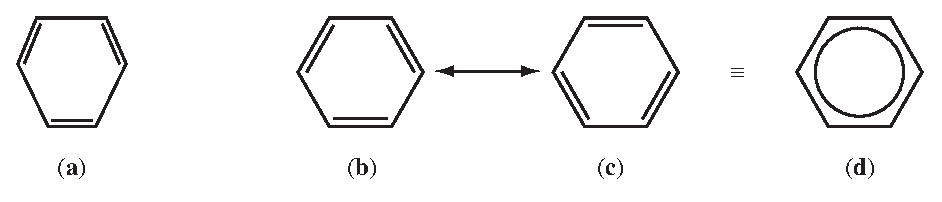
\includegraphics[scale=0.8]{cyclopentadienyl/figures/cyclohexatriene.eps}
\caption{1,3,5-cyclohexatriene (\textbf{a}), the two Kekul\'{e} structures of benzene (\textbf{b} and \textbf{c}) and the structure with delocalized $\pi$ bonds (\textbf{d}).}
\label{ch4.fig.cyclohexatriene}
\end{figure}
The two Kekul\'{e} structures together form the familiar picture with the delocalized $\pi$ electrons. On average, each carbon atom has $1\frac{1}{2}$ bond with each neighboring carbon atom. The bond order of the carbon-carbon bonds, which is a measure for the bond strength \cite{streitwieser}, is $1\frac{2}{3}$. Higher bond orders indicate stronger bonds.

Likewise, in organometallic chemistry a single bond between a metal atom and a ligand can be spread out over several ligand atoms. Bonds between metal atoms and ligands are frequently expressed in the hapticity $\eta^x$. The hapto number ($x$) is the number of ligand atoms within bonding distance of the metal \cite{powell}. This sort of bonding is commonly found in metallocenes, which have a sandwich-like structure with a metal atom clamped between two cyclopentadienyl rings. In that case transition metals form a strong, covalent, and symmetric $\eta^{5}$ bond to the cyclopentadienyl (Cp) groups.

In contrast, main group metals show a bewildering variety of bonding arrangements, from symmetric $\eta^{5}$ via various slipped $\eta^{x}$ structures all the way to pure $\sigma$, or $\eta^{1}$, bonding. In addition $\eta^{x}$ ($x>1$) structures may occur in various bridging modes. There is no single preferred structural type (for a review see \cite{jutzi}). In Figure \ref{ch4.fig.bondarr} the different idealized arrangements are shown. In the $\eta^2$ arrangement the metal atom is above the middle of a C-C bond and bonded to both carbon atoms.
\begin{figure}[ht]
\center
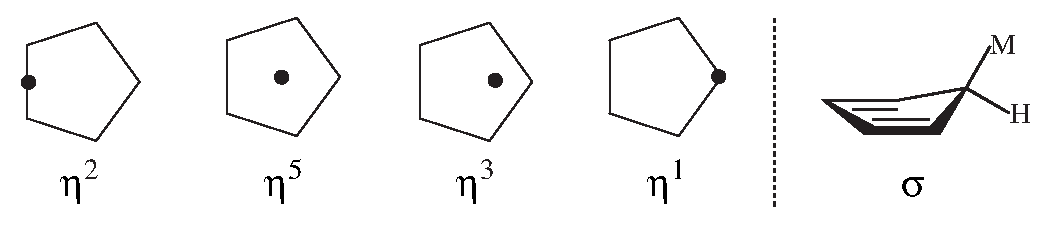
\includegraphics[scale=0.8]{cyclopentadienyl/figures/bondarrangements.eps}
\caption{Idealized representations of Cp-metal bonding arrangements. From left to right $\eta^2$, $\eta^5$, $\eta^3$ and $\eta^1$ hapticities and the $\sigma$ bonding arrangement.}
\label{ch4.fig.bondarr}
\end{figure}
The metal atom is exactly above the middle of the ring in the $\eta^5$ arrangement, having a bond with every carbon. In the $\eta^3$ and $\eta^1$ arrangements the metal atom is located almost at the same location, however, in the $\eta^1$ arrangement the metal atom is exactly positioned above one carbon atom, while in the $\eta^3$ arrangement it is positioned above three carbons. In the representation on the utmost right the metal atom is attached to the cyclopentadienyl ring via a $\sigma$ bond. 

In the transition metal series, the few exceptions to the $\eta^{5}$ bonded situation are easily explained on the basis of the electron-counting rule \cite{shriver}.
% Hoofdstuk 7 met oa "18-electron rule": het anorganische equivalent voor de octet regel van de organici.
For main group metals, no such uniform rule seems to exist. This is illustrated by the series of dicyclopentadienyl derivatives Cp$_2$M$^{+}$ of the group 13 metals B, Al, Ga, In and Tl \cite{macdonald}. These complexes show a curious alternation of structural types. Cp$_2$B$^{+}$ strongly prefers a $\eta^{5}$:$\eta^{1}$ structure. Cp$_2$Al$^{+}$ has a $\eta^{5}$:$\eta^{5}$ structure, Cp$_2$Ga$^{+}$ and Cp$_2$In$^{+}$ both have a $\eta^{5}$:$\eta^{1}$ structure and Cp$_2$Tl$^{+}$ has a $\eta^{1}$:$\eta^{1}$ structure \cite{budzelaar}. Several theoretical studies have already been devoted to these half-sandwich and sandwich complexes \cite{kwon}. Ray\'{o}n and Frenking have analyzed the bonding between main group metals (M$^{n+}$) and cyclopentadienyl anion groups ((Cp$^{-}$)$_n$; $n$=1,2) in terms of electrostatic and orbital contributions \cite{rayon}. They concluded that, except for boron, electrostatic interactions dominate the interaction energy and are more important than in the transition metal series.

In this chapter, bonds of main group metal hydrides to a single cyclopentadienyl ring (half-sandwich complexes) will be examined. This type of molecules are of interest in the increasing effort to fabricate new molecular hydrogen storage materials, as is analyzed for aluminum in reference \cite{himmel}. Also, the metal and carbon acidity of group II main group metals have recently been studied with DFT \cite{hurtado}. CpBeH behaves as a carbon acid (deprotonation occurs on the Cp-ring), whereas CpMgH and CpCaH behave as metal acids (deprotonation occurs on the metal atom). Furthermore, the bond between the ring and the metal can be considered as covalent for CpBeH, whereas it can be considered as ionic between C$_5$H$_5^{-}$ and MH$^{+}$ for CpMgH and CpCaH (for more details the reader is referred to reference \cite{hurtado}). In this chapter, half-sandwich complexes for aluminum and silicon are studied in terms of Lewis structures with Valence Bond (VB) wave functions. These VB wave functions contain multiple structures that describe the covalent and ionic bonding between the Cp-ring and the metal hydride moiety. From the contribution of each of these structures and their relative energies, the bond type can be derived. A higher contribution in combination with a lower relative structure energy is an indication for the bond character. With this information at hand, a rationalization of the preferred hapticity can be given. 

To analyze this type of bond the first two main group metals with valence electrons in the $p$ orbitals, \textit{i.e.} aluminum and silicon, are selected. To keep the molecules as simple as possible, the metal atoms have been substituted with simple hydrogen atoms. In total, the three neutral metal hydrides will be examined: AlH$_2$, SiH and SiH$_3$. A literature study revealed that no experimental data on these molecules exist.

\section{Computational Methods}

\subsection{\label{ch4.sec.geom}Geometries and Slippage Curves}

To obtain the most favorable position of the metal atom M above the Cp ring in CpAlH$_2$, CpSiH and CpSiH$_3$ the metal hydride moiety is dragged over the ring (the $\eta^2$ geometry and the direction of the slippage are shown in Figure \ref{ch4.fig.slip}).
\begin{figure}[hbtp]
\center
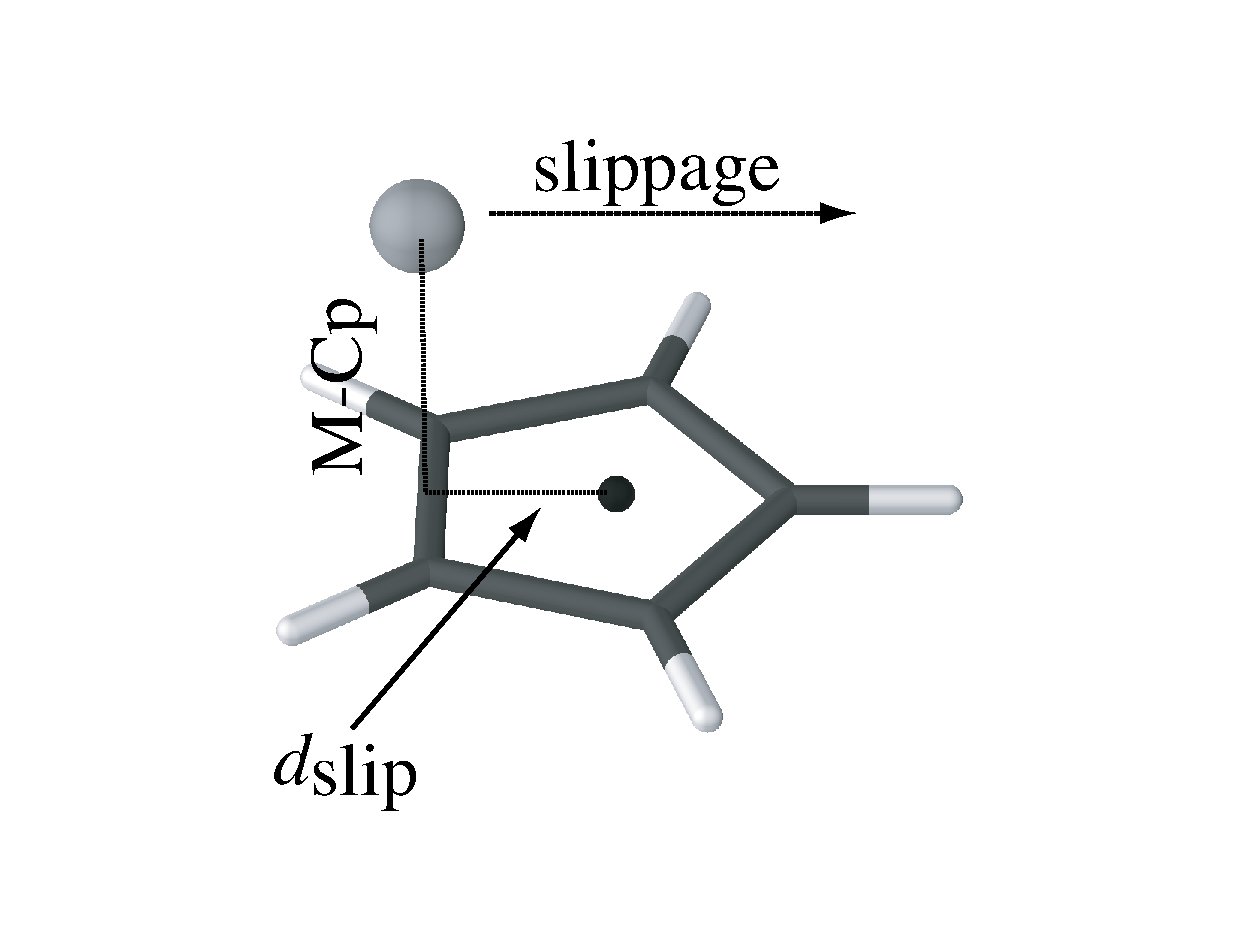
\includegraphics[scale=0.3]{cyclopentadienyl/figures/verloop.eps}
\caption{The metal hydride moiety (sphere) is dragged along a straight line over the ring from above a C-C bond ($\eta^2$; shown here) to the $\sigma$ position outside the ring via the $\eta^5$, $\eta^3$ and $\eta^1$ positions (see Figure \ref{ch4.fig.bondarr}).  $d_\mathrm{slip}$ is the distance of the projection of the metal atom M on the ring to the center of mass (black dot). M--Cp is the distance of the metal atom to the ring.}
\label{ch4.fig.slip}
\end{figure}
At fixed $d_\mathrm{slip}$ intervals of 0.3~\AA\  the geometry is optimized at the B3LYP level \cite{b3,lyp} using GAMESS-UK \cite{gamess} with the \mbox{6-31G*} basis set, maintaining the $C_\mathrm{s}$ symmetry (mirror plane on the lines M-Cp and $d_\mathrm{slip}$). Except for $d_\mathrm{slip}$, all parameters, including M-Cp are optimized. The energy for these geometries are plotted against the $d_\mathrm{slip}$ values (Section \ref{ch4.sec.slippage}). For the points nearest to the minima in the slippage curves, also the $d_\mathrm{slip}$ parameter is relaxed, which results in $C_\mathrm{s}$ constrained minima.

\subsection{Valence Bond Calculations}

On each of these $C_\mathrm{s}$ constrained slippage curve minima (two per compound) a Valence Bond (VB) calculation is performed. Hereto a VB wave function ($\Psi$) is constructed as the superposition of covalent and ionic VB structures ($\Phi_i$):
\begin{equation}
\Psi = \sum_{i} c_{i}\Phi{_i}.
\label{ch4.eq.psi}
\end{equation}
Through variational optimization, the coefficients ($c$) of these separate VB structures are obtained.
Weights for each structure, which indicate its importance in the wave function, are calculated from the coefficients ($c$) and the overlap between the structures ($S$) with \cite{coulson}:
\begin{equation}
W_{j}=\sum_{i} c_{i}c_{j}S_{ij}.
\label{ch4.eq.weight}
\end{equation}

To investigate the bond between the metal atom and the ring, the VB structures are constructed of two fragments, a metal hydride and a cyclopentadienyl fragment.  Between these two fragments several covalent and ionic bonding arrangements can be defined.

The $\pi$ system of the Cp-fragment contains the molecular orbitals shown in Figure \ref{ch4.fig.cporbs}.
\begin{figure}[htbp]
\center
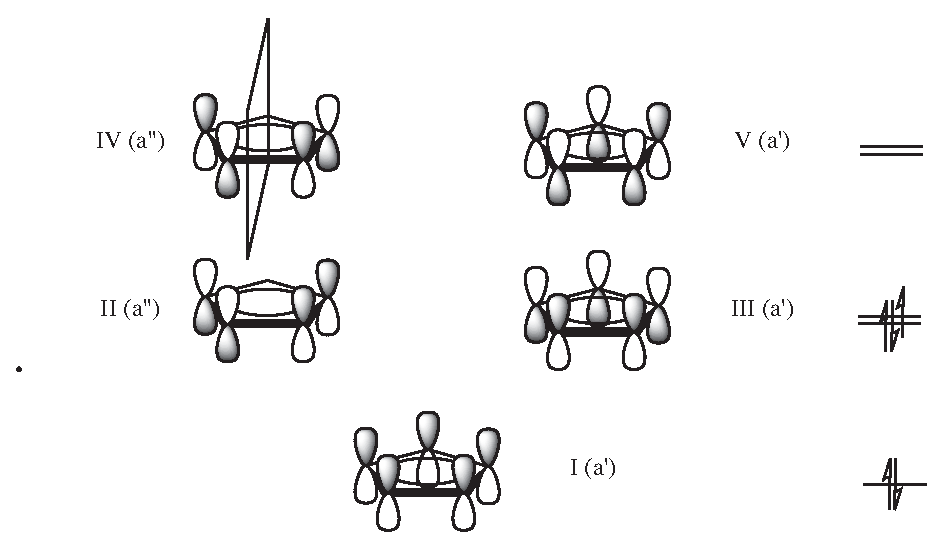
\includegraphics[scale=0.7]{cyclopentadienyl/figures/cp-orbitals.eps}
\caption{The five $\pi$ orbitals of a cyclopentadienyl radical in $C_\mathrm{s}$ symmetry (see mirror plane in orbital IV). Please note that the rings are rotated by 90\degrees\ compared to the model in Figure \ref{ch4.fig.slip}}.
\label{ch4.fig.cporbs}
\end{figure}
Since orbitals II and III are (nearly) degenerate, two electron arrangements are taken into account: in the first arrangement orbitals I and II are doubly occupied, while orbital III (a\textquotesingle) is singly occupied. In the second arrangement orbitals I and III are doubly occupied, while orbital II (a\textquotesingle\textquotesingle) is singly occupied. 

For all metal hydride fragments the most favorable spin state has to be determined. For SiH$^\bullet$, the quartet has an energy of \mbox{--289.920072} Hartree, while the doublet has an energy of \mbox{--289.988133} Hartree (for more details see \cite{kalemos}). At the B3LYP/6-31G* level of theory, CpSiH has a singlet ground state ($E_\mathrm{s}$=\mbox{--483.551896} and $E_\mathrm{t}$=\mbox{--483.460282} Hartree). This means that all metal hydride fragments favor a doublet spin state. For AlH$_2^\bullet$ and SiH$^\bullet$ there are two possible electron arrangements, one in which an a\textquotesingle\ $sp^2$-like hybridized orbital is singly occupied and one in which the a\textquotesingle\textquotesingle\ $p$ orbital is singly occupied. For SiH$_3^\bullet$ there is only one state: one with an a\textquotesingle\ $sp^3$ hybridized orbital. 

Two covalent bonds can thus be created by spin-coupling either the singly occupied a\textquotesingle\ $sp^2$-like orbitals or the singly occupied a\textquotesingle\textquotesingle\ $p$-like orbitals on both fragments. Spin-coupling the a\textquotesingle\ orbitals results in the bonding arrangement shown in Figure \ref{ch4.fig.sigma}.
\begin{figure}[htbp]
\center
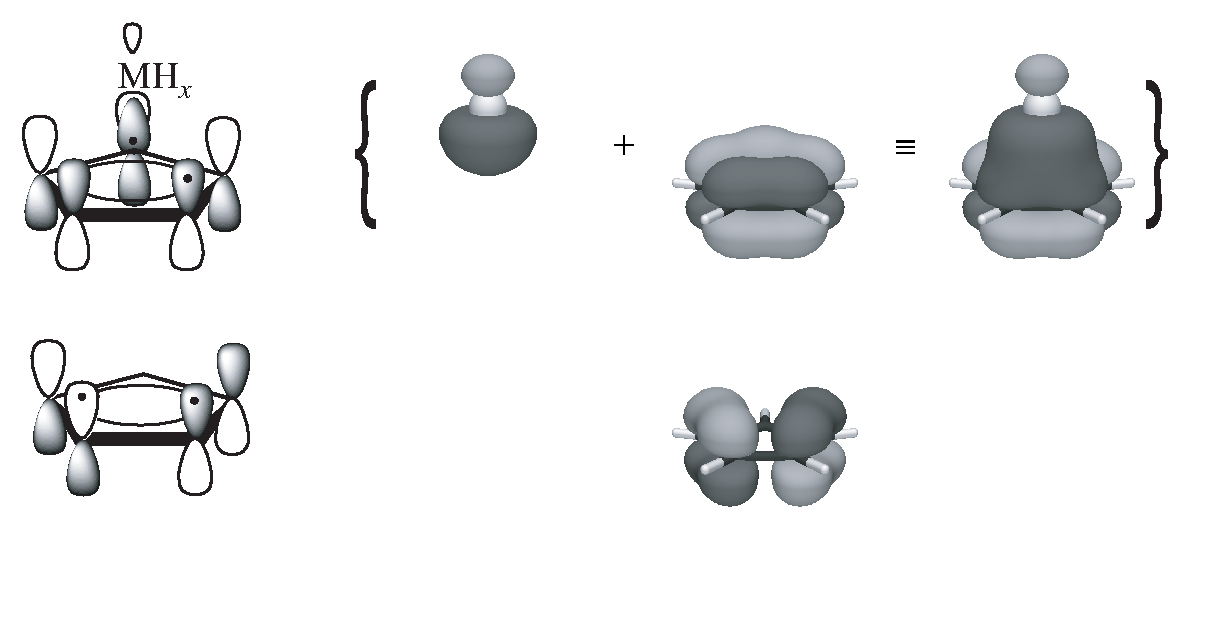
\includegraphics[scale=0.45]{cyclopentadienyl/figures/sigma.eps}
\caption{Schematic representation of the $\sigma$-like bond structure formed by coupling of the singly occupied a\textquotesingle\ orbitals (top). The a\textquotesingle\textquotesingle\ orbital on the Cp-ring is doubly occupied (bottom). Note that the MH$_x$ group is represented as a single sphere, with an $sp^2$-like hybrid orbital.}
\label{ch4.fig.sigma}
\end{figure}
This covalent bonding description will be referred to as a $\sigma$-like bond.

The other bonding arrangement is created by spin-coupling the singly occupied a\textquotesingle\textquotesingle\ orbitals on both fragments, \textit{i.e.} the $p$ orbital on the metal hydrides AlH$_{2}^\bullet$ and SiH$^\bullet$ and orbital II on the Cp-ring (Figure \ref{ch4.fig.pi}).
\begin{figure}[htbp]
\center
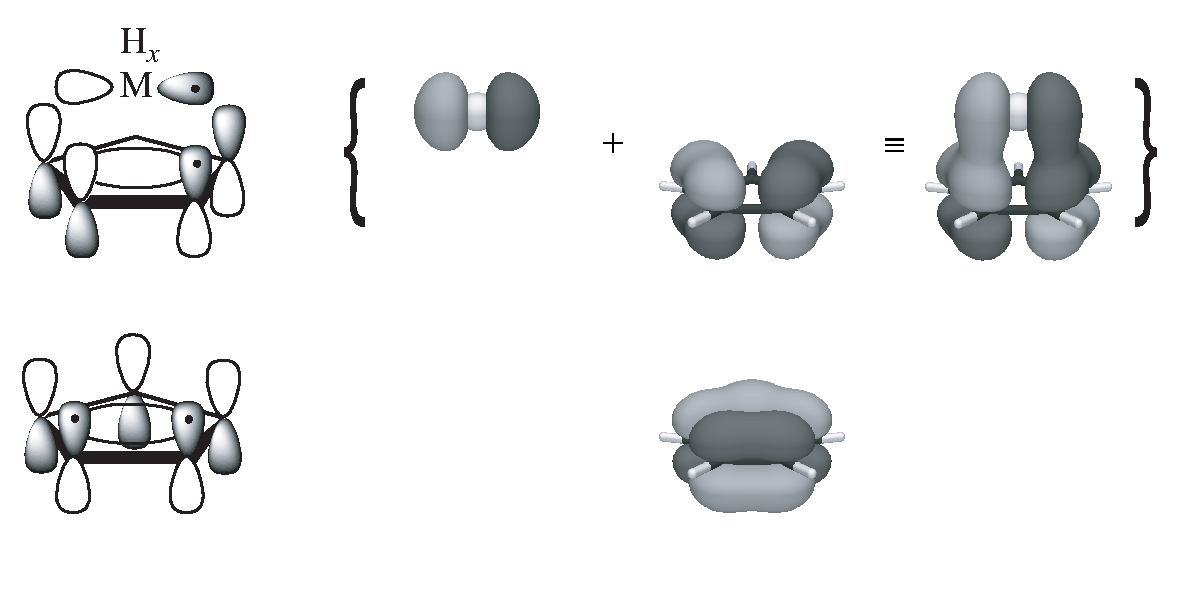
\includegraphics[scale=0.45]{cyclopentadienyl/figures/pi.eps}
\caption{Schematic representation of the $\pi$-like bond structure formed by coupling of the singly occupied a\textquotesingle\textquotesingle\ orbitals. The a\textquotesingle\ orbital on the Cp-ring is doubly occupied (bottom). Note that the MH$_x$ group is represented as a single sphere, with a p-like orbital.}
\label{ch4.fig.pi}
\end{figure}
This second covalent bonding arrangement will be referred to as $\pi$-like bond. Note that the SiH$_{3}^\bullet$ fragment does not possess a suitable a\textquotesingle\textquotesingle\ orbital for bonding due to its $sp^3$ hybridization. Therefore, for CpSiH$_3$ only one covalent structure is available.

The other VB structure used for this investigation is ionic in nature, in which the Cp-ring is negatively charged and the metal hydride moiety is positively charged (Figure \ref{ch4.fig.ionic}).
\begin{figure}[htbp]
\center
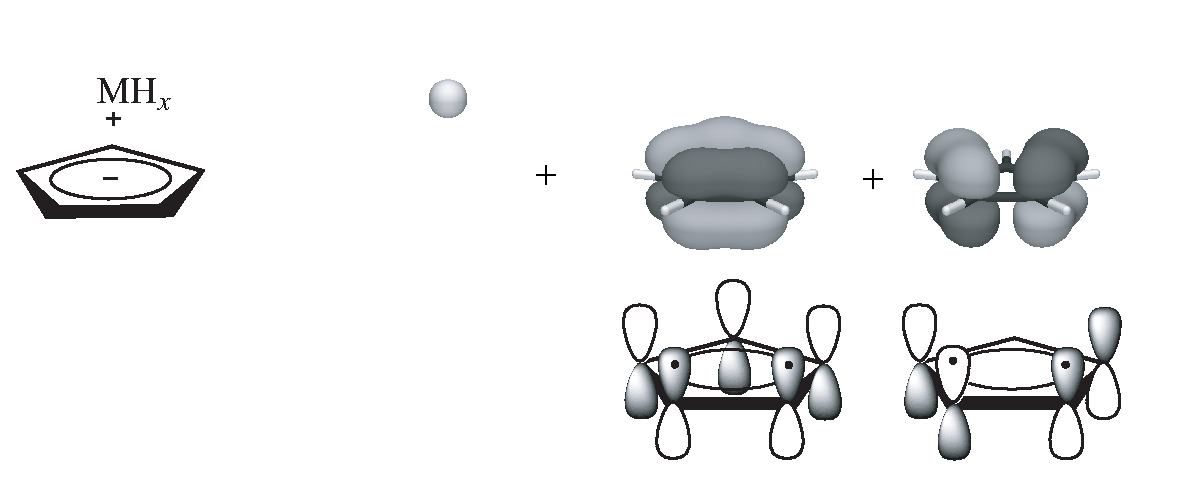
\includegraphics[scale=0.45]{cyclopentadienyl/figures/ionic.eps}
\caption{Schematic representation of the ionic structure formed by doubly occupying both the a\textquotesingle\ and a\textquotesingle\textquotesingle\ orbitals on the Cp ring. Note that the MH$_x$ group is represented as a single sphere, which is positively charged.}
\label{ch4.fig.ionic}
\end{figure}
In this situation the Cp-ring contains 6 $\pi$ electrons and is considered aromatic (H\"{u}ckel's rule, $4n+2$ $\pi$ electrons \cite{streitwieser}).

Some initial VB test calculations on another possible ionic structure in which the ring is positively charged (cyclopentadienyl cation; $4n$ $\pi$ electrons, $n$=1; anti-aromatic) and the MH$_x$ group is negatively charged (MH${_x}{^-}$) showed that the VB energy of this structure is considerably higher (\textit{ca.} 0.4 Hartree, or 1050.2 kJ/mol) than the energies of the other three structures. Therefore, this second type of ionic structure is not included in the subsequent calculations.

For each of the structures described before (Figures \ref{ch4.fig.sigma}-\ref{ch4.fig.ionic}) a separate wave function is constructed, which is separately optimized using the Valence Bond Self-Consistent Field (VBSCF \cite{vbscf1,vbscf2}) method. Orbitals on the separate fragments are kept strictly localized: orbitals on the cyclopentadienyl fragment are not allowed to mix with orbitals on the metal hydride moiety and \textit{vice versa}.

The VB calculations were carried out using the \mbox{TURTLE} program \cite{turtle} as incorporated in the GAMESS-UK package \cite{gamess}. In these studies, the \mbox{6-31G} basis was used for the carbon and hydrogen atoms, while for the main group metal atoms the 6-31G* basis was used. 

Start-up orbitals for the VB structures were created in the following way: 1. For each fragment an RHF calculation was performed. The RHF orbitals for the C-H bonds, the C-C $\sigma$-bonds and the M-H bonds were Foster-Boys localized \cite{foster}. 2. For each VB structure the appropriate fragment orbitals (Figures \ref{ch4.fig.sigma}-\ref{ch4.fig.ionic}) were combined and reoptimized in a single structure VBSCF calculation in which the innershell, the C-H bond and the M-H bond orbitals were kept frozen; 3. The final VB wave function was constructed by the combination of the VBSCF orbitals from the separate single structure calculations. The orbitals were reoptimized in which the innershell, the C-H bond and the M-H bond orbitals were still kept frozen. This type of wave function, in which each structure has its own set of orbitals, is called a Breathing Orbitals Valence Bond (BOVB \cite{bovb1,bovb2}) wave function. 
%Foster-Boys localisaties zijn geconvergeerd (outputs gecheckt op 5-1-2015).

Following this procedure  for CpAlH$_2$ and CpSiH a three VB structure wave function was obtained (the $\sigma$-like structure (Figure \ref{ch4.fig.sigma}), the $\pi$-like structure (Figure \ref{ch4.fig.pi}) and the ionic structure (Figure \ref{ch4.fig.ionic})). For CpSiH$_3$ a combined wave function of only two structures was used: the $\sigma$-like and the ionic structure.

The contributions of the different structures to the wave function were compared by investigating their weights (see equation \ref{ch4.eq.weight}), the relative energies and the resonance energy ($E_\mathrm{res}$), which is defined as the energy difference between the most stable single structure and the total energy ($E_\mathrm{tot}$) \cite{pauling}. The resonance energy of CpAlH$_2$ and CpSiH can be decomposed in contributions from ionic $\leftrightarrow$ $\sigma$ resonance, ionic $\leftrightarrow$ $\pi$ resonance and $\sigma$ $\leftrightarrow$ $\pi$ resonance by transforming the Hamiltonian matrix ($\mathbf{H}$) to a L\"owdin-orthogonalized \cite{lowdin} structure basis \cite{havenith}. The total VB energy ($E_\mathrm{VB}  = \left < \sum_{i} c_{i}\Phi{_i} | H | \sum_{j} c_{j}\Phi{_j} \right >$) can then be written as:
\begin{equation}
E_\mathrm{VB} = \sum_{i}\sum_{j}c^\prime_{i}c^\prime_{j}H_{ij}^{\bot}=\sum_{i}c^\prime_{i}c^\prime_{i}H_{ii}^{\bot}+\sum_{i}\sum_{j>i}2c^\prime_{i}c^\prime_{j}H_{ij}^{\bot}=\sum_{i}\epsilon_{i}+\sum_{i}\sum_{j>i}\epsilon_{ij},
\label{ch4.eq.energ}
\end{equation}
in which $H_{ij}^{\bot}$ is the L\"owdin-orthogonalized Hamiltonian matrix and the $c^\prime$'s are the structure coefficients in the orthogonalized basis. The energy values ($\epsilon$) are the diagonal elements ($\epsilon_{i}$), which represent the energy contributions of the orthogonalized structures themselves. The off-diagonal elements  ($\epsilon_{ij}$) are the weighted interaction energies between the structures. The sum of the off-diagonal elements is another measure of the total resonance energy ($E^{m}_{res}$), namely with respect to the weighted mean value of the energy of all structures \cite{havenith}.

\section{Results and Discussion}

\subsection{\label{ch4.sec.slippage}Geometry Optimization and Slippage Curves}

In Figures \ref{ch4.fig.slip_cpalh2}, \ref{ch4.fig.slip_cpsih} and \ref{ch4.fig.slip_cpsih3} the slippage curves obtained for CpAlH$_2$, CpSiH and CpSiH$_3$ are shown. The energy relative to the most favorable geometry is plotted as a function of  the slippage ($d_\mathrm{slip}$), which is the distance between the center of mass of the ring and the  perpendicular projection of the metal atom on the Cp-ring.
\begin{figure}[hbtp]
\center
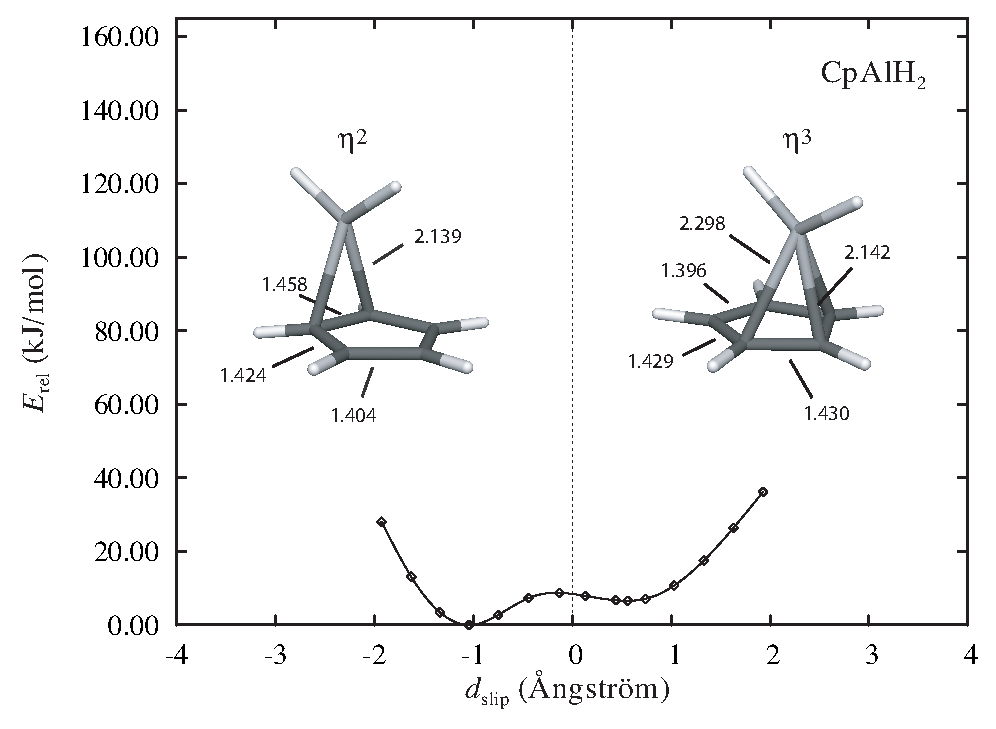
\includegraphics[scale=0.80]{cyclopentadienyl/figures/cpalh2.eps}
\caption{Slippage curve for CpAlH$_2$. The energy difference between the least favorable and the most favorable geometry (+6.7 kJ/mol) is shown. For the two minima ($\eta^2$ and $\eta^3$) the corresponding geometries with bonding distances are shown.}
\label{ch4.fig.slip_cpalh2}
\end{figure}
\begin{figure}[htbp]
\center
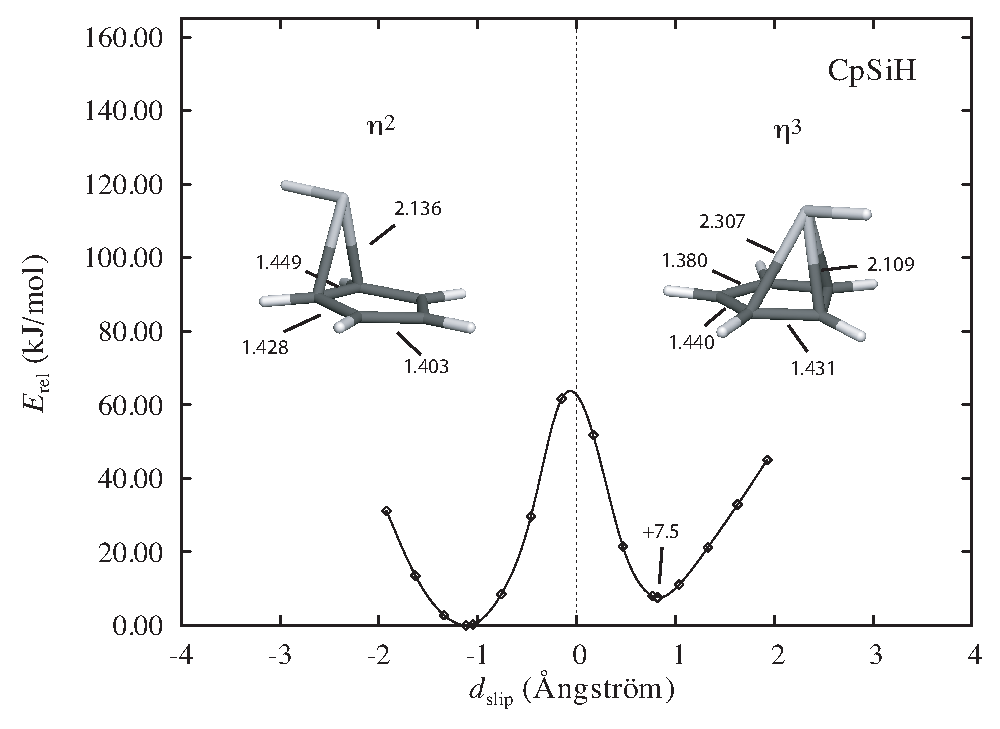
\includegraphics[scale=0.80]{cyclopentadienyl/figures/cpsih.eps}
\caption{Slippage curves for CpSiH. The energy difference between the least favorable and the most favorable geometry (+7.5 kJ/mol) is shown. For the two minima ($\eta^2$ and $\eta^3$) the corresponding geometries with bonding distances are shown.}
\label{ch4.fig.slip_cpsih}
\end{figure}
\begin{figure}[hbtp]
\center
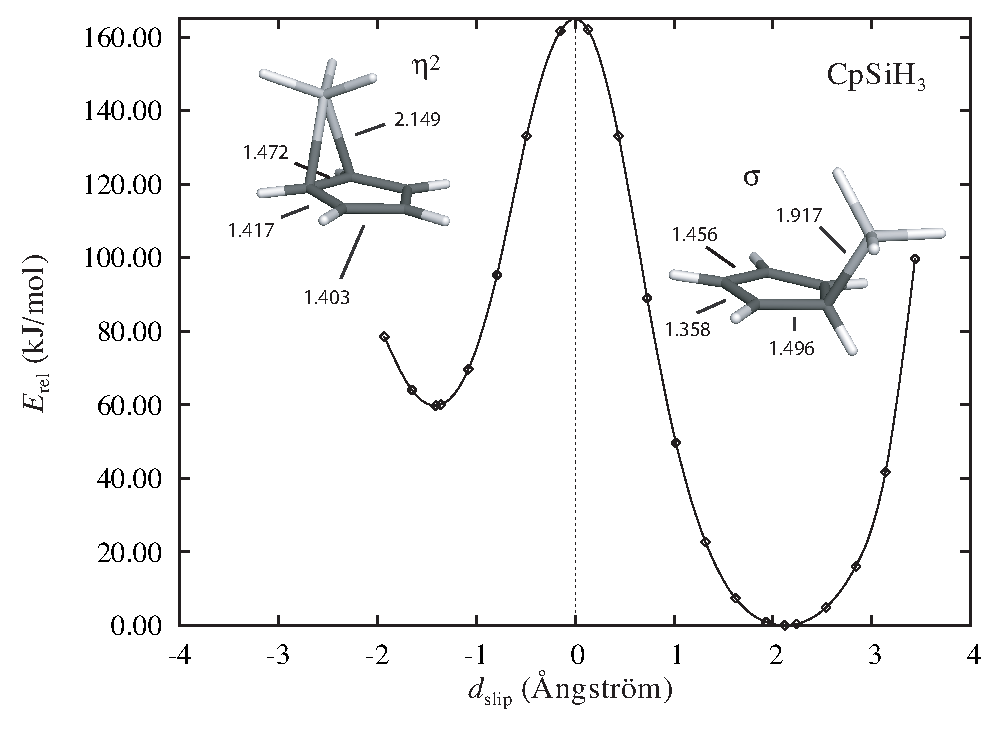
\includegraphics[scale=0.80]{cyclopentadienyl/figures/cpsih3.eps}
\caption{Slippage curves for CpSiH$_3$. The energy difference between the least favorable and the most favorable geometry (+59.8 kJ/mol) is shown. For the two minima ($\eta^2$ and $\sigma$) the corresponding geometries with bonding distances are shown.}
\label{ch4.fig.slip_cpsih3}
\end{figure}
At the B3LYP/6-31G* level of theory two stationary points are found for each molecule. Hessian calculations show that the $\eta^2$ geometries of CpAlH$_2$ and CpSiH and the $\sigma$ geometry of CpSiH$_3$ correspond to real minima. The $\eta^3$ geometries of CpAlH$_2$ and CpSiH and the $\eta^2$ geometry of CpSiH$_3$, which all possess only one imaginary frequency, are transition states connecting two equivalent $\eta^2$ geometries on neighboring carbon-carbon bonds in the case of CpAlH$_2$ and CpSiH and two equivalent $\sigma$ geometries on neighboring carbon atoms in the case of CpSiH$_3$. Hessian calculations for the maxima found at the $\eta^5$ positions show two imaginary frequencies for each molecule and are therefore higher order transition states. This means that the slippage curves are no reaction paths and that the metal hydride fragment migrates between the minima ($\eta^2$ for CpAlH$_2$ and CpSiH; $\sigma$ for CpSiH$_3$) along the perimeter of the ring via the ($\eta^3$ for CpAlH$_2$ and CpSiH and $\eta^2$ for CpSiH$_3$) transition states.

Table \ref{ch4.tab.slip} summarizes data obtained from the slippage curves.
\begin{table}[htbp]
\center
\caption{The potential energy with respect to the most favorable geometry, M--Cp, $d_\mathrm{slip}$, the total B3LYP/6-31G* energy and the imaginary frequency (if present) for the two $C_\mathrm{s}$ minima of CpAlH$_2$, CpSiH and CpSiH$_3$.}
\begin{tabular}{|c|c|c|c|c|c|}
\hline
\textbf{Molecule}&
$E_\mathrm{rel}$&
M--Cp&
$d_\mathrm{slip}$&Total B3LYP/6-31G* energy&
$\tilde{\nu}$\\
&(kJ/mol)&(\AA)&(\AA)&(Hartree)& (cm$^{-1}$)\\
\hline
CpAlH$_2$ ($\eta^{2}$) & (0)  & 2.01 & 1.04 & -437.143483 & -\\
CpAlH$_2$ ($\eta^{3}$) & 6.7  & 2.01 & 0.56 & -437.140975 & 93.5$i$ \\
CpSiH ($\eta^{2}$) & (0)  & 2.00 & 1.12 & -483.551896 & -\\
CpSiH ($\eta^{3}$) & 7.5  & 2.00 & 0.82 & -483.548987 & 108.3$i$ \\
CpSiH$_3$ ($\sigma$) & (0)  & 1.74 & 2.12 & -484.793270 & - \\
CpSiH$_3$ ($\eta^{2}$) & 59.8 & 1.97 & 1.41 & -484.770466 & 380.2$i$ \\
\hline
\end{tabular}
\label{ch4.tab.slip}
\end{table}
Both CpSiH and CpAlH$_2$ show a preference of the $\eta^{2}$ geometry over the $\eta^{3}$ geometry. For the transition states, the aluminum atom in CpAlH$_2$ lies closer to the center of mass (C$_m$) than the silicon atom of CpSiH, 0.56 \AA\ \textit{vs} 0.82 \AA\ respectively. The bonding distances to the nearest carbon atoms, however, do not differ much, 2.298 \AA\ and 2.142 \AA\ for CpAlH$_2$ \textit{vs} 2.307 \AA\ and 2.109 \AA\ for CpSiH. Therefore, both geometries are denoted as $\eta^{3}$.

While the C-C bonds in CpAlH$_2$ and CpSiH (and CpSiH$_3$ in the $\eta^2$ geometry) differ slightly (Figures \ref{ch4.fig.slip_cpalh2} and \ref{ch4.fig.slip_cpsih}), the C-C bonds in the $\sigma$ geometry in CpSiH$_3$ differ more than a tenth of an \AA ngstr\"{o}m (Figure \ref{ch4.fig.slip_cpsih3}). The bond length equalization in the former two cases is indicative for aromatic behavior for the Cp-ring: from a geometric point of view, the Cp-rings in CpAlH$_2$ and CpSiH are aromatic, while the Cp-ring in CpSiH$_3$ ($\sigma$ geometry) is not. This is also indicated by the fact that the carbon to which the silicon atom is bonded is $sp^3$ hybridized, which is reflected in the geometric position of the metal atom \textit{outside} the ring ($d_\mathrm{slip}$=2.12 \AA). 

Ray\'on and Frenking have also theoretically analyzed main group metallocenes \cite{rayon}. They found that silicon and aluminum prefer the $\eta^5$ geometry, \textit{i.e.} the metals hover above the center of the Cp-ring. The metal hydride atoms, used in the research described here, have a preference for the $\eta^2$ and $\eta^3$ geometry. The $\eta^5$ geometry corresponds to a second order saddle point (Figures \ref{ch4.fig.slip_cpalh2} - \ref{ch4.fig.slip_cpsih3}). The reason is that the bonds between the Cp-rings and the metal hydride moieties are mainly covalent (see the next section), while Ray\'on and Frenking conclude that the bond between the metal atom and the two Cp-rings in the metallocene is mainly electrostatic in nature. For Si(Cp)$_2$, it is 62.9\% electrostatic and 37.1\% covalent \cite{rayon}.

\subsection{Valence Bond Calculations}

In Figures \ref{ch4.fig.sihs} and \ref{ch4.fig.sihp} the optimized VB orbitals that take part in the bonding of CpSiH are shown \cite{molden}. Figure \ref{ch4.fig.sih3} shows the orbitals for CpSiH$_3$. Orbital plots for CpAlH$_2$ are omitted here, since they closely resemble the orbitals of CpSiH. 

\begin{figure} [htbp]
\begin{center}
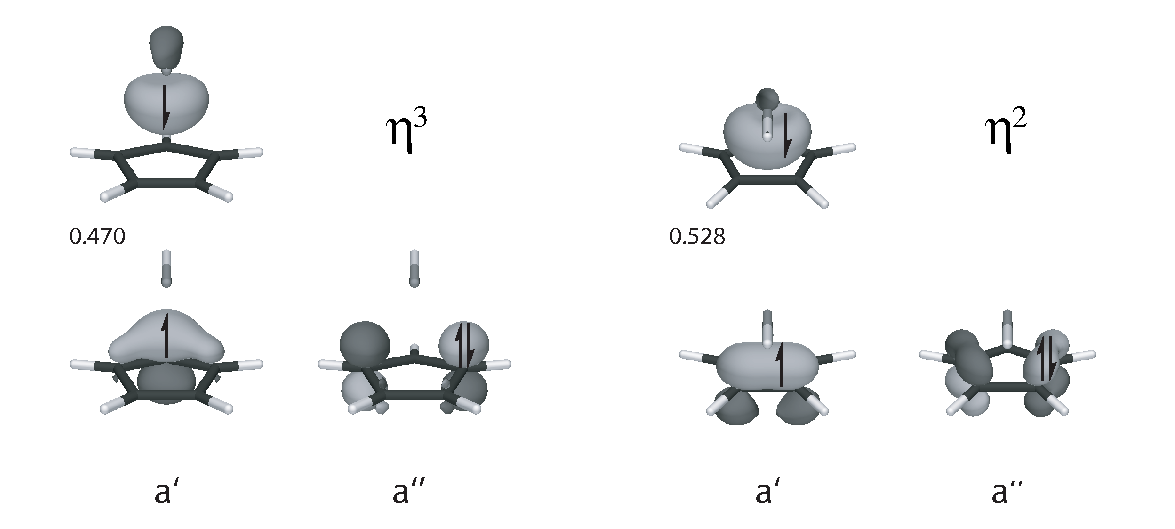
\includegraphics[scale=0.67]{cyclopentadienyl/figures/sih_sigma.eps}
\end{center}
\caption{Contour surfaces (amplitudes -0.1 (light) and 0.1 (dark)) of the two singly occupied spin-paired a\textquotesingle\ orbitals and the doubly occupied a\textquotesingle\textquotesingle\ orbitals for the $\eta^{3}$ (left) and $\eta^{2}$ (right) geometries of CpSiH. The numbers between the singly occupied orbitals are the orbital overlaps.}
\label{ch4.fig.sihs}
\end{figure}

\begin{figure} [htbp]
\begin{center}
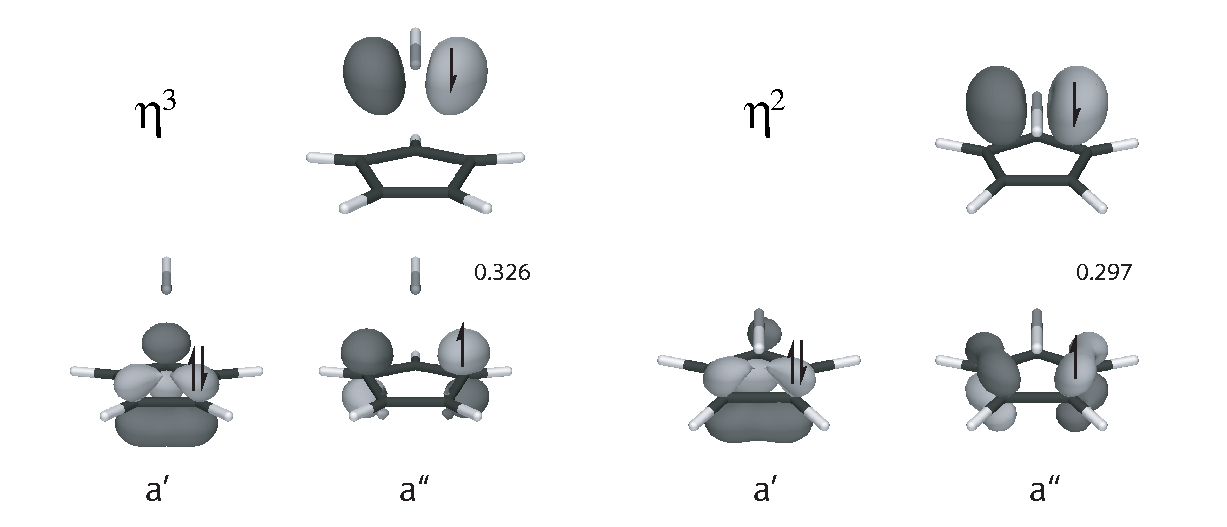
\includegraphics[scale=0.67]{cyclopentadienyl/figures/sih_pi.eps}
\end{center}
\caption{Contour surfaces (amplitudes -0.1 (light) and 0.1 (dark)) of the doubly occupied a\textquotesingle\ orbitals and the two singly occupied spin-paired a\textquotesingle\textquotesingle\ orbitals for the $\eta^{3}$ (left) and $\eta^{2}$ (right) geometries of CpSiH. The numbers between the singly occupied orbitals are the orbital overlaps.}
\label{ch4.fig.sihp}
\end{figure}

In Figure \ref{ch4.fig.sihs} the two singly occupied spin-paired a\textquotesingle\ orbitals on the left form the $\sigma$-like bond description for the $\eta^3$ geometry, the two singly occupied spin-paired a\textquotesingle\ orbitals on the right form the $\sigma$-like bond description for the $\eta^2$ geometry. The a\textquotesingle\textquotesingle\ orbitals are doubly occupied. In contrast, the a\textquotesingle\textquotesingle\ orbitals in Figure \ref{ch4.fig.sihp} are singly occupied and spin-coupled in a bond, while the a\textquotesingle\ orbitals on the Cp-ring are doubly occupied.

The shape of the a\textquotesingle\textquotesingle\ orbitals is independent of the occupation (compare the doubly occupied a\textquotesingle\textquotesingle\ orbitals in Figure \ref{ch4.fig.sihs} with their  singly occupied equivalents in Figure \ref{ch4.fig.sihp}). In contrast, the a\textquotesingle\ orbitals are different for both types of occupation, which is most clearly seen when the a\textquotesingle\ orbitals of the $\eta^3$ geometry are compared. The related a\textquotesingle\ orbital on the Cp-ring in the $\sigma$ geometry of CpSiH$_3$ (Figure \ref{ch4.fig.sih3}) is directed towards the silicon atom \textit{outside} the ring. This carbon atom in the Cp-ring of CpSiH$_3$ is rehybridized, because one hydrogen atom of the ring is lying out of the plane (the hydrogen at the back in Figures \ref{ch4.fig.slip_cpsih3} and \ref{ch4.fig.sih3}).

\begin{figure} [htbp]
\begin{center}
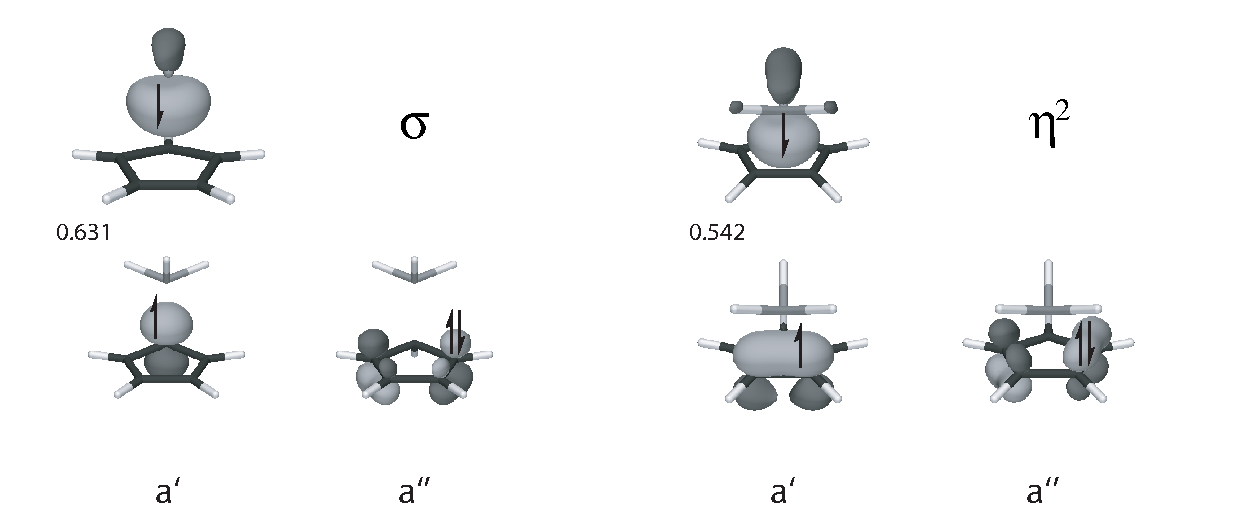
\includegraphics[scale=0.67]{cyclopentadienyl/figures/sih3_sigma.eps}
\end{center}
\caption{Contour surfaces (amplitudes -0.1 (light) and 0.1 (dark)) of the two singly occupied spin-paired a\textquotesingle\ orbitals and the doubly occupied a\textquotesingle\textquotesingle\ orbitals for the $\sigma$ (left) and $\eta^{2}$ (right) geometries of CpSiH$_3$. The numbers between the singly occupied orbitals are the orbital overlaps.}
\label{ch4.fig.sih3}
\end{figure}

The calculated orbital overlap values, presented in Table \ref{ch4.tab.overlaps}, together with the orbital pictures indicate that covalent bonding, both $\sigma$ and $\pi$-like between the Cp-ring and the metal, occurs in each contributing VB structure. In CpSiH the orbitals in the $\sigma$ structure overlap better in the $\eta^2$ geometry than in the $\eta^3$ geometry, 0.528 \textit{vs} 0.470 (see Figure \ref{ch4.fig.sihs}). On the other hand, in the $\pi$ structure the overlap in the $\eta^{3}$ geometry is higher than in the $\eta^{2}$ geometry, 0.326 \textit{vs} 0.297 (see Figure \ref{ch4.fig.sihp}).
\begin{table}[hbtp]
\caption{The orbital overlaps for the $\sigma$ and $\pi$ type of bonding of the MH$_x$ fragment to the ring. Overlaps are given for both geometries per molecule: $\eta^2$ for all three, $\eta^3$ for CpAlH$_2$ and CpSiH and $\sigma$ for CpSiH$_3$.}
\center
\begin{tabular}{|c|cc|cc|c|}
\hline
\textbf{Geometry}&
\multicolumn{2}{c|}{\textbf{CpAlH$_2$}}&
\multicolumn{2}{c|}{\textbf{CpSiH}}&
\textbf{CpSiH$_3$}\\
&
$\sigma$&
$\pi$&
$\sigma$&
$\pi$&
$\sigma$\\
\hline
$\eta^{2}$& 0.604 & 0.321 & 0.528 & 0.297 & 0.542 \\
$\eta^{3}$ / $\sigma$ & 0.578 & 0.382 & 0.470 & 0.326 & 0.631 \\
\hline
\end{tabular}
\label{ch4.tab.overlaps}
\end{table}

As shown in Table \ref{ch4.tab.weights}, the $\sigma$, $\pi$ and ionic structures of CpSiH and CpAlH$_2$ contribute significantly to the VB wave function. Obviously for CpSiH$_3$, only the $\sigma$ and ionic structures contribute. These weights suggest that the Cp-metal bond is a combination of \textit{covalent} and \textit{ionic} character and that the covalent character itself is partly $\sigma$ and partly $\pi$.
\begin{table}[htbp]
\caption{The weights \cite{coulson} of the structures ($\sigma$, $\pi$ and ionic as explained in Figures \ref{ch4.fig.sigma}-\ref{ch4.fig.ionic}) in the VB wave function.}
\center
\begin{tabular}{|c|ccc|}
\hline
\textbf{Molecule}&
\multicolumn{3}{c|}{\textbf{Weights}}\\
&$W_\mathrm{ion}$&
$W_\mathrm{\sigma}$&
$W_\mathrm{\pi}$\\
\hline
CpAlH$_2$ ($\eta^{2}$)&0.30&0.48&0.22\\
CpAlH$_2$ ($\eta^{3}$)&0.31&0.44&0.25\\
CpSiH ($\eta^{2}$)&0.29&0.41&0.30\\
CpSiH ($\eta^{3}$)&0.29&0.38&0.33\\
CpSiH$_3$ ($\sigma$)&0.26&0.74&-\\
CpSiH$_3$ ($\eta^{2}$)&0.34&0.66&-\\
\hline
\end{tabular}
\label{ch4.tab.weights}
\end{table}

Table \ref{ch4.tab.energies} contains the total energy ($E_\mathrm{tot}$), the energy for each separate structure ($E_\mathrm{ion}$, $E_\mathrm{\sigma}$ and $E_\mathrm{\pi}$) in the wave function and the Pauling resonance energy ($E_\mathrm{res}$) \cite{pauling}.
\begin{table}[hbtp]
\caption{The total energy ($E_\mathrm{tot}$) and the energy for each separate structure ($E_\mathrm{ion}$, $E_\mathrm{\sigma}$ and $E_\mathrm{\pi}$), and the resonance energy ($E_\mathrm{res}$), being the energy difference between the most stable single structure and the total energy \cite{pauling}. All energy values are in Hartrees, except the resonance energy, which is in kJ/mol. Values for the lowest single structure energy are printed in italics.}
\center
\begin{tabular}{|c|c|ccc|c|}
\hline
\textbf{Molecule}&
\textbf{Total}&
\multicolumn{3}{c|}{\textbf{Structure Energy}}&
\textbf{Resonance}\\
&
$E_\mathrm{tot}$&
$E_\mathrm{ion}$&
$E_\mathrm{\sigma}$&
$E_\mathrm{\pi}$&
$E_\mathrm{res}$ (kJ/mol)\\
\hline
CpAlH$_2$ ($\eta^{2}$)& -435.194422& -435.017811&\textit{-435.082625}&-434.996217&-293.5\\
CpAlH$_2$ ($\eta^{3}$)& -435.185474& -435.016456&\textit{-435.053468}&-434.992522&-346.6\\
CpSiH ($\eta^{2}$)&-481.590870&-481.403901&\textit{-481.451121}&-481.438667&-366.9\\
CpSiH ($\eta^{3}$)&-481.577254&-481.389228&-481.424327&\textit{-481.430267}&-385.9\\
CpSiH$_3$ ($\sigma$)&-482.783906&-482.534963&\textit{-482.740435}&-&-114.1\\
CpSiH$_3$ ($\eta^{2}$)&-482.726734&-482.545155&\textit{-482.661622}&-&-171.0\\ 
\hline
\end{tabular}
\label{ch4.tab.energies}
\end{table}
For both CpAlH$_2$ and CpSiH, the $\pi$-like valence bond structures have almost the same energy for the $\eta^{2}$ and $\eta^{3}$ arrangements. The $\sigma$-like valence bond structures are, however, significantly lower in energy in the $\eta^{2}$ arrangement, than in the $\eta^{3}$ arrangement. This suggests that $\sigma$ type bonding is most important in the $\eta^2$ arrangement and that it is the driving factor towards the $\eta^2$ geometry. This is also supported by the higher values of $W_\sigma$ for the $\eta^2$ than for the $\eta^3$ arrangement in Table \ref{ch4.tab.weights}. This is probably caused by the larger orbital overlap in the $\eta^2$ geometry: for CpSiH and CpAlH$_2$ it is 0.528 and 0.604 \textit{vs} 0.470 and 0.578 in the $\eta^3$ geometry, respectively (see Table \ref{ch4.tab.overlaps} for the overlaps). The better overlap is visible in the orbital plots for CpSiH in Figure \ref{ch4.fig.sihs}: since the orbital on the Cp ring in the $\eta^2$ geometry is more concentrated, \textit{i.e.} spread out over two instead of over three atoms in $\eta^3$, the overlap with the orbital on the metalhydride group is better. While for CpAlH$_2$ the ionic structures are intermediate in stability between the $\sigma$ and $\pi$ structures, for CpSiH the ionic structures are the least stable ones.

For CpSiH$_3$ the $\sigma$-like bond structure is \textit{much} more stable than the ionic structure. The $\sigma$-like bond structure is \textit{much} lower in energy for the $\sigma$ arrangement, due to the significantly larger orbital overlap ($\sigma$=0.631 $\eta^2$=0.542; Table \ref{ch4.tab.overlaps} and Figure \ref{ch4.fig.sih3}). In contrast to both CpAlH$_2$ and CpSiH, the SiH$_3$ fragment has a preference for the $\eta^3 / \sigma$ position above the Cp-ring. The reason for this could be the absence of the $\pi$-like structure (Figure \ref{ch4.fig.pi}) in CpSiH$_3$, despite its higher energy and lower weight for both CpAlH$_2$ and CpSiH. Despite the absence of the covalent $\pi$-like structure, the bond between the ring and the metal fragment in CpSiH$_3$ is more covalent in nature than the bond in CpAlH$_2$ and CpSiH. This is also corroborated by the higher ionization potential of the SiH$_3^{\bullet}$ fragment (0.361 Hartree) than of the AlH$_2^{\bullet}$ (0.274 Hartree) and the SiH$^{\bullet}$ (0.271 Hartree) fragments.

The resonance energies ($E_\mathrm{res}$) of CpAlH$_2$ and CpSiH range from \mbox{-293.5} kJ/mol for CpAlH$_2$ in the $\eta^2$ geometry to \mbox{-385.9} kJ/mol for CpSiH in the $\eta^3$ geometry. $E_\mathrm{res}$ values (Table \ref{ch4.tab.energies}) of CpSiH$_3$ are \mbox{-114.1} kJ/mol ($\sigma$ geometry) and \mbox{-171.0} kJ/mol ($\eta^2$ geometry). These values are roughly two to three times lower than the other resonance energies of the other geometries. This is in line with expectation: in CpSiH$_3$ there is only a single covalent structure, in the other two cases the covalent character is the combination of $\sigma$ and $\pi$ contributions. This means that neither the $\sigma$ contribution, nor the $\pi$ contribution on their own are representative for the covalent bonding, only the combination is. Therefore, the energy of the separate structures is relatively higher leading to a higher resonance energy. The resonance energy is the largest for the non-minimum geometries. In the traditional view of organic chemistry, a higher resonance energy indicates more thermodynamic stability. Here, however, the Lewis structures needed for the determination of resonance energy do not accurately describe the bonding situation for the transition state geometries.

The decomposition of the resonance energy in contributing resonances of the L\"{o}wdin orthogonalized structures \cite{havenith} is presented in Table \ref{ch4.tab.interactions}.
\begin{table}[htbp]
\caption{The decomposition of the resonance energy in orthogonalized structure contributions ($\epsilon_{ij}$), and the total resonance energy with respect to the weighted mean value of the energy of all structures ($E^m_\mathrm{res}$). All energy values are in kJ/mol.}
\center
\begin{tabular}{|c|ccc|c|}
\hline
\textbf{Molecule}&\multicolumn{3}{c|}{$\epsilon_{ij}$}&\textbf{Resonance}\\
&ionic-$\sigma$&ionic-$\pi$&$\sigma$-$\pi$&$E^m_\mathrm{res}$ (kJ/mol)\\
\hline
CpAlH$_2$ ($\eta^{2}$)& -560.14& -166.23& -174.30& -900.7\\
CpAlH$_2$ ($\eta^{3}$)& -531.33& -204.62& -212.94& -948.9\\
CpSiH ($\eta^{2}$)& -448.73& -171.12& -170.05& -789.9\\
CpSiH ($\eta^{3}$)& -413.44& -196.14& -182.37& -791.9\\

\hline
\end{tabular}
\label{ch4.tab.interactions}
\end{table}
For CpAlH$_2$ and CpSiH, the ionic-$\sigma$ interaction is two to three times higher than the ionic-$\pi$ and $\sigma$-$\pi$ interactions. This suggests that the ionic and the $\sigma$ structures separately are not representative for the bonding, but that the combination of these structures form the total bond picture. Thus, CpAlH$_2$ and CpSiH possess a polar $\sigma$ bond. Since in the case of CpSiH$_3$ only two structures contribute a decomposition is not necessary. Notwithstanding the large resonance energy in Table \ref{ch4.tab.energies} for CpSiH$_3$ is in line with the ionic-$\sigma$ resonance energy of CpAlH$_2$ and CpSiH. In all cases resonance between the $\pi$ structure with the other two structures is less important.

The difference in minimum geometry between CpSiH$_3$ ($\sigma$) and the other two molecules ($\eta^2$) is rationalized by the absence of a $\pi$-like bond structure in CpSiH$_3$. The extra possibility for CpAlH$_2$ and CpSiH to interact with the cyclopentadienyl moiety via the $\pi$-like bond structure, which has a significant weight (Table \ref{ch4.tab.weights}), structure energy (Table \ref{ch4.tab.energies}) and resonance with the other structures (Table \ref{ch4.tab.interactions}), leads to an enhanced stabilization. In the case that the AlH$_2$ or SiH fragment would occupy the $\sigma$ position, the overlap between the a\textquotesingle\textquotesingle\ orbitals would be negligible, and so would be the contribution of that structure.  

\section{Conclusions}

The present work shows that Valence Bond calculations based on three distinct VB structures (Figure \ref{ch4.fig.lewis}), being a superposition of a $\sigma$, a $\pi$ and an ionic structure result in distinguishable differences in the bond types, based on overlap, weight, structure, resonance and interaction energy.
\begin{figure}[htp]
\begin{center}
\includegraphics{cyclopentadienyl/figures/lewis.eps}
\end{center}
\caption{The three distinct Lewis structures, the ionic (\textbf{a}), the $\sigma$-like bond (\textbf{b}) and
the $\pi$-like bond (\textbf{c}).}
\label{ch4.fig.lewis}
\end{figure}
The $\sigma$-like bond structure is responsible for the general preference for $\eta^{2}$ geometry, since their energy in the $\eta^2$ geometry is significantly lower than in the $\eta^3$ geometry. Furthermore, the calculations indicate that for CpAlH$_2$ and CpSiH, although $\pi$ bonding is important (reflected in the weights for the $\pi$ structures ($W_\pi$)), it is not the main factor in causing the $\eta^{2}$ geometry, because the energy of the $\pi$ structures is almost equal for the $\eta^3$ and the $\eta^2$ geometry. 

The Hessian calculations for CpAlH$_2$, CpSiH and CpSiH$_3$ indicate that the $\eta^5$ geometry, in which the metal hydride moiety is placed above the middle of the ring, is a higher order saddle point and \textit{not} a transition state. For CpAlH$_2$ and CpSiH the $\eta^3$ geometry is the transition state between two $\eta^2$ minima and for CpSiH$_3$ the $\eta^2$ geometry is the transition state between two $\sigma$ minima.
%Alinea hieronder kwam uit de lucht vallen 6-1-2015.
%Our results, for example the shallow slippage curve for aluminum (Figure \ref{ch4.fig.slip_cpalh2}), have strengthened the believe that this type of molecule can be interesting for the storage of hydrogen for fuel cells \cite{himmel}. It corroborates with their finding of the Al-H bond longer than in typical Al$^{\textrm{III}}$ hydrides. Therefore, it is expected that it is relatively easy to release H$_2$ from this complex.

\section*{Acknowledgement}
We would like to thank Peter Budzelaar for his ideas and his work invested in the original review \cite{budzelaar} of which the valence bond section, rewritten in this chapter, was only a small part. We gratefully acknowledge partial financial support from NWO/NCF for use of supercomputer time on TERAS, SARA (The Netherlands, project number SG-032).  

\bibliography{cyclopentadienyl}
\bibliographystyle{../main/achemso}

\setcounter{chapter}{4}
\setcounter{NAT@ctr}{0}
\chapter{A Unified Orbital Model of Delocalized and Localized Currents in Monocycles, from Annulenes to Azabora-Heterocycles}
\label{chap_huckel}
\footnotetext{Reproduced with permission: ``A Unified Orbital Model of Delocalized and Localized Currents in Monocycles, from Annulenes to Azabora-Heterocycle'', \mbox{A. Soncini}, \mbox{C. Domene}, \mbox{J. J. Engelberts}, \mbox{P. W. Fowler}, \mbox{A. Rassat}, \mbox{J. H. van Lenthe}, \mbox{R. W. A. Havenith} and \mbox{L. W. Jenneskens}, \textit{Chem. Eur. J.} \textbf{2005}, \textit{11}, 1257-1266\ \ \ \textbf{www.chemeurj.org}\ \ \ \copyright 2005 Wiley-VCH Verlag GmbH \& Co. KGaA, Weinheim}

\ifthenelse{\boolean{wholethesis}}{\relax}{\begin{center}\textit{Generated on \today\ at \currenttime}\end{center}}

\noindent\textbf{Abstract:} Why are some $4n+2$ $\pi$ systems aromatic, and some not?  The ipsocentric approach to calculation of the current density induced in a molecule by an external magnetic field predicts a four-electron diatropic (aromatic) ring current for $4n+2$ $\pi$, and a two-electron paratropic (anti-aromatic) current for $4n$ $\pi$ carbocycles. With the inclusion of an electronegativity parameter, an ipsocentric frontier-orbital model also predicts the transition from delocalized currents in carbocycles to nitrogen-localized currents in alternating azabora-heterocycles, which rationalizes the differences in (magnetic) aromaticity between these iso-electronic $\pi$ conjugated systems.  \textit{Ab initio} Valence Bond calculations confirm the localization predicted by the na\"ive model, and coupled Hartree-Fock calculations give current-density maps that exhibit the predicted delocalized-to-localized/carbocycle-heterocycle transition.
\clearpage

\section{Introduction}
\lettrine{\initial{P}}{}lanar conjugated carbocyclic compounds show a strong link between $\pi$ electron count and molecular properties. H\"uckel's long-standing $4n+2$ rule distinguishes aromatic from anti-aromatic cycles, and correlates the energetics of these systems with their characteristic magnetic properties \cite{r01}. However, the periodic table offers wide possibilities for construction of iso-electronic heterocycles, and for many of them, direct transferability of the implied relationship between aromaticity and electron count is questionable or even counterfactual.  The replacement of CC by BN, for example, is known to lead to marked differences in magnetic properties \cite{r02}: the strong ring currents of the carbocycle vanish in the iso-electronic azabora-heterocycles, B$_{N/2}$N$_{N/2}$H$_N$ (\textbf{1}-\textbf{3}).  Herein we show that a simple frontier-orbital model of induced currents can in fact cope with both extremes, predicting the transition from delocalized to localized magnetic behavior that is found in full \textit{ab initio} current-density maps.
\begin{figure} [htp]
\begin{center}
\includegraphics[width=3.4in]{huckel/figures/scheme1.eps}
\end{center}
\end{figure}

The ipsocentric model \cite{r03,r04,r05} gives an accurate account of $\pi$ ring currents in planar carbocycles in terms of frontier-orbital contributions. The hallmarks of aromaticity and anti-aromaticity on the magnetic criterion \cite{r06,r07,r08,r09}, that is, the \textit{diatropic} currents of $4n+2$ systems and \textit{paratropic} currents \cite{r10} of planar $4n$ systems, are attributed in this model to four and two frontier electrons, respectively \cite{r04}. In both cases, the sense of the ring current follows directly from the symmetry properties of the HOMO--LUMO transition, and the predictions of a simple orbital theory are borne out in full \textit{ab initio} calculation of current-density maps \cite{r03,r04}. For the $4n+2$ heterocycles, borazine and boroxine, however, \textit{ab initio} maps show only \textit{localized} circulation of the $\pi$ electrons around the electronegative nuclei \cite{r02}.  How does the simple orbital model deal with this dichotomy?  In particular, why does it not predict ring currents for \textit{all} planar $4n$ and $4n+2$ $\pi$ systems? It is shown here that a generalization of the pictorial orbital model is able to account for both the presence of global currents in the carbocycles, and their absence in boron-nitrogen analogues such as borazine (\textbf{2}) and the eight-membered borazocine (\textbf{3}).

\section{Results and Discussion}

\subsection{The Aromaticity Analogy}

The considerations of magnetic aromaticity have their counterparts in the chemistry of these boron-nitrogen systems.  Although 6$\pi$ electron borazine (\textbf{2}) was originally called ``an inorganic benzene''\footnote{For recent summaries of the history of the discussion on the putative aromatic character of borazine, see, for example \cite{r11} and \cite{r11b}} and believed to have a resonance
energy similar to that of benzene, it was soon recognized that it had few reactions typical of aromatic systems.  For instance, borazine gives a tris-adduct with hydrogen chloride \cite{r12}. It is now generally agreed that borazine is not aromatic. In contrast to benzene, the $\pi$ electrons are localized on the more negative nitrogen atoms, even if some chemical behavior is reminiscent of that of benzene (e.g. formation of a weakly puckered hexaethylborazine tricarbonyl chromium complex) \cite{r13}.

The parent compounds B$_{N/2}$N$_{N/2}$H$_N$ with $N \ne 6$ have not been synthesized, although many derivatives of the homologues diazadiboretidine (also known as diazadiboretane, diazadiborete) (\textbf{1}) and borazocine (tetrazaborocine, tetrazaborocane) (\textbf{3}), have been prepared \cite{r14}. Interconversions between them (and with borazine) are possible, and their chemical properties differ strongly from those of the corresponding 4 $\pi$ and 8 $\pi$ carbocycles.  For instance, the four-membered ring survives thermal elimination of isobutene from a \textit{tert}-butyl derivative \cite{r14}.  Thus, in spite of their $4n$ $\pi$ electrons, these systems do not show the reactivity expected for an anti-aromatic molecule.  This again can be attributed to a localization of the $\pi$ electrons onto the more electronegative nitrogen atoms.  Similarly, energy calculations \cite{r11b,r15} suggest that \textbf{1} is less anti-aromatic than cyclobutadiene, in agreement with the H\"uckel prediction that
the anti-aromaticity in X$_2$Y$_2$H$_4$-type four-membered rings decreases with increasing electronegativity difference between X and Y \cite{r16}.  By using the ipsocentric model, we show here that diazadiboretidine (\textbf{1}), borazine (\textbf{2}) and borazocine (\textbf{3}) are in all fact \textit{non-aromatic}.

\subsection{Aromaticity, Ring Currents and Frontier Orbitals}

If aromaticity is to be defined by magnetic criteria \cite{r09}, then what is needed for its theoretical characterization is a reliable account of the currents induced by an external magnetic field, since susceptibility, nuclear shielding and other response properties are all integrals of this current density.  Realistic current-density maps can now be obtained by a computationally efficient procedure, the ipsocentric method, which avoids the gauge dependence problem by taking each point in space as an origin of the vector potential generating the magnetic field \cite{r17,r18}. This choice has the important conceptual advantage of yielding a unique decomposition into non-redundant orbital contributions \cite{r03}. The total current density is obtained as a sum over transitions from occupied to unoccupied orbitals, governed by symmetry rules, and modulated by energy denominators.

For a planar molecule in a perpendicular magnetic field, the symmetries determining the sense of circulation of the induced current about the molecular origin are those of in-plane translations ($T_x$, $T_y$) and the in-plane rotation, ($R_z$). A simple but powerful symmetry rule can be deduced. If the symmetry of a product of occupied and unoccupied orbitals contains that of $T_x$ or $T_y$, but not that of $R_z$, the contribution of the transition to the current has the \textit{diatropic} sense, and if it contains the symmetry of $R_z$, but not $T_x$ or $T_y$, the contribution has the reverse \textit{paratropic}, sense. If neither symmetry is present, the transition is inactive; if both, more detailed analysis is needed \cite{r03,r19}. On the magnetic criterion, the resultant of all such contributions determines aromaticity or anti-aromaticity (net diatropicity or paratropicity of ring current) of a monocycle. As the contributions are weighted by orbital energy \textit{differences}, frontier orbitals generally dominate.

\subsection{Currents in Carbocycles}

Current-density maps from \textit{ab initio} calculations \cite{r04} on the archetypal carbocycles, benzene and (planarized \cite{r20a,r20b}) cyclooctatetraene (COT) are shown in Figure \ref{ch5.fig.f01}. For each
molecule, the maps show total $\pi$ and $\sigma$ contributions to induced current density.  As expected, the currents arising from the $\pi$ electrons are respectively strongly diatropic in benzene and strongly paratropic in COT. Currents are dominated by HOMO contributions in both cases.
\begin{figure}
\begin{center}
\includegraphics[scale=1.3]{huckel/figures/fig1.eps}
\caption{Maps of the current density induced by a perpendicular external magnetic field in benzene (left) and
(planar) cyclooctatetraene (right).  Contributions of the $\pi$ (top) and $\sigma$ orbitals (bottom), calculated in the
RHF/6-31G$^{**}$ ipsocentric approach, plotted at one bohr above the molecular plane.  Anti-clockwise circulations
are diatropic, clockwise circulations paratropic. Carbon ($\bullet$) and hydrogen ($\odot$).}
\label{ch5.fig.f01}
\end{center}
\end{figure}

An angular momentum analysis shows how the symmetry rules account for these features. The H\"uckel $\pi$ molecular
orbitals of a cycle of $N$ identical atoms in full $D_{N\mathbf{h}}$ symmetry have well defined angular momentum properties
with respect to the principal axis. At each successive energy level, the quantum number, $\lambda (=0,1...,N/2)$,
increases by one. In a cycle with $N = 4n+2$ electrons, the HOMO and LUMO correspond to $\lambda = n$ and
$\lambda = n+1$, whereas for a cycle with $N = 4n$ electrons, in the closed-shell configuration obtained on
distortion to $D_{(N/2)\mathbf{h}}$ symmetry, the HOMO and LUMO derive from splitting of a pair of originally degenerate
orbitals with $\lambda = n$.

The canonical molecular orbitals are the \textit{delocalized} set ${\Psi_{\lambda,c/s}}$, producing uniform $\pi$ charge distribution on all C atoms. Functions {$\Psi_{\lambda,c}$} and {$\Psi_{\lambda,s}$} (degeneracy $d_\lambda$) have coefficients on center $r$ equal to $\sqrt{d_{\lambda/N}}\cos(2 \pi \lambda r/N)$ and $\sqrt{d_{\lambda/N}}\sin(2 \pi \lambda r/N)$, respectively \cite{r21}. Unless $\lambda = 0$ (or $N/2$, if allowed) the two functions share a single, well-defined angular momentum and are degenerate. For $\lambda = 0$ and $\lambda = N/2$, the sine partner vanishes identically. For other $\lambda$, the sine/cosine form is simply a choice that gives
convenient nodal properties.

When orbitals have well defined values of $\lambda$, the symmetry selection rules
for occupied-to-unoccupied transitions reduce to the following \cite{r04}: a diatropic contribution arises from a transition in which $\Delta\lambda = +1$, a paratropic contribution arises from a transition in which $\Delta\lambda = 0$. Thus, for a $4n+2$ cycle in maximum symmetry, only the HOMO--LUMO transition is active, and is responsible for the entire (4-electron) diatropic current. For a $4n$ cycle in the lower symmetry of the closed shell, two types of transition are active: the HOMO--LUMO transition leads to a 2-electron paratropic contribution, and HOMO-1--LUMO, HOMO--LUMO+1 to diatropic contributions.  Here, the smaller HOMO--LUMO splitting ensures dominance of the paratropic current. Decomposition of the carbocycle \textit{ab initio} $\pi$ maps into orbital contributions confirms the above analysis in detail \cite{r04}.

\subsection{A Model for Currents in Azabora-Heterocycles}

To adapt the pictorial molecular orbital analysis to the ipsocentric model for currents in the alternating heterocycles
such as borazine (\textbf{2}) and homologues \textbf{1} and \textbf{3}, it is sufficient to include one extra feature.
The method for dealing with heteroatoms in H\"uckel theory is to modify Coulomb and/or resonance integral parameters:
for B and N (as zero and two-electron donors), recommended parameters are $\alpha_B = \alpha -\beta$ and
$\alpha_N = \alpha + 1.5\beta$ \cite{r22a,r22b}. H\"uckel calculations using $\alpha_B = \alpha -1.1\beta$ and
$\alpha_N = \alpha + 1.5\beta$ have been reported for \textbf{1} to \textbf{3} \cite{r16}. The simplest model of an
equilateral B$_{N/2}$N$_{N/2}$H$_N$ cycle that allows for the differing electronegativities of B and N makes symmetrical
changes to the Coulomb parameters, that is, $\alpha_B = \alpha -\eta\beta$ and $\alpha_N = \alpha +\eta\beta$, where 
$\eta$ is positive.  Variation of the dimensionless quantity $\eta$ from $0$ to $\approx 1$ thus gives a one-parameter
model for correlating properties of annulenes and BN cycles.

The implications are now worked out in detail for six- and eight-cycles, as representatives of $4n+2$ and $4n$ $\pi$
systems, respectively.  Direct solution of the H\"uckel problem with modified $\alpha$ values gives energy levels {$\epsilon$}
and molecular orbitals {$\phi$}, from which consequences for ring currents can be deduced. In the limit $\eta = 0$,
the canonical molecular orbitals are {$\Psi_{\lambda,c/s}$}; when $\eta \ne 0$, they are linear combinations
of this starting set.

\subsubsection{Currents in the Six-Membered Cycle}

The secular equations for the alternating six-membered cycle
have maximal symmetry $D_{3\mathbf{h}}$ ($\eta \ne 0$) or $D_{6\mathbf{h}}$ ($\eta = 0$). The energies are ($D_{3\mathbf{h}}$ /$D_{6\mathbf{h}}$ labels,
$d_\lambda$ = degeneracy): 

\begin{math}
\\
\epsilon_0 = \alpha + \sqrt{4+\eta^2}\beta(\mathrm{A}_2''/\mathrm{A}_{2\mathrm{u}}), d_\lambda = 1;
\\
\\
\epsilon_1 = \alpha + \sqrt{1+\eta^2}\beta(\mathrm{E}''/\mathrm{E}_{1\mathrm{g}}), d_\lambda = 2;
\\
\\
\epsilon_2 = \alpha - \sqrt{1+\eta^2}\beta(\mathrm{E}''/\mathrm{E}_{2\mathrm{u}}), d_\lambda = 2;
\\
\\
\epsilon_3 = \alpha - \sqrt{4+\eta^2}\beta(\mathrm{A}_2''/\mathrm{B}_{2\mathrm{g}}), d_\lambda = 1.
\\
\\
\end{math}

When $\eta$ is non-zero, functions with different $\lambda$ are allowed to mix according to their symmetries in
the lower $D_{3\mathbf{h}}$ group, that is, in $\mathrm{A}_2''$, $\lambda = 0$ mixes with $\lambda = 3$, and in
$\mathrm{E}''$, $\lambda = 1$ mixes with $\lambda = 2$ (retaining the sine/cosine distinction).  As $\eta$
increases, the degree of mixing increases, and is described by angles $\mu$ and $\nu$, where
$\eta=2\tan2\mu=\tan2\nu$:

\begin{math}
\\
\phi_{0,c} = \cos \mu \psi_{0,c} - \sin \mu \psi_{3,c},
\\
\\
\phi_{1,c} = \cos \nu \psi_{1,c} - \sin \nu \psi_{2,c}, \phi_{1,s} = \cos \nu \psi_{1,s}+\sin \nu \psi_{2,s},
\\
\\
\phi_{2,c} = \sin \nu \psi_{1,c} + \cos \nu \psi_{2,c}, \phi_{2,s} = -\sin \nu \psi_{1,s}+\cos \nu \psi_{2,s},
\\
\\
\phi_{3,c} = \sin \mu \psi_{0,c} + \cos \mu \psi_{3,c}.
\\
\\
\end{math}

At $\eta= 0$, $\mu$ and $\nu$ are zero; in the limit of large $\eta$, the molecular orbitals of the alternating 6-cycle
become exact 50:50 mixtures, with $|\mu| = |\nu| = 45$\degrees. When $\eta=1$, $\phi_{1,c/s}$ still contains 95\% of the
benzene $\psi_{0,c}$  ($|\mu | = 13.3$\degrees), but the HOMO pair, $\phi_{1,c/s}$, contains a 15\% admixture of the
benzene LUMO,  $\psi_{2,c/s}$  ($|\nu| = 22.5$\degrees).  Figure \ref{ch5.fig.f02}(a) shows the correlation of orbitals and
energies with $\eta$ for the 6-cycle. H\"uckel $\pi$ charges reflect this shift with respect to the uniform charge distribution
of benzene, with \mbox{$1 \pm \frac{1}{2} (\frac{1}{\sqrt{5}} + \sqrt{2}) \approx 1.62$} and 0.38 $\pi$ electrons on the nitrogen and
boron atoms when $\eta=1$.  As $\eta$ increases, bonding orbitals concentrate onto electronegative nitrogen atoms, and
anti-bonding orbitals on the electropositive boron atoms, the functions becoming more ``localized''. 
\begin{figure}[htp]
\begin{center}
\includegraphics[scale=0.95]{huckel/figures/fig2.eps}
\end{center}
\caption{Correlation diagrams of energy and orbital composition in a H\"uckel model of \mbox{a) B$_3$N$_3$H$_6$,} 
\mbox{b) B$_4$N$_4$H$_8$} and \mbox{c) B$_2$N$_2$H$_4$,} as modeled by the single parameter $\eta$, where
$\alpha_\mathrm{B}=\alpha-\eta\beta$ and $\alpha_\mathrm{N}=\alpha+\eta\beta$. The graphs show the
variation of orbital energy, $x=(\epsilon-\alpha)/\beta$, with $\eta$.}
\label{ch5.fig.f02}
\end{figure}

The mixing has crucial consequences for predicted currents. At $\eta=0$, the dominant HOMO--LUMO transition responsible
for the ring current of the carbocycle is from {$\psi_{1,c},\psi_{1,s}$} to {$\psi_{2,c},\psi_{2,s}$}, for which $\Delta\lambda=1$; the
transition is therefore purely translational and contributes \textit{only} diatropic current.  For all $\eta>0$, as HOMO and LUMO
each contain $\lambda = 1$ and $2$ contributions, the transition includes $\Delta\lambda = 1$ and $0$ components, and the current
gains partial paratropic character.  The global diatropic current of benzene therefore weakens as $\eta$ increases.

A first interpretation of the effect of progressive orbital mixing on the ring current in a $4n+2$ cycle can be found by using
the simplest approach, the H\"uckel-London model \cite{r06}.  In this model, as formulated by McWeeny \cite{r23}, the ring current
per unit area of a cycle is proportional to the reduced bond current, $J_{rs}$, where $p_{rs}$ is the $\pi$ bond-order between
adjacent atoms $r$ and $s$ and $\overline{\pi}_{rs,rs}$ is the imaginary bond-bond polarizability \cite{r01}. 

\begin{math}
\\
J_{rs}=(p_{rs}+\beta\overline{\pi}_{rs,rs})\beta
\\
\end{math}

In a monocycle, $J$, $p$ and $\overline{\pi}$ are independent of the choice of adjacent pair. For benzene, $p=\frac{2}{3}$ and
$\overline{\pi}=-\frac{5}{9}\beta^{-1}$. For borazine with $\eta=1$, a straightforward calculation gives $p=\frac{1}{3}(\frac{2}{\sqrt{5}}+
\frac{1}{\sqrt{2}})$ and $\overline{\pi}=-\frac{1}{9}(\sqrt{5}+\frac{13}{4\sqrt{2}})\beta^{-1}$, from which the borazine:benzene
ratio of ring current intensity, assuming an equal ring area, is $(\frac{1}{\sqrt{5}}-\frac{1}{4\sqrt{2}})\approx 0.27$. This ratio
tends to zero as the electronegativity difference parameter $\eta$ tends to infinity. Thus, this crude model, in which current
is constrained to flow along the straight lines between adjacent atoms, predicts that an increase in $\eta$ leads to diminution
and eventual extinction of the global diatropic current. 

The picture can be refined by allowing for the spatial extent of the current outside the direct line of centers. The pseudo-$\pi$
model \cite{r24} includes explicit basis functions, and simulates $\pi$ ring currents by using a $\sigma$ model based on
the exact symmetry equivalence between the $\sigma$ orbitals of cyclic H$_N$ atoms and the $\pi$ orbitals of the
$N$-membered carbocycle. It turns out that ipsocentric \textit{in-plane} currents calculated for the H$_N$ system with
a minimal basis set give an excellent match to the \textit{out-of-plane} currents of the carbocycle calculated with a large
basis set. Figure \ref{ch5.fig.f03} presents a pseudo-$\pi$ simulation of the heterocyclic ring in which the boron and nitrogen
atoms are modeled by one-electron atoms with nuclear charges of $+0.7e$ and $+1.3e$, each carrying STO-3G $s$ and $p$
functions (exponent $1a_{0}^{2}$), the charge difference playing the role of the $\eta$ parameter in the H\"uckel analysis,
and the in-plane $p$ functions giving radial flexibility to charge and current densities. 
\begin{figure}[htp]
\begin{center}
\includegraphics{huckel/figures/fig3.eps}
\end{center}
\caption{\textit{Pseudo}-$\pi$ simulations of induced current density in B$_{N/2}$N$_{N/2}$H$_N$, with $N=6$ (left) and 
$N=8$ (right). In these molecules intense in-plane local circulations around the nitrogen centers in this pseudo-$\pi$ model
indicate out-of-plane $\pi$ circulations of similar strength. Here the symbol $\odot$ denotes the pseudo-hydrogen centers
representing the boron and nitrogen atoms in the model. Anti-clockwise circulations are diatropic, clockwise circulations
paratropic.}
\label{ch5.fig.f03}
\end{figure}
Pure symmetric arguments predicted
opposed paramagnetic and diamagnetic currents; the pseudo-$\pi$ map shows that they occupy different regions of space,
with diamagnetic circulation on the inside of the ring, the net effect being a set of circulations centered on electronegative atoms.
In the graph-theoretical H\"uckel-London model, this spatial pattern of opposed local currents was expressed as a reduction
of the sole available parameter, the bond current. Both models therefore essentially agree on the effect of the electronegativity
difference on the ring current.

\subsubsection{Currents in the Eight-Membered Cycle}

For the alternating eight-membered cycle, the maximal symmetry is $D_\mathrm{4h}$ ($\eta \ne 0$) or $D_\mathrm{8h}$
($\eta = 0$) and the energy levels $\varepsilon_{\lambda}$($D_\mathrm{4h}/D_\mathrm{8h}$ labels, $d_\lambda=$
degeneracy) are:

\begin{math}
\\
\varepsilon_0=\alpha+\sqrt{4+\eta^{2}}\beta \mathrm{(A_{2u}/A_{2u})}, d_\lambda=1;
\\
\\
\varepsilon_1=\alpha+\sqrt{2+\eta^{2}}\beta \mathrm{(E_{g}/E_{1g})}, d_\lambda=2;
\\
\\
\varepsilon_{2}^{\pm}=\alpha \pm \eta\beta \mathrm{(B_{1u}+B_{2u}/E_{2u})}, d_\lambda=2 \mathrm{\ at\ } \eta=0;
d_\lambda=1+1 \mathrm{\ at\ } \eta \ne 0;
\\
\\
\varepsilon_3=\alpha-\sqrt{2+\eta^{2}}\beta \mathrm{(E_{g}/E_{3g})}, d_\lambda=2;
\\
\\
\varepsilon_4=\alpha-\sqrt{4+\eta^{2}}\beta \mathrm{(A_{2u}/B_{2u})}, d_\lambda=1;
\\
\end{math}

In the carbocyclic system with full symmetry, the degeneracy of $\psi_{2,c}$ and $\psi_{2,s}$ leads to an open-shell configuration
which can be stabilized in various ways: distortion to $D_\mathrm{2d}$ leads to the tub-shaped equilibrium geometry of the free COT
molecule; in-plane relaxation to $D_\mathrm{4h}$ yields a geometry similar to those found in ``clamped''-substituted COT
systems \cite{r20a,r20b}. In spite of its bond alternation, planar $D_\mathrm{4h}$ COT retains fully delocalized orbitals and the ring
current of the equilateral carbocycle, as Figure \ref{ch5.fig.f01} shows \cite{r04,r20b}.

In the heterocyclic system, when $\eta \ne 0$, with the nitrogen atom as atom $0$, $\psi_{2,c}$ as the bonding and $\psi_{2,s}$
the anti-bonding partner, the assignment of labels B$_\mathrm{1u}$ and B$_\mathrm{2u}$ depends on the setting of $D_\mathrm{4h}$
within $D_\mathrm{8h}$. For a general value of $\eta$, the mixing of angular momentum components is again described by two
angles, $\mu$ and $\kappa$, with $\eta=2\tan 2 \mu = \sqrt{2} \tan 2 \kappa$.

\begin{math}
\\
\phi_{0,c} = \cos \mu \psi_{0,c} - \sin \mu \psi_{4,c},
\\
\\
\phi_{1,c} = \cos \kappa \psi_{1,c} - \sin \kappa \psi_{3,c}, \psi_{1,s} = \cos \kappa \psi_{1,s} + \sin \kappa \psi_{3,s},
\\
\\
\phi_{2,c} = \psi_{2,c}, \phi_{2,s} = \psi_{2,s},
\\
\\
\phi_{3,c} = \sin \kappa \psi_{1,c} + \cos \kappa \psi_{3,c}, \phi_{3,s} = - \sin \kappa \psi_{1,s} + \cos \kappa \psi_{3,s},
\\
\\
\phi_{4,c} = \sin \mu \psi_{0,c} + \cos \mu \psi_{4,c}.
\\
\end{math}

Note that functions $\psi_{2,c}$ and $\psi_{2,s}$, as the HOMO and LUMO, remain unmixed for all values of $\eta$, separated by a
gap that is linear in $\eta$, that is, $2\eta$. Each is perfectly localized, the HOMO on the nitrogen atom and the LUMO on the boron
atom. In contrast, with increasing values of $\eta$, the functions $\phi_{0,c}$, $\phi_{1,c}$, $\phi_{1,s}$, $\phi_{3,c}$, $\phi_{3,s}$ and
$\phi_{4,c}$ become increasingly localized on the electronegative atoms: when $\eta  = 1$, the nitrogen and boron atoms have
H\"uckel $\pi$ populations of \mbox{$1 \pm \frac{1}{2}(\frac{1}{2}+\frac{1}{\sqrt{3}}+\frac{1}{2\sqrt{5}}) \approx 1.65$} and $0.35$
electrons, respectively. When $\eta=1$, here representing planar B$_4$N$_4$H$_8$, $|\mu|=13.3$\degrees \ and
$|\kappa |=17.6$\degrees \ so that $\phi_{0,c}$ contains 5 \% of $\psi_{4,c/s}$ and HOMO--1 $\phi_{1,c/s}$ contains 10 \% of
$\psi_{3,c/s}$. Figure \ref{ch5.fig.f02}(b) shows the correlation of orbitals and energies with $\eta$ for the eight-membered cycle.
 
The symmetry argument for deducing the currents in $4n$ systems involves several steps. Initially ($\eta \approx 0$), the current is 
dominated by the HOMO--LUMO transition across a small energy gap. This $\Delta \lambda = 0$ transition generates an intense, purely
paratropic, ring current. As $\eta$ increases, the HOMO--LUMO gap opens, and the intensity of the current falls but remains paramagnetic.
Simultaneously, the separation of the \mbox{HOMO-1} and the LUMO and that of the HOMO and the LUMO+1, increase, but only slowly; both correspond
$\Delta \lambda = \pm 0$ diatropic contributions to current. Thus, as $\eta$ increases, the original global paratropic (anti-aromatic)
ring current is subject to intrinsic reduction and increasingly significant cancellation.

In the McWeeny form of the H\"uckel-London theory \cite{r23}, the ring current of the eight-membered cycle when $\eta$ is small is
dominated by the HOMO--LUMO contribution to the imaginary bond-bond polarizability, which is $-\frac{1}{16} \beta \eta$, and hence falls
sharply as $\eta$ increases from the planar-constrained form of COT (where $\eta=0$) to the heterocycle. When $\eta=1$, the
eight-membered cycle has $p=\frac{1}{2}(\frac{1}{\sqrt{3}}+\frac{1}{\sqrt{5}})$ and
$\overline{\pi}=-\frac{1}{8}(\frac{11}{3\sqrt{3}}+\frac{7}{2\sqrt{5}}+\frac{1}{2})\beta^{-1}$ to give bond currents
$J=\frac{\sqrt{3}}{72}+\frac{\sqrt{5}}{80}-\frac{1}{16}\approx -0.105$, which constitute a reduced but still net paratropic circulation.
If the ratio of the areas of the six- and eight-membered cycles is 9:16, a ring current of about a sixth of the strength of the
(diatropic) benzene current is implied. When, as for the six-membered cycles, the spatial extent of the current in the eight-membered
cycle is taken into account in a pseudo-$\pi$ calculation (Figure \ref{ch5.fig.f03}), the H\"uckel-London result is seen as a simplified
representation of the nitrogen-centered currents.

\subsubsection{Currents in the Four-Membered Cycle}

For the four-membered ring, B$_2$N$_2$H$_4$, the extinction of current with increasing $\eta$ follows the same pattern as that for the
eight-membered cycle. The four orbital energies are now $\epsilon_{0} = \alpha + \sqrt{4+\eta^{2}}\beta$,
$\epsilon_{1}^{\pm} = \alpha \pm \eta \beta$, again giving a linear HOMO--LUMO gap of $2\eta$ (see Figure \ref{ch5.fig.f02}c), and yielding
a paratropic current that weakens with $\eta$ and is increasingly cancelled by the diatropic current that arises from the transitions
across the HOMO--LUMO+1 and \mbox{HOMO-1}--LUMO gaps of $\eta+\sqrt{4+\eta^{2}}\beta$. In the H\"uckel-London theory, when $\eta=1$ the reduced
bond current for the four-membered ring remains net paratropic ($J=\frac{1}{4\sqrt{5}}; -0.138$) and corresponds to half the current
of a benzene ring which has $\frac{9}{4}$ times the area, and again represents the pattern of nitrogen-centered circulations in a more
detailed description.

\subsubsection{Generalization for $4n$ and $4n+2$ $\pi$ BN Heterocycles}

The results for the four-, six- and eight-membered cycles are generalizations for the $4n$ and $4n+2$ $\pi$ BN heterocycles, with
separate mechanisms, but equivalent results for the ring current in both cases. Consider an $[N]$-carbocycle, where $N$ is even.
As $\eta$ increases from 0, each bonding ($b$)/anti-bonding($a$) molecular orbital pair of the parent bipartite carbocycle, with angular
momenta $\Lambda_{b}$ and $\Lambda_{a}=N/2 - \Lambda_{b}$, which correspond to equal but opposite eigenvalues, mix to form a 
bonding/anti-bonding pair in the $[N]$-center BN heterocycle with energies $x_b = \sqrt{4\cos^{2}\tau_{\Lambda_b}+\eta^2}$ and
$x_a = -\sqrt{4\cos^2 \tau_{\Lambda_{a}}+\eta^2}$, where $\tau_\Lambda=2\pi\Lambda/N$, so that $x_b=-x_a$. The rotation describing the
mixing is parametrized by the angle $\omega_\Lambda=\frac{1}{2}\tan^{-1}(\eta/2\cos\tau_\Lambda)$, where $0 \le \omega_\Lambda \le \pi/4$.

When $N=4n+2$, $\Lambda_\mathrm{HOMO}=n$ and $\Lambda_\mathrm{LUMO}=n+1$, and the mixing angle $\omega_\Lambda$ is maximal for a given
value of $\eta$. As we have seen, this leads to a sufficiently large value of $\eta$ to disrupt the global ring current and eventual
localization. When $N=4n$, $\Lambda_\mathrm{HOMO}=\Lambda_\mathrm{LUMO}=n$, the original HOMO and LUMO carbocycle eigenfunctions remain
unmixed. Disruption of the global paratropic ring current is caused by the widening of the HOMO--LUMO gap, triggering cancellation of
the rotational HOMO--LUMO and translational \mbox{HOMO-1}--LUMO contributions.

\subsection{\textit{Ab Initio} Current-Density Maps in Azabora-Heterocycles}

To obtain \textit{ab initio} data on the currents in BN analogues of the $4n$ and $4n+2$ carbocycles, calculations were performed on B$_2$N$_2$H$_4$,
B$_3$N$_3$H$_6$ and B$_4$N$_4$H$_8$. The geometry of each molecule was optimized at the restricted Hartree-Fock (RHF) level with the 
6-31G** basis set and currents were calculated by using the ipsocentric approach at the coupled Hartree-Fock (CHF) level with the same
basis set. At this level of theory, B$_3$N$_3$H$_6$ and B$_4$N$_4$H$_8$ have planar structures with $D_\mathrm{3h}$ and $D_\mathrm{4h}$ symmetries,
respectively, whereas the planar structure of B$_2$N$_2$H$_4$ with $D_\mathrm{2h}$ symmetry is a transition state (imaginary frequency 116$i$
cm$^{-1}$) that leads to a shallow $C_\mathbf{2v}$ butterfly optimum, hinged at the BB diagonal, with a dihedral angle of 167\degrees.
Current-density maps were computed for both the constrained planar and the fully optimized structures of B$_2$N$_2$H$_4$. An alternative
geometry for B$_4$N$_4$H$_8$ is based on the occupation of the corners of a cube \cite{r25a}; this compact structure is slightly preferred
to the planar form, as determined with small basis sets \cite{r25b}, but lies 302 \mbox{kJ mol$^{-1}$} above it when calculated at the 6-31G**
level. All three planar molecules have uniform BN distances ($R$=1.4432, 1.4258, 1.4254 \AA, respectively).

These geometries are in general agreement with available experimental and theoretical data. The non-planarity of B$_2$N$_2$H$_4$ has been
noted in previous \textit{ab initio} calculations \cite{r26}, which gave a BN distance of 1.457 \AA, and although the parent molecule itself has not
been synthesized, X-ray structures of five substituted molecules \cite{r14} are known with mean BN distances varying between 1.430 and
1.486 \AA, and all are planar apart from the severely hindered tetra-\textit{tert}-butyl derivative. Borazine has been the subject of many
\textit{ab initio} calculations \cite{r27a,r27b,r27c,r27d,r27e,r27f}. The RHF/6-31G**-calculated BN distance of 1.4258 \AA\ in borazine compares with
1.4355$\pm$0.0021 \AA\ (gas electron diffraction \cite{r28a,r28b} and 1.429 \AA\ (X-ray \cite{r28c}). No experimental data are available for
parent B$_4$N$_4$H$_8$, but experimental and theoretical structural data on its derivatives have been reviewed by Gilbert and Gailbreath \cite{r26}.
Calculations at different levels give a planar (B3LYP/6-31$^{+}$G*) or near-planar (MP2/6-31$^{+}$G*) structure for B$_4$N$_4$H$_8$ with a BN length of
1.436 \AA, intermediate between single and double bonds. Equivalent calculations on the permethylated monocycle show it to adopt a tub
structure \cite{r26}. X-ray structures for derivatives with bulky substituents are tub-like with alternating bonds as in, for example,
(\textit{t}BuN)$_4$(MeB)$_4$ \cite{r29}. Solution ${}^1$H NMR spectra of B$_4$N$_4$(CH$_2$R)$_4$(Me)$_4$ show a non-planar eight-membered
ring \cite{r30}.

The current densities induced in (planar) B$_2$N$_2$H$_4$, B$_3$N$_3$H$_6$ and B$_4$N$_4$H$_8$ by a perpendicular magnetic field are plotted in Figure \ref{ch5.fig.f04}.
\begin{figure}[htp]
\begin{center}
\includegraphics{huckel/figures/fig4.eps}
\end{center}
\caption{Current density induced by a perpendicular external magnetic field in the molecules B$_2$N$_2$H$_4$ (\textbf{1}, planar), B$_3$N$_3$H$_6$ (\textbf{2}), B$_4$N$_4$H$_8$ (\textbf{3}) (left to
right), partitioned as contributions from (top to bottom) the \mbox{HOMO-1}, HOMO, $\pi$ and $\sigma$ orbitals, calculated by the RHF/6-31G** ipsocentric approach. Where the \mbox{HOMO-1} and HOMO are degenerate, the map shows the summed contribution of the pair. Contributions are plotted at one bohr above the molecular plane. Anti-clockwise circulations are
diatropic, clockwise circulations paratropic. Nitrogen, boron and hydrogen centers are denoted by circles containing a bar, cross or dot, respectively.}
\label{ch5.fig.f04}
\end{figure}
For each molecule, the maps show HOMO, \mbox{HOMO-1} and the total $\pi$ and $\sigma$ contributions to the induced current density plotted in a plane one bohr above
that of the nuclei. As Figure \ref{ch5.fig.f04} shows, all three systems, in contrast to the carbocycles, have multi-center patterns of local diatropic $\pi$ circulations centered on the
nitrogen atoms. In B$_3$N$_3$H$_6$, the nitrogen-centered $\pi$ circulations arise entirely from the four electrons of the doubly degenerate HOMO:
the total $\pi$ and HOMO maps are visually indistinguishable, and the contribution of the \mbox{HOMO-1} is negligible. In B$_2$N$_2$H$_4$ and B$_4$N$_4$H$_8$, the
nitrogen-centered $\pi$ circulations arise from a combination of the inner paratropic HOMO and the outer diatropic \mbox{HOMO-1} currents. As the localized
$\sigma$ and $\pi$ currents rotate in the same sense, they are reinforced in all three molecules. Maps of total current density (not shown) plotted for the puckered optimum
geometry of B$_2$N$_2$H$_4$ at a height of 1 $a_0$ above the nitrogen atoms and parallel to the median nuclear plane show the same general features:
the localized nature of the current density is not critically dependent on planarity.

\subsection{Localized Orbital Analysis}
Further analysis using Pipek-Mezey localization of the canonical molecular orbitals \cite{r31} demonstrates the strong generic similarity of all three systems.
The localized orbitals of B$_{N/2}$N$_{N/2}$H$_N$ are $N$ core $1s$ orbitals on the heavy atoms, $N/2$ BN localized $\sigma$ bonding orbitals,
$N/2$ NH and $N/2$ BH localized $\sigma$ bonding orbitals and $N/2$ $\pi$ orbitals that are essentially nitrogen-localized $\pi$ lone
pairs. In this analysis nitrogen-centered $\pi$ currents arise naturally as circulations in the lone pairs. The $\sigma$ currents shown
in Figure \ref{ch5.fig.f04} for B$_2$N$_2$H$_4$, B$_3$N$_3$H$_6$ and B$_4$N$_4$H$_8$ have nodes at the boron sites. In the localized-orbital picture, the prominent
``triangular'' diatropic circulations around the nitrogen atoms arise from the three bonds meeting at nitrogen, each
deltoid constituting a six-electron diatropic circulation. In the carbocycles, the $\sigma$ currents are more uniformly distributed
over all the heavy atoms, but are still spatially localized \cite{r32}. The main difference in the magnetic response between
carbocycles and azabora-heterocycles is that the $\pi$ ring currents of one class are absent in the other. This distinction
is clear from the computed current-density maps, which are fully compatible with the qualitative analysis based
on symmetry and electronegativity. One and the same ipsocentric molecular orbital picture explains both the current in
the carbocycle and the lack of current in the heterocycle.

\subsection{Valence Bond Calculations on Azabora-Heterocycles}
As the localization of density on electronegative nitrogen centers is a key factor in the simple H\"uckel model of ring current
quenching, it is important to verify this qualitative difference between carbocyclic and azabora-heterocyclic systems
by using more sophisticated theoretical methods. Accordingly, \textit{ab initio} Valence Bond Configuration Interaction (VBCI)
calculations, in which many structures are used, and Valence Bond Self Consistent Field (VBSCF) \cite{r33} calculations, in
which both orbitals and structure coefficients are optimized, were performed on planar B$_2$N$_2$H$_4$ (\textbf{1}), B$_3$N$_3$H$_6$ (\textbf{2}) and
B$_4$N$_4$H$_8$ (\textbf{3}) with the 6-31G** basis set. All were carried out by using TURTLE \cite{r34}, as implemented in the GAMESS-UK
package \cite{r35}.

The wave function in the Valence Bond calculations consists of a Hartree-Fock $\sigma$ core in structures with singly occupied
$\pi$ orbitals. From a chemical point of view, these different structures can be seen as different bonding arrangements.
All possible structures that can be generated by using the occupied atomic orbitals were used in the VBCI
wave function, including chemically irrelevant ones. For B$_2$N$_2$H$_4$ there are 20 possible structures which arise from the
20 ways of distributing four electrons over four $p$ orbitals to give a singlet. For B$_3$N$_3$H$_6$ 175 structures are possible, and
for B$_4$N$_4$H$_8$ there are 1764. A VBCI calculation will show which bonding arrangements are preferred.
However, the VBCI wave function, owing to its fixed atomic orbital basis set, does not present a compact description
of the wave function as orbital optimization and correlation effects are intermixed. Therefore the most important
structures in the VBCI calculations were used to construct a VBSCF wave function without imposing restrictions on the
orbitals. From the coefficients in the VBCI wave functions the weights \cite{r36}, and thus the importance of each structure,
may be derived. For \textbf{1}-\textbf{3}, the most important structure types are shown in Figure \ref{ch5.fig.f05} with their respective weights.
\begin{figure}
\begin{center}
\includegraphics[scale=0.98]{huckel/figures/fig5.eps}
\end{center}
\caption{The most significant symmetry-distinct VBCI structures of
B$_2$N$_2$H$_4$ (\textbf{1}), B$_3$N$_3$H$_6$ (\textbf{2}) and B$_4$N$_4$H$_8$ (\textbf{3}) with the total weight of the combined
set in parentheses.}
\label{ch5.fig.f05}
\end{figure}
From these weights it appears that several structures contribute to the total wave function.

Subsequently, for B$_2$N$_2$H$_4$, the sets of structures of each kind were separately optimized in VBSCF calculations without imposing any
restrictions on the orbitals. The resulting energies of the first (\textbf{1a}:  160.722209 $E_\mathrm{h}$) and the second
(\textbf{1b}:  160.721245 $E_\mathrm{h}$) were very similar, with the first structure, having two different orbitals on each nitrogen atom
(see Figure \ref{ch5.fig.f06}), slightly more favorable.

\begin{figure}
\begin{center}
\includegraphics{huckel/figures/fig6.eps}
\end{center}
\caption{The singly occupied $p$ orbitals of B$_2$N$_2$H$_4$ (\textbf{1}), B$_3$N$_3$H$_6$ (\textbf{2}) and B$_4$N$_4$H$_8$ (\textbf{3}), respectively,
which correspond to the structures \textbf{1a}, \textbf{2a} and \textbf{3a} (see Figure \ref{ch5.fig.f05}). Orbitals from the left and right of the picture together
form the correlated lone pair on the nitrogen atom.}
\label{ch5.fig.f06}
\end{figure}

A VBCI calculation was then performed on the first two sets of structures (\textbf{1a}+\textbf{1b}), each with their own optimized
orbitals. This calculation gave the same energy as the single structure VBSCF calculation (\textbf{1a}), whereas the overlap between
set one (\textbf{1a}) and set two (\textbf{1b}) was over 99.9\%. This means that the VBSCF calculations converge to the same
wave function, which is most aptly described as nitrogen atoms, each with a correlated pair of $\pi$ electrons. The conclusion
is that there is no resonance energy and thus no resonance \cite{r37}. Similar results were obtained for B$_3$N$_3$H$_6$ (\textbf{2}) \cite{r37}
and B$_4$N$_4$H$_8$ (\textbf{3}).

These calculations show the same tendency as both the H\"uckel and the ring current calculations, that is, localization
of electrons on the nitrogen atoms. In fact, the Valence Bond results show that the ground states of B$_2$N$_2$H$_4$ (\textbf{1}), B$_3$N$_3$H$_6$
(\textbf{2}) and B$_4$N$_4$H$_8$ (\textbf{3}) correspond to the structures \textbf{1a}, \textbf{2a} \cite{r37} and \textbf{3a}, respectively.

\section{Conclusions}

Given the success of the simple one-parameter model in pointing out qualitative differences in current patterns between
carbo- and azabora-cycles, it is natural to ask about its predictions for other systems, for example, X$_{N/2}$Y$_{N/2}$H$_N$-
where does the borderline between ``aromatic'' and ``non-aromatic'' occur in this picture? The crudest form of the
model shows a change from global circulation to localized currents by a strong reduction in the magnitude of ring current
from $\eta$=0 to $\eta$=1; this variation is sigmoidal (Figure \ref{ch5.fig.f07})
\begin{figure}
\begin{center}
\includegraphics{huckel/figures/fig7.eps}
\end{center}
\caption{
Variation of ring current, $j$, with electronegativity parameter, $\eta$,
in the H\"uckel-London treatment of the X$_3$Y$_3$ cycle. $j(\eta)$ is the ring current
for a regular hexagonal cycle with alternating coulomb parameters
$\alpha \pm \eta \beta$ as a percentage of the current for the same cycle with $\eta$=0. The
inset curve (not to scale) shows the variation of the first derivative d$j(\eta)$/d$\eta$ near $\eta$=0.5.
}
\label{ch5.fig.f07}
\end{figure}
with a point of inflection, where current will be most sensitive to variation in $\eta$, at $\eta \approx$ 0.5, where $\eta$ represents the deviation
from the average electronegativity, that is, $| \alpha_\mathrm{X}- \alpha_\mathrm{Y} | 2\beta$. A rule of thumb is that $\alpha_\mathrm{X}$
varies with the difference in electronegativity between X and C: $(\alpha_\mathrm{X} - \alpha_\mathrm{C})/\beta \approx \chi_\mathrm{X}-\chi_\mathrm{C}$
for X as a one-electron donor and  $(\alpha_\mathrm{X} - \alpha_\mathrm{C})/\beta \approx 1 + \chi_\mathrm{X}-\chi_\mathrm{C}$ as a two-electron
donor \cite{r22a}. Inflection at $\eta\approx$ 0.5 is consistent with indications for X$_3$Y$_3$ 6$\pi$ systems from ring current maps \cite{r02} and
NICS calculations \cite{r27c}: systems in which the electronegativity/coulomb-parameter difference between X and Y is 1 or
more on the Pauling scale lack ring currents (B$_3$O$_3$H$_3$ \cite{r02,r27c}, B$_3$N$_3$H$_6$ \cite{r02,r27c}, Al$_3$N$_3$H$_6$ \cite{r27c} and
Al$_3$P$_3$H$_6$ \cite{r27c}), whereas those with differences of half a unit or less may (C$_3$N$_3$H$_3$ \cite{r02,r27c} and B$_3$P$_3$H$_6$ \cite{r27c})
or may not (B$_3$S$_3$H$_3$ \cite{r27c}) show global currents. This uniform trend lends support to the expectation that orbital-based models should be able to
account for the subtleties of ring current in the range of aromatic, non-aromatic and anti-aromatic heterocycles, and is a strong argument for
using methods in which the orbital contributions themselves have a clear physical basis.

\section*{Addendum}
It has been a decade ago that this chapter was published as article in Chemistry -- A European Journal. It is, therefore, timely to have a look at the literature regarding azabora-hetrocycles and the methods used to investigate (their) aromaticity.



\section*{Acknowledgements}
L.W.J. acknowledges financial support from the Royal Society of Chemistry's Journals Grants for International Authors Programme (0301433).
R.W.A.H. acknowledges financial support from the Netherlands Organization for Scientific Research (NWO), grant 700.53.401. P.W.F, A.R. and
A.S. thank the EU for financial support from the Framework V programme (RTN Contract HPRN-CT-2002-00136 ``WONDERFULL'').
C.D. thanks the Royal Society for a University Research Fellowship and P.W.F. for a Royal Society/Wolfson Research Merit Award.

\bibliography{huckel}
\bibliographystyle{../main/achemso}

\setcounter{chapter}{5}
\setcounter{NAT@ctr}{0}
\chapter{The Electronic Structure of Inorganic Benzenes: Valence Bond and Ring Current Descriptions}
\footnotetext{Reproduced with permission from ``The Electronic Structure of Inorganic Benzenes: Valence Bond and Ring Current Descriptions'', \mbox{J. J. Engelberts}, \mbox{R. W. A. Havenith}, \mbox{J. H. van Lenthe}, \mbox{L. W. Jenneskens} and \mbox{P. W. Fowler}, \textit{Inorg. Chem.} \textbf{2005}, \textit{44}, 5266-5272. \  \ \ \copyright\ 2005 American Chemical Society.}
\label{chap_inorganic}

\ifthenelse{\boolean{wholethesis}}{\relax}{\begin{center}\textit{Generated on \today\ at \currenttime}\end{center}}

\noindent\textbf{Abstract:}  Valence Bond (VB) theory and ring current maps have been used to study the electronic structure of inorganic benzene analogues X$_6$H$_6$ (X=C(\textbf{1}), Si (\textbf{2})),
X$_6$ (X=N(\textbf{3}), P(\textbf{4})), X$_3$Y$_3$H$_6$ (X,Y = B,N
(\textbf{5}), B,P (\textbf{6}), Al,N (\textbf{7}), Al,P (\textbf{8})) and
B$_3$Y$_3$H$_3$ (Y=O(\textbf{9}), S(\textbf{10})).
It is shown that the homonuclear compounds possess benzene-like character, with
resonance between two Kekul\'e-like structures, and induced diatropic
ring currents. Heteronuclear compounds typically show localization of the
lone-pairs on the electronegative atoms; Kekul\'e-like structures do not
contribute. Of the heteronuclear compounds, only B$_3$P$_3$H$_6$ (\textbf{6})
has some benzene-like features with a
significant contribution of two Kekul\'e-like structures to its VB wave
function, an appreciable resonance energy, and a discernible diatropic
ring current in planar geometry. However, relaxation of \textbf{6} to the optimal non-planar
chair conformation is accompanied by onset of localization of ring current.

\newpage

\section{Introduction}

\lettrine{\initial{B}}{}enzene is the archetypal example of a molecule that possesses remarkable
physical properties arising from its delocalized $\pi$ electrons.
Historically, chemists have searched for other molecules that resemble
benzene. Borazine (B$_3$N$_3$H$_6$ (\textbf{5})) and boroxine (B$_3$O$_3$H$_3$ (\textbf{9}))
are examples that have been proposed: in geometry and formal topology of the
$\pi$ molecular orbitals both are similar to benzene. However, the question of
whether their $\pi$ electrons are delocalized in the same sense as they are in
benzene (resonance between two Kekul\'e structures), is less clear. 

Aromaticity has many definitions.
Bond length equalization \cite{arom1}, extra energetic
stabilization \cite{arom2} with respect to an often hypothetical reference
system, and the ability to sustain an induced diatropic ring current \cite{ring4,ring1,ring2,ring3,nics}
have all been proposed as
descriptors for aromaticity. Many studies have been devoted to the aromaticity
of benzene analogues using concepts of aromatic stabilization energy (ASE),
exaltation of diamagnetizability $\Lambda$, and Nucleus Independent Chemical
Shift (NICS \cite{nics}) \cite{fink,jemmis,cooper,fowler1,schleyer1,soncini1}. On
these criteria, ``inorganic benzenes'' such as borazine (B$_3$N$_3$H$_6$ (\textbf{5})),
boroxine (B$_3$O$_3$H$_3$ (\textbf{9})) and borthiin (B$_3$S$_3$H$_3$ (\textbf{10})) are non-aromatic,
whereas $s$-triphosphatriborin (B$_3$P$_3$H$_6$ (\textbf{6})), hexaazabenzene (N$_6$ (\textbf{3})),
hexaphosphabenzene (P$_6$ (\textbf{4})), and hexasilabenzene (Si$_6$H$_6$ (\textbf{2})) are of modest
aromatic character \cite{schleyer1}.

An important question is whether the electronic structure of an inorganic
benzene expressed in terms of Lewis structures resembles that of benzene
itself. Valence Bond (VB) theory \cite{heitler}, where a molecular wave
function is constructed from atomic states, offers an interpretation precisely
in terms of resonating Lewis structures \cite{lewis}. Weights can be attributed
to these structures, using a formula proposed by Chirgwin and Coulson to assess
their importance in the total wave function \cite{chirgwin}. Furthermore, VB
provides a resonance energy ($E_{\mathrm{res}}$) of a molecule, as
defined by Pauling \cite{pauling}; this is the difference between the
total energy ($E_{\mathrm{tot}}$) and that of the most stable
structure. For benzene itself, a large value of 
$E_{\mathrm{res}}$=85--190 kJ/mol with respect to one
structure is found \cite{benzbovb,nature,fokke}. The structure with the lowest energy is
of the Kekul\'e type and has the largest weight in the wave function. Thus,
for benzene (\textbf{1}), aromaticity is characterized not only by a high
resonance energy, but also by large weights of the Kekul\'e
structures in the wave function.

In contrast, for the heteronuclear analogues borazine (\textbf{5}) and boroxine (\textbf{9}),
spin-coupled Valence Bond calculations indicate that only one Lewis structure,
corresponding to a description of three lone-pairs localized on the
electronegative centers, is important in the wave function, and
$E_{\mathrm{res}}$ is negligible \cite{cooper}. Significantly, the negligible
resonance energy coincides with the absence of a diatropic $\pi$ ring current, and so
energetic and magnetic criteria of aromaticity are in agreement here \cite{fowler1}.

The aim of the present chapter is to explore the parallels between the
energetic and magnetic criteria of aromaticity for a series of inorganic
benzenes, using VB methods for evaluation of resonance energy ($E_\mathrm{res}$), and
distributed origin computation of induced current density to establish
presence or absence of ring currents. VB calculations are performed using both
the strictly atomic model and the spin-coupled method. The magnetic response treatment is
carried out at the coupled Hartree-Fock
level \cite{ctocd-dz2,ctocd-dz3} using the ``ipsocentric''
 \cite{big,small} CTOCD-\textit{DZ} \cite{ctocd-dz4} approach, which is derived from the CSGT
method of Keith and Bader \cite{ctocd-dz1}, and which provides maps of induced
current density that give detailed information about the nature and
distribution of currents, and rationalize other magnetic indices of
aromaticity.

A set of candidate inorganic benzenes was defined (with benzene itself
included for comparison) as: X$_6$H$_6$ (X=C(\textbf{1}), Si (\textbf{2})),
X$_6$ (X=N(\textbf{3}), P(\textbf{4})), X$_3$Y$_3$H$_6$ (X,Y = B,N
(\textbf{5}), B,P (\textbf{6}), Al,N (\textbf{7}), Al,P (\textbf{8})) and
B$_3$Y$_3$H$_3$ (Y=O(\textbf{9}), S(\textbf{10})). Computed data on electric \cite{lazzeretti}
and magnetic \cite{schleyer1} properties of some of the molecules in the set are available
in the literature, including a
full set of NICS(0) \cite{nics} values for all molecules studied here.    

\section{Computational Details}

\subsection{Geometry Optimization}

Geometries of the molecules were optimized with GAMESS-UK  \cite{gamess} at the
DFT level, using the B3LYP functional (Table \ref{ch6.table1}) \cite{b3lyp1,b3lyp2,b3lyp3}.
\begin{table}[htp]
\caption{Energetic and structural data for the set of candidate inorganic benzenes.}
\begin{center}
\begin{tabular}{c r r r c c}
\hline
\textbf{Compound}&
\textit{R}(\AA)${}^{a}$& 
$E_{\mathrm{tot,B3LYP}}$ ($E_{\mathrm{h}}$)${ }^{b}$&
$E_{\mathrm{tot,RHF}}$ ($E_{\mathrm{h}}$)${ }^{c}$ &
\mbox{n$_{\mathrm{imag}}$}${}^{d}$ &
$\tilde{\nu}$ (cm$^{-1}$)${}^{e}$\\
\hline
C$_6$H$_6$ ($D_\mathrm{6h}$) (\textbf{1})&1.394&--232.308558& --230.712903&0&-\\
Si$_6$H$_6$ ($D_\mathrm{6h}$) (\textbf{2})&2.216&--1740.627621&--1736.868797&1 ($b_{2g}$)&140$i$\\
N$_6$ ($D_\mathrm{6h}$) (\textbf{3})&1.319&--328.360861& --326.437481&2 ($e_{2u}$, $b_{2u}$)&272$i$,173$i$\\
P$_6$ ($D_\mathrm{6h}$) (\textbf{4})&2.133&--2048.236337&--2044.263216&1 ($e_{2u}$)&62$i$\\
P$_6$ ($D_\mathrm{2}$) (\textbf{4})&2.131&--2048.242943&--2044.268177&0&-\\
&2.125&&&&\\
B$_3$N$_3$H$_6$ ($D_\mathrm{3h}$) (\textbf{5})&1.431&--242.748573& --241.165102&0&-\\
B$_3$P$_3$H$_6$ ($D_\mathrm{3h}$) (\textbf{6})&1.838&--1102.337952&--1099.713109&1 ($a_2^{\prime\prime}$)&96$i$\\
B$_3$P$_3$H$_6$ ($C_\mathrm{3v}$) (\textbf{6})&1.855&--1102.338684&--1099.724589&0&-\\
Al$_3$N$_3$H$_6$ ($D_\mathrm{3h}$) (\textbf{7})&1.803&--895.509723& --892.779481&0&-\\
Al$_3$P$_3$H$_6$ ($D_\mathrm{3h}$) (\textbf{8})&2.266&--1755.187284&--1751.462147&2 ($e^{\prime\prime}$, $a_2^{\prime\prime}$)&166$i$,151$i$\\
Al$_3$P$_3$H$_6$ ($C_\mathrm{s}$) (\textbf{8})&2.296&--1755.201278&--1751.471417&0&-\\
&2.316&&&&\\
&2.314&&&&\\
B$_3$O$_3$H$_3$ ($D_\mathrm{3h}$) (\textbf{9})&1.377&--302.403016& --300.701018&0&-\\
B$_3$S$_3$H$_3$ ($D_\mathrm{3h}$) (\textbf{10})&1.809&--1271.176315&--1268.490842&0&-\\
\\
\end{tabular}
\\
\flushleft
\begin{tabbing}
${}^{a}$ \= Ring bond length.\\
${}^{b}$ \> B3LYP optimized within symmetry constraints (see text).\\
${}^{c}$ \> RHF/6-31G** energy calculated at the B3LYP/\textbf{basis1} optimized geometry. The \\
              \> $\sigma$ orbitals from this calculation are retained in the VB procedure.\\
${}^{d}$ \> Number of imaginary frequencies. The symmetries of the imaginary modes are indicated\\ 
                \> between parentheses.  \\
${}^e$ \> Corresponding wave numbers ($\tilde{\nu}$) for compounds \textbf{1}-\textbf{10}. See Supporting Information. \\
\end{tabbing}
\label{ch6.table1}
\end{center}
\end{table}
For hydrogen, boron, carbon and nitrogen the \mbox{6-311$^{++}$G**} basis \cite{bs6_light,bs311ss,bspp}
and for the aluminum, phosphorus, sulphur and silicon the
\mbox{6-311G**} \cite{bs6_heavy,bs311ss} basis was used. We refer to this
combination as \textbf{basis1}. Heteronuclear rings were constrained
to $D_{\mathrm{3h}}$ symmetry, and homonuclear rings to
$D_{\mathrm{6h}}$ symmetry. Hessian calculations show the planar
symmetric geometries of \textbf{1}, \textbf{5}, \textbf{7}, \textbf{9} and
\textbf{10} to correspond to genuine minima on the potential energy
surface at this level of theory. For \textbf{2}, \textbf{3}, \textbf{4},
\textbf{6} and \textbf{8}, one (or more) imaginary frequencies were found,
indicating that the constrained structures are transition states (or higher order
saddle points). These results are in agreement with earlier
data \cite{geo1,geo2,geo3,geo4,geo5}. The relaxation of Si$_6$H$_6$ (\textbf{2}) from $D_\mathrm{6h}$
to $D_\mathrm{3d}$ symmetry is accompanied with a change in NICS(0) value from \mbox{--13.1 into
--11.0} \cite{baldridge}, indicating that the aromatic character is retained.
N$_6$ (\textbf{3}) is not stable, and dissociates into three separate N$_2$ molecules \cite{geo3},
and Al$_3$P$_3$H$_6$ (\textbf{8}) in the $D_\mathrm{3h}$ geometry shows no
aromatic character, a feature which will not change for the optimal $C_\mathrm{s}$ symmetry conformation.
Therefore, only the $D_\mathrm{6h}$ conformation of \textbf{2} and \textbf{3} and the $D_\mathrm{3h}$ conformation
of \textbf{8} are studied here. The $e_{2u}$ symmetry  of the imaginary
frequency for $D_\mathrm{6h}$-P$_6$ (\textbf{4}) suggests an out-of-plane distortion to $D_\mathrm{2}$, and
both conformations are studied. For B$_3$P$_3$H$_6$ (\textbf{6}), both the $D_\mathrm{3h}$ and the
chair ($C_\mathrm{3v}$) conformation, which corresponds to the minimum on
the potential energy surface, are investigated.

\subsection{Valence Bond Calculations}

VB/6-31G** \cite{bs6_light,bs6_heavy,bs31light_a,bs31light_b,bs31heavyss}//B3LYP/\textbf{basis1}
calculations were performed with TURTLE \cite{turtle} as implemented in the GAMESS-UK
package \cite{gamess}. In all calculations, frozen $\sigma$ orbitals were taken from a preceding
RHF/6-31G** calculation, and the $\pi$ system was described by six atomic
$p$ orbitals. Two types of calculations were carried out, \textit{viz.} strictly atomic, and
spin-coupled. 

In the \textit{strictly atomic} model, the orbitals were optimized using Valence Bond
Self Consistent Field (\mbox{VBSCF}) \cite{vbscf1, vbscf2}, but were forced to
remain on their initial centers throughout the optimization. The advantage of
this model is its clear interpretability in terms of well-defined Lewis
structures. Since the X and Y atoms can contribute 0, 1 or 2 electrons to the $\pi$ system
in a general X$_3$Y$_3$H$_n$ cycle, the wave function was accordingly constructed from Lewis
structures representing, respectively, the two Kekul\'{e} terms (\textbf{I} and
\textbf{II}), three lone-pairs on X (\textbf{III}), and three lone-pairs on Y
(\textbf{IV}) (Figure \ref{ch6.figure1}).

\begin{figure}[htbp]
\center
\includegraphics[scale=0.96]{inorganic/figures/figure1.eps}
\caption{The four structures used in strictly atomic VBSCF.}
\label{ch6.figure1}
\end{figure}

In order to partition the resonance energy ($E_\mathrm{res}$) into resonance interactions between
pairs of structures, the structures are orthogonalized using the criterion of
maximum overlap (L\"owdin orthogonalization \cite{lowdin}). The total energy
($E_\mathrm{tot}$) can then be divided into contributions from the
orthogonalized structures and their $\pi$ electron interactions
(resonances) \cite{remcolowdin}. The contribution of 
Kekul\'e-type resonance to the resonance energy ($E_\mathrm{res}$) can then be
expressed as a percentage of the total orthogonalized resonance energy.

The \textit{spin-coupled} Valence Bond wave function comprises one configuration
with all possible spin-couplings (two Kekul\'e and three Dewar structures) and
the orbitals are optimized without any restrictions \cite{scvb1,scvb2}.

\subsection{Calculation of the Induced Current Density}

Magnetic properties for all ten compounds were calculated with
SYSMO \cite{sysmo} at the coupled Hartree-Fock level within the
CTOCD-\textit{DZ}
formalism \cite{ctocd-dz2,ctocd-dz3,big,small,ctocd-dz1,ctocd-dz4}, and using
the \mbox{6-31G**} basis set \cite{bs6_light,bs6_heavy,bs31light_a,bs31light_b,bs31heavyss}
in the planar and planar-constrained geometries. Maps of $\sigma$, $\pi$ and total
($\sigma$+$\pi$) contributions to the current density were obtained. The
current density, induced by a unit magnetic field directed along the principal
axis, is plotted in a plane 1 $a_0$ above and parallel to the molecular plane.
Diatropic circulation is shown counterclockwise. As a quantitative indicator,
the maximum magnitude of the current density over each bond midpoint was
determined for $D_\mathrm{6h}$ \textbf{1}--\textbf{4}  in a square of dimension
2 $\times$ 2 $a_0$ centered on the point
midway between two neighboring atoms of the ring. 
For the maps of \textbf{4} and \textbf{6} in their non-planar, optimal structures, use was made of 
Pipek-Mezey \cite{pipek} localized orbitals in order to distinguish between the P--P single bonds
and the $\pi$ type orbitals.  The sum of the contributions of the three $\pi$ type orbitals
to the current density is plotted in various planes (see text) \cite{fowler2}.
Magnetic shielding values
at the ring center (--NICS(0) \cite{nics}) were obtained by
integration of the full 3D induced current density for the three directions of the external field,
using the CTOCD-\textit{PZ2} formalism \cite{ctocd-pz,soncini2}.

\section{Results}

\subsection{Valence Bond}

The results from the strictly atomic VBSCF calculations are reported in
Table \ref{ch6.table2}. For the X$_6$ ring compounds \textbf{1}--\textbf{4},
large weights for the Kekul\'e structures (W(\textbf{I}) and
W(\textbf{II})) and resonance energies $E_{\mathrm{res}}$ ranging
from 53.7 to 161.4 kJ/mol are found. 

\begin{table}[htp]
\caption{The total energy ($E_\mathrm{tot}$) of the four structure strictly atomic VBSCF calculations,
the corresponding resonance energy ($E_\mathrm{res}$), and the contribution of the resonance between the orthogonalized Kekul\'e structures to the orthogonalized resonance energy (\%).
The last four columns contain the weights of the Kekul\'e structures (\textbf{I} and \textbf{II}) and
the lone-pair structures (\textbf{III} and \textbf{IV}) (Figure \ref{ch6.figure1}).}
\begin{center}
\begin{tabular}{ c r r r r r r r }
\hline
\textbf{Compound}&
$E_{\mathrm{tot}}$&
$E_{\mathrm{res}}$&
\%&
W(\textbf{I})&
W(\textbf{II})&
W(\textbf{III})&
W(\textbf{IV})\\
&($E_{\mathrm{h}}$)&(kJ/mol)&&&&&\\
\hline
C$_6$H$_6$ ($D_\mathrm{6h}$) (\textbf{1})&--230.632723&161.4&42&0.47&0.47&0.03&0.03\\
Si$_6$H$_6$ ($D_\mathrm{6h}$) (\textbf{2})&--1736.843163&71.3&46&0.48&0.48&0.02&0.02\\
N$_6$ ($D_\mathrm{6h}$) (\textbf{3})&--326.352653&138.8&59&0.49&0.49&0.01&0.01\\
P$_6$ ($D_\mathrm{6h}$) (\textbf{4})&--2044.248814&53.7&69&0.49&0.49&0.01&0.01\\
B$_3$N$_3$H$_6$ ($D_\mathrm{3h}$) (\textbf{5})&--241.032610&61.6&7&0.05&0.05&0.90&0.00\\
B$_3$P$_3$H$_6$ ($D_\mathrm{3h}$) (\textbf{6})&--1099.608270&132.6&17&0.21&0.21&0.58&0.00\\
Al$_3$N$_3$H$_6$ ($D_\mathrm{3h}$) (\textbf{7})&--892.689102&12.5&3&0.01&0.01&0.98&0.00\\
Al$_3$P$_3$H$_6$ ($D_\mathrm{3h}$) (\textbf{8})&--1751.396664&18.2&6&0.02&0.02&0.96&0.00\\
B$_3$O$_3$H$_3$ ($D_\mathrm{3h}$) (\textbf{9})&--300.569045&27.6&4&0.02&0.02&0.96&0.00\\
B$_3$S$_3$H$_3$ ($D_\mathrm{3h}$) (\textbf{10})&--1268.385041&34.3&7&0.04&0.04&0.92&0.00\\
\end{tabular}
\label{ch6.table2}
\end{center}
\end{table}

With the exception of B$_3$P$_3$H$_6$ (\textbf{6}) the heteronuclear ring compounds have a low
weight for the Kekul\'e structures. The lone-pair structure with two electrons
on each atom X (\textbf{III}) is dominant in the wave function (highest weight varying from 0.90 to 0.98).
$E_{\mathrm{res}}$ varies from 12.5 to 61.6 kJ/mol, except in \textbf{6}, for
which a substantially higher resonance energy of 132.6 kJ/mol is found. The contributions
to the resonance energy of the resonance between the orthogonalized
Kekul\'e structures are between 3 and 7\%, but 17\% for \textbf{6}.

In Table \ref{ch6.table3}, the results from the spin-coupled VB calculations
are presented. Whereas $E_{\mathrm{res}}$ is still appreciable for 
the homonuclear rings, it is close to zero for the heteronuclear rings \textbf{5},
and \textbf{7} -- \textbf{10}, but still significant for \textbf{6}.
All $E_\mathrm{res}$ values are lower than those obtained for the strictly atomic orbital model. 

\begin{table}[ht]
\caption{Total energy ($E_\mathrm{tot}$) and resonance energy ($E_\mathrm{res}$) from the spin-coupled orbital VBSCF calculations for \textbf{1}-\textbf{10}.}
\begin{center}
\begin{tabular}{ c r r }
\hline
\textbf{Compound}&
$E_{\mathrm{tot}}$&
$E_{\mathrm{res}}$\\
&($E_{\mathrm{h}}$)&(kJ/mol)\\
\hline
C$_6$H$_6$ ($D_\mathrm{6h}$) (\textbf{1})& --230.778804&81.4\\
Si$_6$H$_6$ ($D_\mathrm{6h}$) (\textbf{2})& --1736.915636&43.3\\
N$_6$ ($D_\mathrm{6h}$) (\textbf{3})& --326.543850&97.8\\
P$_6$ ($D_\mathrm{6h}$) (\textbf{4})& --2044.335507&47.1\\
B$_3$N$_3$H$_6$ ($D_\mathrm{3h}$) (\textbf{5})& --241.203143&0.7\\
B$_3$P$_3$H$_6$ ($D_\mathrm{3h}$) (\textbf{6})& --1099.736541&52.5\\
Al$_3$N$_3$H$_6$ ($D_\mathrm{3h}$) (\textbf{7})& --892.818391&0.0\\
Al$_3$P$_3$H$_6$ ($D_\mathrm{3h}$) (\textbf{8})&--1751.476886&0.2\\
B$_3$O$_3$H$_3$ ($D_\mathrm{3h}$) (\textbf{9})& --300.744566&0.1\\
B$_3$S$_3$H$_3$ ($D_\mathrm{3h}$) (\textbf{10})& --1268.507409&1.3\\
\end{tabular}
\label{ch6.table3}
\end{center}
\end{table}

Figure \ref{ch6.figure2} shows the two singly occupied $p$ orbitals of
\begin{figure}[htbp]
\center
\includegraphics[scale=0.7]{inorganic/figures/figure2.eps}
\caption{A $p$ electron pair of C$_6$H$_6$ (\textbf{1}), B$_3$N$_3$H$_6$ (\textbf{5}) and B$_3$P$_3$H$_6$ (\textbf{6})
from top to bottom. Note that all spin-coupled calculations started with one $p$ orbital on each (hetero) atom.}
\label{ch6.figure2}
\end{figure}
benzene (\textbf{1}), borazine (\textbf{5}) and $s$-triphosphatriborin (\textbf{6}),
respectively. After the optimization of the spin-coupled wave function
\textbf{1} and \textbf{6} show
one $p$ orbital per atom with tails on both neighboring atoms, \textit{i.e.}
only a minor change from the starting position of a single $p$ orbital per
atom.  For \textbf{5} the orbital that originated from a boron atom migrates
completely to the nitrogen atom, leaving only small tails on the neighboring
boron atoms (\textit{cf.} Ref.  \cite{cooper}).

\subsection{Ring Currents}

From the plots of induced $\pi$ current density, computed in the ipsocentric approach, it can be deduced that the homonuclear rings support appreciable diatropic ring currents (Figure \ref{ch6.figure3}).
In contrast, the maps for the heteronuclear ring compounds show in all but one case, \textit{viz.} \textbf{6}, islands of localized currents centered around the electronegative atoms X. In the special case, \textbf{6}, there is a discernible diatropic $\pi$ ring current. The maps for \textbf{5} and \textbf{9} are similar to those previously reported \cite{fowler1,fowler2}.
\begin{figure}[htbp]
\center
\includegraphics[scale=0.72]{inorganic/figures/figure3.eps}
\caption{Maps of $\pi$ current density induced by a perpendicular magnetic
field in planar geometries of compounds \textbf{1}-\textbf{10}. Current is plotted in
a plane 1 $a_{0}$ above the nuclei, with counterclockwise arrows indicating diatropic
circulation.}
\label{ch6.figure3}
\end{figure}
Sample $\sigma$ and total ($\sigma$+$\pi$) current-density maps for
\textbf{1}, \textbf{3}, \textbf{6} and \textbf{7} are shown in Figure \ref{ch6.figure4}.
Benzene (\textbf{1}) and N$_6$ (\textbf{3}) show the
profile familiar from many monocyclic and polycyclic compounds: superposition
of localized diatropic $\sigma$ bond currents leads to an outer diatropic
circulation and an inner paratropic central circulation within the ring.
\begin{figure}[htbp]
\center
\includegraphics[scale=0.9]{inorganic/figures/figure4.eps}
\caption{Maps of the $\sigma$ (left) and the total ($\sigma$ + $\pi$) (right)
current density induced by a perpendicular magnetic field in planar geometries of
compounds \textbf{1}, \textbf{3}, \textbf{6} and \textbf{7} (from top to bottom). Current
is plotted in a plane 1 $a_{0}$ above the nuclei, with counterclockwise arrows
indicating diatropic circulation.}
\label{ch6.figure4}
\end{figure}
The localized compound Al$_3$N$_3$H$_6$ (\textbf{7}) shows a different $\sigma$ profile,
with three localized circulations around the electronegative centers
and no significant global perimeter circulation. In this context,
B$_3$P$_3$H$_6$ (\textbf{6}) appears again as a transitional system, with a
pattern that shows a tendency to localization of currents over the
electronegative phosphorus atoms, but with vestigial perimetric diatropic circulation.
Total ($\sigma$+$\pi$) maps at a height of 1 $a_{0}$ are dominated by the
$\pi$ ring currents in the homonuclear rings \textbf{1} and \textbf{3}, and by
the reinforcing lone-pair localized currents in \textbf{7}. Again,
B$_3$P$_3$H$_6$ (\textbf{6}) has a transitional character, with
counter-rotating perimetric and central currents, but without pronounced $\pi$
or $\sigma$ global ring current.
\begin{figure}[htbp]
\center
\includegraphics[scale=0.9]{inorganic/figures/figure5.eps}
\caption{ Maps of the induced $\pi$ current density induced by a magnetic field
acting along the principal axis for B$_3$P$_3$H$_6$ (\textbf{6}) in optimal $C_\mathrm{3v}$ symmetry
plotted in an plane 1 $a_0$ above the plane of boron nuclei (left) and 1 $a_0$ below the plane
of phosphorus nuclei (right) the molecule. The pictures above the maps indicate the plotting plane
(dashed lines) and the open arrow the direction of view.}
\label{ch6.figure5}
\end{figure}
Figure \ref{ch6.figure5} shows what happens to
the $\pi$ ring current of B$_3$P$_3$H$_6$ (\textbf{6}) on relaxation to its optimal
structure. The contribution of the orbitals derived from the $\pi$ orbitals
of the planar structure change from a global circulation to a set of localized 
islands, corresponding to the axial lone-pairs of the phosphorus atoms.
Shieldings at the ring center (\textit{cf.} --NICS(0) values) and the maximum magnitudes of 
$\pi$ current density ($j_{max}$) for the homonuclear rings are reported in
Table \ref{ch6.table4}. Broad agreement in size and sign is seen between
CTOCD-\textit{PZ2} mean shieldings and those previously
reported \cite{schleyer1}, in spite of differences in basis set, treatment of gauge and level
of electronic structure theory. An exception is the planar transition
state structure of P$_6$ (\textbf{4}), which shows, amongst others, a pronounced dependence on basis
set \cite{footnote,sadlej}. When
discussing $\pi$ ring currents, perhaps more significant than the value of the
average shielding is the out-of-plane component of the shielding
tensor, $\sigma_{zz}$, as this component reflects the effect of a
perpendicular magnetic field \cite{steiner2,corminboeuf,viglione}. The $\sigma_{zz}$
is calculated to be positive for all the homonuclear rings in the
set but negative for the heteronuclear compounds. Interestingly, B$_3$P$_3$H$_6$ (\textbf{6})
shows a near-zero computed value of $\sigma_{zz}$, (\textit{vide infra}).

\begin{table}[ht]
\caption{CTOCD-\textit{PZ2} components of the magnetic shieldings ($\sigma$) calculated at the ring center, the isotropic average ($\sigma_{av}$), literature NICS(0) values and the maximum modulus of the current density ($j_{max}$) for the studied compounds (\textbf{1}-\textbf{10}).}
\begin{center}
\begin{tabular}{ c rrr rr }
\hline
\textbf{Compound} &$-\sigma_{ip}^a$ & $-\sigma_{zz}$ & $-\sigma_{av}$ & NICS(0)$^b$ & $j_{max}$\\
\hline
C$_6$H$_6$ ($D_\mathrm{6h}$) (\textbf{1})& --11.0 & --16.4 & --12.8 &   --8.9 & 0.078\\
Si$_6$H$_6$ ($D_\mathrm{6h}$) (\textbf{2})& --10.9 & --16.7 & --12.8 &  --13.1 & 0.022\\
N$_6$ ($D_\mathrm{6h}$) (\textbf{3})& 1.8 &  --1.1 &   0.9 &   0.2 & 0.089\\
P$_6$ ($D_\mathrm{6h}$) (\textbf{4})& 6.9 & --14.2 &  --0.1 & --15.2 & 0.031\\
P$_6$ ($D_\mathrm{2}$) (\textbf{4})& 7.5 & --22.7 & --2.6 & - & - \\
B$_3$N$_3$H$_6$ ($D_\mathrm{3h}$) (\textbf{5})& --9.7 &  13.4 &  --2.0 &   --2.1 & -\\
B$_3$P$_3$H$_6$ ($D_\mathrm{3h}$) (\textbf{6})& --12.9 &   1.1 &  --8.2 &  --8.7 & -\\
B$_3$P$_3$H$_6$ ($C_\mathrm{3v}$) (\textbf{6})& --13.9 &   5.5 &  --7.4 &  - & -\\
Al$_3$N$_3$H$_6$ ($D_\mathrm{3h}$) (\textbf{7})& --8.9 &  11.1 &  --2.2 &   --2.4 & -\\
Al$_3$P$_3$H$_6$ ($D_\mathrm{3h}$) (\textbf{8})& --11.7 &   4.6 &  --6.3 &  --5.8 & -\\
B$_3$O$_3$H$_3$ ($D_\mathrm{3h}$) (\textbf{9})&  --8.0 &  20.0 &   1.4 &  --0.8 & -\\
B$_3$S$_3$H$_3$ ($D_\mathrm{3h}$) (\textbf{10})& --13.2 &  11.4 &  --5.0 &  --2.5 & -\\
\\
\end{tabular}
\\
\flushleft
$^a$ In-plane average $\sigma_{ip}=\frac{1}{2}(\sigma_{xx}+\sigma_{yy})$\\
$^b$ Taken from Ref.  \cite{schleyer1}\\
\label{ch6.table4}
\end{center}
\end{table}

\section{Discussion}

\subsection{Homonuclear X$_6$H$_n$ Series}

The four homonuclear compounds show ``aromatic'' behavior on both electronic
structure and magnetic indicators. A survey of the strictly atomic model results shows
that \textbf{1}--\textbf{4} have large Kekul\'e resonance contributions above
40\%, and high Kekul\'e structure weights (W(\textbf{I})=W(\textbf{II})), though explicit addition
of Lewis structures \textbf{III} and \textbf{IV} increases the resonance energy,
as it must by the variation principle. In the case of benzene, the inclusion of
\textbf{III} and \textbf{IV}, which gives an improvement of the wave function that is outside the
classical Kekul\'e resonance picture, amounts to an increase of about 52~kJ/mol.
All four molecules also display diatropic $\pi$ ring currents, as expected for aromatic
compounds, and there is qualitative correlation between the strength of current ($j_{max}$)
and the size of the resonance energy (Table \ref{ch6.table2}). C$_6$H$_6$ (\textbf{1}) and
planar N$_6$ (\textbf{3}) show strong ring currents and resonance energies ($E_\mathrm{res}$)
of 161.4 and 138.8~kJ/mol; planar Si$_6$H$_6$ (\textbf{2}) and P$_6$ (\textbf{4}) show ring currents
of less than half the benzene strength, and resonance energies ($E_\mathrm{res}$) of
 71.3 and 53.7~kJ/mol. The spin-coupled model shows lower resonance energies ($E_\mathrm{res}$)
than the strictly atomic method. In spin-coupled VB the orbitals have the freedom to spread out,
which means the implicit inclusion of ionic bond character. The only way to include ionic
character in the strictly atomic model is to mix the lone-pair structures \textbf{III}
and \textbf{IV} into the Kekul\'e picture of the homonuclear compounds and to mix the
Kekul\'e-type structures \textbf{I} and \textbf{II} into the lone-pair description of the
heteronuclear compounds. $E_\mathrm{res}$ is defined as the difference between the energy of the most stable structure and the total energy ($E_\mathrm{tot}$). The most stable spin-coupled structure
has a lower energy than the most stable structure in the strictly atomic model, leading to
a higher $E_\mathrm{res}$ for the strictly atomic model.

Interestingly, the magnetic aromaticity of the N$_6$ (\textbf{3}) ring is not captured by
calculating the NICS(0) index. As has been discussed elsewhere \cite{steiner1},
the isotropic central shielding that defines NICS is influenced by many factors in addition to
the $\pi$ ring currents; even restriction to the out-of-plane component of
shielding does not help here, as localized $\sigma$ and delocalized $\pi$ circulations give near canceling
contributions to $\sigma_{zz}$. Inspection
of the current-density map is more informative than either of these global
integral properties.

The ring current calculations on P$_6$ (\textbf{4}) require a more detailed explanation:
although $-\sigma_{av}$ is only --0.1 for planar \textbf{4}, the $\pi$ map
in Figure \ref{ch6.figure3} shows a strong ring current, and, consistent with this observation, the
$-\sigma_{zz}$-component is --14.2, indicating aromatic character. For the method and basis set
used here, the paratropic in-plane component of NICS exactly counteracts the diatropic
ring current component, whereas an enlargement of basis set leads to a similar $-\sigma_{zz}$,
but different in-plane average ($-\sigma_{ip}$) value (see also note  \cite{footnote}).

The deformation to the P$_6$ (\textbf{4}) optimal $D_2$ symmetric geometry does not quench the $\pi$ ring current, as shown in Figure \ref{ch6.figure6}.
\begin{figure}[htbp]
\center
\includegraphics[scale=0.68]{inorganic/figures/figure6.eps}
\caption{Maps of the induced $\pi$ current density induced by a magnetic field acting perpendicular to
the median plane for P$_6$ (\textbf{4}) in optimal $D_2$ symmetry plotted in a plane (a) 1 $a_0$ above the top
two phosphorus nuclei, (b) containing the P$_3$--P$_4$ bond and the magnetic field, and (c) containing the
P$_1$--P$_2$ bond and the magnetic field; (d) contour plot of modulus of $\pi$ current-density (contour value: 0.024). 
Diatropic current is denoted by arrows pointing counterclockwise (a) and from left to right (b) and (c). 
The pictures above the maps indicate the plotting plane (dashed lines) and the open arrow the direction of view.}
\label{ch6.figure6}
\end{figure}
The side view plots through the
two symmetry unique \mbox{P$_1$--P$_2$} and \mbox{P$_3$--P$_4$} bonds show that the main
current along the \mbox{P$_3$--P$_4$} bond is concentrated on one side of the bond, while
along the \mbox{P$_1$--P$_2$} bond it is more evenly distributed.  A contour plot of the
modulus of $\pi$ current density (contour value 0.024) gives an indication of the current-path
in three dimensions (as do the arrows sometimes added to the plots of current-density anisotropy in the
ACID method \cite{herges}). This picture combined with
the side view plots show the continuous $\pi$ ring current and rationalize the gaps seen in
the map plotted 1.6 $a_{\mathrm{0}}$ above and parallel to the median plane.

\subsection{Heteronuclear X$_3$Y$_3$H$_n$ Series}

Our calculations give little support to any putative assignment of these
compounds as being ``aromatic''. All but B$_3$P$_3$H$_6$ (\textbf{6}) fit into a
simple pattern: they have low resonance energies ($E_{\mathrm{res}}$), large
weights for a localized lone-pair structure with low fractional contributions
of Kekul\'e resonances to $E_\mathrm{res}$. Maps of induced current density
show concomitant localization of the magnetic response.

Borazine (\textbf{5}) appears to be an exception to this pattern. In the strictly
atomic VB calculations, it shows a significant $E_\mathrm{res}$ value of 61.6 kJ/mol. Upon relaxation of
the constraint on the nature of the $p$ orbitals,
however, this $E_\mathrm{res}$ value is seen to have been an artifact. The improved $E_\mathrm{res}$ value, available from
the spin-coupled VB calculation, is negligible (0.7 kJ/mol). The maps
(Figure \ref{ch6.figure3}) do not show any evidence of benzenoid behavior.

In contrast, B$_3$P$_3$H$_6$ (\textbf{6}) possesses a large resonance
energy both in the strictly atomic and spin-coupled VBSCF calculations,
but its $-\sigma_{zz}$ value is 1.1. As shown in the maps in Figures \ref{ch6.figure3}
and \ref{ch6.figure4}, in the case of \textbf{6}, the weak diatropic $\pi$ current
is cancelled by paratropic contributions (see also N$_6$ (\textbf{3})), due to localized
$\sigma$ currents.  The average in-plane component of NICS(0), notwithstanding, is negative
($-\sigma_{ip}=-12.9$) leading to an aromatic overall $-\sigma_{av}$ (NICS(0)) of --8.2.  Hence,
for \textbf{6} total NICS(0) does not reflect the presence of an underlying ring current. An interesting critique of the NICS
approach in general is given in Ref.  \cite{paolo}.

The exceptional character of B$_3$P$_3$H$_6$ (\textbf{6}) is also reflected by the contour plots
of its spin-coupled orbitals in comparison with those of benzene (\textbf{1}) and borazine
(\textbf{5}) (Figure \ref{ch6.figure2}).  While for benzene (\textbf{1}), one singly occupied orbital on
each carbon atom is found, which can be interpreted as a covalent bond, for borazine
(\textbf{5}) two singly occupied orbitals centered on nitrogen are discernible, which
correspond to the description of a  nitrogen lone-pair.  B$_3$P$_3$H$_6$ (\textbf{6}) 
is formally more similar to borazine (\textbf{5}) but its orbitals are intermediate between
those of benzene (\textbf{1}) and borazine (\textbf{5}): one orbital is strictly centered
on phosphorus (similar to \textbf{5}), while the other orbital is centered on boron
(more benzenoid) with tails on phosphorus, representing the larger Kekul\'e-type
structure contributions due to the small difference in electronegativity between boron and
phosphorus  \cite{elecpauling}.  Thus, this pictorial result, together with the $E_\mathrm{res}$ of 52.5~kJ/mol
and the large Kekul\'e resonance contribution to the orthogonalized resonance energy suggests
that planar B$_3$P$_3$H$_6$  (\textbf{6}) is benzene-like. 

The current density maps give an indication of aromatic behavior
in \textit{planar} B$_3$P$_3$H$_6$ (\textbf{6}) in that the $\pi$ current pattern is delocalized,
though not uniform in strength. When the geometry is allowed to relax to the local $C_{\mathrm{3v}}$
minimum, the current changes from a global circulation to a
set of localized islands, corresponding to the \textit{axial} lone-pairs of the phosphorus atoms
(Figure \ref{ch6.figure6}). Thus according to the magnetic criterion, \textbf{6} is non-aromatic.

\section{Conclusions}

Three complementary theoretical techniques were used to explore the putative
aromaticity of a set of inorganic benzenes. Each technique gives a visualization
of aromaticity: strictly atomic VB calculations through the balance of Kekul\'e and
lone-pair structures, spin-coupled calculations through resonance energy, and the CTOCD-\textit{DZ}
current-density maps through distinction between global ring current and local circulations.

The strictly atomic model gives a clear division of the molecules into a
benzene-like group and a group with lone-pairs on the most electronegative
atoms. This division corresponds to that derived from the maps of magnetic response. The spin-coupled
method, which gives an improved description of the
electronic structure through unrestricted orbital optimization, leads to the same partitioning of the
set. If the label ``inorganic benzene'' is to be applied to any of the compounds studied, it is apparently
appropriate only for the homonuclear ring compounds and the constrained N$_6$ (\textbf{3}), and with
reservations, for the planar geometry of B$_3$P$_3$H$_6$ (\textbf{6}).

\section*{Addendum}
The results and discussion presented in this chapter have been used by other researches. A scan of the articles that refer to this work indicates that theoretical analysis is continuing to this day \cite{ac01,ac02,ac03,ac04,ac05,ac06,ac07,ac08,ac09,ae01}. However, this work was not referred to from any article with experimental data. The results from the article are mostly used as a validation for new results. For example, it is stated that borazine may be considered non-aromatic \cite{ac05,ac07}. Furthermore, this work is cited in a review by Griffin \textit{et al.} on phosphorus, because of the inclusion of B$_3$P$_3$H$_6$ \cite{ae01}.

In the work described in this chapter, the substitution of carbon atoms in the ring by other elements has been analyzed. Baranac-Stojanovi\'c has investigated the effect on the aromaticity when the hydrogen atoms are substituted with fluorine atoms \cite{ac09}. She found that when 1, 2 or 3 fluorine atoms are attached to the nitrogen atoms, the aromatic character increases, because of an enhanced cyclic $\pi$ electron delocalization. All other substitutions, \textit{i.e.} fluorine atoms attached to boron, or combinations with fluorine atoms attached to boron \textit{and} nitrogen, lead to a decrease in aromatic character compared to borazine.

\section*{Acknowledgement}

We would like to thank P. Miedema and N. Smeenk for their contributions to the VB calculations on B$_3$N$_3$H$_6$ (\textbf{5}).
R.W.A.H. acknowledges financial support from the Netherlands Organization for Scientific Research (NWO), grant 700.53.401.
\\
\\
\noindent \textbf{Supporting Information Available:} Cartesian coordinates for B3LYP/\textbf{basis1} (non)-constrained
compounds \textbf{1}--\textbf{10}. This material is available free of charge via the Internet at
http://pubs.acs.org.

\bibliography{inorganic}
\bibliographystyle{../main/achemso}

\setcounter{chapter}{6}
\setcounter{NAT@ctr}{0}
\chapter{Localization and Reversal of Paratropic Ring Currents in Molecules with Formal Anti-Aromatic Electron Counts}
\label{chap_indacene}
\footnotetext{Reproduced with permission: ``Localization and Reversal of Paratropic Ring Currents in Molecules with Formal Anti-Aromatic Electron Counts'', \mbox{R. W. A. Havenith}, \mbox{J. J. Engelberts}, \mbox{P. W. Fowler}, \mbox{E. Steiner}, \mbox{J. H. van Lenthe} and \mbox{P. Lazzeretti}, \textit{Phys. Chem. Chem. Phys.} \textbf{2004}, \textit{6}, 289-294.\ \ \ \copyright\ 2004 PCCP Owner Societies.}

\ifthenelse{\boolean{wholethesis}}{\relax}{\begin{center}\textit{Generated on \today\ at \currenttime}\end{center}}

\noindent\textbf{Abstract:} The aromatic character of the six smallest members of the $\alpha$,$\omega$-bicyclopenta-diene-polyacene series (\textbf{1}($n$)) has been assessed using magnetic and energetic criteria. Current density maps (CTOCD-\textit{DZ}/6-31G**//B3LYP/6-31G**) show that, along the series, the ring current changes from paratropic in pentalene (\textbf{1}(\textit{0})) and $s$-indacene (\textbf{1}(\textit{1})), through quenched in \textbf{1}(\textit{2}) and \textbf{1}(\textit{3}), to diatropic in \textbf{1}(\textit{4}) and \textbf{1}(\textit{5}). These changes are rationalized in terms of orbital contributions to current. Valence Bond calculations (VB/\mbox{6-31G}// B3LYP/\mbox{6-31G**}) in which the $\pi$ system is composed of strictly atomic $p$ orbitals, show that the electronic structures in these homologous series can be described in terms of the two closed-shell Kekul\'e resonance structures for the smallest molecules, but that in the larger molecules allyl-polyacene-allyl bi-radical structures prevail, owing to the larger resonance energies. This trend in electronic structure parallels the switch from paratropic to diatropic character.

\newpage

\section{Introduction}

\lettrine{\initial{I}}{}n organic chemistry, the term aromaticity is frequently used to classify a compound according to its structure and/or properties. Different criteria for aromaticity exist: electron-counting (4$n$+2 \textit{vs.} 4$n$ $\pi$ electrons), geometric (bond length equalization), energetic (extra stabilization with respect to a hypothetical, localized, reference molecule), and magnetic (ability to sustain a diatropic ring current)  \cite{r01,r02,r03,r04}. It should be noted that the H\"uckel 4$n$+2 rule is derived for monocycles only, and is not directly applicable to other systems. If, however, the closed-shell Lewis structures for a particular molecule are identical with those of a 4$n$+2/4$n$ carbon monocycle, the aromatic character of that molecule is expected to be similar to that of the parent monocycle. A study of the induced current density for bicyclic molecules illustrated this similarity for aromaticity on the magnetic criterion  \cite{r05}.

Molecules for which the different criteria of aromaticity lead to different conclusions offer interesting targets for further investigation. A typical example is $s$-indacene \textbf{1}(\textit{1}), Chart 1, $n$ = 1).
\begin{figure}[htp]
\center
\includegraphics[width=3in]{indacene/figures/chart1.eps}\\
\textbf{Chart 1}
\end{figure}
$s$-Indacene itself is a very reactive molecule  \cite{r06} ('anti-aromatic'), and an \mbox{X-ray} crystal structure is available only for its tetra-\textit{tert}-butyl derivative  \cite{r07} from which $D_\mathrm{2h}$ symmetry was deduced ('aromatic'). The molecule has been the subject of several theoretical studies, \textit{e.g.} on $\pi$ distortivity and double-bond localization  \cite{r08}, geometry  \cite{r09,r10}, electronic spectrum  \cite{r11,r12}, and aromaticity  \cite{r13,r14}. $s$-Indacene has 12 $\pi$ electrons (an 'anti-aromatic' count), it possesses $D_\mathrm{2h}$ symmetry in its equilibrium geometry ('aromatic' bond equalization)  \cite{r10}, the aromatic stabilization energy (ASE) is 45.1 kJ/mol (a 'non-aromatic' value), and the nucleus-independent chemical shift (NICS)  \cite{r15} values for the five-membered rings are +25.8 ppm and +20.8 ppm for the central benzene-ring (both 'anti-aromatic' values)  \cite{r13}. A detailed study of the current density, induced by an external magnetic field shows that $s$-indacene sustains a paratropic ring current, which indicates anti-aromaticity  \cite{r14}.

Pentalene is different from $s$-indacene; the bridging benzene ring is absent and distortion to $C_\mathrm{2h}$ symmetry is predicted  \cite{r16,r17}. The question of how the induced current density, and thus the aromatic character, for the $\alpha$,$\omega$-bicyclopentadiene-polyacene series, change on elongation of the bridging benzeno-moiety, will be explored here.

For the closely related polyacene-series (\textbf{2}($n$), Chart 1), the magnetic properties and in particular the induced current density have been studied in detail  \cite{r18,r19}. For this series, a strong, diatropic, perimeter current is observed, which is concentrated in the central benzene rings  \cite{r18}. A similar behavior might be expected for series \textbf{1}($n$), implying that a molecule with an anti-aromatic electron count could behave like one with 4$n$+2 \mbox{$\pi$ electrons}. If so, the $\pi$ system of \textbf{1} should split into an aromatic system with 4$n$+2 \mbox{$\pi$ electrons} and two systems of 2$m$+1 $\pi$ electrons (Chart 2).
\begin{figure}[htp]
\center
\includegraphics[width=3in]{indacene/figures/chart2.eps}\\
\textbf{Chart 2}
\end{figure}
This transition is expected to occur when the loss of energy due to the formation of a bi-radical system is balanced by the stabilization gain from resonance in the aromatic $\pi$ system.

In this chapter it will be shown how the balance between the two possible Kekul\'e-like and the bi-radical Valence Bond structures changes upon elongation of the chain, and the
concomitant changes in the current density induced by a magnetic field are explored. For larger systems, the bi-radical structures become more important, and the paratropic ring current reverses.

\section{Computational Methods}

Geometries of \textbf{1}($n$), with $n$ = 0--5, were optimized at the B3LYP/6-31G** level of theory with imposed $D_\mathrm{2h}$ and $C_\mathrm{2h}$ symmetry, using GAMESS-UK  \cite{r20}. At the B3LYP/6-31G** level, the $D_\mathrm{2h}$ structures for \textbf{1}(\textit{0}) and \textbf{1}(\textit{1}) correspond to the transition states that connect the two symmetry-equivalent localized $C_\mathrm{2h}$ minima. The geometries used in all following calculations were the B3LYP/6-31G** $D_\mathrm{2h}$ optima. The magnetic properties of the molecules \textbf{1}($n$) were computed with the ipsocentric CTOCD-\textit{DZ} (continuous transformation of current density-\textit{diamagnetic zero}) method  \cite{r21,r22,r23,r24}, at the coupled Hartree--Fock level of theory, with the SYSMO program  \cite{r25} in the 6-31G** basis set. The current density induced by a magnetic field directed perpendicular to the molecular plane is plotted in a plane 1 $a_0$ above and parallel to the molecular plane (where the $\pi$ current density is close to its maximum  \cite{r18}); arrows represent in-plane projections of the current density and diatropic circulation is shown anti-clockwise.

Model H\"uckel--London ring currents  \cite{r26,r27} were also calculated. Bond-bond polarizabilities for estimation of $\pi$ electron distortivity were calculated by literature procedures   \cite{r08,r17,r28,r29,r30}. Valence Bond (VB) calculations were performed using the TURTLE program   \cite{r31}, as integrated in the GAMESS-UK program  \cite{r20}, in the 6-31G basis set. The $\pi$ system is described by strictly atomic, singly occupied, $p$ orbitals, optimized for a free carbon atom; $\sigma$ orbitals are kept frozen and were taken from a preceding RHF calculation. The resonance energy is defined, according to Pauling  \cite{r32,r33}, as the difference between the total VB energy and the energy of the most stable structure in the same calculation.

\section{Results and Discussion}

\subsection{Geometries and $\pi$ Distortivity}

The total energies obtained for the $D_\mathrm{2h}$ and $C_\mathrm{2h}$ symmetric structures are presented in Table \ref{ch7.tab01}, together with their energy differences.
\begin{table}[ht]
\caption{B3LYP/6-31G** total energies (in $E_\mathrm{h}$) for compounds \textbf{1}($n$) in $D_\mathrm{2h}$ and $C_\mathrm{2h}$ symmetry, and energy difference $\Delta E = E(\mathrm{D}_{2h})-  E(\mathrm{C}_{2h})$ (kJ/mol)}
\begin{center}
\begin{tabular}{l r r r }
\hline
Molecule &
$E$ / $E_\mathrm{h}$ ($D_\mathrm{2h}$)&
$E$ / $E_\mathrm{h}$ ($C_\mathrm{2h}$)&
$\Delta E$ / (kJ/mol)\\
\hline
\textbf{1}(\textit{0}) & -308.3675289 & -308.3790512 & 30.22\\
\textbf{1}(\textit{1}) & -462.0405516 & -462.0407734 & 0.59\\
\textbf{1}(\textit{2}) & -615.6869635 & ${}^\mathrm{a}$ &\\
\textbf{1}(\textit{3}) & -769.3271108 & ${}^\mathrm{a}$ &\\
\textbf{1}(\textit{4}) & -922.9638116 & ${}^\mathrm{a}$ &\\
\textbf{1}(\textit{5}) & -1076.5989777 & ${}^\mathrm{a}$ &\\
\hline
\end{tabular}
\\
\flushleft
${}^\mathrm{a}$ No $C_\mathrm{2h}$ minimum, geometry optimization starting from $C_\mathrm{2h}$ leads to a $D_\mathrm{2h}$ symmetric geometry.
\end{center}
\label{ch7.tab01}
\end{table}
The geometries of the two smallest members (\textbf{1}(\textit{0}) and \textbf{1}(\textit{1})) of this series distort from the ideal $D_\mathrm{2h}$ to $C_\mathrm{2h}$ symmetry. For pentalene, this is in accordance with the available experimental data (see for example ref.   \cite{r34}). However, 1,3,5,7-tetra-\textit{tert}-butyl-$s$-indacene possesses $D_\mathrm{2h}$ symmetry in the solid state  \cite{r07}. The difference in energy between the $D_\mathrm{2h}$ and $C_\mathrm{2h}$ structures for \textbf{1}(\textit{1}) is only 0.59 kJ/mol, indicating a very shallow minimum, in agreement with previous theoretical treatments  \cite{r10,r13,r14}. At the CASPT2 level of theory, a minimum with $D_\mathrm{2h}$ symmetry can be located  \cite{r01}.

The higher homologues in this series possess $D_\mathrm{2h}$ symmetry, and no $C_\mathrm{2h}$ minima were located at this level. From the geometric criterion for aromaticity alone, a change in aromatic character is evident, with a change from anti-aromatic to aromatic along the series.

The distortive propensity of the $\pi$ electrons of simple conjugated hydrocarbons can already be predicted at the level of H\"uckel theory: the eigenvectors of the $\pi$ bond-bond polarizability matrix indicate the directions of distortivity of the $\pi$ electrons  \cite{r08,r17,r29,r30}. Empirically, it is found that when the magnitude of the maximum eigenvalue ($|\beta\lambda^{\pi}_{max}|$) of this matrix is larger than the critical value of 1.8$|\beta|^{-1}$, the molecule will distort  \cite{r17,r29}. In Table \ref{ch7.tab02}, the maximum eigenvalues of the $\pi$ bond-bond polarizability matrix are presented.
\begin{table}[ht]
\caption{Magnitude of the maximum eigenvalue ($|\beta\lambda^{\pi}_{max}|$) of the $\pi$ bond-bond polarizability matrix for species \textbf{1}(\textit{n})}
\begin{center}
\begin{tabular}{l l l l }
\hline
Molecule &
$|\beta\lambda^{\pi}_{max}|$&
Molecule &
$|\beta\lambda^{\pi}_{max}|$\\
\hline
\textbf{1}(\textit{0}) & 2.357 & \textbf{1}(\textit{3}) & 1.311\\
\textbf{1}(\textit{1}) & 1.573 & \textbf{1}(\textit{4}) & 1.278\\
\textbf{1}(\textit{2}) & 1.381 & \textbf{1}(\textit{5}) & 1.260\\
\hline
\end{tabular}
\\
\flushleft
${}^\mathrm{a}$ No $C_\mathrm{2h}$ minimum, geometry optimization starting from $C_\mathrm{2h}$ leads to
a $D_\mathrm{2h}$ symmetric geometry.
\end{center}
\label{ch7.tab02}
\end{table}
Only for pentalene (\textbf{1}(\textit{0})) is the maximum eigenvalue magnitude of 2.357$|\beta|^{-1}$ larger than the critical threshold, and indeed pentalene distorts from $D_\mathrm{2h}$ to $C_\mathrm{2h}$ symmetry  \cite{r16}. A gradual decrease in the magnitude of $|\beta\lambda^{\pi}_{max}|$ is seen with increasing length of the molecule. $s$-Indacene has $|\beta\lambda^{\pi}_{max}|$ close to the critical value (1.573)  \cite{r08}, and at B3LYP/6-31G** (and RHF  \cite{r09}), the $C_\mathrm{2h}$ structure prevails. Values for the other compounds of the series \textbf{1}(\textit{n}) with {$n >$ 2} are well below the critical threshold, and at the B3LYP/6-31G** level of theory, these molecules do indeed have $D_\mathrm{2h}$ symmetry.

\subsection{Current Density Maps}

The CTOCD-DZ $\pi$ current density maps for \textbf{1}(\textit{n}) in $D_\mathrm{2h}$ symmetry are shown in Fig. \ref{ch7.fig01}
\begin{figure}[htp]
\center
\includegraphics{indacene/figures/figure1.eps}
\caption{$\pi$ current density maps for the series \textbf{1}(\textit{n}), plotted 1 $a_0$ above the molecular plane. The maximum of the current density ($j_{max}$/au) is indicated below each map. Anti-clockwise circulation is diatropic/clockwise paratropic.}
\label{ch7.fig01}
\end{figure}
 together with a note of the maximum value of the $\pi$ current density in the plotting plane ($j_{max}$). Total ($\sigma$+$\pi$) maps are shown in Fig. \ref{ch7.fig02}. For pentalene (\textbf{1}(\textit{0})) and $s$-indacene (\textbf{1}(\textit{1})), a strong, paratropic, perimeter current is visible  \cite{r05,r14}.
\begin{figure}[hbp]
\center
\includegraphics[scale=0.8]{indacene/figures/figure2.eps}
\caption{Total ($\sigma$ + $\pi$) current density maps for the series \textbf{1}(\textit{n}), plotted 1 $a_0$ above the molecular plane. Plotting conventions as Fig. \ref{ch7.fig01}.}
\label{ch7.fig02}
\end{figure}
The current density for \textbf{1}(\textit{2}) remains similar to those of \textbf{1}(\textit{0}) and \textbf{1}(\textit{1}), though weaker. In contrast, for \textbf{1}(\textit{3}) the paratropic current is quenched and replaced by localized diatropic bond currents, and a weak diatropic perimeter circulation grows in. The intensity of the current is reflected in the value of $j_{max}$. For the larger homologues, the diatropic current strengthens. When the paratropic $\pi$ current density starts to break down (\textbf{1}(\textit{2}) and \textbf{1}(\textit{3})), a sharp drop in $j_{max}$ is seen, as is a (smaller) increase when the current reverses to give a diatropic $\pi$ ring current.

The total current density maps shown in Fig. \ref{ch7.fig02}, are broadly similar to the $\pi$ maps, with the usual additional characteristics of $\sigma$ current: diatropic flow on the outside of the molecule, and paratropic flow around the centre of each ring, as a consequence of superposed local diatropic circulations around $\sigma$ bonds \cite{r18}. Insight into the changes of the ring current patterns upon chain elongation is provided by a breakdown of the total induced current density in orbital contributions  \cite{r35,r36}.
\clearpage
\newpage
The orbital-by-orbital analysis shown in Figures \ref{ch7.fig03a}, \ref{ch7.fig03b} and \ref{ch7.fig03c}  show a clear change in the individual roles of the frontier molecular orbitals.
\begin{figure}[htp]
\center
\includegraphics{indacene/figures/figure3a.eps}
\caption{Decomposition of the $\pi$ current density into orbital contributions for \textbf{1}(\textit{0}) and \textbf{1}(\textit{1}). Only the orbitals with significant contributions to the $\pi$ current density are shown. Plotting conventions as Fig. \ref{ch7.fig01}.}
\label{ch7.fig03a}
\end{figure}
The paratropic currents for \textbf{1}(\textit{0}) and \textbf{1}(\textit{1}) (Fig. \ref{ch7.fig03a}) are dominated by HOMO ($2b_\mathrm{3u}$ and $2b_\mathrm{2g}$) contributions. In accordance with previous calculations  \cite{r14,r35,r36} the induced current density in these compounds is dominated by the HOMO contribution, and diatropic contributions from the lower lying $1b_\mathrm{1g}$ and $1b_\mathrm{2g}$ for \textbf{1}(\textit{0}) and $1a_\mathrm{u}$ and $2b_\mathrm{3u}$ for \textbf{1}(\textit{1}) are very weak.

For the larger homologues \textbf{1}(\textit{n}) (Figures \ref{ch7.fig03b} and \ref{ch7.fig03c}), the paratropic contribution of the highest occupied $b_\mathrm{3u}$ orbital ($b_\mathrm{2g}$ for odd $n$) decreases rapidly in strength, and an accompanying increase is found in the diatropic contributions of the occupied $b_\mathrm{1g}$ and $b_\mathrm{2g}$ molecular orbitals ($a_\mathrm{u}$ and $b_\mathrm{3u}$ for odd $n$) near the frontier.
\begin{figure}[htp]
\center
\includegraphics{indacene/figures/figure3b.eps}
\caption{Decomposition of the $\pi$ current density into orbital contributions for \textbf{1}(\textit{2}) and \textbf{1}(\textit{3}). Only the orbitals with significant contributions to the $\pi$ current density are shown. Plotting conventions as Fig. \ref{ch7.fig01}.}
\label{ch7.fig03b}
\end{figure}
\begin{figure}[hbp]
\center
\includegraphics{indacene/figures/figure3c.eps}
\caption{Decomposition of the $\pi$ current density into orbital contributions for \textbf{1}(\textit{4}) and \textbf{1}(\textit{5}). Only the orbitals with significant contributions to the $\pi$ current density are shown. Plotting conventions as Fig. \ref{ch7.fig01}.}
\label{ch7.fig03c}
\end{figure}
Superposition of the orbital contributions results in the observed reversal of the characteristic anti-aromatic paratropic $\pi$ current. A rationale for these changes follows from consideration of the changes in the frontier molecular orbitals. These changes are already evident at the level of H\"uckel molecular orbital theory, as H\"uckel-London theory  \cite{r26,r27} is capable of reproducing the observed patterns of \textit{ab initio} current density in these cases, as is now shown.
\clearpage
\newpage
The H\"uckel-London  \cite{r26,r27} maps of induced current density for the series \textbf{1}(\textit{n}) are shown in Fig. \ref{ch7.fig04}.
\begin{figure}[hb]
\center
\includegraphics[scale=0.78]{indacene/figures/figure4.eps}
\caption{Schematic ring current patterns obtained for the series \textbf{1}(\textit{n}) using the H\"uckel-London approach \cite{r26,r27}. The arrows for \textbf{1}(\textit{2}) and \textbf{1}(\textit{3}) are scaled by a factor of two compared to the other molecules in the series.}
\label{ch7.fig04}
\end{figure}
For pentalene, as expected, a strong, paratropic current is predicted. The strength of the current decreases with increasing $n$, and for {$n =$ 2}, the paratropic current has vanished, in accordance with the \textit{ab initio} maps, which indicate that localization has set in by this value of $n$. By {$n =$ 3}, a weak diatropic current starts to flow, avoiding the pentagons. For larger $n$ this diatropic current increases in strength, and concentrates on the polyacene moiety.

A rationalization of the changes in the ring current patterns can be given by envisaging the molecule as being derived from a parent monocycle by cross-linking, and considering the concomitant changes in the frontier molecular orbitals. For example, pentalene (\textbf{1}(\textit{0})) can be regarded as derived from a parent $D_\mathrm{8h}$ planar cyclooctatetraene in which a cross-link is made between atoms 1 and 5. This link splits the degenerate $e_\mathrm{2u}$ pair into a bonding $b_\mathrm{3u}$ orbital and a non-bonding $a_\mathrm{u}$ LUMO according to the coefficients on centers 1 and 5. The origin of the paratropic ring current of pentalene therefore lies in the rotationally allowed HOMO ($b_\mathrm{3u}$) $\rightarrow$LUMO ($a_\mathrm{u}$) transition   \cite{r05,r35,r36} of perturbed cyclooctatetraene. If the series \textbf{1}(\textit{n}) is regarded as derived from the parent monocycle by periodic cross-linking, the HOMO and LUMO arise from splitting of the half-filled degenerate pair of the monocycle into a $b_\mathrm{3u}$ occupied and an $a_\mathrm{u}$ unoccupied orbital (even $n$) or a $b_\mathrm{2g}$ occupied and a $b_\mathrm{1g}$ unoccupied orbital (odd $n$). The non-bonding character of the LUMO in all cases follows from its nodal structure, with paired zero coefficients on the cross-link atoms. In Fig. \ref{ch7.fig05}, the energies of the LUMOs and their rotational partners (occupied orbital indicated by the bold, unoccupied by the dashed line) are plotted as a function of $n$, the number of six-membered rings.
\begin{figure}
\center
\includegraphics[width=5.5in]{indacene/figures/figure5.eps}
\caption{H\"uckel molecular orbital energies of the bonding MOs for the series \textbf{1}(\textit{n}). Occupied ($b_\mathrm{3u}$/$b_\mathrm{2g}$ for even/odd $n$) and unoccupied LUMO ($a_\mathrm{u}$/$b_\mathrm{1g}$ for even/odd $n$) orbitals formally drive from the HOMO/LUMO pair of the parent monocycle are indicated by the bold, and dashed lines, respectively.}
\label{ch7.fig05}
\end{figure}
A smooth decrease in energy of the occupied orbital is seen upon chain-elongation, as a consequence of the increasing number of cross-link bonding interactions, leading to a growing gap between this orbital and the fixed-energy LUMO, implying a decrease of paratropic contribution to the ring current.

\subsection{Valence Bond Calculations}

Another view at the behavior of these series is offered by the Valence Bond method, which allows a direct assessment of the resonance energy, and the consequences of resonance for the electronic structure. Valence Bond theory provides information on the bonds in terms of spin-couplings, as the wave function is written as a linear combination of Lewis-type structures. Weights ($W$), summing to unity  \cite{r37}, can be attributed to the individual structures, which provide information about their importance in the total VB wave function.

Three different kinds of Valence Bond calculations were performed. In Figure \ref{ch7.fig06}a-d, the different structures included in the various calculations, are explicitly shown for compound \textbf{1}(\textit{1}); a similar partition scheme was used for the other compounds of the series.
\begin{figure}[ht]
\center
\includegraphics[scale=0.65]{indacene/figures/scheme1.eps}
\caption{Explicit schematic representation of the Valence Bond structures considered in the various calculations for compound \textbf{1}(\textit{1}): (a) the two closed-shell Kekul\'e-type structures, (b) bi-radical allyl-polyacene-like structures, (c) combination of the different allyl structures with an acene structure, to estimate the resonance energy of the allyl moiety, and (d) combination of the different polyacene-structures with identical allyl end groups, to estimate the resonance energy of the polyacene moiety.}
\label{ch7.fig06}
\end{figure}

One calculation was performed where only the two Kekul\'e structures were included (its energy is denoted by $E^\mathrm{VB}_\mathrm{Kek}$, see Figure \ref{ch7.fig06}a), another with all possible bi-radical structures (energy $E^\mathrm{VB}_\mathrm{rad}$, Figure \ref{ch7.fig06}b). To obtain estimates of the resonance energies of the allyl groups and the polyacene moieties, calculations were performed with different Valence Bond structures; either the allyl end groups were allowed to resonate (giving resonance energy $E^\mathrm{allyl}_\mathrm{res}$, Figure \ref{ch7.fig06}c), or only the polyacene moiety was allowed to resonate (giving $E^\mathrm{acene}_\mathrm{res}$, Figure \ref{ch7.fig06}d). Only small energy differences are expected between the estimated resonance energies using the different possible choices of resonating Valence Bond structures of the allyl end groups and the polyacene moiety (Figure \ref{ch7.fig06}c/d). The obtained resonance energies from the symmetry inequivalent sets were averaged. Finally, a calculation that included all the structures depicted in Figure \ref{ch7.fig06}  was performed (energy $E^\mathrm{VB}_\mathrm{tot}$, and resonance energy $E^\mathrm{tot}_\mathrm{res}$).

In Table \ref{ch7.tab03}, a summary of the results of the VB calculation in which all structures were included is given, together with the energies of one of the two Kekul\'e structures ($E^\mathrm{struc}_\mathrm{Kek}$) and of the lowest lying bi-radical structure ($E^\mathrm{struc}_\mathrm{rad}$).
\begin{table}[ht]
\caption{The summed weights ($W$) in the VB wave function of the Kekul\'e structures ($\Sigma W_\mathrm{Kek}$) and bi-radical allyl-polyacene-like structures ($\Sigma W_\mathrm{rad}$), resonance energies $E^\mathrm{tot}_\mathrm{res}$ (in kJ/mol) of molecules \textbf{1}(\textit{n}), and the structure energies (in $E_\mathrm{h}$) of one of the closed-shell Kekul\'e-type structures ($E^\mathrm{struc}_\mathrm{Kek}$) and of the energetically most favorable bi-radical structure ($E^\mathrm{struc}_\mathrm{rad}$), and their energy difference (in kJ/mol). The total number of VB structures considered for each compound is indicated between braces in the first column.}
\begin{center}
\begin{tabular}{l l l c c c c }
\hline
Molecule&
$\Sigma W_\mathrm{Kek}$&
$\Sigma W_\mathrm{rad}$&
$E^\mathrm{tot}_\mathrm{res}$&
$E^\mathrm{struc}_\mathrm{Kek}$&
$E^\mathrm{struc}_\mathrm{rad}$&
$E^\mathrm{struc}_\mathrm{Kek} - E^\mathrm{struc}_\mathrm{rad}$\\
\hline
\textbf{1}(\textit{0}) \{6\}  & 0.959 & 0.041 & -66.00 & -306.088921 & -306.017087 & 188.43\\
\textbf{1}(\textit{1}) \{10\} & 0.420 & 0.580 & -90.25 & -458.603782 & -458.522559 & 213.05\\
\textbf{1}(\textit{2}) \{14\} & 0.326 & 0.674 & -142.20 & -611.101868 & -611.034132 & 177.69\\
\textbf{1}(\textit{3}) \{18\} & 0.227 & 0.773 & -167.62 & -763.600200 & -763.533106 & 175.98\\
\textbf{1}(\textit{4}) \{22\} & 0.134 & 0.866 & -184.09 & -916.098032 & -916.036278 & 161.98\\
\hline
\end{tabular}
\end{center}
\label{ch7.tab03}
\end{table}
The results show that the combined weight of the two Kekul\'e structures decreases with increasing $n$, and conversely the bi-radical character of the compounds increases. The closed-shell Kekul\'e structures remain lower in energy than the radical structures, but by an amount that decays slowly with increasing $n$. The total resonance energy increases with increasing chain-length. Table \ref{ch7.tab04} gives the total energies obtained for the Valence Bond calculations that included all structures, only the Kekul\'e structures and only the bi-radical structures.
\begin{table}[b]
\caption{Total VB energies (in $E_\mathrm{h}$) for the calculations where all structures are included, where only the two Kekul\'e structures are included, and where only the bi-radical structures are included in the calculation.}
\begin{center}
\begin{tabular}{l c c c}
\hline
Molecule&
$E^\mathrm{VB}_\mathrm{tot}$&
$E^\mathrm{VB}_\mathrm{Kek}$&
$E^\mathrm{VB}_\mathrm{rad}$\\
\hline
\textbf{1}(\textit{0}) & -306.114076 & -306.113146 & -306.055910 \\
\textbf{1}(\textit{1}) & -458.638192 & -458.615101 & -458.608609 \\
\textbf{1}(\textit{2}) & -611.156074 & -611.106011 & -611.132970 \\
\textbf{1}(\textit{3}) & -763.664104 & -763.602100 & -763.648898 \\
\textbf{1}(\textit{4}) & -916.168221 & -916.098564 & -916.159471 \\
\hline
\end{tabular}
\end{center}
\label{ch7.tab04}
\end{table}
$E^\mathrm{VB}_\mathrm{Kek}$ is lower than $E^\mathrm{VB}_\mathrm{rad}$ for \textbf{1}(\textit{0}) and \textbf{1}(\textit{1}), but higher for the higher homologues. This indicates that the two smallest molecules in the series are better described by closed-shell structures, but that the others are better described by bi-radical structures. The increasing preference for bi-radical structures can be explained by the growing resonance energy of the polyacene moiety. As seen in Table \ref{ch7.tab05}, the allyl resonance energy ($E^\mathrm{allyl}_\mathrm{res}$) varies hardly at all with increasing $n$, while $E^\mathrm{acene}_\mathrm{res}$ steadily increases.
Thus for the larger members of this series, it becomes energetically favorable to go from the lowest energy, closed-shell, structure to a bi-radical structure, owing to the gain in the $E^\mathrm{acene}_\mathrm{res}$.
\begin{table}[ht]
\caption{Estimates of the resonance energy (in kJ/mol) of the allyl structures and polyacene structures.}
\begin{center}
\begin{tabular}{l c r}
\hline
Molecule &
$E^\mathrm{allyl}_\mathrm{res}$&
$E^\mathrm{acene}_\mathrm{res}$\\
\hline
\textbf{1}(\textit{0}) & -101.82 &  0.00\\
\textbf{1}(\textit{1}) & -117.00 & -109.27\\
\textbf{1}(\textit{2}) & -119.84 & -140.53\\
\textbf{1}(\textit{3}) & -119.67 & -183.59\\
\textbf{1}(\textit{4}) & -119.72 & -202.10\\
\hline
\end{tabular}
\end{center}
\label{ch7.tab05}
\end{table}

\section{Conclusions}

A computational study of the $\alpha$,$\omega$-bicyclopentadiene-polyacene series shows that larger molecules in this series become gradually more aromatic, despite the fact that all have 4$n$ $\pi$ electrons, and each has only the two closed-shell Lewis structures available to the 4$n$ monocycles. The sense of circulation of the induced current density by a magnetic field reverses from paratropic to diatropic with increasing chain length. Within the ipsocentric model, this is explained by a stabilization of the HOMO rotational partner of an unaffected LUMO, resulting in a decrease of the paratropic contribution. Insertion of new energy levels leads to diatropic contributions to ring current of increasing intensity.

The Valence Bond calculations show that the gain in resonance energy by adopting an allyl-polyacene-like structure counteracts the cost of formation of a bi-radical. In line with the ring current criterion for aromaticity, this demonstrates that upon chain lengthening the aromatic character of the $\alpha$,$\omega$-bicyclopentadiene-polyacene series increases.

\section*{Addendum}
The results and discussion presented here have been referred to in several articles \cite{ac01,ac02,ac03,ac04,ac05,ac06,ac07,ac08}. It has been referred to in other computational studies; no references could be found in any experimental work.

Rashid \textit{et al.} refer to this work for reference of the resonance energy of pentalene \cite{ac03}. Others have extended the range with molecules containing more benzene rings ($n$ > 5, see Chart 1) \cite{ac04,ac07}. Their results are in line with our findings.

\section*{Acknowledgements}

Presented at the ESF Exploratory Workshop: New Perspectives on Aromaticity, Exeter, UK, July 5--9, 2003. We gratefully acknowledge partial financial support from NWO/NCF for use of supercomputer time on TERAS, SARA (The Netherlands, project number \mbox{SG-032}).

\bibliography{indacene}
\bibliographystyle{../main/achemso}

\chapter*{List of Publications}
\addcontentsline{toc}{chapter}{List of Publications}
\label{lop}
\fancyhead[LO]{\textsc{List of Publications}}
\fancyhead[RE]{\textsc{List of Publications}}
\fancyhead[RO]{\thepage}
\fancyhead[LE]{\thepage}

\subsection*{In press}
\begin{enumerate}
\item
Imhof,~A.;\ \ Megens,~M.;\ \ Engelberts,~J.~J.;\ \ de Lang,~D. T.~N.;\ \ Sprik,~R.;\ \ Vos,~W.~L.\ \ Spectroscopy of
Fluorescein (FITC) Dyed Colloidal Silica Spheres, \textit{J.~Phys.~Chem.~B} \textbf{1999,} \textsl{103,} 1408-1415.

\item
Budzelaar,~P. H.~M.;\ \ Engelberts,~J.~J.;\ \ van Lenthe,~J.~H.\ \ Trends in Cyclopentadienyl-Main-Group-Metal Bonding,
\textit{Organometallics} \textbf{2003,} \textsl{22,} 1562-1576.

\item
Havenith,~R. W.~A.;\ \ Engelberts,~J.~J.;\ \ Fowler,~P.~W.;\ \ Steiner,~E.;\ \ van Lenthe,~J.~H.;\ \ Lazzeretti,~P.
\ \ Localisation and Reversal of Paratropic Ring Currents in Molecules with Formal Anti-Aromatic Electron Counts,
\textit{Phys. Chem. Chem. Phys.} \textbf{2004,} \textsl{6,} 289-294.

\item
Soncini,~A.;\ \ Domene,~C.;\ \ Engelberts,~J.~J.;\ \ Fowler,~P.~W.;\ \ Rassat,~A.;\ \ {van Lenthe},~J.~H.;
\ \ Havenith,~R. W.~A.;\ \ Jenneskens,~L.~W. \ \ A Unified Orbital Model of Localised and Delocalised Currents in Monocycles, from Anulenes to Azabora-Heterocycles, \textit{Chem. Eur. J.} \textbf{2005,} \textsl{11,} 1257-1266.

\item
Engelberts,~J.~J.;\ \ Havenith,~R. W.~A.;\ \  van Lenthe,~J.~H.;\ \ Jenneskens,~L.~W.;\ \  Fowler,~P.~W.\ \ The Electronic Structure of Inorganic Benzenes: Valence Bond and Ring-Current Descriptions,
\textit{Inorg. Chem.} \textbf{2005,} \textsl{44,} 5266-5272.

\item
Havenith,~R. W.~A.;\ \ van Lenthe,~J.~H.;\ \ Jenneskens,~L.~W.;\ \ Engelberts,~J.~J.\ \ On the Interpretation of Valence Bond Wavefunctions, \textit{Faraday Discuss.} \textbf{2007,} \textsl{135,} 299-308.
\end{enumerate}


\chapter*{Summary}
\addcontentsline{toc}{chapter}{Summary}
\label{summary}
\fancyhead[LO]{\textsc{Summary}}
\fancyhead[RE]{\textsc{Summary}}
\fancyhead[RO]{\thepage}
\fancyhead[LE]{\thepage}

In this thesis research on chemical bonding with Valence Bond (VB) theory is described. In the first chapter a coarse overview of the creation of the chemical discipline by Boyle, Mendeleev and Lewis is presented. Starting in the 1920's quantum chemistry was developed after the introduction of the Schr\"{o}dinger equation. In 1927 Heitler and London introduced the quantum chemical VB theory with which it is possible to express a chemical bond in mathematical terms, based on the vision of Lewis. Lewis states that a chemical bond is composed of an electron pair shared between two atoms. A Lewis structure is equivalent to a Valence Bond structure. 

To enable calculations on larger molecules the VB program TURTLE, developed and maintained by the Theoretical Chemistry group in Utrecht, has already been extended with a perturbation theory (\textit{pert}) scheme in the 1990's. With this scheme or option the time required to optimize the orbitals can be drastically reduced. In Chapter 2 a number of extensions to this option are described. In the renewed version it is possible to specify to optimization method per excitation, per orbital or per orbital class, giving the user more options to steer the optimization process. Another extension is the implementation of a Fock matrix, which is already used in MCSCF, the orthogonal equivalent of VBSCF. The speed-up factors and changes in the optimization process are discussed by comparing different test results. 

The dissociation behavior of molecules is influenced by the surrounding medium. In Chapter 3 this influence is analyzed by comparing the dissociation behavior of four chlorine containing compounds with varying polarity. The molecules are chloromethane, \textit{tert}-butylchloride, chlorosilane and trimethylsilylchloride.  The M-Cl bond, in which M=C or Si,  is stretched and for several bond lengths the total VB energy and the energy of the separate covalent and ionic structures is calculated. At large distances only the covalent structure (two radical fragments) contributes to the wave function. For \textit{tert}-butylchloride the dissociation in radicals is:
\\
\\
C(CH$_3$)$_3$Cl  $\rightarrow$ C(CH$_3$)$_{3}^{\bullet}$ + Cl$^\bullet$
\\
\\
\noindent{}When the solvation effect, Polarizable Continuum Model (PCM) for water in this case, is switched on \textit{tert}-butylchloride, chlorosilane and trimethylsilylchloride dissociate in ions, \textit{i.e.} at large distances only the ionic structure contributes to the wave function. For \textit{tert}-butylchloride the reaction becomes:
\\
\\
C(CH$_3$)$_3$Cl  $\rightarrow$ C(CH$_3$)$_{3}^{+}$ + Cl$^{-}$
\\
\\
\noindent{}Of these four molecules chloromethane is hardly influenced by the solvating medium. At large distances the covalent structure remains the most important for this molecule.  

Quite frequently in VB calculations, orbitals, which are not supposed to influence the active center, are not optimized, but frozen. In earlier VB calculations the researchers assumed that the C-H orbitals, which were separated by two bond lengths from the active center, could be frozen. In the last part of the third chapter it is shown that this assumption is not correct. The orbitals \textit{are} involved in the active center via \textit{hyperconjugation}, which stabilizes the \textit{tert}-butyl cation. The trimethylsilyl cation (Si(CH$_3$)$_{3}^{+}$) is also stabilized, albeit less than the \textit{tert}-butyl cation. 

In organometallic chemistry it is quite common that a chemical bond is shared between more than two  atoms. For bonds between metal atoms and organic rings people are more interested in the bonding of two fragments or ligands than in bonds between separate atoms. In Chapter 4 VB calculations on CpAlH$_2$, CpSiH and CpSiH$_3$ are discussed. For these molecules the most favorable position of the metal hydride moiety above the ring and the Cp-M bond character have been analyzed.

The total energy indicates that the metal hydride moieties in CpSiH and CpAlH$_2$ are situated above a C-C bond ($\eta^2$) and that the SiH$_3$ group in CpSiH$_3$ is positioned above a single C-atom ($\sigma$). For all three molecules the $\eta^5$ position (above the middle of the ring) corresponds to a maximum. Hessian calculations for these geometries indicate that these are higher order saddle points. First order saddle points (transition states) are found on the perimeter of the ring between two minima. For CpAlH$_2$ and CpSiH the transition states are the $\eta^3$ geometries between adjacent $\eta^2$ geometries and for CpSiH$_3$ those are the $\eta^2$ geometries between adjacent $\sigma$ geometries.

The character of the bond between Cp and SiH$_3$ is mainly $\sigma$ and modestly ionic. This is also true for CpAlH$_2$ and CpSiH, although in these molecules the covalent character is a combination of $\sigma$ and $\pi$ character.

The last three chapters have a common theme: \textit{aromaticity}. In Chapter 5 the inorganic benzene borazine (B$_3$N$_3$H$_6$) is compared in three ways with the iso-electronic benzene (C$_6$H$_6$) itself. Additionally, the molecules B$_2$N$_2$H$_4$ and B$_4$N$_4$H$_8$ are compared with their carbon analogues C$_4$H$_4$ and C$_8$H$_8$. 

Firstly, with a simple H\"uckel model the differences between the $\pi$ systems of the azabora compounds are compared with those of their carbon counterparts. In the H\"uckel calculations the Coulomb intergrals used for B and N are $\alpha_B = \alpha - \eta\beta$ and $\alpha_N = \alpha + \eta\beta$, in which $\eta$ is a parameter that can range from 0 to 1. When the $\eta$ parameter equals zero, the resulting H\"uckel $\pi$ orbitals are those normally found for homonuclear cycles. As $\eta$ increases, the bonding orbitals start concentrating onto the electronegative nitrogen atoms, and the anti-bonding orbitals on the electropositive boron atoms: the functions become more ``localized".

For the second comparison ring current-density maps have been generated. In these maps delocalized diatropic currents (counter-clockwise) in the $\pi$ system indicate aromatic character (benzene, $4n+2$). The ring currents in borazine are diatropic, but strongly localized around the nitrogen atoms.

In the third part of this chapter the azabora compounds are compared with the carbon rings via VB calculations, which indicate that structures with lone-pairs on the nitrogen atoms are the most important in the wave function. The delocal VBSCF calculations show that the 6 $\pi$ electrons in borazine form 3 lone-pairs on the nitrogen atoms and that this molecule has a negligibly small resonance energy. With this result the VB calculations confirm the localization of the orbitals around the nitrogen atoms, both in the H\"uckel model as well as in the current-density maps.

In Chapter 6 the aromatic character of a number of inorganic benzene analogues, the previously mentioned borazine amongst them, is analyzed with VB \textit{and} ring current calculations. The ten investigated molecules are divided into two classes, \textit{i.e.} a homonuclear class (X$_6$H$_6$, in which X=C or Si and X$_6$, in which X=N or P) and a heteronuclear class (X$_3$Y$_3$H$_6$, in which (X,Y)=(B,N), (B,P), (Al,N) or (Al,P) and B$_3$Y$_3$H$_3$ (Y=O or S)).

The homonuclear molecules exhibit benzene-like character, like resonance between two Kekul\'e-like structures and induced diatropic ring currents. Almost all heteronuclear compounds show localization of the lone-pairs around the electronegative atoms. Besides, Kekul\'e-like structures do not contribute. Only B$_3$P$_3$H$_6$ has some benzene-like features with a significant contribution of two Kekul\'e-like structures to its VB wave function, an appreciable resonance energy, and a discernible diatropic
ring current in planar geometry. However, relaxation to the optimal non-planar chair conformation is accompanied by onset of localization of ring current.

In Chapter 7 the famous H\"uckel rule, which is derived for molecules with a single carbon ring, is tested on molecules with multiple carbon rings, like pentalene, indacene and molecules with more six-membered rings. All these molecules have $4n$ $\pi$ electrons and, following the H\"uckel rule, are expected to be anti-aromatic. 

Like in the previous computational experiments, ring current and VB calculations have been performed. The ring current maps show that, with increasing number of six-membered rings, the paratropic ring currents change to diatropic, indicating more aromatic character in the larger molecules. The VBCI calculations indicate that the gain in resonance energy counteracts the energy required to form a bi-radical.

\chapter*{Samenvatting}
\addcontentsline{toc}{chapter}{Samenvatting}
\label{samenvatting}
\fancyhead[LO]{\textsc{Samenvatting}}
\fancyhead[RE]{\textsc{Samenvatting}}
\fancyhead[RO]{\thepage}
\fancyhead[LE]{\thepage}
\begin{otherlanguage*}{dutch}

\lettrine{\initial{D}}{}it proefschrift handelt over onderzoek aan chemische bindingen met behulp van de Valence Bond (VB) theorie. In het inleidende hoofdstuk wordt een ruw overzicht gegeven van het ontstaan van de scheikundige discipline door mensen als Boyle, Mendeljev en Lewis. Vanaf de jaren twintig van de vorige eeuw werd de quantumchemie ontwikkeld na de introductie van de Schr\"{o}dinger vergelijking. Met de door Heitler en London in 1927 ge\"{i}ntroduceerde quantumchemische VB theorie is het mogelijk om een mathematisch model voor chemische bindingen te maken, gebaseerd op de visie van Lewis. Volgens Lewis bestaat een chemische binding uit een gedeeld elektronen paar tussen twee atomen. Een Lewis structuur komt in hoofdlijn overeen met een VB structuur.

Om berekeningen aan grotere moleculen mogelijk te maken is TURTLE, het VB programma van de Theoretische Chemie Groep te Utrecht, reeds in de negentiger jaren uitgebreid met een storingsrekening model, de \textit{pert} optie. Door deze optie kan de tijd, die benodigd is om de orbitals te optimaliseren, drastisch worden verlaagd. In hoofdstuk 2 wordt een aantal uitbreidingen van deze optie behandeld. In de vernieuwde versie van de optie is het mogelijk om de optimalisatiemethode per excitatie, per orbital of per orbitalklasse aan te geven, waardoor de gebruiker zelf meer invloed heeft op het optimalisatieproces. Tevens kan nu gebruik gemaakt worden van een Fock matrix, zoals dat ook al in MCSCF, de orthogonale equivalent van VBSCF, gebeurt. Aan de hand van een aantal testberekeningen worden de versnellingen en de veranderingen in het optimalisatiepatroon vergeleken.

Het dissociatiegedrag van moleculen wordt be\"{i}nvloed door het omringende medium. In hoofdstuk 3 wordt deze invloed geanalyseerd aan de hand van de dissociatie van vier chloorverbindingen met vari\"{e}rende polariteit, te weten chloromethaan, \textit{tert}-butylchloride, chlorosilaan en trimethylsilylchloride. De M-Cl binding, waarin M=C of Si, wordt opgerekt en voor een aantal bindingslengten (of afstanden) wordt met behulp van VB de energie uitgerekend, zowel voor de totale golffunctie, alsook voor de losse VB structuren, die het covalente en ionische bindingskarakter representeren. Op lange afstand is de covalente structuur (twee radicaal fragmenten) de enige die nog bijdraagt aan de totale golffunctie. Voor \textit{tert}-butylchloride betekent dissociatie in radicalen:
\\
\\
C(CH$_3$)$_3$Cl  $\rightarrow$ C(CH$_3$)$_{3}^{\bullet}$ + Cl$^\bullet$
\\
\\
\noindent{}Wanneer het oplosmiddeleffect wordt aangeschakeld middels het Polarizeerbaar Continu\"um Model (in dit geval het effect van water), dissoci\"{e}ren \textit{tert}-butylchloride, chlorosilaan en trimethylsilylchloride naar ionen, dat wil zeggen dat op lange afstand alleen de ionische structuur (twee ionische fragmenten) bijdraagt tot de totale golffunctie. Voor \textit{tert}-butylchloride wordt de reactie:
\\
\\
C(CH$_3$)$_3$Cl  $\rightarrow$ C(CH$_3$)$_{3}^{+}$ + Cl$^{-}$
\\
\\
\noindent{}Van de vier moleculen ondervindt alleen chloromethaan dusdanig weinig invloed van het oplosmiddel, dat voor dit molecuul op lange afstand nog steeds de covalente structuur de belangrijkste is. 

Veelal worden in VB orbitals, waarvan men veronderstelt dat ze geen invloed hebben op het actieve centrum, niet geoptimaliseerd, maar bevroren. In eerdere VB berekeningen gingen de onderzoekers ervan uit dat de C-H orbitals, die twee bindingslengten van het actieve centrum verwijderd waren, bevroren konden worden. In het laatste gedeelte van hoofdstuk drie wordt aangetoond dat dat niet het geval is. Deze orbitals worden betrokken bij het actieve centrum door hyperconjugatie, waardoor met name het \textit{tert}-butyl kation gestabiliseerd wordt. Ook het trimethylsilyl kation (Si(CH$_3$)$_{3}^{+}$) wordt gestabiliseerd door dit effect, zij het in mindere mate. 

In organometaalchemie is de vorming een binding niet beperkt tot twee atomen, maar kan deze zich uitspreiden over verscheidene ligande atomen. Voor de binding van metaal atomen aan organische ringen (liganden) is men meer ge\"{i}nteresseerd in de binding van twee fragmenten, dan in twee afzonderlijke atomen. In hoofdstuk 4 worden de VB berekeningen aan de moleculen CpAlH$_2$, CpSiH en CpSiH$_3$ behandeld. Van deze moleculen is onderzocht wat de gunstigste positie van het metaalhydride fragment boven de cyclopentadienyl ring is en wat het overwegende bindingskarakter van de Cp-M binging is. 

De totale energie geeft aan dat de metaalhydride groepen in CpAlH$_2$ en CpSiH zijn gesitueerd boven een C-C binding ($\eta^2$) en dat de SiH$_3$ groep in CpSiH$_3$ boven een enkel C--atoom ($\sigma$) gepositioneerd is. Voor alle drie de moleculen correspondeert de $\eta^5$ positie (boven het midden van de ring) met een maximum. Hessian berekeningen aan deze geometrie\"{e}n geven aan dat dit hogere orde zadelpunten zijn. Eerste orde zadelpunten (overgangstoestanden) bevinden zich op de rand van de ring tussen twee minima in. Voor CpAlH$_2$ en CpSiH zijn de overgangstoestanden de $\eta^3$ geometrie\"{e}n tussen aangrenzende $\eta^2$ geometrie\"{e}n en voor CpSiH$_3$ zijn het de $\eta^2$ geometrie\"{e}n tussen aangrenzende $\sigma$ geometrie\"{e}n.

Het karakter van de binding tussen Cp en het SiH$_3$ fragment is hoofdzakelijk $\sigma$ en in beperkte mate ionisch. Dit geldt ook voor CpAlH$_2$ en CpSiH, alhoewel in deze moleculen het covalente karakter opgebouwd is uit een $\sigma$ en een  $\pi$ bijdrage.

De laatste drie hoofdstukken van dit proefschrift hebben een gemeenschappelijk thema: aromaticiteit. In hoofdstuk 5 wordt het anorganische benzeen borazine (B$_3$N$_3$H$_6$) op drie manieren vergeleken met het iso-elektronische benzeen (C$_6$H$_6$). Tevens worden de moleculen B$_2$N$_2$H$_4$ en B$_4$N$_4$H$_8$ vergeleken met hun koolstof analogen, respectievelijk C$_4$H$_4$ en C$_8$H$_8$.

In eerste instantie wordt met een eenvoudig H\"uckel model gekeken naar het verschil in het $\pi$ systeem van de azabora verbindingen ten opzichte van de koolstofverbindingen. In de H\"uckel berekeningen worden voor B en N de volgende Coulomb integralen gebruikt: $\alpha_B = \alpha - \eta\beta$ en $\alpha_N = \alpha + \eta\beta$, waarin $\eta$ een parameter is die kan vari\"eren tussen 0 en 1. Als de $\eta$ parameter gelijk  is aan  nul dan zijn de H\"uckel $\pi$ orbitals gelijk aan die voor homonucleaire ringen. Wanneer $\eta$ toeneemt beginnen de bindende orbitals zich te concentreren op de elektronegatieve stikstof atomen en de anti-bindende orbitals op de elektropositieve boor atomen: de functies worden ``gelokaliseerd".

Ten tweede zijn voor deze moleculen kringstroom-dichtheidsdiagrammen gemaakt. In deze maps duiden delokale diatropische stromen (tegen de wijzers van de klok in) in het $\pi$ systeem op aromatisch karakter (benzeen, $4n+2$). In borazine is de stroming in het $\pi$ systeem diatropisch, maar gelokaliseerd rond de stikstof atomen.

In het laatste gedeelte van hoofdstuk 5 komen VB berekeningen aan bod. Uit de VBCI berekeningen blijkt dat de structuren met vrije elektronenparen op de stikstof atomen verreweg het belangrijkst zijn. Uit de delokale VBSCF berekeningen blijkt dat de 6 $\pi$ elektronen 3 vrije elektronenparen vormen op de stikstof atomen en dat de resonantie energie verwaarloosbaar klein is. De VB berekeningen bevestigen hiermee dus de lokalisatie van de orbitals rond de stikstof atomen, die zowel het H\"uckel model alsook de current-density maps aangeven.

In hoofdstuk 6 wordt, eveneens met behulp van VB \textit{en} kringstroom berekeningen, onderzocht in hoeverre anorganische benzeen analogen, waaronder het eerder genoemde borazine, benzeenachtig karakter bezitten. De tien onderzochte moleculen zijn onderverdeeld in twee categori\"{e}n, te weten homonucleaire (X$_6$H$_6$, waarin X=C of Si en X$_6$, waarin X=N of P) en heteronucleaire zesringen (X$_3$Y$_3$H$_6$, waarin (X,Y)=(B,N), (B,P), (Al,N) of (Al,P) en B$_3$Y$_3$H$_3$ (Y=O of S).

De homonucleaire moleculen bezitten benzeenachtig karakter, zoals resonantie tussen twee Kekul\'{e}-achtige structuren en ge\"{i}nduceerde diatropische kringstromen. Bijna alle heteronucleaire moleculen vertonen lokalisatie van de vrije elektronenparen op de elektronegatieve atomen en bovendien dragen de Kekul\'{e}-achtige structuren niet bij. Van deze moleculen vertoont alleen B$_3$P$_3$H$_6$ benzeenachtig karakter met een significante bijdrage van de Kekul\'{e} structuren, een behoorlijke resonantie energie en een redelijke diatropische kringstroom in de vlakke geometrie. Echter, wanneer het molecuul beschouwd wordt in de optimale, niet vlakke chair conformatie is te zien dat de kringstromen beginnen te lokaliseren. 

In hoofdstuk 7 wordt geanalyseerd in hoeverre de bekende regel van H\"{u}ckel, die van toepassing is op enkelvoudige koolstofringen ook toegepast kan worden op meervoudige koolstofringen, zoals pentaleen, indaceen en homologen met meer zesringen. Deze moleculen hebben allemaal 4$n$ $\pi$ elektronen en zouden volgens de regel van H\"{u}ckel anti-aromatisch zijn.

Ook voor deze moleculen zijn kringstroomdichtheids- en VB berekeningen gedaan. De kringstroom diagrammen laten zien, dat, naarmate het aantal tussengevoegde zesringen groter wordt, de paratropische kringstromen veranderen in diatropische, hetgeen wijst op groter aromatisch karakter in de grotere systemen. Uit de VBCI berekeningen blijkt dat de winst in resonantie energie in de grotere systemen groter is dan de energie die het kost om een biradicaal te vormen.

\end{otherlanguage*}

\chapter*{Curriculum Vitae}
\addcontentsline{toc}{chapter}{Curriculum Vitae}
\fancyhead[LO]{\textsc{Curriculum Vitae}}
\fancyhead[RE]{\textsc{Curriculum Vitae}}
\fancyhead[RO]{\thepage}
\fancyhead[LE]{\thepage}
\begin{otherlanguage*}{dutch}
\label{cv}

Jeroen Johan Engelberts werd geboren op 7 december 1972 te Rotterdam. Van september 1985 tot juni 1991 volgde hij het atheneum aan de CSG Comenius te Capelle aan den IJssel en deed examen in de vakken Nederlands, Duits, Engels, Wiskunde, Natuurkunde, Scheikunde en Biologie. In september 1991 begon hij zijn studie Scheikunde aan de Universiteit te Utrecht. Zijn eerste bijvak (1994) handelde over de synthese en analyse van fluorescerend gemaakte collo\"idale silica bolletjes bij de vakgroep Fysische en Collo\"idchemie van Prof Dr. H.N.W. Lekkerkerker (zie List of Publications). In het voorjaar van 1995 deed hij zijn tweede bijvak. Tijdens dit bijvak programmeerde hij aan een systeem dat de logische benaming van koolwaterstoffen weergaf voor molecuulgeometrie\"en uit een electronische database (Chemische Informatica, Dr. A.M.F. Hezemans). Voor zijn hoofdvak (1995-1997) bestudeerde hij de toepasbaarheid van kunstmatige intelligentie (o.a. neurale netwerken) bij de voorspelling van chemische eigenschappen van alcoholen uit Infraroodspectra (Chemometrie, Analytische Molecuul Spectrometrie, Prof Dr. J.H. van der Maas). 

 Van 1996 tot 1997 werkte hij voor Intis, Rotterdam als Junior Project Manager Sales. In deze rol controleerde hij het correct functioneren van EDI (Electronic Data Interchange) vertaalscripts en assisteerde hij de helpdesk bij het onderzoeken en oplossen van vertaalfouten.  Van 1997 tot 2000 werkte hij voor Harbinger, Rotterdam in verschillende functies. Van 1997 tot 1998 werkte hij op hun helpdesk als Customer Support Representative, van 1998 tot 1999 als Network Operator en van 1999 tot 2000 als Sales Engineer.  In de periode 2000-2001 was hij werkzaam bij Lift-Off als Sales Engineer..

In het najaar van 2000 keerde hij terug naar de Universiteit te Utrecht om zich toe te leggen op zijn promotie onderzoek. De resultaten worden beschreven in dit proefschrift, dat tot stand kwam onder begeleiding van  Prof. Dr. L.W.  Jenneskens, Dr. J. L. van Lenthe en Dr. R. W. A. Havenith.

Sinds mei 2005 is hij werkzaam als adviseur bij SARA Reken- en Netwerkdiensten te Amsterdam.
\end{otherlanguage*}

\chapter*{Dankwoord}
\addcontentsline{toc}{chapter}{Dankwoord}
\label{dankwoord}
\fancyhead[LO]{\textsc{Dankwoord}}
\fancyhead[RE]{\textsc{Dankwoord}}
\fancyhead[RO]{\thepage}
\fancyhead[LE]{\thepage}
\selectlanguage{dutch}
\begin{otherlanguage*}{dutch}

\lettrine{\initial{N}}{}og te schrijven. Ik wil iedereen van harte bedanken. Dit om de uitlijning van mijn mooie lettertjes aan het begin van ieder hoofdstuk te controleren. Verder heeft deze tekst dus nog geen waarde.

\hfill \textit{Jeroen}, \today
\end{otherlanguage*}

% ------------------------------------------------------------------------ Backmatter
\typeout{******** Backmatter ********}
\backmatter
\end{document}
